\chapter{The Theory of Pricing and Market Power}\label{ch:theory}

What determines how far price exceeds marginal cost? This chapter develops the theory that answers the question for
a homogeneous good. The gap depends on the demand curve that firms face, on their costs, on the number of firms and
on the way they compete. Each of these forces has a precise expression, and we derive them one at a time. The
chapter is a theory chapter, but it is written for empirical use. Every result in it is a building block of an
estimating equation or a counterfactual later in the book.

The reason is that every empirical method in Part~I of the book inverts a pricing first-order condition. Demand
estimates supply the elasticity. A model of conduct supplies the rule that turns the elasticity into a markup.
Marginal cost is then what remains of the price. Counterfactual work runs the same logic forward. The analyst
changes a tax, a cost or the ownership of firms and solves the first-order conditions for the new equilibrium. To
judge an empirical study we must know which theoretical result each of these steps relies on, and what happens when
that result fails.

The chapter proceeds from one firm to many. \Cref{sec:02-measures} recalls the measures of margins and
concentration from \cref{ch:intro}.
\Cref{sec:02-monopoly} studies a single seller and derives the two forms of the pricing rule that recur throughout
the book, the dollar markup and the Lerner rule. It also prices several products at once, which is the starting point
for multi-product firms in oligopoly. \Cref{sec:02-games} collects the tools from game theory that the rest of the
chapter uses: Nash equilibrium, reaction functions and subgame perfection. \Cref{sec:02-cournot,sec:02-entry,sec:02-bertrand} move to
several firms. Cournot competition links margins to the Herfindahl index, and free entry makes the number of firms
an equilibrium outcome. Bertrand competition shows that two firms with the same constant marginal cost can suffice
for the competitive price.
\Cref{sec:02-conduct} nests these models in a single supply relation indexed by a conduct parameter $\theta$, the
object that \cref{ch:conduct} estimates. \Cref{sec:02-passthrough} studies how prices respond to cost shocks and
taxes. \Cref{sec:02-welfare} measures the social cost of market power. \Cref{sec:02-collusion} asks why firms that
would gain from collusion often fail to achieve it. It treats the information theory of \citet{Stigler1964} in
detail and previews the repeated-game models that formalized it. \Cref{sec:02-bridge} carries the pricing logic
over to differentiated products.

The chapter also collects the formal results that later chapters cite. \Cref{prop:01-cowling-waterson} proved the
Cournot relation between margins and concentration. \Cref{sec:02-cournot} adds existence, uniqueness and
comparative statics. \Cref{ch:conduct} takes the supply relation of
\cref{sec:02-conduct} and the pass-through formulas of \cref{sec:02-passthrough} as given and asks which data
identify conduct. \Cref{ch:diffprod} extends the pricing rules to multi-product firms. \Cref{ch:mergers} builds on
the Cournot comparative statics, on pass-through and on the welfare trade-off of \cref{sec:02-second-best}.
\Cref{ch:collusion-theory} develops the repeated games previewed in \cref{sec:02-repeated}. The worked problems on
Cournot competition, entry, collusion and tax pass-through in \cref{app:problems} apply the results of this chapter.

A few conventions hold throughout. Firms are indexed by $i = 1, \dots, N$, with outputs $q_i$, industry output
$Q = \sum_i q_i$ and market shares $s_i = \frac{q_i}{Q}$. Inverse demand is $P(Q)$ and direct demand is $Q(p)$. The
market elasticity $\varepsilon = -Q'(p)\frac{p}{Q(p)}$ is a positive number. Marginal cost is $c$ (or $c_i$) when it
is constant and $C_i'(q_i)$ otherwise. Symbols with a meaning confined to one section are introduced where they are
used and flagged as local. The mathematical tools we rely on, namely the implicit function theorem, the envelope
theorem and log-concavity, are collected in \cref{app:math}.

\section{Measuring market power: markups, margins and concentration}\label{sec:02-measures}

Every question in this chapter concerns the gap between price and marginal cost. \Cref{sec:01-lerner} and
\cref{sec:01-concentration} defined the measures of that gap, and the measures of market structure, that the rest
of the book uses. This section recalls them in the notation of this chapter and adds the algebra that later
sections need.

\subsection{Market power and margins}\label{sec:02-margins}

We use the definitions of \cref{def:01-market-power}. A firm has market power if it can profitably set a price
above its marginal cost. The benchmark is the price-taking firm, which treats the price $p$ as given and chooses
its output $q$ to maximize $pq - C(q)$. At an interior optimum it produces where $p = C'(q)$, so the gap we wish to
measure is zero. In this chapter $c$ denotes a constant marginal cost. When marginal cost varies with output, every
measure below applies with $c$ replaced by $C'(q)$.

With price $p$ and marginal cost $c > 0$, the four measures of \cref{def:01-market-power} are the dollar markup
$p - c$, the Lerner index $L = \frac{p - c}{p}$, the markup ratio $\mu = \frac{p}{c}$ and the markup rate
$\mu - 1 = \frac{p - c}{c}$. The Lerner index and the markup ratio carry the same information, as
\eqref{eq:01-lerner-mu} shows:
\begin{align*}
  L = \frac{p - c}{p} &= 1 - \frac{c}{p} = 1 - \frac{1}{\mu} = \frac{\mu - 1}{\mu}, \\
  \frac{1}{\mu} &= 1 - L, \qquad\text{so}\qquad \mu = \frac{1}{1 - L} .
\end{align*}
When $0 < c \le p$, the Lerner index lies in $[0, 1)$ and $\mu \ge 1$. A price 25 percent above marginal cost has
$\mu = 1.25$ and $L = \frac{0.25}{1.25} = 0.20$. Market power is a statement about the margin on the last unit sold.
It says nothing directly about profit, which also depends on fixed costs. The dollar markup is measured in
currency, while $L$ and $\mu$ are pure numbers. The dollar markup is the natural object in the pricing first-order
condition (\cref{sec:02-monopoly}). The Lerner index is the natural object when we compare industries, because it
does not depend on units.

\begin{remark}[Positive margins are not evidence of rents]\label{rem:02-fixed-costs}
Consider a firm with constant marginal cost $c$ and fixed cost $F$ that sells $q$ units at price $p$. Its profit is
$\pi = (p - c)q - F$. Dividing by revenue $pq$ gives
\[
  \frac{\pi}{pq} = \frac{p - c}{p} - \frac{F}{pq} = L - \frac{F}{pq} .
\]
The profit margin on sales equals the Lerner index minus the share of revenue absorbed by fixed costs. Under free
entry profit is driven to zero, and then
\[
  p = c + \frac{F}{q}, \qquad L = \frac{F}{pq} > 0 .
\]
A firm that earns no economic rent therefore has a strictly positive Lerner index whenever it has fixed costs.
Such a firm needs a positive margin to survive. Evidence of high markups must be weighed against fixed and sunk
costs before it can be read as evidence of excess profit. The same point runs through the recent debate on rising
markups \citep{DeLoeckerEeckhoutUnger2020}, which \cref{ch:intro} reviews. \Cref{sec:02-entry} shows that free
entry ties the Cournot markup exactly to the fixed cost.
\end{remark}

Measured margins raise a further problem. Accounting data report average rather than marginal cost, allocate common
costs by convention, and use accounting depreciation. Margins computed from them are not $\frac{p - c}{p}$, as
\cref{ch:intro} explains. For this reason the methods in this book usually infer marginal cost from behavior
(\cref{sec:02-infer-mc}).

\subsection{Concentration}\label{sec:02-concentration}

Market structure is summarized by the concentration measures of \cref{def:01-concentration}. Consider $N$ firms
that sell a homogeneous good, with outputs $q_i$, industry output $Q = \sum_{i=1}^N q_i$ and market shares
$s_i = \frac{q_i}{Q}$. We write $s_{(1)} \ge s_{(2)} \ge \dots \ge s_{(N)}$ for the shares in decreasing order. The
$m$-firm concentration ratio is $\mathit{CR}_m = \sum_{i=1}^{m} s_{(i)}$, and the Herfindahl-Hirschman index is
$\HHI = \sum_{i=1}^N s_i^2$, quoted in HHI points as $10{,}000 \times \HHI$. Its numbers equivalent
$\frac{1}{\HHI}$ is the number of equal-sized firms that would produce the same index. \Cref{ch:intro} writes it
as $N^{\mathrm{eq}}$. In this chapter $N^e$ denotes a different object, the free-entry number of firms
(\cref{sec:02-entry}).

By \cref{prop:01-hhi-variance}, the index decomposes as
\[
  \HHI = \frac{1}{N} + N\sigma_s^2, \qquad \sigma_s^2 = \frac{1}{N}\sum_{i=1}^N \left(s_i - \frac{1}{N}\right)^2,
\]
where $\sigma_s^2$ is the cross-firm variance of shares around their mean $\frac{1}{N}$. Hence
$\frac{1}{N} \le \HHI \le 1$. The term $\frac{1}{N}$ reflects the number of firms, and the term $N\sigma_s^2$
reflects the inequality of their sizes. \Cref{cor:02-efficient} uses the decomposition to show that cost
differences raise concentration in a Cournot market with general demand.

The index also has a simple rule for mergers. Suppose firms $i$ and $j$ combine and every share stays at its
premerger value. The merged firm then has share $s_i + s_j$, and the index changes by
\begin{equation}\label{eq:02-delta-hhi}
  \Delta\HHI = (s_i + s_j)^2 - s_i^2 - s_j^2 = 2s_is_j .
\end{equation}
A merger of firms with 20 and 10 percent of the market raises the index by $2 \times 0.2 \times 0.1 = 0.04$, or
400 HHI points. Merger guidelines use this formula as a screen (\cref{ch:mergers}). It holds shares fixed, which no
equilibrium model implies. \Cref{rem:02-cournot-merger} shows that in symmetric Cournot competition the formula
overstates the change in concentration whenever more than two firms are present.

The Herfindahl index belongs to a wider family. \citet{EncaouaJacquemin1980} ask which indices deserve to be called
measures of concentration \citep[sec.~5.5]{Tirole1988}. They require three properties of an index
$R(s_1, \dots, s_N)$: symmetry in the shares, the Lorenz condition, and no rise with the number of equal-sized
firms. \Cref{rem:01-ej-axioms} states these properties and shows that every index of the form
\begin{equation}\label{eq:02-ej-family}
  R(s_1, \dots, s_N) = \sum_{i=1}^N s_i\, h(s_i),
\end{equation}
with $h$ nondecreasing and $s\, h(s)$ convex, satisfies them. The symbols $R$ and $h$ are local to this subsection.
The Herfindahl index has $h(s) = s$, and the entropy index $\sum_i s_i\ln s_i$ has $h(s) = \ln s$. The ratio
$\mathit{CR}_m$ satisfies the three properties, but it is not of the form \eqref{eq:02-ej-family}. It satisfies the
Lorenz condition only weakly, since a small transfer between two of the $m$ largest firms leaves $\mathit{CR}_m$
unchanged. The properties rank distributions of shares, but they do not say what an index measures. The Cournot
model links the Herfindahl index to margins and profits (\cref{sec:02-cournot-markups}), and Stigler's model links
it to the detection of secret price cuts (\cref{sec:02-stigler}).

Every concentration index presupposes a market. The analyst must choose the set of products and the geographic
area within which shares are computed. With differentiated products this choice is often contestable, and
\cref{ch:diffprod,ch:mergers} discuss how demand estimates can discipline it.

\section{Monopoly pricing}\label{sec:02-monopoly}

A single seller facing a downward-sloping demand curve is the simplest setting with market power. Its pricing rule
reappears in every later model, because each firm in an oligopoly behaves as a monopolist on its own residual
demand. This section derives the rule and states the conditions under which it characterizes the optimum. It then
shows how the rule can be inverted to recover marginal cost and works through the demand curves that recur in
applied work.

\subsection{The pricing problem}\label{sec:02-monopoly-foc}

\begin{assumption}[Monopoly]\label{ass:02-monopoly}
A single firm faces market demand $Q(p)$, which is twice continuously differentiable with $Q(p) > 0$ and
$Q'(p) < 0$ on the relevant range of prices. Marginal cost is a constant $c \ge 0$. The firm chooses $p$ to maximize
profit $\pi(p) = (p - c)Q(p)$.
\end{assumption}

Differentiating profit gives the first-order condition
\begin{equation}\label{eq:02-foc-monopoly}
  \pi'(p) = Q'(p)(p - c) + Q(p) = 0 .
\end{equation}
A small price increase has two effects. It raises revenue on the $Q(p)$ units still sold, and it loses the margin
$p - c$ on the $-Q'(p)$ units that customers no longer buy. At the optimum the two effects balance. The
second-order condition for a local maximum is
\begin{equation}\label{eq:02-soc-monopoly}
  \pi''(p) = Q''(p)(p - c) + 2Q'(p) < 0 .
\end{equation}

\begin{lemma}[Second-order condition and uniqueness]\label{lem:02-soc}
Let \cref{ass:02-monopoly} hold.
\begin{enumerate}[label=(\roman*)]
  \item At any price satisfying \eqref{eq:02-foc-monopoly}, the second-order condition \eqref{eq:02-soc-monopoly}
  holds if and only if $Q(p)Q''(p) < 2Q'(p)^2$.
  \item The inequality in (i) holds whenever $\ln Q$ is concave at $p$.
  \item If $\ln Q$ is concave on the whole range of prices, at most one price satisfies
  \eqref{eq:02-foc-monopoly}, and such a price maximizes profit.
\end{enumerate}
\end{lemma}

\begin{proof}
For (i), the first-order condition gives $p - c = -\frac{Q(p)}{Q'(p)}$. Substituting into $\pi''(p)$,
\begin{align*}
  \pi''(p) &= -\frac{Q(p)Q''(p)}{Q'(p)} + 2Q'(p) \\
           &= \frac{2Q'(p)^2 - Q(p)Q''(p)}{Q'(p)} .
\end{align*}
The denominator is negative, so $\pi''(p) < 0$ if and only if the numerator is positive. For (ii), the second
derivative of $\ln Q$ is
\[
  \frac{\dd^2 \ln Q(p)}{\dd p^2} = \frac{Q(p)Q''(p) - Q'(p)^2}{Q(p)^2} .
\]
Concavity makes it nonpositive, so $QQ'' \le (Q')^2 < 2(Q')^2$. For (iii), define $m(p) = -\frac{Q(p)}{Q'(p)} > 0$
and factor the derivative of profit as
\[
  \pi'(p) = Q'(p)\left[(p - c) - m(p)\right] .
\]
Since $\frac{1}{m(p)} = -\frac{\dd \ln Q(p)}{\dd p}$, concavity of $\ln Q$ makes $\frac{1}{m}$ nondecreasing and
hence $m$ nonincreasing. The bracket $h(p) = p - c - m(p)$ is then strictly increasing, so it has at most one zero.
Because $Q' < 0$, profit rises where $h < 0$ and falls where $h > 0$. A zero of $h$ is therefore a global maximum.
\end{proof}

A function whose logarithm is concave is called \emph{log-concave}. Linear and exponential demand curves are
log-concave. So is any demand curve $Q(p) = M[1 - G(p)]$ generated by a distribution $G$ of willingness to pay with
a log-concave density (\cref{app:math}). Constant-elasticity demand is log-convex, so \cref{lem:02-soc}(ii) does not
cover it, and \cref{ex:02-ce} checks the conditions directly.

\citet[sec.~1.1.1.4]{Tirole1988} locates the difficulty in revenue. Revenue $R(p) = pQ(p)$ has second derivative
$R''(p) = 2Q'(p) + pQ''(p)$. The first term is negative, and the second is nonpositive when demand is concave. With
constant marginal cost, $\pi''(p) = 2Q'(p) + (p - c)Q''(p)$ is then negative at every $p \ge c$, so concave demand
makes profit concave on the relevant range. Convex demand can make revenue, and with it profit, fail to be concave,
which is why \cref{lem:02-soc} works with the weaker property of log-concavity.

The first-order condition can be arranged in two ways, and the book uses both throughout. \Cref{prop:01-pricing-rule}
stated both for residual demand. We repeat the two short steps because later sections build on each. For the first
arrangement, divide \eqref{eq:02-foc-monopoly} by $-Q'(p) > 0$ and solve for the margin:
\begin{align*}
  -(p - c) - \frac{Q(p)}{Q'(p)} &= 0, \\
  p - c &= -\frac{Q(p)}{Q'(p)} .
\end{align*}
We call the right side the dollar markup $m(p)$ and record
\begin{equation}\label{eq:02-dollar-markup}
  p - c = m(p) \equiv -\frac{Q(p)}{Q'(p)} = \frac{1}{-\frac{\dd \ln Q(p)}{\dd p}} .
\end{equation}
The quantity $-\frac{\dd \ln Q}{\dd p} = -\frac{Q'(p)}{Q(p)}$ is the \emph{semi-elasticity} of demand, the
proportional fall in quantity per dollar of price increase. The dollar markup is its reciprocal. If a one-dollar
price increase loses 5 percent of sales, the markup is 20 dollars. Equation \eqref{eq:02-dollar-markup} involves
only the demand curve, evaluated at the optimal price. Marginal cost affects the markup only through the choice of
that price.

For the second arrangement, divide \eqref{eq:02-dollar-markup} by $p$:
\begin{equation}\label{eq:02-lerner}
  \frac{p - c}{p} = -\frac{Q(p)}{p\,Q'(p)} = \frac{1}{\varepsilon(p)}, \qquad
  \varepsilon(p) = -Q'(p)\frac{p}{Q(p)} > 0 .
\end{equation}
This is the \emph{Lerner rule}, also called the \emph{inverse elasticity rule}. The Lerner index of a monopolist
equals the inverse of the price elasticity of demand at the chosen price. Multiplying by $p$ and collecting the
terms in $p$ expresses price as a multiple of cost:
\begin{align*}
  p - c &= \frac{p}{\varepsilon}, \\
  p\left(1 - \frac{1}{\varepsilon}\right) &= c,
\end{align*}
\begin{equation}\label{eq:02-ce-price}
  p = \frac{\varepsilon}{\varepsilon - 1}\,c .
\end{equation}
Both \eqref{eq:02-dollar-markup} and \eqref{eq:02-ce-price} are fixed-point conditions, because $m$ and
$\varepsilon$ generally depend on $p$. They become explicit pricing formulas only for special demand curves
(\cref{sec:02-demand-families}).

\begin{proposition}[A monopolist prices on the elastic part of demand]\label{prop:02-elastic}
Under \cref{ass:02-monopoly}, any price that satisfies \eqref{eq:02-foc-monopoly} has $p > c$ and
$\varepsilon(p) \ge 1$. If $c > 0$, then $\varepsilon(p) > 1$.
\end{proposition}

\begin{proof}
By \eqref{eq:02-dollar-markup}, $p - c = m(p) > 0$, because $Q > 0$ and $Q' < 0$. Hence $p > c \ge 0$, so the
Lerner index satisfies $0 < L \le 1$, with $L < 1$ when $c > 0$. By \eqref{eq:02-lerner}, $\frac{1}{\varepsilon} = L$.
Therefore $\varepsilon \ge 1$, and $\varepsilon > 1$ when $c > 0$.
\end{proof}

The intuition is direct. Where demand is inelastic, a small price increase raises revenue and reduces output, which
lowers cost. Both effects raise profit, so no such price can be optimal. With zero marginal cost the monopolist
maximizes revenue and sets $\varepsilon = 1$.

It is often convenient to let the firm choose output. Let $P(Q)$ be inverse demand. The firm chooses $Q$ to maximize
$P(Q)Q - cQ$, and the first-order condition equates marginal revenue to marginal cost:
\begin{equation}\label{eq:02-mr}
  MR(Q) = P(Q) + QP'(Q) = c .
\end{equation}
Factoring out the price gives
\[
  MR(Q) = P(Q)\left[1 + \frac{QP'(Q)}{P(Q)}\right] = P(Q)\left[1 - \frac{1}{\varepsilon}\right] .
\]
The second step uses $P'(Q) = \frac{1}{Q'(p)}$ at $p = P(Q)$, so that $\frac{QP'(Q)}{P(Q)} = \frac{Q}{pQ'(p)} =
-\frac{1}{\varepsilon}$. Setting $MR = c$ gives \eqref{eq:02-ce-price} again. The price and quantity formulations
are equivalent, and we move between them freely.

\begin{remark}[Rising marginal cost]\label{rem:02-convex-cost}
With a convex cost function $C(Q)$, profit is $pQ(p) - C(Q(p))$, and the first-order condition becomes
$Q'(p)\left[p - C'(Q(p))\right] + Q(p) = 0$. Every formula above holds with $c$ replaced by marginal cost at the
optimal output. The second derivative of profit becomes
\[
  \pi''(p) = Q''(p)\left[p - C'(Q)\right] + 2Q'(p) - C''(Q)\,Q'(p)^2 .
\]
The last term is nonpositive, so rising marginal cost makes the second-order condition easier to satisfy.
\end{remark}

One comparative static needs none of the conditions above. A higher marginal cost never lowers the monopoly price,
whatever the shapes of demand and cost. The proof compares two optima directly and is an example of a
\emph{revealed-preference argument}: each optimum must do at least as well as the other choice under its own cost.

\begin{lemma}[The monopoly price does not fall when marginal cost rises]\label{lem:02-monotone}
Let inverse demand $P(Q)$ be nonincreasing, and let $C_1$ and $C_2$ be differentiable cost functions with
$C_2'(q) > C_1'(q)$ for every $q > 0$. Let $q_k$ be an output that maximizes $P(q)q - C_k(q)$, and let
$p_k = P(q_k)$, for $k = 1, 2$. Then $q_1 \ge q_2$ and $p_1 \le p_2$.
\end{lemma}

\begin{proof}
Under $C_1$ the firm could have sold $q_2$ at the price $p_2$. Under $C_2$ it could have sold $q_1$ at $p_1$. So
\begin{align*}
  p_1q_1 - C_1(q_1) &\ge p_2q_2 - C_1(q_2), \\
  p_2q_2 - C_2(q_2) &\ge p_1q_1 - C_2(q_1) .
\end{align*}
Adding the two inequalities cancels the revenues and leaves
\[
  \bigl[C_2(q_1) - C_2(q_2)\bigr] - \bigl[C_1(q_1) - C_1(q_2)\bigr] \ge 0 ,
\]
which by the fundamental theorem of calculus reads
\[
  \int_{q_2}^{q_1}\bigl[C_2'(x) - C_1'(x)\bigr]\,\dd x \ge 0 .
\]
The integrand is positive. If $q_1 < q_2$ the integral would be negative, so $q_1 \ge q_2$. Since $P$ is
nonincreasing, $p_1 = P(q_1) \le P(q_2) = p_2$.
\end{proof}

The argument is that of \citet[sec.~1.1.1.1, eqs.~(1.2) to (1.5)]{Tirole1988}. It needs no second-order condition,
no differentiability of demand and no uniqueness of the optimum. With constant marginal costs $c_1 < c_2$ it says
that the monopoly price is nondecreasing in $c$. \Cref{prop:02-pt-monopoly} gives the rate of increase when demand
is smooth.

\subsection{Residual demand and the dominant firm}\label{sec:02-residual}

Nothing in the derivation of \eqref{eq:02-dollar-markup} and \eqref{eq:02-lerner} requires the firm to be alone in
its market. Any firm that sets its price against a given demand curve obeys the same rules. The \emph{residual
demand} of a firm is the quantity it sells at each of its own prices, given how its rivals behave. Its
\emph{residual elasticity} $\varepsilon^R$ is the elasticity of that curve. The \emph{market elasticity}
$\varepsilon$ is the elasticity of total industry demand. A firm with market power satisfies
$\frac{p - c}{p} = \frac{1}{\varepsilon^R}$, and the two elasticities coincide only for a monopolist.

The residual elasticity depends on how rivals respond. In a Cournot market (\cref{sec:02-cournot}), rivals hold
their total output $Q_{-i}$ fixed, so firm $i$ faces the residual inverse demand $P(q_i + Q_{-i})$. A change in
$q_i$ then changes industry output one for one, and
\begin{equation}\label{eq:02-cournot-residual}
  \varepsilon_i^R = -\frac{\dd q_i}{\dd p}\,\frac{p}{q_i}
    = -\frac{\dd Q}{\dd p}\,\frac{p}{Q}\cdot\frac{Q}{q_i} = \frac{\varepsilon}{s_i} .
\end{equation}
A firm with a small share faces very elastic residual demand even when market demand is inelastic. At the other
extreme, a firm whose rivals sell the same good at a fixed price faces infinitely elastic residual demand above that
price (\cref{sec:02-bertrand}). The next example derives the residual elasticity when rivals are price takers.

\begin{example}[Dominant firm with a competitive fringe]\label{ex:02-dominant}
A \emph{dominant firm} sets the price, and a \emph{competitive fringe} of small price-taking firms supplies $S(p)$
at each price, with $S'(p) \ge 0$. The dominant firm's residual demand is
\[
  Q_d(p) = Q(p) - S(p) .
\]
Let $s_d = \frac{Q_d}{Q}$ be the dominant firm's share and $\varepsilon_f = S'(p)\frac{p}{S(p)} \ge 0$ the
elasticity of fringe supply. Differentiating gives $Q_d'(p) = Q'(p) - S'(p)$, so
\begin{align*}
  \varepsilon^R = -Q_d'(p)\,\frac{p}{Q_d}
    &= -Q'(p)\,\frac{p}{Q}\cdot\frac{Q}{Q_d} + S'(p)\,\frac{p}{S}\cdot\frac{S}{Q_d} \\
    &= \frac{\varepsilon}{s_d} + \varepsilon_f\,\frac{1 - s_d}{s_d} .
\end{align*}
The second line uses $\frac{Q}{Q_d} = \frac{1}{s_d}$ and $\frac{S}{Q_d} = \frac{1 - s_d}{s_d}$. The Lerner rule then
gives the dominant firm's margin,
\begin{equation}\label{eq:02-dominant-lerner}
  L_d = \frac{1}{\varepsilon^R} = \frac{s_d}{\varepsilon + \varepsilon_f(1 - s_d)} .
\end{equation}
\citet{LandesPosner1981} proposed this formula as a guide to inferring market power from market shares in antitrust
cases. It shows that a large share alone does not imply a large margin. Take $s_d = 0.7$ and $\varepsilon = 2$. With
an unresponsive fringe ($\varepsilon_f = 0$), $L_d = \frac{0.7}{2} = 0.35$. With $\varepsilon_f = 10$, the residual
elasticity is $\frac{2}{0.7} + 10\cdot\frac{0.3}{0.7} \approx 7.14$ and $L_d = \frac{0.7}{2 + 3} = 0.14$. The
margin falls by 60 percent although the share is unchanged. What limits the dominant firm is the elasticity of the
demand it faces, and that elasticity depends on how quickly rivals expand.
\end{example}

The residual elasticity is the object that a firm's pricing reveals. \Cref{ch:conduct} shows how
\citet{BakerBresnahan1988} estimate the residual demand curve of a single firm directly.

\subsection{Multiproduct monopoly}\label{sec:02-multiproduct}

A firm that sells several products sets each price with an eye on the others. Let a monopolist sell products
$j = 1, \dots, J$ at prices $p = (p_1, \dots, p_J)$. Demand for product $j$ is $q_j(p)$, the cost of the output
vector is $C(q_1, \dots, q_J)$, and $mc_j = \frac{\partial C}{\partial q_j}$ is the marginal cost of product $j$. The
firm maximizes
\[
  \pi(p) = \sum_{k=1}^J p_k\, q_k(p) - C\bigl(q_1(p), \dots, q_J(p)\bigr) .
\]
Differentiating with respect to $p_j$ gives the first-order condition \citep[sec.~1.1.2, eq.~(1.6)]{Tirole1988}
\begin{equation}\label{eq:02-multi-foc}
  q_j + \sum_{k=1}^J p_k\frac{\partial q_k}{\partial p_j} = \sum_{k=1}^J mc_k\,\frac{\partial q_k}{\partial p_j},
  \qquad j = 1, \dots, J .
\end{equation}
The left side is the marginal revenue from raising $p_j$, including the revenue that the price change moves to the
firm's other products. The right side is the change in total cost. Collecting the terms product by product gives
\begin{equation}\label{eq:02-multi-foc-margin}
  q_j + (p_j - mc_j)\frac{\partial q_j}{\partial p_j} + \sum_{k \ne j}(p_k - mc_k)\frac{\partial q_k}{\partial p_j}
  = 0 .
\end{equation}
With independent demands, $\frac{\partial q_k}{\partial p_j} = 0$ for $k \ne j$, and each product obeys the
single-product rule \eqref{eq:02-lerner}. Products with less elastic demand then carry higher markups, the simplest
form of Ramsey pricing.

\casehead{The Lerner rule with cross effects} Let costs be separable, $C = \sum_k C_k(q_k)$, so that $mc_k$ depends on
$q_k$ alone. Write $\lvert\varepsilon_{jj}\rvert = -\frac{\partial q_j}{\partial p_j}\frac{p_j}{q_j}$ for the own-price
elasticity, $\varepsilon_{kj} = \frac{\partial q_k}{\partial p_j}\frac{p_j}{q_k}$ for the cross elasticity of
product $k$ with respect to the price of $j$, and $R_j = p_jq_j$ for the revenue of product $j$. Dividing
\eqref{eq:02-multi-foc-margin} by $q_j$ and substituting $\frac{\partial q_j}{\partial p_j} = -\lvert\varepsilon_{jj}
\rvert\frac{q_j}{p_j}$ and $\frac{\partial q_k}{\partial p_j} = \varepsilon_{kj}\frac{q_k}{p_j}$,
\[
  1 - \lvert\varepsilon_{jj}\rvert\,\frac{p_j - mc_j}{p_j} + \sum_{k \ne j}(p_k - mc_k)\,\frac{\varepsilon_{kj}\,q_k}
  {p_jq_j} = 0 .
\]
Solving for the Lerner index of product $j$ gives
\begin{equation}\label{eq:02-multi-lerner}
  \frac{p_j - mc_j}{p_j} = \frac{1}{\lvert\varepsilon_{jj}\rvert}
  + \sum_{k \ne j}\frac{(p_k - mc_k)\,q_k\,\varepsilon_{kj}}{R_j\,\lvert\varepsilon_{jj}\rvert} .
\end{equation}
This is Tirole's formula. He defines the cross elasticity with the opposite sign, so his version has a minus sign in
front of the sum. Suppose the other products earn positive margins. If they are \emph{substitutes} for product $j$
($\varepsilon_{kj} > 0$), the sum is positive and the Lerner index of $j$ exceeds $\frac{1}{\lvert\varepsilon_{jj}
\rvert}$. If they are \emph{complements} ($\varepsilon_{kj} < 0$), the Lerner index falls short of
$\frac{1}{\lvert\varepsilon_{jj}\rvert}$. It can even be negative, so that product $j$ is sold below marginal cost to
raise the demand for the others.

Tirole interprets the formula through the biases of a decentralized firm. Suppose the firm were run by $J$
independent divisions, each maximizing the profit $p_jq_j - C_j(q_j)$ of its own product. Each division would set
the single-product markup $\frac{1}{\lvert\varepsilon_{jj}\rvert}$. With substitutes, a higher $p_j$ raises the sales
of the other divisions, and division $j$ ignores the margins it creates for them. The divisions are then de facto
competitors, and each prices too low from the point of view of the firm. With complements, each division prices too
high. Joint pricing internalizes these externalities between divisions. \Cref{sec:02-bridge} shows that the same
first-order condition, written with diversion ratios, governs multiproduct firms in oligopoly.

\begin{example}[Perfect complements]\label{ex:02-complements}
A firm sells nuts (product 1) and bolts (product 2), which are used one for one, so demand depends only on the total
price: $q_1 = q_2 = D(p_1 + p_2)$ \citep[Exercise~1.5]{Tirole1988}. Then $\frac{\partial q_k}{\partial p_j} =
D'(p_1 + p_2)$ for both $j$ and $k$. Writing $\bar P = p_1 + p_2$, condition \eqref{eq:02-multi-foc-margin} for
either product reads
\[
  D(\bar P) + (\bar P - mc_1 - mc_2)\,D'(\bar P) = 0 .
\]
This is the monopoly condition \eqref{eq:02-foc-monopoly} for a single composite good with price $\bar P$ and marginal
cost $mc_1 + mc_2$. Only the total price is determined. Compare two separate monopolists, one for each product. Each
sets $D(\bar P) + (p_j - mc_j)D'(\bar P) = 0$, so $p_j - mc_j = m(\bar P)$, with $m$ the dollar markup of
\eqref{eq:02-dollar-markup}. Adding the two conditions gives $\bar P - mc_1 - mc_2 = 2m(\bar P)$, twice the markup
$m(\bar P)$ that the integrated firm charges at its own price. When $m$ is nonincreasing, as under log-concave demand,
separate pricing therefore leads to a higher total price.
\end{example}

\casehead{Intertemporal applications} The same logic applies to one good sold at two dates, since the good at each
date is a separate product \citep[sec.~1.1.2]{Tirole1988}. Let $\delta \in (0, 1)$ be the firm's discount factor, as
in \cref{sec:02-repeated} and \cref{ch:collusion-theory}. The symbol differs from the mean utility $\delta_j$ of the
logit demand in \cref{ex:02-pt-examples} and later chapters. With \emph{goodwill}, a lower first-period price
raises second-period demand. Demand is $q_1 = D_1(p_1)$ in period 1 and $q_2 = D_2(p_2, p_1)$ in period 2,
with $\frac{\partial D_2}{\partial p_1} < 0$.
First-period demand does not depend on $p_2$, so the firm charges the monopoly price of
\eqref{eq:02-lerner} in period 2, given the goodwill it has built. In period 1 it charges less than the static
monopoly price. To see this, let $S(p_1) = p_1D_1(p_1) - C_1(D_1(p_1))$ be first-period profit and $V(p_1)$ the
maximized second-period profit. By the envelope theorem (\cref{app:math}),
\[
  V'(p_1) = (p_2 - mc_2)\,\frac{\partial D_2}{\partial p_1} < 0 ,
\]
since the second-period margin is positive. Let $p^s$ maximize $S$ and $p^*$ maximize $S + \delta V$. Optimality
gives $S(p^s) \ge S(p^*)$ and $S(p^*) + \delta V(p^*) \ge S(p^s) + \delta V(p^s)$. Adding the two inequalities gives
$V(p^*) \ge V(p^s)$, and since $V$ is decreasing, $p^* \le p^s$. The inequality is strict at an interior optimum.
There $S'(p^s) = 0$ and $\delta V'(p^s) < 0$. A small price cut from $p^s$ therefore raises $S + \delta V$. The
firm sacrifices current profit to raise future demand.

With \emph{learning by doing}, first-period output lowers second-period cost. Let the second-period cost be
$C_2(q_2, q_1)$ with $\frac{\partial C_2}{\partial q_1} < 0$, and let $V(q_1)$ be the maximized second-period profit.
The firm chooses $q_1$ to maximize $P_1(q_1)q_1 - \tilde C(q_1)$, with the effective cost $\tilde C(q_1) = C_1(q_1) -
\delta V(q_1)$. By the envelope theorem, its marginal cost is
\[
  \tilde C'(q_1) = C_1'(q_1) + \delta\,\frac{\partial C_2}{\partial q_1} < C_1'(q_1) .
\]
First-period marginal revenue therefore falls short of current marginal cost. By \cref{lem:02-monotone}, which
compares two cost functions for the same demand, the first-period price lies weakly below the myopic monopoly price.
Tirole adds that with stationary demand and costs that fall with experience, output grows over time.

\subsection{Inferring marginal cost from prices}\label{sec:02-infer-mc}

The pricing rule can be read backward. If demand is known and the firm behaves as a monopolist, the first-order
condition determines marginal cost from the observed price and quantity:
\begin{equation}\label{eq:02-infer-mc}
  \hat c = p + \frac{Q(p)}{\hat Q'(p)} = p\left(1 - \frac{1}{\hat\varepsilon}\right) .
\end{equation}
Here $\hat Q'(p)$ and $\hat\varepsilon$ are estimates of the demand slope and elasticity at the observed price. The
first form follows from \eqref{eq:02-dollar-markup} and the second from \eqref{eq:02-lerner}. No cost data are
needed. This inversion is the core of the \emph{New Empirical Industrial Organization} (NEIO), the approach based on
studies of single industries that \citet{Bresnahan1989} surveys. Bresnahan lists as its first premise that
price-cost margins are not observable, so that the analyst infers marginal cost from firm behavior (p.~1012). He
quotes the title of \citet{Rosse1970}, ``Estimating Cost Function Parameters without Using Cost Data,'' as a
statement of the program (p.~1014).

Bresnahan's stylized model makes the inversion econometric. Observation $t$ has inverse market demand
$P(Q_t, Y_t, \epsilon_{dt})$, with demand shifters $Y_t$ and a demand error $\epsilon_{dt}$. Firm $i$ has marginal
cost $MC(q_{it}, W_{it}, Z_{it}, \epsilon_{cit})$, with factor prices $W_{it}$, other cost shifters $Z_{it}$ and a
cost error $\epsilon_{cit}$. Both functions are known up to unknown parameters. In our notation, his supply relation
(eq.~(4), p.~1016) is
\begin{equation}\label{eq:02-bresnahan-supply}
  P_t = MC(q_{it}, W_{it}, Z_{it}, \epsilon_{cit})
        - \theta_{it}\, q_{it}\, \frac{\partial P(Q_t, Y_t, \epsilon_{dt})}{\partial Q} .
\end{equation}
With a single firm and $\theta_{it} = 1$, the second term is $-QP'(Q)$, and \eqref{eq:02-bresnahan-supply} says
that marginal revenue equals marginal cost. With $\theta_{it} = 0$ it is the competitive supply curve $P = MC$.
Bresnahan stresses that marginal cost enters as a function of unknown parameters, never as an accounting datum.
Demand, cost and conduct parameters are estimated together. \Cref{sec:02-conduct} develops the conduct parameter
$\theta$, and \cref{ch:conduct} studies how data identify it. With conduct $\theta$ the inversion becomes
$\hat c = p + \theta\frac{Q}{\hat Q'(p)}$.

Two features of \eqref{eq:02-infer-mc} matter in practice. The first is that the implied cost inherits the sampling
error of the demand estimate, most strongly when demand is close to unit elastic. Differentiating
\eqref{eq:02-infer-mc} with respect to the elasticity gives $\frac{\partial \hat c}{\partial \hat\varepsilon} =
\frac{p}{\hat\varepsilon^2}$. By the delta method (\cref{app:econometrics}),
\[
  \operatorname{se}(\hat c) \approx \frac{p}{\hat\varepsilon^2}\,\operatorname{se}(\hat\varepsilon) .
\]
Take $p = 10$ and $\operatorname{se}(\hat\varepsilon) = 0.25$. At $\hat\varepsilon = 2$ the implied cost is 5, with
a standard error of about 0.63. At $\hat\varepsilon = 1.25$ it is 2, with a standard error of 1.6. An estimated
elasticity below one implies a negative marginal cost, which is inconsistent with monopoly pricing
(\cref{prop:02-elastic}). \Cref{ch:conduct} returns to this point for industries with inelastic demand, such as
electricity.

The second feature is that the inverted costs can be related to observed cost shifters. Suppose marginal cost is
$mc_t = w_t\psi + \omega_t$, with a row vector of cost shifters $w_t$, coefficients $\psi$ and an unobserved cost
shock $\omega_t$. Substituting \eqref{eq:02-infer-mc} gives the regression
\begin{equation}\label{eq:02-mc-regression}
  p_t + \frac{Q_t}{\hat Q'(p_t)} = w_t\psi + \omega_t .
\end{equation}
The left side is computed from data and estimated demand. If marginal cost also rises with output, $Q_t$ enters the
right side. Output is correlated with the cost shock $\omega_t$, so it must be instrumented, typically with demand
shifters. The additive cost shock is what makes the estimating equation linear in $\psi$. \Cref{ch:diffprod}
extends the inversion to firms that sell several differentiated products, where the markup involves the full matrix
of demand derivatives.

\subsection{Worked demand families}\label{sec:02-demand-families}

Four families of demand curves recur in applied work. Each gives an explicit monopoly price, and each implies a
different relation between cost and price. \Cref{fig:02-monopoly} illustrates the linear case.

\begin{example}[Linear demand]\label{ex:02-linear-monopoly}
Let $P(Q) = a - bQ$ with $a > c \ge 0$ and $b > 0$, so that $Q(p) = \frac{a - p}{b}$. Marginal revenue is
$a - 2bQ$. Setting it equal to $c$ and solving,
\begin{align*}
  a - 2bQ &= c, \\
  Q^m &= \frac{a - c}{2b}, \\
  p^m = a - bQ^m &= a - \frac{a - c}{2} = \frac{a + c}{2} .
\end{align*}
Since $Q'(p) = -\frac{1}{b}$, the elasticity at price $p$ is $\varepsilon(p) = \frac{1}{b}\cdot\frac{p}{Q(p)} =
\frac{p}{a - p}$. At the monopoly price,
\[
  \varepsilon(p^m) = \frac{\frac{a + c}{2}}{\frac{a - c}{2}} = \frac{a + c}{a - c}, \qquad
  L = \frac{p^m - c}{p^m} = \frac{a - c}{a + c} = \frac{1}{\varepsilon(p^m)} .
\]
The dollar markup is $m(p) = -\frac{Q(p)}{Q'(p)} = a - p$, which falls one for one with price. At the optimum it
equals $\frac{a - c}{2}$, so each dollar of marginal cost raises the monopoly price by fifty cents. With $a = 10$,
$b = 1$ and $c = 2$, we obtain $Q^m = 4$, $p^m = 6$, $\varepsilon(p^m) = \frac{3}{2}$ and $L = \frac{2}{3}$.
\end{example}

\begin{figure}[htbp]
\centering
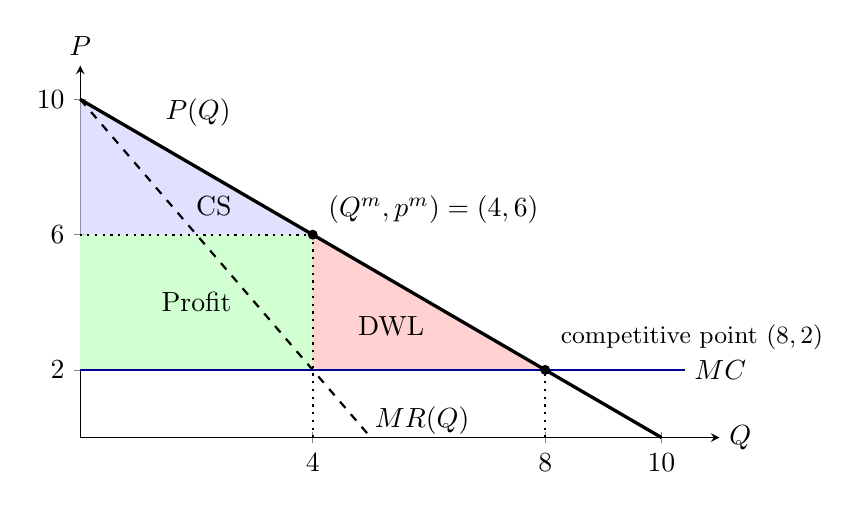
\begin{tikzpicture}
\begin{axis}[
  width=0.80\textwidth, height=0.52\textwidth,
  axis lines=left,
  xmin=0, xmax=11, ymin=0, ymax=11,
  xlabel={$Q$}, ylabel={$P$},
  xtick={4,8,10}, ytick={2,6,10},
  every axis x label/.style={at={(current axis.right of origin)}, anchor=west},
  every axis y label/.style={at={(current axis.above origin)}, anchor=south},
  clip=false]
  \fill[blue!12] (axis cs:0,6) -- (axis cs:0,10) -- (axis cs:4,6) -- cycle;
  \fill[green!18] (axis cs:0,2) rectangle (axis cs:4,6);
  \fill[red!18] (axis cs:4,6) -- (axis cs:4,2) -- (axis cs:8,2) -- cycle;
  \addplot[very thick, black, domain=0:10] {10 - x};
  \addplot[thick, dashed, black, domain=0:5] {10 - 2*x};
  \addplot[thick, blue!60!black, domain=0:10.4] {2};
  \draw[dotted, thick] (axis cs:4,0) -- (axis cs:4,6) -- (axis cs:0,6);
  \draw[dotted, thick] (axis cs:8,0) -- (axis cs:8,2);
  \fill (axis cs:4,6) circle (1.8pt);
  \fill (axis cs:8,2) circle (1.8pt);
  \node[anchor=south west] at (axis cs:4.1,6.05) {$(Q^m, p^m) = (4, 6)$};
  \node[anchor=south west, font=\small] at (axis cs:8.1,2.3) {competitive point $(8, 2)$};
  \node[anchor=south west] at (axis cs:1.3,8.9) {$P(Q)$};
  \node[anchor=west] at (axis cs:4.9,0.5) {$MR(Q)$};
  \node[anchor=west] at (axis cs:10.4,2) {$MC$};
  \node at (axis cs:2.3,6.85) {CS};
  \node at (axis cs:2,4) {Profit};
  \node at (axis cs:5.35,3.3) {DWL};
\end{axis}
\end{tikzpicture}
\caption{Monopoly with linear demand $P(Q) = 10 - Q$, marginal revenue $MR(Q) = 10 - 2Q$ and constant marginal cost
$MC = 2$. The monopolist sells $Q^m = 4$ at $p^m = 6$, while price taking would give the point $(8, 2)$. The
shaded areas are consumer surplus (CS), profit, and the deadweight loss (DWL) of pricing above marginal cost.
\Cref{sec:02-surplus} defines these areas formally. The Lerner index is $L = \frac{6 - 2}{6} = \frac{2}{3}$, which equals $\frac{1}{\varepsilon(p^m)} = \frac{2}{3}$ because
$\varepsilon(p^m) = \frac{6}{4} = \frac{3}{2}$.}
\label{fig:02-monopoly}
\end{figure}

\begin{example}[Constant-elasticity demand]\label{ex:02-ce}
Let $Q(p) = Ap^{-\varepsilon}$ with $A > 0$ and a constant $\varepsilon > 0$, and let marginal cost be strictly
positive, $c > 0$. The elasticity is the same at every price:
\[
  -Q'(p)\,\frac{p}{Q(p)} = \varepsilon A p^{-\varepsilon - 1}\cdot\frac{p}{Ap^{-\varepsilon}} = \varepsilon .
\]
If $\varepsilon > 1$, \eqref{eq:02-ce-price} is an explicit pricing formula, $p^m = \frac{\varepsilon}{\varepsilon -
1}c$. The Lerner index is the constant $\frac{1}{\varepsilon}$, and price is proportional to cost. The dollar markup
$m(p) = \frac{p}{\varepsilon}$ rises with price, so a one-dollar increase in cost raises price by
$\frac{\varepsilon}{\varepsilon - 1} > 1$ dollars. This demand curve is log-convex, so we check optimality
directly. Here $\frac{QQ''}{(Q')^2} = \frac{\varepsilon + 1}{\varepsilon}$, which is below 2 exactly when
$\varepsilon > 1$. The function $h(p) = p - c - \frac{p}{\varepsilon} = p\left(1 - \frac{1}{\varepsilon}\right) -
c$ is then strictly increasing, so the argument of \cref{lem:02-soc}(iii) shows that $p^m$ is the unique optimum. If
$\varepsilon \le 1$, revenue $Ap^{1 - \varepsilon}$ does not fall as price rises while cost $cAp^{-\varepsilon}$
falls, so profit rises at every price and no optimal price exists. \citet[Exercise~1.4]{Tirole1988} extends the
result to any convex cost function. With constant-elasticity demand and $\varepsilon > 1$, profit is then
quasi-concave in price. The boundary case $c = 0$, which \cref{ass:02-monopoly} allows, behaves differently
because profit equals revenue $Ap^{1 - \varepsilon}$. For $\varepsilon > 1$ profit rises without bound as price
falls toward zero, and the formula's value $p^m = 0$ is not an admissible price, so no optimum exists. For
$\varepsilon = 1$ profit equals $A$ at every price, so every positive price is optimal. For $\varepsilon < 1$
profit rises without bound in price.
\end{example}

\begin{example}[Exponential demand]\label{ex:02-exponential}
Let $Q(p) = e^{\frac{a - p}{b}}$ with $b > 0$, or equivalently $P(Q) = a - b\ln Q$. Then $Q'(p) = -\frac{1}{b}Q(p)$,
so the semi-elasticity is the constant $\frac{1}{b}$ and the dollar markup is $m(p) = -\frac{Q(p)}{Q'(p)} = b$ at
every price. The monopoly price is
\[
  p^m = c + b .
\]
A monopolist facing this demand charges a fixed dollar margin whatever its cost, so each dollar of cost passes
fully into price, exactly as under perfect competition. The elasticity $\varepsilon(p) = \frac{p}{b}$ rises with
price. Since $\ln Q = \frac{a - p}{b}$ is linear, and hence weakly concave, \cref{lem:02-soc} applies.
\end{example}

\begin{example}[The Bulow-Pfleiderer family]\label{ex:02-bp}
Consider demand curves of the form
\begin{equation}\label{eq:02-bp-demand}
  Q(p) = B\,\lvert\bar p - p\rvert^{g}, \qquad B > 0,
\end{equation}
on the range $p < \bar p$ when $g > 0$, and on the range $p > \bar p$ when $g < 0$. When $g > 0$, the parameter
$\bar p$ is the choke price, the highest willingness to pay. \citet{BulowPfleiderer1983} identified this family as
the one with constant pass-through of cost to price (\cref{sec:02-passthrough}). \citet{GenesoveMullin1998} write
it as $Q = \beta(\alpha - P)^{\gamma}$ and use it for the demand for refined sugar (\cref{ch:conduct}). They motivate
it by noting that linear and log-linear demand, the usual choices in industry studies, impose strong restrictions on
the monopoly pricing rule.

In both cases $\frac{\dd \ln Q}{\dd p} = -\frac{g}{\bar p - p}$. Hence the dollar markup and the elasticity are
\[
  m(p) = \frac{\bar p - p}{g}, \qquad \varepsilon(p) = \frac{p}{m(p)} = \frac{gp}{\bar p - p},
\]
both positive on the relevant range. The first-order condition $p - c = m(p)$ is linear in $p$:
\begin{align*}
  g(p - c) &= \bar p - p, \\
  (1 + g)p &= \bar p + gc, \\
  p^m &= \frac{\bar p + gc}{1 + g} .
\end{align*}
The monopoly price is affine in cost, with slope $\frac{g}{1 + g}$. Substituting $p^m$ into $\varepsilon(p)$ gives
the elasticity at the optimum, $\varepsilon(p^m) = \frac{\bar p + gc}{\bar p - c}$. The family nests the cases above.
\begin{itemize}
  \item With $g = 1$, $\bar p = a$ and $B = \frac{1}{b}$, demand is linear and $p^m = \frac{a + c}{2}$.
  \item With $g = 2$, demand is quadratic and convex, and $p^m = \frac{\bar p + 2c}{3}$.
  \item With $\bar p = 0$ and $g < 0$, demand is $Q = Bp^{g}$, which has constant elasticity $\varepsilon = -g$.
  Then $p^m = \frac{gc}{1 + g} = \frac{\varepsilon}{\varepsilon - 1}c$, which requires $g < -1$ and $c > 0$.
  \item Let $\bar p \to \infty$ and $g \to \infty$ with $\lambda_s = \frac{g}{\bar p}$ held fixed, and set
  $B = A\bar p^{-g}$ for a constant $A > 0$. Then
  \[
    Q(p) = A\left(1 - \frac{p}{\bar p}\right)^{g} = A\left(1 - \frac{\lambda_s p}{g}\right)^{g} \to A e^{-\lambda_s p} .
  \]
  The limit is exponential demand with semi-elasticity $\lambda_s$. The monopoly price converges to
  \[
    p^m = \frac{\frac{\bar p}{g} + c}{\frac{1}{g} + 1} \to c + \frac{1}{\lambda_s},
  \]
  which matches \cref{ex:02-exponential} with $b = \frac{1}{\lambda_s}$.
\end{itemize}
In inverse form, the case $g > 0$ reads $P(Q) = a - bQ^{\gamma}$ with $a = \bar p$, $b = B^{-\gamma}$ and
$\gamma = \frac{1}{g}$. The case $g < 0$ inverts to $P(Q) = \bar p + B^{-\gamma}Q^{\gamma}$, which is the same form
with $b = -B^{-\gamma}$. The symbol $\gamma$ is local to this family. The second-order condition holds
automatically when $g > 0$, because $\ln Q$ is then concave. When $g < 0$, $\frac{QQ''}{(Q')^2} = 1 - \frac{1}{g}$,
which is below 2 exactly when $g < -1$, the condition found above. The family returns in
\cref{sec:02-conduct,sec:02-passthrough} and in \cref{ch:conduct}.
\end{example}

\section{Games and equilibrium}\label{sec:02-games}

A monopolist solves a decision problem. With two or more firms, each firm's best choice depends on what its rivals
do, and we need a rule that predicts the outcome of this interdependence. This section collects the tools from
noncooperative game theory that the rest of the chapter uses. They are Nash equilibrium in pure and mixed
strategies, reaction functions, and subgame perfection in games that unfold in stages. We follow
\citet[ch.~11 and the introduction to Part~II]{Tirole1988}, which presents these tools for industrial organization.
\citet{FudenbergTirole1991} give a complete treatment.

\subsection{Nash equilibrium}\label{sec:02-nash}

\begin{definition}[Normal-form game]\label{def:02-game}
A \emph{normal-form game} has players $i = 1, \dots, N$. Player $i$ chooses an \emph{action} $a_i$ from a set $A_i$
and receives the payoff $\pi_i(a)$, where $a = (a_1, \dots, a_N)$ is the \emph{action profile}. We write $a_{-i}$
for the actions of the players other than $i$, and $(a_i', a_{-i})$ for the profile in which player $i$ switches to
$a_i'$ while the others keep $a_{-i}$.
\end{definition}

In the games of this chapter the players are firms, the actions are outputs or prices, and the payoffs are profits.
All players choose at the same time, and the structure of the game is common knowledge. A \emph{pure strategy}
picks one action with certainty. A \emph{mixed strategy} $\sigma_i$ is a probability distribution over $A_i$.
Players randomize independently, and payoffs under mixed strategies are expected values of pure-strategy payoffs. A
pure strategy is the special case of a distribution that puts probability one on a single action.

\begin{definition}[Best response and Nash equilibrium]\label{def:02-nash}
Player $i$'s \emph{best response} to $a_{-i}$ is the set $BR_i(a_{-i}) = \argmax_{a_i \in A_i}\pi_i(a_i, a_{-i})$.
A \emph{pure-strategy Nash equilibrium} is a profile $a^*$ such that
\begin{equation}\label{eq:02-nash}
  \pi_i(a_i^*, a_{-i}^*) \ge \pi_i(a_i, a_{-i}^*) \qquad \text{for every player } i \text{ and every } a_i \in A_i ,
\end{equation}
that is, $a_i^* \in BR_i(a_{-i}^*)$ for every $i$. A \emph{mixed-strategy Nash equilibrium} is a profile of
distributions $(\sigma_1^*, \dots, \sigma_N^*)$ that satisfies \eqref{eq:02-nash} with distributions in place of
actions and expected payoffs in place of payoffs.
\end{definition}

In a Nash equilibrium each player's choice is optimal given the choices of the others, and each player anticipates
those choices correctly. No player can gain by changing its own action alone. Mixed equilibria have one further
property that we use repeatedly. A player who randomizes must be indifferent among all actions in the support of its
distribution. If one of them paid strictly more, moving probability toward it would raise the expected payoff. The
indifference conditions therefore pin down the rivals' distributions. In \emph{matching pennies}, two players each
choose heads or tails. Player 1 wins one dollar from player 2 when the choices match and loses one dollar otherwise.
No pure equilibrium exists. In the mixed equilibrium each player chooses heads with probability $\frac{1}{2}$, the
only probability that leaves the opponent indifferent \citep[sec.~11.2]{Tirole1988}.

\begin{theorem}[Existence of Nash equilibrium]\label{thm:02-existence}
Suppose that each action set $A_i$ is a nonempty, compact and convex subset of a Euclidean space. Suppose also that
each payoff $\pi_i(a)$ is continuous in $a$ and quasi-concave in $a_i$. Then a pure-strategy Nash equilibrium
exists. In particular, a game with finitely many players and finitely many actions has a mixed-strategy Nash
equilibrium.
\end{theorem}

\begin{proof}[Proof sketch]
The first statement is the special case of \citet{Debreu1952} given in \citet[sec.~11.6.1]{Tirole1988}. The
standard argument applies Kakutani's fixed-point theorem (\cref{thm:B-kakutani}) to the joint best-response
correspondence
$a \mapsto BR_1(a_{-1}) \times \dots \times BR_N(a_{-N})$. Berge's maximum theorem concerns a continuous function of
a choice variable and a parameter, maximized over a fixed compact set. It says that the maximizers, as a
correspondence of the parameter, have nonempty compact values and a closed graph. Applied to each player, with
rivals' actions as the parameter, it makes the joint correspondence nonempty valued with a closed graph.
Quasi-concavity makes its values convex.
A fixed point of the correspondence is a Nash equilibrium (see also \cref{cor:B-nash-existence}). For the second
statement, a mixed strategy of player $i$
is a point in the simplex of distributions over its finite action set, which is compact and convex. The expected
payoff is linear, hence quasi-concave, in the player's own mixture. It is a polynomial, hence continuous, in the
profile of mixtures. The first statement therefore applies to the game in mixed strategies \citep{Nash1950}.
\end{proof}

Both assumptions of the theorem can fail in oligopoly models. Without quasi-concavity, best responses can jump, and a
pure equilibrium may fail to exist (\cref{rem:02-cournot-routes}). Continuity fails in the price games of
\cref{sec:02-bertrand}, because a firm's sales jump when its price crosses a rival's price. With capacity
constraints, pure equilibria may then fail to exist (\cref{sec:02-capacity}). For games with discontinuous payoffs,
\citet{DasguptaMaskin1986} give conditions for a pure equilibrium when payoffs are quasi-concave and for a mixed
equilibrium when they are not \citep[sec.~11.6.1]{Tirole1988}.

\subsection{Reaction functions}\label{sec:02-reaction}

Most models in this chapter have one-dimensional actions and smooth payoffs. Take two firms with actions
$a_1, a_2 \in \R$ and twice continuously differentiable profits, and suppose each profit is strictly concave in the
firm's own action. The first-order condition $\frac{\partial \pi_i}{\partial a_i}(a_i, a_j) = 0$ then defines firm
$i$'s \emph{reaction function} $R_i(a_j)$, its unique best response to $a_j$ at an interior optimum. A Nash
equilibrium is a pair with $a_1^* = R_1(a_2^*)$ and $a_2^* = R_2(a_1^*)$, an intersection of the two reaction curves.
Suppose in addition that the strict second-order condition $\frac{\partial^2 \pi_i}{\partial a_i^2}(R_i(a_j), a_j) <
0$ holds. Strict concavity alone does not deliver it. The payoff $\pi_i = -a_i^4 + a_i a_j$ is strictly concave in
$a_i$, yet its second derivative vanishes at the best response $a_i = 0$ to $a_j = 0$. There its reaction function
$R_i(a_j) = \left(\frac{a_j}{4}\right)^{\frac{1}{3}}$ has an infinite slope. Under the strict condition, the implicit
function theorem makes $R_i$ continuously differentiable. Differentiating the identity
$\frac{\partial \pi_i}{\partial a_i}(R_i(a_j), a_j) = 0$ with respect to $a_j$ gives
\[
  \frac{\partial^2 \pi_i}{\partial a_i^2}\,R_i'(a_j) + \frac{\partial^2 \pi_i}{\partial a_i\,\partial a_j} = 0 ,
\]
so the slope of the reaction function is
\begin{equation}\label{eq:02-reaction-slope}
  R_i'(a_j) = -\frac{\frac{\partial^2 \pi_i}{\partial a_i\,\partial a_j}}{\frac{\partial^2 \pi_i}{\partial a_i^2}}
\end{equation}
\citep[introduction to Part~II, eq.~(5)]{Tirole1988}. The denominator is negative by the strict second-order
condition, so the slope of the reaction
function has the sign of the cross-partial derivative. Following \citet{BulowGeanakoplosKlemperer1985}, actions are \emph{strategic
substitutes} when the cross-partial is negative and \emph{strategic complements} when it is positive. Quantities are
often substitutes and prices often complements (\cref{sec:02-cournot-br} and \cref{rem:02-strategic}).

Reaction functions are a device for finding equilibria. They do not describe behavior in a simultaneous-move game,
since no firm observes its rival's choice before it acts. The reaction function states what a firm would do if it
learned that its rival had changed its action \citep[introduction to Part~II]{Tirole1988}. The point returns in the
critique of conjectural variations (\cref{sec:02-interpret}).

\subsection{Subgame perfection}\label{sec:02-spe}

Several models in this chapter unfold over time. Firms enter and then compete (\cref{sec:02-entry}), build capacity
and then set prices (\cref{sec:02-capacity}), or play the same game repeatedly (\cref{sec:02-repeated}). An
\emph{extensive-form game} describes such a situation. It specifies the order of moves, the actions available at each
move, what each player knows when it moves, and the payoffs at the end of each path of play. The points at which a
player moves but cannot tell apart form one of its \emph{information sets}. A strategy is a complete plan of action.
It specifies a move at every point where the player could be called upon to act, including points that are never
reached when the plan is followed.

Nash equilibrium is too permissive in these games, because it can rest on threats that a player would not carry out.
Consider an entrant that either stays out or enters. Staying out gives the entrant 0 and the incumbent 2. After entry,
the incumbent either accommodates, which gives both firms 1, or fights, which gives the entrant $-1$ and the
incumbent 0. The profile in which the entrant stays out and the incumbent plans to fight is a Nash equilibrium. Given
the plan to fight, entry would earn $-1$. Given that entry does not occur, the plan costs the incumbent nothing. Yet
the threat is not credible, because after entry the incumbent earns 1 by accommodating and 0 by fighting.

\begin{definition}[Subgame-perfect equilibrium]\label{def:02-spe}
A \emph{subgame} is a part of an extensive-form game that begins at a point where the mover knows the entire history
of play, and that contains every later move. It does not split an information set, so two points that a player
cannot tell apart are both inside the subgame or both outside it. A \emph{subgame-perfect equilibrium} is a strategy
profile that induces a Nash equilibrium in every subgame \citep{Selten1965}.
\end{definition}

The whole game is one of its subgames, so a subgame-perfect equilibrium is a Nash equilibrium. Perfection adds the
requirement that strategies remain optimal off the equilibrium path. In games of \emph{perfect information}, where
every mover knows all earlier actions, subgame-perfect equilibria are found by \emph{backward induction}
\citep{Kuhn1953}. We solve the last mover's problem at each of its decision points and replace those points by the
resulting payoffs. We then repeat the step until we reach the first move. In the entry game the incumbent accommodates
after entry. The entrant anticipates this and enters, and this is the unique subgame-perfect equilibrium
\citep[secs.~11.3 and 11.3.1]{Tirole1988}.

Most games in this book have \emph{almost perfect information}. Play proceeds in stages, players move simultaneously
within a stage, and everyone observes all earlier stages. Backward induction then works stage by stage. The last
stage is solved as a Nash equilibrium after every history. Each earlier stage is then solved as a game whose payoffs
are the equilibrium payoffs of the stages that follow. The two-stage entry game of \cref{def:02-entry-game} and the
capacity game of \cref{prop:02-ks} are solved in this way. The second-stage equilibrium gives a reduced-form payoff
for each first-stage choice, and the first stage is a game in those payoffs. Repeated games are the other leading
case, and \cref{sec:02-repeated} states the two results on them that the chapter uses.

\section{Cournot oligopoly with \texorpdfstring{$N$}{N} firms}\label{sec:02-cournot}

The Cournot model is the workhorse model of oligopoly with a homogeneous good. It delivers the link between
concentration and margins that motivated a generation of empirical work (\cref{ch:intro}). Its comparative statics
underlie the analysis of entry, mergers and cost pass-through in later sections and chapters. This section develops
the model for $N$ firms with general demand and asymmetric convex costs. We prove existence and uniqueness, derive
the relation between margins and concentration, solve the linear case in closed form and sign the comparative
statics.

\subsection{The game}\label{sec:02-cournot-game}

\begin{definition}[Cournot game]\label{def:02-cournot}
$N$ firms produce a homogeneous good. Firm $i$ chooses an output $q_i \ge 0$. All firms choose simultaneously and
have complete information. Given the output vector $q = (q_1, \dots, q_N)$, industry output is $Q = \sum_i q_i$,
the market price is $P(Q)$, and firm $i$'s profit is
\[
  \pi_i(q) = P(Q)\,q_i - C_i(q_i) .
\]
A \emph{Cournot equilibrium} is a Nash equilibrium in quantities (\cref{def:02-nash}), an output vector $q^*$ such that
$\pi_i(q_i^*, q_{-i}^*) \ge \pi_i(q_i, q_{-i}^*)$ for every firm $i$ and every $q_i \ge 0$.
\end{definition}

Here $q_{-i}$ is the vector of rivals' outputs and $Q_{-i} = Q - q_i$ is their total. Firm $i$'s profit depends on
its rivals only through $Q_{-i}$, so we also write it as $\pi_i(q_i, Q_{-i})$.

\begin{assumption}[Cournot regularity]\label{ass:02-cournot}
\leavevmode
\begin{enumerate}[label=(C\arabic*)]
  \item Inverse demand $P$ is twice continuously differentiable on $[0, \infty)$, with $P'(Q) < 0$ for every $Q$.
  \item For every $Q > 0$, $P'(Q) + QP''(Q) < 0$. Equivalently, $P'(Q) + qP''(Q) < 0$ for every $q \in [0, Q]$.
  \item Each cost function $C_i$ is twice continuously differentiable, nondecreasing and convex on $[0, \infty)$,
  so that $C_i' \ge 0$ and $C_i'' \ge 0$.
  \item There is $\bar Q > 0$ with $P(\bar Q) \le \min_i C_i'(0)$, and $P(0) > C_i'(0)$ for at least one firm $i$.
\end{enumerate}
\end{assumption}

Condition (C1) says that demand slopes down. In (C2), the two forms are equivalent because $P' + qP''$ is linear in
$q$ and negative at $q = 0$, so it is negative on $[0, Q]$ if and only if it is negative at $q = Q$. We show below
that (C2) makes each firm's marginal revenue fall when its rivals produce more. Condition (C3) allows constant or
rising marginal cost. Condition (C4) says that no firm wants to produce once industry output reaches $\bar Q$,
while at least one firm would produce if no one else did.

\begin{remark}[Interpreting (C2)]\label{rem:02-c2}
Define the \emph{curvature} of inverse demand as $\chi(Q) = -\frac{QP''(Q)}{P'(Q)}$. Since $P' < 0$, (C2) is the
condition $\chi(Q) < 1$ at every $Q$. Linear demand has $\chi = 0$, and every concave inverse demand has
$\chi \le 0$, so both satisfy (C2). The family $P = a - bQ^{\gamma}$ of \cref{ex:02-bp} with $b, \gamma > 0$ has
$\chi = 1 - \gamma < 1$ and also satisfies it. Constant-elasticity demand $P(Q) = \left(\frac{Q}{A}\right)^{-\frac{1}{\varepsilon}}$
has $\chi = 1 + \frac{1}{\varepsilon} > 1$ and violates it. For this demand, the inequality
$P'(Q) + q_iP''(Q) < 0$ holds if and only if $s_i\left(1 + \frac{1}{\varepsilon}\right) < 1$. The arguments below
therefore apply at equilibria in which no firm's share exceeds $\frac{\varepsilon}{1 + \varepsilon}$.
\citet{Novshek1985} shows that a condition of the type in (C2), namely that each firm's marginal revenue falls when
its rivals' output rises, guarantees existence of an equilibrium even without convex costs. Curvature also governs
pass-through (\cref{sec:02-passthrough}).
\end{remark}

\subsection{Best responses and strategic substitutes}\label{sec:02-cournot-br}

Firm $i$ takes $Q_{-i}$ as given and chooses $q_i$. Its \emph{best response} $BR_i(Q_{-i})$ is the output that
maximizes $\pi_i(q_i, Q_{-i})$.

\begin{lemma}[Concavity and best responses]\label{lem:02-cournot-br}
Under \cref{ass:02-cournot}, $\pi_i(q_i, Q_{-i})$ is strictly concave in $q_i$ for every $Q_{-i} \ge 0$. The best
response is unique and is characterized by the conditions
\begin{equation}\label{eq:02-cournot-foc}
  P(Q) + q_iP'(Q) - C_i'(q_i) \le 0, \qquad q_i \ge 0, \qquad q_i\left[P(Q) + q_iP'(Q) - C_i'(q_i)\right] = 0,
\end{equation}
with $Q = q_i + Q_{-i}$. Where $BR_i(Q_{-i}) > 0$, the best response is differentiable with slope
\begin{equation}\label{eq:02-br-slope}
  BR_i'(Q_{-i}) = -\frac{P'(Q) + q_iP''(Q)}{2P'(Q) + q_iP''(Q) - C_i''(q_i)} \in (-1, 0) .
\end{equation}
\end{lemma}

\begin{proof}
The derivative of profit with respect to own output is
\[
  \frac{\partial \pi_i}{\partial q_i} = P(Q) + q_iP'(Q) - C_i'(q_i) .
\]
Differentiating again and grouping terms,
\[
  \frac{\partial^2 \pi_i}{\partial q_i^2} = 2P'(Q) + q_iP''(Q) - C_i''(q_i)
    = \left[P'(Q) + q_iP''(Q)\right] + \left[P'(Q) - C_i''(q_i)\right] .
\]
The first bracket is negative by (C2), because $q_i \le Q$. The second is negative by (C1) and (C3). So profit is
strictly concave in $q_i$. For $q_i \ge \bar Q$ we have $Q \ge \bar Q$, and then
$\frac{\partial \pi_i}{\partial q_i} < P(\bar Q) - C_i'(0) \le 0$ by (C4). A maximizer therefore exists on
$[0, \bar Q]$. Strict concavity makes it unique and makes the Kuhn-Tucker conditions \eqref{eq:02-cournot-foc}
necessary and sufficient.

Where $BR_i > 0$, the first-order condition holds with equality. Write it as $G(q_i, Q_{-i}) = 0$ with
$G(q_i, Q_{-i}) = P(q_i + Q_{-i}) + q_iP'(q_i + Q_{-i}) - C_i'(q_i)$. Its partial derivatives are
\[
  \frac{\partial G}{\partial q_i} = 2P' + q_iP'' - C_i'' < 0, \qquad \frac{\partial G}{\partial Q_{-i}} = P' + q_iP'' .
\]
By the implicit function theorem (\cref{app:math}), $BR_i'(Q_{-i}) = -\left(\frac{\partial G}{\partial
q_i}\right)^{-1}\frac{\partial G}{\partial Q_{-i}}$, which is \eqref{eq:02-br-slope}. Both the numerator and the denominator are negative. The
denominator equals the numerator plus the negative term $P' - C_i''$, so the ratio
$\frac{P' + q_iP''}{2P' + q_iP'' - C_i''}$ lies in $(0, 1)$. Hence $BR_i' \in (-1, 0)$.
\end{proof}

The cross-partial derivative of profit is $\frac{\partial^2 \pi_i}{\partial q_i \partial Q_{-i}} = P'(Q) +
q_iP''(Q) < 0$. More output by rivals therefore lowers firm $i$'s marginal profit. The slope \eqref{eq:02-br-slope}
is the general formula \eqref{eq:02-reaction-slope}, with this cross-partial in the numerator and the own second
derivative $2P' + q_iP'' - C_i''$ in the denominator. In the terminology of
\citet{BulowGeanakoplosKlemperer1985}, quantities are \emph{strategic substitutes}: a more aggressive strategy by
one firm lowers its rivals' marginal profits (p.~489). Best responses slope down as a result. The bound
$BR_i' > -1$ adds that a firm offsets only part of a rival's expansion. When rivals produce one more unit, firm $i$
contracts by less than one unit, and industry output rises. This property drives every comparative static below.
With linear demand $P = a - bQ$ and constant cost $c_i$, the best response is $BR_i(Q_{-i}) = \max\left\{0,
\frac{a - c_i - bQ_{-i}}{2b}\right\}$, with slope $-\frac{1}{2}$ where positive.

\subsection{Existence and uniqueness}\label{sec:02-cournot-exist}

An equilibrium solves $N$ best-response conditions simultaneously. Because each firm's profit depends on its rivals
only through their total output, the system reduces to a single equation in industry output.
\citet{SzidarovszkyYakowitz1977} and \citet{Novshek1985} use this reduction, and \citet{Vives1999} develops it for
general aggregative games. The device is the following function.

\begin{definition}[Replacement function]\label{def:02-replacement}
For $Q \in [0, \bar Q]$, the \emph{replacement function} $\tilde q_i(Q)$ of firm $i$ is the output that satisfies
the conditions \eqref{eq:02-cournot-foc} when industry output equals $Q$:
\[
  \tilde q_i(Q) = 0 \ \text{ if } P(Q) \le C_i'(0), \qquad
  P(Q) + \tilde q_i(Q)P'(Q) = C_i'(\tilde q_i(Q)) \ \text{ otherwise}.
\]
\end{definition}

The replacement function gives the output that firm $i$ would choose if it knew that industry output, including its
own, would equal $Q$. It is well defined. Let $G_i(q, Q) = P(Q) + qP'(Q) - C_i'(q)$. For fixed $Q$, $G_i$ is
strictly decreasing in $q$, because $\frac{\partial G_i}{\partial q} = P'(Q) - C_i''(q) < 0$. It also tends to
$-\infty$ as $q \to \infty$, because $G_i(q, Q) \le P(Q) + qP'(Q)$. So when $G_i(0, Q) = P(Q) - C_i'(0) > 0$ there
is exactly one positive root. By construction, $q_i$ is a best response to $Q_{-i}$ if and only if
$q_i = \tilde q_i(q_i + Q_{-i})$.

\begin{lemma}[Properties of replacement functions]\label{lem:02-replacement}
Under \cref{ass:02-cournot}, the following hold for each firm $i$.
\begin{enumerate}[label=(\roman*)]
  \item $\tilde q_i$ is continuous on $[0, \bar Q]$ and $\tilde q_i(\bar Q) = 0$. If $\tilde q_i(Q) = 0$, then
  $\tilde q_i(Q') = 0$ for every $Q' \ge Q$.
  \item At any $Q$ with $0 < \tilde q_i(Q) \le Q$, $\tilde q_i$ is differentiable and
  \begin{equation}\label{eq:02-replacement-slope}
    \tilde q_i'(Q) = -\frac{P'(Q) + \tilde q_i(Q)P''(Q)}{P'(Q) - C_i''(\tilde q_i(Q))} < 0 .
  \end{equation}
  \item The set $R_i = \{Q \in [0, \bar Q] : \tilde q_i(Q) \le Q\}$ is a closed interval that contains $\bar Q$,
  and $\tilde q_i$ is nonincreasing on $R_i$.
\end{enumerate}
\end{lemma}

\begin{proof}
(i) Where $P(Q) > C_i'(0)$, the root of $G_i(\cdot, Q)$ is continuous in $Q$ by the implicit function theorem,
since $\frac{\partial G_i}{\partial q} < 0$. Because $C_i'(q) \ge C_i'(0)$, at the root we have
$0 = G_i \le P(Q) - C_i'(0) + \tilde q_i(Q)P'(Q)$, which gives the bound
\[
  \tilde q_i(Q) \le \frac{P(Q) - C_i'(0)}{-P'(Q)} .
\]
The bound tends to zero as $P(Q)$ falls to $C_i'(0)$, so $\tilde q_i$ is continuous at the point where it reaches
zero. By (C4), $P(\bar Q) \le C_i'(0)$, so $\tilde q_i(\bar Q) = 0$. Since $P$ is decreasing, $P(Q) \le C_i'(0)$
implies $P(Q') \le C_i'(0)$ for every $Q' \ge Q$.

(ii) At such a $Q$, $G_i(\tilde q_i(Q), Q) = 0$ with $\frac{\partial G_i}{\partial q} = P' - C_i'' < 0$ and
$\frac{\partial G_i}{\partial Q} = P'(Q) + \tilde q_i(Q)P''(Q)$. The latter is negative by (C2), because
$\tilde q_i(Q) \le Q$. The implicit function theorem gives \eqref{eq:02-replacement-slope}, a ratio of two negative
numbers with a minus sign in front.

(iii) The set $R_i$ is closed because $\tilde q_i$ is continuous, and it contains $\bar Q$ because
$\tilde q_i(\bar Q) = 0$. Take $Q' \in R_i$ and suppose that some $Q'' > Q'$ lies outside $R_i$. Let $Q^\circ$ be
the largest point of $[Q', Q'']$ in $R_i$. Then $Q^\circ < Q''$, and continuity forces $\tilde q_i(Q^\circ) =
Q^\circ$, with $\tilde q_i(Q) > Q$ on $(Q^\circ, Q'']$. If $Q^\circ = 0$, then $\tilde q_i(0) = 0$ and by (i)
$\tilde q_i \equiv 0$, a contradiction. So $\tilde q_i(Q^\circ) = Q^\circ > 0$, and by (ii) the function
$\tilde q_i(Q) - Q$ has derivative below $-1$ at $Q^\circ$. It is therefore negative just above $Q^\circ$, which
contradicts the choice of $Q^\circ$. Hence $R_i$ is an interval. On $R_i$, $\tilde q_i$ is strictly decreasing where
it is positive, by (ii), and it stays at zero once it reaches zero, by (i). So it is nonincreasing on $R_i$.
\end{proof}

\begin{proposition}[Existence and uniqueness of Cournot equilibrium]\label{prop:02-cournot-exist}
Under \cref{ass:02-cournot}, a Cournot equilibrium exists and is unique. Industry output $Q^*$ is the unique root
in $(0, \bar Q)$ of
\begin{equation}\label{eq:02-aggregate-eq}
  \Phi(Q) \equiv \sum_{i=1}^N \tilde q_i(Q) - Q = 0,
\end{equation}
and firm $i$ produces $q_i^* = \tilde q_i(Q^*)$. Moreover, $\Phi(Q) > 0$ for $0 \le Q < Q^*$ and $\Phi(Q) < 0$ for
$Q^* < Q \le \bar Q$.
\end{proposition}

\begin{proof}
We proceed in four steps.
\begin{enumerate}[label=\arabic*.]
  \item \emph{Equilibria are roots of $\Phi$.} By \cref{lem:02-cournot-br}, $q^*$ is an equilibrium if and only if
  every $q_i^*$ satisfies \eqref{eq:02-cournot-foc} at $Q^* = \sum_j q_j^*$. If $Q^* \le \bar Q$, this says exactly
  that $q_i^* = \tilde q_i(Q^*)$ for every $i$, and summing gives $\Phi(Q^*) = 0$. Equilibrium output cannot be
  zero, because the firm with $P(0) > C_i'(0)$ in (C4) would then gain by producing. It cannot be at least
  $\bar Q$ either. Any firm with $q_i^* > 0$ would then satisfy $C_i'(q_i^*) = P(Q^*) + q_i^*P'(Q^*) < P(\bar Q)
  \le C_i'(0)$, which contradicts (C3). So all outputs would be zero, a contradiction. Conversely, every root
  $Q^* \in (0, \bar Q)$ of $\Phi$ yields the equilibrium $q_i^* = \tilde q_i(Q^*)$.
  \item \emph{Location of roots.} At a root, $\tilde q_i(Q^*) \le \sum_j \tilde q_j(Q^*) = Q^*$ for every $i$, so
  $Q^*$ lies in $R = \bigcap_i R_i$. By \cref{lem:02-replacement}(iii), $R$ is a closed interval $[Q_0, \bar Q]$.
  \item \emph{Uniqueness.} Each $\tilde q_i$ is nonincreasing on $R$, and $-Q$ is strictly decreasing, so $\Phi$ is
  strictly decreasing on $R$ and has at most one root there.
  \item \emph{Existence and sign.} The firm $k$ of (C4) has $\tilde q_k(0) > 0$, so $0 \notin R_k$ and
  $Q_0 > 0$. Let $j$ be a firm with $\min R_j = Q_0$. Continuity gives $\tilde q_j(Q_0) = Q_0$, so
  $\Phi(Q_0) \ge \tilde q_j(Q_0) - Q_0 = 0$. For $Q < Q_0$, $Q \notin R_j$, so $\Phi(Q) \ge \tilde q_j(Q) - Q > 0$.
  At the other end, $\Phi(\bar Q) = -\bar Q < 0$. The intermediate value theorem yields a root in $[Q_0, \bar Q)$.
  Strict monotonicity on $R$ and positivity below $Q_0$ give the sign pattern. \qedhere
\end{enumerate}
\end{proof}

\Cref{fig:02-replacement} illustrates the construction for a linear market with three firms. With $P(Q) = 10 - Q$
and constant costs $c_i$, the condition $P(Q) + qP'(Q) = c_i$ reads $10 - Q - q = c_i$, so
$\tilde q_i(Q) = \max\{0, 10 - c_i - Q\}$. With costs $(1, 2, 3)$ the replacement functions are $9 - Q$, $8 - Q$
and $7 - Q$ where positive. For $Q \le 7$ their sum is $24 - 3Q$, and setting it equal to $Q$ gives $Q^* = 6$ and
outputs $(3, 2, 1)$. Firm 1's replacement function exceeds $Q$ for $Q < 4.5$, so $R = [4.5, 9]$, with $\bar Q = 9$
because $P(9) = 1$ equals the lowest marginal cost.

\begin{figure}[htbp]
\centering
\begin{tikzpicture}
\begin{axis}[
  width=0.80\textwidth, height=0.56\textwidth,
  axis lines=left,
  xmin=0, xmax=10.2, ymin=0, ymax=12.5,
  xlabel={Industry output $Q$}, ylabel={Output},
  xtick={0,2,4,6,8,10}, ytick={0,2,4,6,8,10,12}, yticklabels={0,2,4,6,,,12},
  every axis x label/.style={at={(current axis.right of origin)}, anchor=north east, yshift=-16pt},
  every axis y label/.style={at={(current axis.above origin)}, anchor=south, yshift=2pt},
  clip=false]
  \addplot[thick, black, domain=0:10, samples=201] {max(0, 9 - x)};
  \addplot[thick, black!60, domain=0:10, samples=201] {max(0, 8 - x)};
  \addplot[thick, black!35, domain=0:10, samples=201] {max(0, 7 - x)};
  \addplot[very thick, blue!70!black, domain=4:10, samples=401] {max(0,9-x)+max(0,8-x)+max(0,7-x)};
  \addplot[thick, dashed, red!70!black, domain=0:10] {x};
  \draw[dotted, thick] (axis cs:6,0) -- (axis cs:6,6);
  \fill (axis cs:6,6) circle (1.8pt);
  \fill (axis cs:6,3) circle (1.5pt);
  \fill (axis cs:6,2) circle (1.5pt);
  \fill (axis cs:6,1) circle (1.5pt);
  \node[anchor=east, font=\small] at (axis cs:-0.1,9) {$\tilde q_1(Q)$};
  \node[anchor=east, font=\small] at (axis cs:-0.1,8) {$\tilde q_2(Q)$};
  \node[anchor=east, font=\small] at (axis cs:-0.1,7) {$\tilde q_3(Q)$};
  \node[anchor=west, blue!70!black] at (axis cs:4.3,12.0) {$\sum_i \tilde q_i(Q)$};
  \node[anchor=west, red!70!black] at (axis cs:10.0,10.0) {$45^\circ$ line};
  \node[anchor=east] (qstar) at (axis cs:4.9,7.4) {$Q^* = 6$};
  \draw[-{Stealth[length=5pt]}, thin] (qstar.east) -- (axis cs:5.92,6.12);
  \node[anchor=west, font=\footnotesize] at (axis cs:6.12,3.5) {$q_1^*$};
  \node[anchor=west, font=\footnotesize] at (axis cs:6.12,2.2) {$q_2^*$};
  \node[anchor=west, font=\footnotesize] at (axis cs:6.12,1.2) {$q_3^*$};
\end{axis}
\end{tikzpicture}
\caption{Replacement functions for $P(Q) = 10 - Q$ and constant marginal costs $(1, 2, 3)$. Each firm's replacement
function $\tilde q_i(Q) = \max\{0, 10 - c_i - Q\}$ is the output that is optimal for firm $i$ when industry output is
$Q$. Their sum, $24 - 3Q$ for $Q \le 7$, crosses the $45^\circ$ line once, at $Q^* = 6$. The equilibrium outputs
$(3, 2, 1)$ are read off the individual replacement functions at $Q^*$.}
\label{fig:02-replacement}
\end{figure}

\begin{remark}[Why uniqueness matters]\label{rem:02-uniqueness}
Empirical work uses equilibrium conditions in two ways. Estimation evaluates first-order conditions at the observed
prices and quantities, for example to invert them for marginal cost as in \eqref{eq:02-infer-mc}. It never has to
solve for an equilibrium, so multiplicity does no harm there. Counterfactuals, such as the effect of a merger or a
tax, must solve for the new equilibrium. If several solutions exist, the analyst needs a rule for selecting one, and
conclusions can depend on that rule. \Cref{prop:02-cournot-exist} rules this out for homogeneous-good Cournot markets
that satisfy (C1) to (C4). Merger simulations in practice often compute the new equilibrium by iterating on the
first-order conditions from the premerger prices, which selects an equilibrium close to the status quo.
\Cref{ch:diffprod} gives the corresponding conditions for differentiated-products price competition.
\end{remark}

\begin{remark}[Other routes to existence and uniqueness]\label{rem:02-cournot-routes}
\Cref{thm:02-existence} gives a second proof of existence. Under \cref{ass:02-cournot}, restrict each firm to the
compact and convex set $[0, \bar Q]$. Profit $\pi_i(q)$ is continuous, and by \cref{lem:02-cournot-br} it is strictly
concave, hence quasi-concave, in $q_i$. The theorem yields an equilibrium of the restricted game, and it is also an
equilibrium of the original game. The proof of \cref{lem:02-cournot-br} shows that $\frac{\partial \pi_i}{\partial
q_i} < 0$ whenever $q_i \ge \bar Q$, so no output above $\bar Q$ does better than $\bar Q$ itself. This route needs
only quasi-concavity of profit in own output, but it is silent on uniqueness. The replacement-function proof of
\cref{prop:02-cournot-exist} gives both.

\citet[sec.~5.7.1]{Tirole1988} reviews the other approaches. \citet{SzidarovszkyYakowitz1977} assume that profit is
concave in own output, which holds when costs are convex and inverse demand is concave. Profit need not be concave
when demand is sufficiently convex. \citet{Friedman1983} and \citet{RobertsSonnenschein1977} give robust examples in
which no pure-strategy equilibrium exists even with convex costs. Without concavity, reaction functions can jump.
\citet{McManus1964} and \citet{RobertsSonnenschein1976} prove existence for symmetric firms with convex costs.
Convex costs ensure that the common reaction function jumps only upward, and only a downward jump can prevent a
symmetric equilibrium. \citet{Novshek1985} works with the condition discussed in \cref{rem:02-c2}. For uniqueness
with two firms and strictly concave profits, a sufficient condition is that $\lvert BR_i'\rvert < 1$ for both firms on
the relevant range. The reaction curves then cross at most once. \Cref{lem:02-cournot-br} shows that (C1) to (C3)
deliver this bound, since $BR_i' \in (-1, 0)$.
\end{remark}

\subsection{Markups and concentration}\label{sec:02-cournot-markups}

In this subsection each firm has a constant marginal cost $c_i$. Firm $i$'s Lerner index is $L_i = \frac{P -
c_i}{P}$, and the \emph{share-weighted industry Lerner index} is $\bar L = \sum_i s_iL_i$. The market elasticity at
industry output $Q$ is $\varepsilon = -\frac{P(Q)}{QP'(Q)}$.

\begin{proposition}[Cowling and Waterson]\label{prop:02-cowling-waterson}
In a Cournot equilibrium with constant marginal costs, every active firm satisfies
\begin{equation}\label{eq:02-cw-firm}
  L_i = \frac{P - c_i}{P} = \frac{s_i}{\varepsilon},
\end{equation}
and the share-weighted industry Lerner index satisfies
\begin{equation}\label{eq:02-cowling-waterson}
  \bar L = \sum_{i=1}^N s_iL_i = \frac{\HHI}{\varepsilon} .
\end{equation}
\end{proposition}

\begin{proof}
This is \cref{prop:01-cowling-waterson}. Each active firm satisfies the first-order condition
$P(Q) + q_iP'(Q) = c_i$, and the algebra in that proof turns it into \eqref{eq:02-cw-firm}. Inactive firms have
$s_i = 0$ and add nothing to either sum, so summing $s_iL_i$ over the active firms gives
\eqref{eq:02-cowling-waterson}.
\end{proof}

The result is due to \citet{CowlingWaterson1976}. It agrees with the monopoly rule applied to residual demand. By
\eqref{eq:02-cournot-residual}, firm $i$'s residual elasticity is $\varepsilon_i^R = \frac{\varepsilon}{s_i}$, so
\eqref{eq:02-cw-firm} reads $L_i = \frac{1}{\varepsilon_i^R}$. Each Cournot firm is a monopolist on the demand
left to it by its rivals. Since $L_i < 1$ whenever $c_i > 0$, every active firm has $s_i < \varepsilon$. Cournot
firms can therefore operate where market demand is inelastic, provided that each firm's share is below the market
elasticity. A monopolist never can (\cref{prop:02-elastic}).

\begin{corollary}[Symmetric firms]\label{cor:02-cournot-symmetric}
Suppose \cref{ass:02-cournot} holds and $c_i = c$ for all $i$. Then the unique Cournot equilibrium is symmetric and
interior, with $q_i^* = \frac{Q^*}{N}$ for every firm. The formulas of \cref{cor:01-cournot-cases} hold, in
particular $\HHI = \frac{1}{N}$ and $L = \frac{P - c}{P} = \frac{1}{N\varepsilon}$.
\end{corollary}

\begin{proof}
With identical costs, all firms have the same replacement function, so by \cref{prop:02-cournot-exist} they produce
the same output $\tilde q(Q^*)$. Hence $q_i^* = \frac{Q^*}{N}$, which is positive because $Q^* > 0$. Every firm is
active with share $\frac{1}{N}$, so \cref{cor:01-cournot-cases}(i) applies. Equivalently, substitute
$s_i = \frac{1}{N}$ and $\HHI = \frac{1}{N}$ into \eqref{eq:02-cowling-waterson}.
\end{proof}

The symmetric formula shows how the number of firms disciplines margins. \Cref{prop:02-cournot-converge} below shows
that price approaches marginal cost as $N$ grows. Read literally, \eqref{eq:02-cowling-waterson} suggests that
margins should rise with concentration across industries, with slope $\frac{1}{\varepsilon}$. The next two results
show why that reading needs care.

\begin{corollary}[Efficient firms are large]\label{cor:02-efficient}
In a Cournot equilibrium with constant marginal costs, every active firm has share
\begin{equation}\label{eq:02-share-cost}
  s_i = \varepsilon\,\frac{P - c_i}{P} = \varepsilon\left(1 - \frac{c_i}{P}\right),
\end{equation}
so lower-cost firms have larger shares. If all $N$ firms are active, let $\sigma_c^2 = \frac{1}{N}\sum_i (c_i -
\tilde c)^2$ be the variance of costs around their simple average $\tilde c = \frac{1}{N}\sum_i c_i$. Then
\begin{equation}\label{eq:02-hhi-cost}
  \HHI = \frac{1}{N} + N\,\frac{\varepsilon^2}{P^2}\sigma_c^2, \qquad
  \bar L = \frac{1}{N\varepsilon} + N\,\frac{\varepsilon}{P^2}\sigma_c^2 .
\end{equation}
\end{corollary}

\begin{proof}
Equation \eqref{eq:02-share-cost} rearranges \eqref{eq:02-cw-firm}. It makes each share an affine function of the
firm's cost with slope $-\frac{\varepsilon}{P}$, so $\sigma_s^2 = \frac{\varepsilon^2}{P^2}\sigma_c^2$.
Substituting into \eqref{eq:01-hhi-variance} gives the expression for $\HHI$, and dividing it by $\varepsilon$ gives
$\bar L$ by \eqref{eq:02-cowling-waterson}.
\end{proof}

With linear demand $P = a - bQ$, the elasticity is $\varepsilon = \frac{P}{bQ}$, so $\frac{\varepsilon}{P} =
\frac{1}{bQ}$ and \eqref{eq:02-hhi-cost} reduces to \cref{prop:01-demsetz}(ii).

\Cref{cor:02-efficient} is an identity that holds at the equilibrium, since $\varepsilon$ and $P$ are themselves
equilibrium outcomes. It shows that dispersion in costs raises concentration and the average margin together, with
no change in the way firms compete. Large firms earn high margins because they are efficient. This is the formal
content of the efficiency critique of \citet{Demsetz1973}, which \cref{ch:intro} develops in the context of
cross-industry regressions.

The identity also has an industry-profit form \citep[eq.~(5.14) and Exercise~5.6]{Tirole1988}. With constant
marginal costs, industry variable profit is
\[
  \Pi = \sum_i (P - c_i)\,q_i = \sum_i \frac{s_iP}{\varepsilon}\,q_i = \frac{PQ}{\varepsilon}\sum_i s_i^2 ,
\]
where the second step uses \eqref{eq:02-cw-firm} and the third uses $q_i = s_iQ$. Dividing by revenue $PQ$ gives
\begin{equation}\label{eq:02-cw-profit}
  \frac{\Pi}{PQ} = \frac{\HHI}{\varepsilon} .
\end{equation}
Suppose consumers spend a fixed amount $E$ on the good, so that demand is $Q = \frac{E}{p}$. The elasticity is then
one and revenue equals $E$ at every price, so $\Pi = E\,\HHI$. In this case the Herfindahl index measures industry
profit exactly, up to a constant (Tirole's eq.~(5.15)).

Bertrand competition gives a sharp contrast \citep[sec.~5.5]{Tirole1988}. With symmetric firms and a common
constant marginal cost, the Bertrand price and industry profit do not depend on the number of firms
(\cref{prop:02-bertrand}), so profitability and concentration are unrelated. In Cournot competition, profitability
falls with the number of firms. With asymmetric costs $c_1 < c_2 \le c_j$ for $j \ge 3$, the lowest-cost Bertrand
firm takes the whole market at the price $\min\{c_2, p^m(c_1)\}$, where $p^m(c_1)$ is its monopoly price
(\cref{sec:02-bertrand-homog}). When $p^m(c_1) > c_2$, this outcome is an equilibrium if ties go to the low-cost
firm or if prices lie on a fine grid that contains $c_2$. With continuous prices and an equal split of ties, no pure
equilibrium exists in that case. In this outcome concentration takes its highest value under any index that satisfies the
Encaoua-Jacquemin properties, and the efficient firm earns a positive profit. Under both models, intrinsic cost
asymmetries raise concentration and profitability together, which is the argument of \citet{Demsetz1973}.

\begin{example}[Cost asymmetry raises concentration and profit]\label{ex:02-asym}
Let $Q = 1 - p$, and let two Cournot firms have costs $c_1 = c - d$ and $c_2 = c + d$, with $d \ge 0$ and
$1 - c - 3d > 0$ \citep[Exercise~5.7]{Tirole1988}. \Cref{ex:02-linear-cournot} with $a = b = 1$ gives
\[
  q_1 = \frac{1 - c + 3d}{3}, \qquad q_2 = \frac{1 - c - 3d}{3}, \qquad Q = \frac{2(1 - c)}{3}, \qquad
  P = \frac{1 + 2c}{3} .
\]
Industry output and price do not depend on $d$. A larger $d$ moves share from firm 2 to firm 1, a mean-preserving
spread. No index with the Encaoua-Jacquemin properties falls, and the Herfindahl index rises. Each firm earns $(P - c_i)q_i = q_i^2$, so
industry profit is
\[
  \Pi = \frac{(1 - c + 3d)^2 + (1 - c - 3d)^2}{9} = \frac{2(1 - c)^2}{9} + 2d^2 ,
\]
which also rises with $d$. Here $\Pi = Q^2\,\HHI$, an instance of \eqref{eq:02-cw-profit}, since
$\frac{PQ}{\varepsilon} = Q^2$ for this demand. Consumer surplus does not change, so total surplus rises with $d$ as
well.
\end{example}

Concentration can also be related to the scope for welfare gains. \citet{DansbyWillig1979} consider small changes
$\dd q_i$ in firms' outputs \citep[Exercise~5.8]{Tirole1988}. Total surplus $\int_0^Q P(x)\,\dd x - \sum_i C_i(q_i)$
then changes by
\[
  \dd W = \sum_i \bigl[P - C_i'(q_i)\bigr]\dd q_i .
\]
Suppose the change is small in the sense that $\sum_i (\dd q_i)^2 \le \eta^2$ for some $\eta > 0$. By the
Cauchy-Schwarz inequality, the largest attainable gain is $\eta\bigl(\sum_i [P - C_i'(q_i)]^2\bigr)^{\frac{1}{2}}$.
In Cournot equilibrium $P - C_i'(q_i) = -q_iP'(Q) = \frac{s_iP}{\varepsilon}$, so the largest gain is
\[
  \max \dd W = \eta\,\frac{P}{\varepsilon}\sqrt{\HHI} .
\]
The potential gain from small output changes is proportional to the square root of the Herfindahl index. Dansby and
Willig call such measures \emph{industry performance gradient indexes}. Tirole adds two cautions. Concentration
indices have no systematic relationship with the variables needed to assess changes in cost, demand or policy. They
are also endogenous, so their correlations with performance have no causal interpretation.

\begin{remark}[Margins and concentration are joint outcomes]\label{rem:02-joint}
Both sides of \eqref{eq:02-cowling-waterson} are determined in equilibrium by the same primitives: demand, the cost
distribution and, with entry, fixed costs. Industries with inelastic demand or large fixed costs tend to have both
high margins and few firms. The identity therefore does not say that an exogenous rise in concentration raises
margins, except when the number of symmetric firms changes exogenously. A regression of margins on $\HHI$ across
industries omits the elasticity and the cost dispersion. \Cref{sec:02-entry} shows that with free entry the sign of
the relation depends on which primitive varies across industries, and \cref{ch:intro} discusses the regressions.
\end{remark}

The first-order conditions can also be aggregated into an industry supply relation. Suppose all $N$ firms are
active. Summing the conditions $P + q_iP'(Q) = c_i$ over firms gives $NP + QP'(Q) = \sum_i c_i$, or
\begin{equation}\label{eq:02-cournot-agg-unweighted}
  P = \tilde c - \frac{1}{N}\,QP'(Q), \qquad \tilde c = \frac{1}{N}\sum_i c_i .
\end{equation}
Alternatively, multiply firm $i$'s condition by $s_i$ before summing. Using $\sum_i s_i = 1$ and $s_iq_i = s_i^2Q$,
\begin{align*}
  \sum_i s_iP + P'(Q)\sum_i s_iq_i &= \sum_i s_ic_i, \\
  P + P'(Q)\,Q\,\HHI &= \bar c,
\end{align*}
which gives
\begin{equation}\label{eq:02-cournot-agg-weighted}
  P = \bar c - \HHI\cdot QP'(Q), \qquad \bar c = \sum_i s_ic_i .
\end{equation}
Both relations have the form $P = MC - \theta\,QP'(Q)$ of the supply relation \eqref{eq:02-bresnahan-supply}
written for the industry. The value of the conduct parameter depends on how industry marginal cost is defined. It is
$\theta = \frac{1}{N}$ when $MC$ is the simple average of costs, and $\theta = \HHI$ when $MC$ is the share-weighted
average. In the three-firm example of \cref{fig:02-replacement}, $\tilde c = 2$ and $\bar c = \frac{5}{3}$, and both
relations give $P = 4$. \Cref{sec:02-conduct} generalizes this aggregation to arbitrary firm-level conduct.

\citet{Bresnahan1989} discusses exactly this issue for studies that have only industry data (Section 2.2.4,
p.~1030). Such studies estimate an aggregate relation $P_t = MC(Q_t, W_t, Z_t, \epsilon_{ct}) - \theta_t
Q_t\frac{\partial P}{\partial Q}$ (his eq.~(16)). Bresnahan notes that oligopoly firms generally have different
marginal costs in equilibrium unless costs are identical and constant, so a stable industry marginal cost curve
need not exist. He recommends following \citet{CowlingWaterson1976} and reading the aggregate $\theta_t$ as average
conduct and $\frac{P - MC}{P}$ as the average markup. He also rejects the claim that theory implies equal conduct
for all firms. Equations \eqref{eq:02-cournot-agg-unweighted} and \eqref{eq:02-cournot-agg-weighted} make the
averaging explicit.

\subsection{The linear model in closed form}\label{sec:02-cournot-linear}

\begin{example}[Linear Cournot]\label{ex:02-linear-cournot}
Let $P(Q) = a - bQ$ with $b > 0$, and let firm $i$ have constant marginal cost $c_i < a$ and fixed cost $F$, which
does not affect output decisions. Suppose all firms are active. Firm $i$'s first-order condition is
\[
  a - bQ - bq_i - c_i = 0, \qquad\text{so}\qquad bq_i = a - c_i - bQ .
\]
Summing over the $N$ firms and solving for $Q$,
\begin{align*}
  bQ &= Na - \sum_j c_j - NbQ, \\
  Q^* &= \frac{Na - \sum_j c_j}{b(N + 1)} .
\end{align*}
The price is
\[
  P^* = a - bQ^* = a - \frac{Na - \sum_j c_j}{N + 1} = \frac{a + \sum_j c_j}{N + 1},
\]
and each firm's output follows from $bq_i = P^* - c_i$:
\[
  q_i^* = \frac{P^* - c_i}{b} = \frac{a - (N + 1)c_i + \sum_j c_j}{b(N + 1)} .
\]
All firms are active if and only if $(N + 1)c_i < a + \sum_j c_j$ for every $i$, that is, if every cost is below
the equilibrium price. Profit is $\pi_i^* = (P^* - c_i)q_i^* - F = b(q_i^*)^2 - F$, because $P^* - c_i = bq_i^*$.

With symmetric costs $c_i = c$, these formulas become
\[
  P = \frac{a + Nc}{N + 1}, \qquad q = \frac{a - c}{b(N + 1)}, \qquad Q = \frac{N(a - c)}{b(N + 1)}, \qquad
  \pi = \frac{(a - c)^2}{b(N + 1)^2} - F .
\]
The Lerner index is $L = \frac{P - c}{P}$, with $P - c = \frac{a - c}{N + 1}$, so $L = \frac{a - c}{a + Nc}$. The
index is $\HHI = \frac{1}{N}$. The market elasticity at the equilibrium is
\[
  \varepsilon = \frac{P}{bQ} = \frac{a + Nc}{N + 1}\cdot\frac{N + 1}{N(a - c)} = \frac{a + Nc}{N(a - c)},
\]
and indeed $\frac{\HHI}{\varepsilon} = \frac{1}{N}\cdot\frac{N(a - c)}{a + Nc} = \frac{a - c}{a + Nc} = L$, as
\cref{cor:02-cournot-symmetric} requires.

For a numerical illustration take $a = 10$, $b = 1$ and costs $(c_1, c_2, c_3) = (1, 2, 3)$, the market of
\cref{fig:02-replacement}. Then $\sum_j c_j = 6$, so $P^* = \frac{16}{4} = 4$ and $Q^* = \frac{30 - 6}{4} = 6$.
Outputs are $q^* = (3, 2, 1)$ and shares are $\left(\frac{1}{2}, \frac{1}{3}, \frac{1}{6}\right)$, so
\[
  \HHI = \frac{1}{4} + \frac{1}{9} + \frac{1}{36} = \frac{7}{18} \approx 0.389 .
\]
The market elasticity is $\varepsilon = \frac{P^*}{bQ^*} = \frac{2}{3}$, so demand is inelastic at the equilibrium.
The firm Lerner indices are $(0.75, 0.50, 0.25)$, and each equals $\frac{s_i}{\varepsilon}$. The share-weighted
index is
\[
  \bar L = \frac{1}{2}\cdot\frac{3}{4} + \frac{1}{3}\cdot\frac{1}{2} + \frac{1}{6}\cdot\frac{1}{4} = \frac{7}{12}
  \approx 0.583 = \frac{7}{18}\cdot\frac{3}{2} = \frac{\HHI}{\varepsilon} .
\]
Profits gross of fixed costs are $(9, 4, 1)$. Costs have variance $\sigma_c^2 = \frac{2}{3}$, and
\eqref{eq:02-hhi-cost} gives $\frac{1}{3} + 3\cdot\frac{4}{9}\cdot\frac{1}{16}\cdot\frac{2}{3} = \frac{1}{3} +
\frac{1}{18} = \frac{7}{18}$, as it should.
\end{example}

\Cref{tab:02-linear-cournot} collects the symmetric closed forms for four cases: Cournot competition and perfect
collusion, each with a fixed number of firms and with free entry. Under \emph{perfect collusion} the firms maximize
joint profit and split the output equally. Joint profit $(a - bQ - c)Q - NF$ is maximized at the monopoly output, so
\[
  Q = \frac{a - c}{2b}, \qquad P = \frac{a + c}{2}, \qquad q = \frac{a - c}{2bN}, \qquad
  \pi = \frac{(a - c)^2}{4bN} - F .
\]
The Lerner index is $\frac{a - c}{a + c}$ for every $N$, while $\HHI = \frac{1}{N}$. Collusion is not a Nash
equilibrium of the one-shot game, and \cref{sec:02-collusion} discusses what sustains it. The free-entry columns
treat the number of firms as continuous and set profit to zero. \Cref{sec:02-entry} derives them and uses the table
to compare the relation between margins and concentration across the four cases.

\begin{table}[htbp]
\centering
\begin{threeparttable}
\caption{Closed forms for the linear market $P(Q) = a - bQ$ with symmetric firms}
\label{tab:02-linear-cournot}
\renewcommand{\arraystretch}{1.6}
\begin{tabular}{@{}lcccc@{}}
\toprule
 & \multicolumn{2}{c}{Cournot} & \multicolumn{2}{c}{Perfect collusion} \\
\cmidrule(lr){2-3}\cmidrule(lr){4-5}
 & (i) Fixed $N$ & (ii) Free entry & (iii) Fixed $N$ & (iv) Free entry \\
\midrule
Number of firms & $N$ & $N^e = \frac{a - c}{\sqrt{bF}} - 1$ & $N$ & $N^m = \frac{(a - c)^2}{4bF}$ \\
Price $P$ & $\frac{a + Nc}{N + 1}$ & $c + \sqrt{bF}$ & $\frac{a + c}{2}$ & $\frac{a + c}{2}$ \\
Output per firm $q$ & $\frac{a - c}{b(N + 1)}$ & $\sqrt{\frac{F}{b}}$ & $\frac{a - c}{2bN}$ & $\frac{2F}{a - c}$ \\
Industry output $Q$ & $\frac{N(a - c)}{b(N + 1)}$ & $\frac{a - c - \sqrt{bF}}{b}$ & $\frac{a - c}{2b}$ & $\frac{a - c}{2b}$ \\
Profit per firm $\pi$ & $\frac{(a - c)^2}{b(N + 1)^2} - F$ & $0$ & $\frac{(a - c)^2}{4bN} - F$ & $0$ \\
Lerner index $L$ & $\frac{a - c}{a + Nc}$ & $\frac{\sqrt{bF}}{c + \sqrt{bF}}$ & $\frac{a - c}{a + c}$ & $\frac{a - c}{a + c}$ \\
$\HHI$ & $\frac{1}{N}$ & $\frac{\sqrt{bF}}{a - c - \sqrt{bF}}$ & $\frac{1}{N}$ & $\frac{4bF}{(a - c)^2}$ \\
\bottomrule
\end{tabular}
\begin{tablenotes}\footnotesize
\item Notes: Each firm has constant marginal cost $c < a$ and fixed cost $F > 0$. Perfect collusion means that the
firms produce the monopoly output and split it equally. In columns (ii) and (iv) the number of firms is treated as
continuous and set so that profit is zero, which requires $F \le \frac{(a - c)^2}{4b}$. With $a = 10$, $b = 1$,
$c = 2$ and $F = 1$, column (ii) gives $N^e = 7$, $P = 3$ and $\HHI = \frac{1}{7}$, and column (iv) gives
$N^m = 16$ and $\HHI = \frac{1}{16}$.
\end{tablenotes}
\end{threeparttable}
\end{table}

\subsection{Comparative statics}\label{sec:02-cournot-cs}

The replacement functions also deliver the comparative statics of the equilibrium. The sign pattern in
\cref{prop:02-cournot-exist} is the key. If a parameter change shifts $\Phi$ down at the old equilibrium output, the
new root must lie to the left of the old one. If it shifts $\Phi$ up, the new root lies to the right. Within the
interval $R$ the replacement functions are nonincreasing, which pins down how individual outputs move.

\begin{proposition}[An increase in one firm's cost]\label{prop:02-cournot-cs}
Let \cref{ass:02-cournot} hold, and write firm $i$'s cost as $C_i(q) = c_iq + K_i(q)$ with $K_i$ convex, so that
$c_i$ shifts its marginal cost up one for one. Suppose firm $i$ is active in equilibrium, and let $c_i$ rise. Then
industry output $Q^*$ falls and the price rises. Every rival's output weakly rises, strictly for rivals that are
active after the change. Firm $i$'s output falls. At an equilibrium in which no firm has $P(Q^*) = C_j'(0)$, the
effects are differentiable, with
\begin{equation}\label{eq:02-dQdc}
  \frac{\dd Q^*}{\dd c_i} = \frac{\frac{\partial \tilde q_i}{\partial c_i}}{1 - \sum_{j=1}^N \tilde q_j'(Q^*)} < 0,
  \qquad \frac{\partial \tilde q_i}{\partial c_i} = \frac{1}{P'(Q^*) - C_i''(q_i^*)} < 0,
\end{equation}
\[
  \frac{\dd q_j^*}{\dd c_i} = \tilde q_j'(Q^*)\,\frac{\dd Q^*}{\dd c_i} \ge 0 \ \ (j \ne i), \qquad
  \frac{\dd q_i^*}{\dd c_i} = \frac{\dd Q^*}{\dd c_i} - \sum_{j \ne i}\frac{\dd q_j^*}{\dd c_i} < 0, \qquad
  \frac{\dd P}{\dd c_i} = P'(Q^*)\,\frac{\dd Q^*}{\dd c_i} > 0 .
\]
\end{proposition}

\begin{proof}
Firm $i$'s replacement function solves $P(Q) + qP'(Q) - c_i - K_i'(q) = 0$. The left side falls with $c_i$, so for
each $Q$ the root $\tilde q_i(Q)$ is nonincreasing in $c_i$, and strictly decreasing wherever it is positive. Rivals'
replacement functions do not depend on $c_i$. Let $Q^*$ be the old equilibrium output, so $\tilde q_i(Q^*) > 0$.
After the increase, the new aggregate function satisfies $\Phi^{\mathrm{new}}(Q^*) < \Phi(Q^*) = 0$. By the sign
pattern of \cref{prop:02-cournot-exist} applied to $\Phi^{\mathrm{new}}$, its root lies strictly below $Q^*$. So
industry output falls, and the price rises because $P$ is decreasing.

For a rival $j$, both the old and the new equilibrium outputs lie in $R_j$, which does not depend on $c_i$. Since
$\tilde q_j$ is nonincreasing on $R_j$, the lower industry output weakly raises $q_j^* = \tilde q_j(Q^*)$. The
increase is strict when $j$ is active at the new equilibrium, because $\tilde q_j$ is strictly decreasing where it
is positive. Firm $i$'s output equals $Q^* - \sum_{j \ne i} q_j^*$, which falls because industry output falls and
rivals' outputs rise.

For the derivatives, differentiate the identity $\sum_j \tilde q_j(Q^*(c_i); c_i) - Q^*(c_i) = 0$ with respect to
$c_i$:
\[
  \left[\sum_j \tilde q_j'(Q^*) - 1\right]\frac{\dd Q^*}{\dd c_i} + \frac{\partial \tilde q_i}{\partial c_i} = 0 .
\]
Solving gives the first expression in \eqref{eq:02-dQdc}. Differentiating firm $i$'s first-order condition with
respect to $c_i$ at fixed $Q$ gives $\left[P' - C_i''\right]\frac{\partial \tilde q_i}{\partial c_i} - 1 = 0$, which
is the second. The denominator of $\frac{\dd Q^*}{\dd c_i}$ is at least one because $\tilde q_j' \le 0$, and its
numerator is negative. The remaining derivatives follow from $q_j^* = \tilde q_j(Q^*)$, the adding-up identity and
the chain rule.
\end{proof}

With linear demand and constant costs, every active firm has $\tilde q_j' = -1$ and $\frac{\partial \tilde
q_i}{\partial c_i} = -\frac{1}{b}$. Then $\frac{\dd Q^*}{\dd c_i} = -\frac{1}{b(N + 1)}$ and $\frac{\dd P}{\dd c_i} =
\frac{1}{N + 1}$, matching the closed form $P^* = \frac{a + \sum_j c_j}{N + 1}$. A firm-specific cost shock moves
the price by much less than the same shock applied to every firm. \Cref{sec:02-passthrough} develops this contrast.

A weaker statement about the firm's own response needs none of the regularity conditions. Given $Q_{-i}$, firm $i$ is
a monopolist on the residual inverse demand $P(q + Q_{-i})$. By \cref{lem:02-monotone}, a higher marginal cost weakly
lowers its optimal output for every $Q_{-i}$, whatever the shape of demand and cost. A cost increase therefore shifts
firm $i$'s reaction curve inward \citep[sec.~5.4]{Tirole1988}. The equilibrium effects in \cref{prop:02-cournot-cs}
need more structure, namely best responses that slope down and an equilibrium that is unique.

The same argument measures how rivals respond when one firm's output changes for any reason. Hold $q_i$ fixed and
let the other firms play their replacement functions. Industry output then satisfies $Q = q_i + \sum_{j \ne i}
\tilde q_j(Q)$. Write $\lambda_j = -\tilde q_j'(Q)$. Differentiating gives $\dd Q = \dd q_i - \sum_{j \ne
i}\lambda_j\,\dd Q$, so
\begin{equation}\label{eq:02-rival-response}
  \frac{\dd Q}{\dd q_i} = \frac{1}{1 + \sum_{j \ne i}\lambda_j}, \qquad
  \frac{\dd Q_{-i}}{\dd q_i} = -\frac{\sum_{j \ne i}\lambda_j}{1 + \sum_{j \ne i}\lambda_j} \in (-1, 0] .
\end{equation}
With linear demand and constant costs, $\lambda_j = 1$ for every active rival. If all $N - 1$ rivals are active,
they contract by $\frac{N - 1}{N}$ units for each extra unit that firm $i$ produces, and industry output rises by
only $\frac{1}{N}$. \citet{FarrellShapiro1990} define the same number $\lambda_j = -\frac{P' + q_jP''}{C_j'' - P'}$
and build their analysis of mergers in Cournot markets on it (\cref{ch:mergers}).
\citet{Dixit1986} develops comparative statics for general oligopoly models along similar lines.
\Cref{fig:02-cournot-br} shows the effect of a cost reduction in a linear duopoly.

\begin{figure}[htbp]
\centering
\begin{tikzpicture}
\begin{axis}[
  width=0.72\textwidth, height=0.62\textwidth,
  axis lines=left,
  xmin=0, xmax=8.6, ymin=0, ymax=10.6,
  xlabel={$q_1$}, ylabel={$q_2$},
  xtick={0,2,4,6,8}, ytick={0,2,4,6,8,10},
  every axis x label/.style={at={(current axis.right of origin)}, anchor=west},
  every axis y label/.style={at={(current axis.above origin)}, anchor=south},
  clip=false]
  \addplot[very thick, black, domain=0:9, samples=2] ({(9 - x)/2}, {x});
  \addplot[very thick, black, dashed, domain=0:10, samples=2] ({(10 - x)/2}, {x});
  \addplot[very thick, blue!70!black, domain=0:8, samples=2] {(8 - x)/2};
  \fill (axis cs:3.3333,2.3333) circle (2pt);
  \fill (axis cs:4,2) circle (2pt);
  \draw[-{Stealth[length=6pt]}, thick, red!70!black] (axis cs:3.42,2.29) -- (axis cs:3.90,2.05);
  \node[anchor=north east] at (axis cs:3.2,2.0) {$E = \left(\frac{10}{3}, \frac{7}{3}\right)$};
  \node[anchor=south west] at (axis cs:4.4,2.6) {$E' = (4, 2)$};
  \node[anchor=east] at (axis cs:0.95,7.2) {$BR_1$};
  \node[anchor=west] at (axis cs:1.6,7.2) {$BR_1^{\mathrm{new}}$};
  \node[anchor=south, blue!70!black] at (axis cs:7.0,0.55) {$BR_2$};
\end{axis}
\end{tikzpicture}
\caption{Best responses in a linear Cournot duopoly with $P(Q) = 10 - Q$, $c_1 = 1$ and $c_2 = 2$. Firm 1's best
response is $q_1 = \frac{9 - q_2}{2}$ and firm 2's is $q_2 = \frac{8 - q_1}{2}$. They cross at
$E = \left(\frac{10}{3}, \frac{7}{3}\right)$, where $P = \frac{13}{3}$. When $c_1$ falls to 0, firm 1's best response
shifts out to the dashed line $BR_1^{\mathrm{new}}$, $q_1 = \frac{10 - q_2}{2}$. The new equilibrium $E' = (4, 2)$ has a larger firm 1, a
smaller firm 2 and price $P = 4$, as \cref{prop:02-cournot-cs} predicts.}
\label{fig:02-cournot-br}
\end{figure}

Entry has the opposite effect on industry output, and it hurts every incumbent.

\begin{proposition}[Entry]\label{prop:02-entry-cs}
Suppose a firm $N + 1$, with a cost function satisfying (C3), joins $N$ incumbents, and (C4) holds for the enlarged
set of firms. Then industry output weakly rises and the price weakly falls. Every incumbent's output and profit
weakly fall. If the entrant is active in the new equilibrium, industry output strictly rises and the price strictly
falls. The output and profit of every incumbent that was active before entry then fall strictly.
\end{proposition}

\begin{proof}
Write $\Phi_N$ and $\Phi_{N+1}$ for the aggregate functions before and after entry, with roots $Q_N^*$ and
$Q_{N+1}^*$. Since $\Phi_{N+1} = \Phi_N + \tilde q_{N+1}$, we have $\Phi_{N+1}(Q_N^*) = \tilde q_{N+1}(Q_N^*) \ge
0$. By the sign pattern of \cref{prop:02-cournot-exist}, $Q_{N+1}^* \ge Q_N^*$. If the entrant is active after
entry, the two roots cannot coincide, because $\Phi_{N+1}(Q_N^*) = \tilde q_{N+1}(Q_N^*) > 0$ would then contradict
$\Phi_{N+1}(Q_{N+1}^*) = 0$. So the inequality is strict.

Both equilibrium outputs lie in $R_i$ for each incumbent $i$, and $\tilde q_i$ is nonincreasing there, so
$q_i^* = \tilde q_i(Q^*)$ weakly falls. Rivals' total output from $i$'s point of view, $Q_{-i}^* = Q^* - q_i^*$,
weakly rises. Firm $i$'s equilibrium profit is the value function $V_i(Q_{-i}) = \max_{q \ge 0}\left[P(q +
Q_{-i})\,q - C_i(q)\right]$. For every $q > 0$ the bracket falls with $Q_{-i}$, so $V_i$ is nonincreasing. By the
envelope theorem (\cref{app:math}), $V_i'(Q_{-i}) = P'(Q)\,q_i^* \le 0$, strictly when firm $i$ is active. Hence
incumbents' profits fall.

Now let the entrant be active, so that $Q^*$ rises strictly. Take an incumbent with $\tilde q_i(Q_N^*) > 0$. Its
replacement function is strictly decreasing where it is positive, so its output falls strictly. Then $Q_{-i}^*$
rises strictly. Since $V_i$ is nonincreasing and strictly decreasing near the old value of $Q_{-i}$, where firm $i$
is active, its profit falls strictly.
\end{proof}

With symmetric firms the effect of entry can be computed explicitly. Treat $N$ as a continuous variable, and let
$q_N$ be the symmetric equilibrium output, which solves $P(Nq) + qP'(Nq) - C'(q) = 0$. Differentiating with respect
to $N$,
\[
  P'\left(q + N\frac{\dd q}{\dd N}\right) + P'\frac{\dd q}{\dd N} + qP''\left(q + N\frac{\dd q}{\dd N}\right)
  - C''\frac{\dd q}{\dd N} = 0 .
\]
Collecting the terms in $\frac{\dd q}{\dd N}$,
\[
  \frac{\dd q}{\dd N}\left[N(P' + qP'') + P' - C''\right] = -q(P' + qP'') ,
\]
so
\begin{equation}\label{eq:02-seade}
\begin{gathered}
  \frac{\dd q_N}{\dd N} = -\frac{q(P' + qP'')}{N(P' + qP'') + P' - C''} < 0, \\
  \frac{\dd (Nq_N)}{\dd N} = q + N\frac{\dd q_N}{\dd N} = \frac{q(P' - C'')}{N(P' + qP'') + P' - C''} > 0 .
\end{gathered}
\end{equation}
The common denominator is negative by (C1) to (C3). The numerator of the first expression is positive and that of
the second is negative, which gives the signs. These formulas are due to \citet{Seade1980}. They verify, for Cournot
competition, the conditions that \citet{MankiwWhinston1986} impose on the outcome of competition after entry
(p.~51). Their Assumption 1 requires industry output $Nq_N$ to rise with $N$ toward a finite limit, which holds
because $Nq_N < \bar Q$. Their Assumption 2 requires output per firm to fall with $N$, the \emph{business-stealing
effect}. Their Assumption 3 requires price to be at least marginal cost, and in Cournot $P - C'(q_N) = -q_NP' > 0$.
\Cref{sec:02-entry} restates the three properties as conditions (E1) to (E3) of \cref{ass:02-mw} and shows that
they imply excessive entry.

As the number of firms grows, Cournot competition approaches perfect competition.

\begin{proposition}[Convergence to competitive pricing]\label{prop:02-cournot-converge}
Consider $N$ symmetric firms with constant marginal cost $c$, and suppose \cref{ass:02-cournot} holds for every $N$
with the same $\bar Q$. Let $P_N$ be the equilibrium price and $\mathcal{M} = \max_{Q \in [0, \bar Q]}\lvert P'(Q)\rvert$.
Then
\[
  0 < P_N - c \le \frac{\mathcal{M}\bar Q}{N},
\]
so $P_N \to c$ as $N \to \infty$. If $c > 0$, the Lerner index $L_N = \frac{1}{N\varepsilon(P_N)}$ also tends to
zero.
\end{proposition}

\begin{proof}
By \cref{cor:02-cournot-symmetric}, each firm produces $q_N = \frac{Q_N}{N}$, with $Q_N < \bar Q$ by
\cref{prop:02-cournot-exist}. The first-order condition gives
\[
  P_N - c = -q_NP'(Q_N) = \frac{Q_N}{N}\lvert P'(Q_N)\rvert \le \frac{\bar Q\mathcal{M}}{N} .
\]
The left side is positive because $q_N > 0$. If $c > 0$, then $L_N = \frac{P_N - c}{P_N} \le \frac{P_N - c}{c}
\to 0$.
\end{proof}

\citet{Ruffin1971} studies this convergence, and \citet{Novshek1980} shows that Cournot equilibria with free entry
approach the competitive outcome as firms become small relative to the market. In the linear case, $P_N - c =
\frac{a - c}{N + 1}$. With $c = 0$ the Lerner index $\frac{P_N - 0}{P_N}$ equals one for every $N$, even though the
price itself converges to zero. This is why the second statement requires $c > 0$.
\Cref{fig:02-cournot-N} shows the speed of convergence in a linear market. The deadweight loss falls with the square
of $N + 1$, much faster than the Lerner index.

\begin{figure}[htbp]
\centering
\begin{minipage}[t]{0.49\textwidth}
\centering
\begin{tikzpicture}
\begin{axis}[
  width=\linewidth, height=0.85\linewidth,
  axis lines=left,
  xmin=0, xmax=21, ymin=0, ymax=7.2,
  xlabel={Number of firms $N$}, ylabel={Price $P_N$},
  xtick={1,5,10,15,20}, ytick={0,2,4,6},
  tick label style={font=\footnotesize}, label style={font=\small},
  clip=false]
  \addplot[thin, dashed, black!60, domain=0:20.5, samples=2] {6};
  \addplot[thin, dashed, black!60, domain=0:20.5, samples=2] {2};
  \addplot[thick, blue!70!black, mark=*, mark size=1.2pt, samples at={1,2,...,20}] {(10 + 2*x)/(x + 1)};
  \node[anchor=south, font=\scriptsize] at (axis cs:12,6.05) {monopoly price 6};
  \node[anchor=north, font=\scriptsize] at (axis cs:12,1.95) {competitive price 2};
\end{axis}
\end{tikzpicture}
\end{minipage}\hfill
\begin{minipage}[t]{0.49\textwidth}
\centering
\begin{tikzpicture}
\begin{axis}[
  width=\linewidth, height=0.85\linewidth,
  axis lines=left,
  xmin=0, xmax=21, ymin=0, ymax=0.72,
  xlabel={Number of firms $N$}, ylabel={Index or share},
  xtick={1,5,10,15,20}, ytick={0,0.2,0.4,0.6},
  yticklabel style={/pgf/number format/fixed, /pgf/number format/precision=1},
  tick label style={font=\footnotesize}, label style={font=\small},
  clip=false]
  \addplot[thick, blue!70!black, mark=*, mark size=1.2pt, samples at={1,2,...,20}] {8/(10 + 2*x)};
  \addplot[thick, red!70!black, mark=square*, mark size=1.1pt, samples at={1,2,...,20}] {1/((x + 1)^2)};
  \node[anchor=south west, font=\scriptsize, blue!70!black] at (axis cs:7.5,0.42) {Lerner index $L_N$};
  \node[anchor=south west, font=\scriptsize, red!70!black] at (axis cs:4,0.07) {deadweight-loss share};
\end{axis}
\end{tikzpicture}
\end{minipage}
\caption{Symmetric linear Cournot market with $a = 10$, $b = 1$ and $c = 2$, for $N = 1, \dots, 20$. The left
panel shows the price $P_N = \frac{10 + 2N}{N + 1}$ between the monopoly price 6 and the competitive price 2. The
right panel shows the Lerner index $L_N = \frac{8}{10 + 2N}$ and the deadweight loss as a share of maximal surplus,
$\frac{1}{(N + 1)^2}$ (\cref{sec:02-welfare}).}
\label{fig:02-cournot-N}
\end{figure}

The deadweight-loss share in the figure follows from \cref{tab:02-linear-cournot}. Competitive output is
$\frac{a - c}{b}$, so Cournot output falls short of it by $\frac{a - c}{b(N + 1)}$, while price exceeds cost by
$\frac{a - c}{N + 1}$. The deadweight loss is the triangle $\frac{1}{2}\cdot\frac{a - c}{N + 1}\cdot\frac{a -
c}{b(N + 1)} = \frac{(a - c)^2}{2b(N + 1)^2}$. Dividing by the maximal surplus $\frac{(a - c)^2}{2b}$ gives
$\frac{1}{(N + 1)^2}$. \Cref{cor:02-dwl-cournot} recovers this share as a special case of a formula for any conduct
$\theta$, and \cref{sec:02-welfare} treats welfare in general.

\begin{remark}[Other competitive limits]\label{rem:02-limits}
Replicating firms is only one way to make an industry competitive. With fixed costs or increasing returns, adding
potential firms need not add competition, because a limited market supports only a few viable firms
\citep[sec.~5.7.1.3]{Tirole1988}. \citet{NovshekSonnenschein1978} instead allow free entry and shrink the minimum
efficient scale. Let each firm have a U-shaped average cost with minimum $c$ at output 1. Replace the cost function
$C(q)$ by $C_\alpha(q) = \alpha\, C\left(\frac{q}{\alpha}\right)$, whose minimum efficient scale is $\alpha$ and whose
minimum average cost is still $c$. Let $Q^* = Q(c)$ be the competitive output. Any free-entry Cournot equilibrium then
has industry output in $[Q^* - \alpha, Q^*]$. If output exceeded $Q^*$, the price would be below $c$, and every active
firm would lose money. If output fell short of $Q^* - \alpha$, an entrant producing $\alpha$ at average cost $c$ would
face a price above $c$ and earn a profit. The equilibrium therefore becomes competitive as $\alpha \to 0$.

A large number of firms is not even necessary, as \citet{Hart1979} pointed out. What matters is that each firm be
small relative to its market, so that its own output has little effect on the price. Tirole's illustration is a
monopolist with ten units of capacity and zero marginal cost. It faces ten consumers with
unit demands and valuations $10, 9, \dots, 1$, and it maximizes revenue by withholding part of its capacity. If it can
sell on ten identical islands of such consumers, it sells all ten units at the price 10 and causes no distortion.
\end{remark}

\begin{remark}[Mergers in the symmetric Cournot model]\label{rem:02-cournot-merger}
Suppose two of $N$ symmetric Cournot firms with constant marginal cost merge, and the merged firm has the same cost
as every other firm. The market then has $N - 1$ symmetric firms. Two consequences follow, and \cref{ch:mergers}
treats both in full.

First, the actual change in concentration is
\[
  \Delta\HHI = \frac{1}{N - 1} - \frac{1}{N} = \frac{1}{N(N - 1)} .
\]
The formula \eqref{eq:02-delta-hhi} predicts $2\cdot\frac{1}{N}\cdot\frac{1}{N} = \frac{2}{N^2}$. The prediction
exceeds the actual change if and only if $2(N - 1) > N$, that is, $N > 2$. With $N = 3$ the formula predicts 0.222,
while the actual change is 0.167. The formula ignores the expansion of the nonmerging firms, which by
\cref{prop:02-entry-cs} (read in reverse) produce more when a competitor disappears.

Second, the merger may be unprofitable. In the linear model each firm earns $\frac{(a - c)^2}{b(N + 1)^2}$ before the
merger, ignoring fixed costs, and the merged firm earns $\frac{(a - c)^2}{bN^2}$ afterwards. The merger is profitable
for its participants if and only if
\[
  \frac{(a - c)^2}{bN^2} \ge \frac{2(a - c)^2}{b(N + 1)^2}
  \iff (N + 1)^2 \ge 2N^2 \iff N \le \frac{1}{\sqrt{2} - 1} = 1 + \sqrt{2} .
\]
Only a merger to monopoly from duopoly passes this test. With $N = 3$, the two insiders earn $\frac{2}{16} = 0.125$
in units of $\frac{(a - c)^2}{b}$ before the merger and $\frac{1}{9} \approx 0.111$ afterwards. The outsiders gain,
because they expand while the price rises. This is the merger paradox of \citet{SalantSwitzerReynolds1983}.
\citet{FarrellShapiro1990} show that a Cournot merger that creates no synergies always raises the price, so cost
savings are needed before consumers can gain (\cref{ch:mergers}).
\end{remark}

\section{Free entry and the number of firms}\label{sec:02-entry}

\Cref{sec:02-cournot} took the number of firms as given. In most industries the number of firms is itself an
equilibrium outcome. Firms enter while the profit of one more entrant covers the cost of setting up, and they stay
out once it does not. This section asks whether free entry delivers the number of firms that maximizes total surplus.
The general answer, due to \citet{MankiwWhinston1986}, is that in homogeneous-good markets with imperfect competition
free entry tends to produce too many firms. The reason is a \emph{business-stealing externality}: an entrant takes
sales from incumbents and counts them as its own profit, while society gains nothing from the transfer.

\subsection{The two-stage entry game}\label{sec:02-entry-game}

\begin{definition}[Two-stage entry game]\label{def:02-entry-game}
A large pool of identical potential entrants plays two stages. In stage~1 each potential entrant decides whether to
enter. Entry requires a \emph{set-up cost} $F > 0$, which is sunk once paid. In stage~2 the $N$ entrants observe
$N$ and play an oligopoly game in output or prices. Each entrant has the cost function $C(q)$, with $C$ continuous,
$C(0) = 0$, $C' \ge 0$ and $C'' \ge 0$. The stage-2 game has a symmetric equilibrium in which each firm produces
$q_N$ and the price is $P(N q_N)$. The \emph{per-firm profit} with $N$ entrants, net of the set-up cost, is
\begin{equation}\label{eq:02-entry-profit}
\pi_N = P(N q_N)\, q_N - C(q_N) - F .
\end{equation}
The solution concept is subgame-perfect equilibrium (\cref{def:02-spe}).
\end{definition}

The definition leaves the stage-2 game open. It may be Cournot, Bertrand, a cartel, or any other game with a
symmetric outcome. This generality is the main strength of the analysis that follows.

The \emph{free-entry number of firms} $N^e$ satisfies two conditions \citep[p.~50]{MankiwWhinston1986}:
\begin{equation}\label{eq:02-free-entry}
\pi_{N^e} \ge 0 \qquad\text{and}\qquad \pi_{N^e + 1} < 0 .
\end{equation}
The first condition says that no entrant regrets entering. The second says that no outsider wishes to enter. A firm
that is indifferent enters. When we treat $N$ as a continuous variable, the two conditions collapse to the
zero-profit condition $\pi_{N^e} = 0$.

\begin{example}[Free entry in the linear Cournot market]\label{ex:02-free-entry-linear}
Let $P(Q) = a - bQ$ and $C(q) = cq$, with $a > c \ge 0$ and $b > 0$, and let the entrants play Cournot.
\Cref{ex:02-linear-cournot} gives
\begin{equation*}
q_N = \frac{a - c}{b(N + 1)}, \qquad P - c = \frac{a - c}{N + 1} = b\, q_N, \qquad
\pi_N = \frac{(a - c)^2}{b(N + 1)^2} - F .
\end{equation*}
Setting $\pi_{N^e} = 0$ and solving for $N^e$ gives
\begin{equation}\label{eq:02-Ne-linear}
(N^e + 1)^2 = \frac{(a - c)^2}{bF}
\qquad\Longrightarrow\qquad
N^e = \frac{a - c}{\sqrt{bF}} - 1 .
\end{equation}
At least one firm enters when $F \le \frac{(a - c)^2}{4b}$. Substituting $\frac{a - c}{N^e + 1} = \sqrt{bF}$ into
the Cournot formulas gives the free-entry outcome:
\begin{gather*}
P^e = c + \sqrt{bF}, \qquad q^e = \sqrt{\frac{F}{b}}, \qquad Q^e = \frac{a - c - \sqrt{bF}}{b}, \\
L^e = \frac{\sqrt{bF}}{c + \sqrt{bF}}, \qquad \HHI^e = \frac{1}{N^e} = \frac{\sqrt{bF}}{a - c - \sqrt{bF}} .
\end{gather*}
They fill the free-entry column of \cref{tab:02-linear-cournot}. As a check, $(P^e - c)\, q^e = \sqrt{bF}
\sqrt{\frac{F}{b}} = F$, so operating profit just covers the set-up cost.
\end{example}

The example makes two points. First, under free entry the price-cost margin equals $\sqrt{bF}$ exactly. Markups are
what pays for fixed costs, which is the point of \cref{rem:02-fixed-costs}. A positive
Lerner index is therefore compatible with zero economic profit. Second, the margin does not depend on the demand
intercept $a$. A higher intercept attracts more firms and leaves the margin unchanged, while concentration falls.
Adding consumers is different. Scaling the number of consumers by $M$ replaces $b$ by $\frac{b}{M}$, so the
free-entry margin $\sqrt{\frac{bF}{M}}$ falls as the market grows (\cref{tab:02-LH-cases}).

\subsection{The second-best planner and excess entry}\label{sec:02-mw}

\citet{MankiwWhinston1986} compare $N^e$ with the choice of a \emph{second-best planner}. This planner chooses how
many firms enter but cannot control how they compete after entry. The restriction reflects antitrust practice.
\citet[p.~50]{MankiwWhinston1986} quote the observation of \citet[p.~525]{Scherer1980} that oligopolists who
refrain from price competition, each deciding independently, do not break the law. The planner maximizes total
surplus, ignoring income effects:
\begin{equation}\label{eq:02-mw-welfare}
W(N) = \int_0^{N q_N} P(x)\, \dd x - N\, C(q_N) - N F .
\end{equation}
The first term is gross consumer benefit, and the last two are production and set-up costs. Prices are transfers
between consumers and firms, so they do not appear. Let $N^o$ denote the maximizer of $W$ (Mankiw and Whinston
write $N^*$). With continuous $N$ it satisfies $W'(N^o) = 0$.

\begin{assumption}[Post-entry outcomes]\label{ass:02-mw}
The symmetric stage-2 outcomes satisfy the following conditions \citep[p.~51]{MankiwWhinston1986}.
\begin{enumerate}[label=(E\arabic*)]
\item Total output rises with $N$ and stays bounded: $N q_N > N' q_{N'}$ for all $N > N'$, and
  $\lim_{N\to\infty} N q_N = Q_\infty < \infty$.
\item Per-firm output falls with $N$: $q_N < q_{N'}$ for all $N > N'$.
\item Price is not below marginal cost: $P(N q_N) - C'(q_N) \ge 0$ for all $N$.
\end{enumerate}
When $N$ is continuous we also assume that $q_N$ is differentiable, with $\frac{\dd q_N}{\dd N} < 0 <
\frac{\dd (N q_N)}{\dd N}$.
\end{assumption}

Condition (E2) is the \emph{business-stealing effect}: an entrant lowers the equilibrium output of each incumbent.
\Cref{prop:02-entry-cs} and the derivatives \eqref{eq:02-seade} show that Cournot competition satisfies (E1) and
(E2) under \cref{ass:02-cournot}. Condition
(E3) holds for any conduct between price taking and monopoly. Business stealing is closely related to quantities
being strategic substitutes \citep{BulowGeanakoplosKlemperer1985}, and \citet{Seade1980} gives conditions for it
under conjectural variations.

\begin{proposition}[Excess entry]\label{prop:02-mw-excess}
Suppose \cref{ass:02-mw} holds and treat $N$ as continuous, so that $\pi_{N^e} = 0$ and $W'(N^o) = 0$. Then
$N^e \ge N^o$. If in addition $P(N^o q_{N^o}) - C'(q_{N^o}) > 0$, then $N^e > N^o$
\citep[Proposition~1]{MankiwWhinston1986}.
\end{proposition}

\begin{proof}
The proof has four steps.

\emph{Step 1.} We differentiate welfare. By the fundamental theorem of calculus and the chain rule,
\begin{equation*}
\frac{\dd}{\dd N}\int_0^{N q_N} P(x)\,\dd x = P(N q_N)\,\frac{\dd (N q_N)}{\dd N}
= P(N q_N)\left[q_N + N \frac{\dd q_N}{\dd N}\right].
\end{equation*}
The product rule gives $\frac{\dd}{\dd N}\left[N C(q_N)\right] = C(q_N) + N C'(q_N)\frac{\dd q_N}{\dd N}$. Hence
\begin{equation}\label{eq:02-mw-wprime-raw}
W'(N) = P(N q_N)\left[q_N + N\frac{\dd q_N}{\dd N}\right] - C(q_N) - N C'(q_N)\frac{\dd q_N}{\dd N} - F .
\end{equation}

\emph{Step 2.} We regroup. The terms $P(N q_N)q_N - C(q_N) - F$ add up to $\pi_N$. The remaining terms share the factor
$N\frac{\dd q_N}{\dd N}$. Therefore
\begin{equation}\label{eq:02-mw-wprime}
W'(N) = \pi_N + N\left[P(N q_N) - C'(q_N)\right]\frac{\dd q_N}{\dd N} .
\end{equation}

\emph{Step 3.} We sign the wedge. By (E3) the bracket is nonnegative. By (E2) the derivative $\frac{\dd q_N}{\dd N}$ is
negative. The second term of \eqref{eq:02-mw-wprime} is therefore nonpositive, and $W'(N) \le \pi_N$ for every $N$.
At $N = N^o$ this gives $0 = W'(N^o) \le \pi_{N^o}$. The inequality is strict when the bracket is positive at $N^o$.

\emph{Step 4.} Profit falls with entry. Differentiating \eqref{eq:02-entry-profit} gives
\begin{equation}\label{eq:02-mw-dpi}
\frac{\dd \pi_N}{\dd N} = \left[P(N q_N) - C'(q_N)\right]\frac{\dd q_N}{\dd N}
+ q_N P'(N q_N)\,\frac{\dd (N q_N)}{\dd N} .
\end{equation}
The first term is nonpositive by (E2) and (E3). The second is negative because $P' < 0$ and total output rises with
$N$. So $\pi_N$ is strictly decreasing. Since $\pi_{N^o} \ge 0 = \pi_{N^e}$, we conclude that $N^e \ge N^o$. If
$\pi_{N^o} > 0$, then $N^e > N^o$.
\end{proof}

Equation \eqref{eq:02-mw-wprime} contains the whole economics of the result. The social value of a marginal entrant
has two parts. The first is the entrant's own profit $\pi_N$, which is also its private value of entry. The second is
the surplus lost on the output that incumbents give up. Entry shrinks incumbents' total output by
$N\left|\frac{\dd q_N}{\dd N}\right|$. Each lost unit was worth $P$ to consumers and cost $C'$ to make, so each one
destroys $P - C'$ of surplus. The entrant ignores this loss. The lower price that consumers pay on the remaining units
is a transfer from incumbents, so it cancels in total surplus. \Cref{fig:02-entry} plots the two values for the
linear Cournot market.

\begin{corollary}[Price-taking entrants]\label{cor:02-mw-pricetaking}
Suppose (E1) and (E2) hold and $P(N q_N) = C'(q_N)$ for all $N$. Treating $N$ as continuous, free entry yields the
optimal number of firms, $N^e = N^o$ \citep[Corollary~1]{MankiwWhinston1986}.
\end{corollary}

\begin{proof}
With $P = C'$ the second term of \eqref{eq:02-mw-wprime} vanishes, so $W'(N) = \pi_N$ for all $N$. Hence $W'(N^o) = 0$
if and only if $\pi_{N^o} = 0$, and $N^o = N^e$.
\end{proof}

Business stealing still occurs under price taking, but the stolen units carry no surplus at the margin, since price
equals marginal cost. In this case the second-best optimum is also the first-best optimum
\citep[n.~6]{MankiwWhinston1986}. If (E2) were reversed, so that entry raised incumbents' output, the wedge in
\eqref{eq:02-mw-wprime} would be positive and free entry would produce too few firms \citep[n.~7]{MankiwWhinston1986}.

\begin{example}[Excess entry in the linear Cournot market]\label{ex:02-mw-linear}
Return to \cref{ex:02-free-entry-linear}, which is Example~1 of \citet{MankiwWhinston1986}. The free-entry number of
firms satisfies \eqref{eq:02-Ne-linear}. To find $N^o$, compute the wedge in \eqref{eq:02-mw-wprime}:
\begin{equation*}
P - c = \frac{a - c}{N + 1}, \qquad \frac{\dd q_N}{\dd N} = -\frac{a - c}{b(N + 1)^2}, \qquad
N\left[P - c\right]\frac{\dd q_N}{\dd N} = -\frac{N(a - c)^2}{b(N + 1)^3} .
\end{equation*}
Adding $\pi_N$ and collecting terms over the common denominator $b(N + 1)^3$:
\begin{align*}
W'(N) &= \frac{(a - c)^2}{b(N + 1)^2} - F - \frac{N(a - c)^2}{b(N + 1)^3} \\
&= \frac{(a - c)^2\left[(N + 1) - N\right]}{b(N + 1)^3} - F \\
&= \frac{(a - c)^2}{b(N + 1)^3} - F .
\end{align*}
$W'$ is decreasing in $N$, so $W$ is concave and its maximizer solves $W'(N^o) = 0$:
\begin{equation}\label{eq:02-No-linear}
(N^o + 1)^3 = \frac{(a - c)^2}{bF} .
\end{equation}
Comparing \eqref{eq:02-Ne-linear} with \eqref{eq:02-No-linear} gives
\begin{equation}\label{eq:02-Ne-No}
N^e + 1 = (N^o + 1)^{\frac{3}{2}} .
\end{equation}
If the optimum has three firms, seven enter. If it has eight, twenty-six enter \citep[p.~52]{MankiwWhinston1986}.
\end{example}

The gap in the number of firms overstates the welfare cost. Total output is
$Q_N = \frac{N(a - c)}{b(N + 1)}$, and \eqref{eq:02-mw-welfare} becomes
\begin{equation*}
W(N) = (a - c)\, Q_N - \frac{b\, Q_N^2}{2} - N F .
\end{equation*}
The natural yardstick is the maximal surplus $\frac{(a - c)^2}{2b}$, the area between demand and marginal cost.
Dividing $W(N)$ by this yardstick and using \eqref{eq:02-No-linear} shows that the welfare shares depend on the
primitives only through $N^o$. \Cref{tab:02-mw} reports them. The losses are moderate and shrink as $N^o$ grows, even
though the excess number of firms explodes \citep[n.~8]{MankiwWhinston1986}. \Cref{sec:02-small-F} explains why.
The policy lesson is still sharp. An entry tax, such as a licensing fee, would raise welfare in this market, and
removing an artificial barrier to entry could lower it \citep[p.~53]{MankiwWhinston1986}.

\begin{table}[htbp]
\centering
\begin{threeparttable}
\caption{Free entry versus the second-best number of firms in the linear Cournot market}
\label{tab:02-mw}
\begin{tabular}{@{}ccccccc@{}}
\toprule
 & & \multicolumn{2}{c}{Free-entry $N^e$} & & \multicolumn{2}{c}{Welfare loss (\% of maximal surplus)} \\
\cmidrule(lr){3-4}\cmidrule(l){6-7}
$N^o$ & $F$ & continuous & integer & $W(N^o) - W(N^e)$ & reported & recomputed \\
\midrule
3 & 1.000 & 7.00 & 7 & 2.50 & 7.8 & 7.8 \\
5 & 0.296 & 13.70 & 13 & 1.64 & 5.2 & 5.1 \\
8 & 0.088 & 26.00 & 26 & 1.23 & 3.8 & 3.8 \\
\bottomrule
\end{tabular}
\begin{tablenotes}\footnotesize
\item Notes: $P(Q) = a - bQ$ with $a - c = 8$ and $b = 1$, constant marginal cost $c$, Cournot competition after
entry. The set-up cost $F = \frac{64}{(N^o + 1)^3}$ makes $N^o$ optimal, by \eqref{eq:02-No-linear}. The maximal
surplus is $\frac{(a - c)^2}{2b} = 32$. ``Reported'' is \citet[n.~8, p.~53]{MankiwWhinston1986}. ``Recomputed'' uses
the integer $N^e$ and the script \texttt{figures/ch02/src/entry\_welfare.py}. With the continuous $N^e = 13.70$ the
middle loss is 5.7 percent. Rounding the set-up cost to $F = 0.3$ reproduces the printed 5.2 percent.
\end{tablenotes}
\end{threeparttable}
\end{table}

\begin{figure}[htbp]
\centering
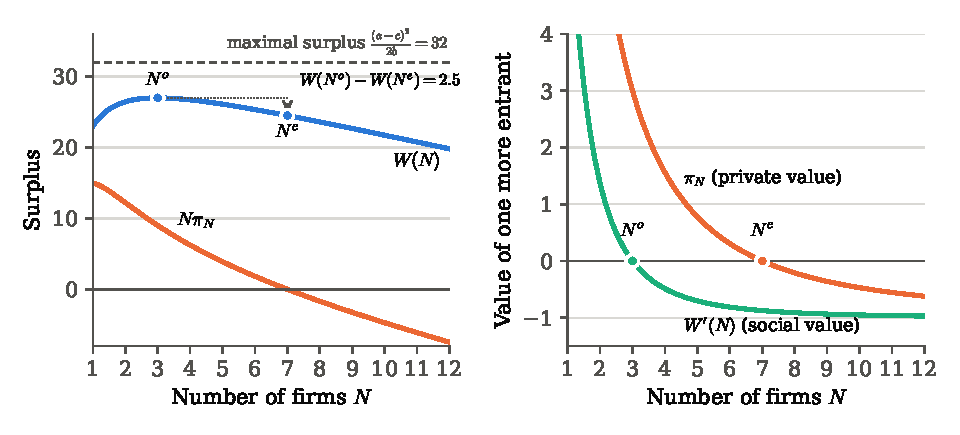
\includegraphics[width=\linewidth]{figures/ch02/entry_welfare.pdf}
\caption{Excess entry in the linear Cournot market with $a - c = 8$, $b = 1$ and $F = 1$. In the left panel, total
surplus $W(N)$ peaks at $N^o = 3$, while industry profit $N\pi_N$ reaches zero at $N^e = 7$. The welfare gap
$W(3) - W(7) = 27 - 24.5 = 2.5$ is 7.8 percent of the maximal surplus of 32. In the right panel, the private value
of entry $\pi_N$ exceeds its social value $W'(N)$ by the business-stealing term in \eqref{eq:02-mw-wprime}.}
\label{fig:02-entry}
\end{figure}

\begin{example}[Free entry into a cartel]\label{ex:02-mw-cartel}
Example~2 of \citet{MankiwWhinston1986} keeps the linear market but lets the entrants form a cartel. Total output is
the monopoly output $Q^m = \frac{a - c}{2b}$ for every $N$, and $q_N = \frac{Q^m}{N}$. Entry now steals business
one for one, since $N\frac{\dd q_N}{\dd N} = -\frac{Q^m}{N} = -q_N$. Using $P^m - c = \frac{a - c}{2}$ in
\eqref{eq:02-mw-wprime},
\begin{equation*}
W'(N) = \pi_N - (P^m - c)\, q_N = \left[(P^m - c)\, q_N - F\right] - (P^m - c)\, q_N = -F .
\end{equation*}
Each extra firm adds nothing but a set-up cost, so the optimum has one firm whenever the market should be served. Free
entry instead continues until $\pi_N = \frac{(a - c)^2}{4bN} - F = 0$, that is, until
$N^m = \frac{(a - c)^2}{4bF}$. Total set-up costs $N^m F = \frac{(a - c)^2}{4b}$ then equal the monopoly profit. The
whole monopoly rent is dissipated in duplicated set-up costs, as in the rent-seeking argument of
\citet{Posner1975} (see \cref{sec:02-welfare}). Welfare falls to the consumer surplus at the monopoly price,
$\frac{(a - c)^2}{8b}$, while one firm would give $\frac{3(a - c)^2}{8b} - F$. As $F \to 0$ the loss tends to
$\frac{(a - c)^2}{4b}$, half of the maximal surplus \citep[n.~10]{MankiwWhinston1986}.
\end{example}

\subsection{The integer constraint}\label{sec:02-mw-integer}

Treating $N$ as continuous is convenient but can mislead. In the cartel example, monopoly profit is
$\frac{(a - c)^2}{4b} - F$, and a monopoly is socially worth having when $\frac{3(a - c)^2}{8b} - F \ge 0$. When
$\frac{(a - c)^2}{4bF} \in [\frac{2}{3}, 1)$ the second condition holds and the first fails. No firm enters, although
one firm is optimal \citep[p.~53]{MankiwWhinston1986}. A monopolist captures only part of the surplus its entry
creates, so entry can be too low. With integers, the cartel example has excess entry only when
$\frac{(a - c)^2}{4bF} \ge 2$ \citep[n.~11]{MankiwWhinston1986}. The next result bounds the shortfall in general.

\begin{proposition}[At most one firm too few]\label{prop:02-mw-integer}
Suppose (E1) to (E3) of \cref{ass:02-mw} hold, with $N$ restricted to the integers and $N^o$ the integer maximizer of
$W$. Then $N^e \ge N^o - 1$ \citep[Proposition~2]{MankiwWhinston1986}.
\end{proposition}

\begin{proof}
The result is trivial when $N^o \le 1$, so let $N^o \ge 2$ and write $Q_N = N q_N$ and $n = N^o$. The proof follows
the appendix of \citet[p.~58]{MankiwWhinston1986}. It first shows that $\pi_{n - 1} \ge 0$ and then that $\pi_N$ is
nonincreasing in $N$.

\emph{Step 1.} Optimality of $n$ implies $W(n) \ge W(n - 1)$. By \eqref{eq:02-mw-welfare} this reads
\begin{equation*}
\int_{Q_{n-1}}^{Q_n} P(x)\, \dd x - n\, C(q_n) + (n - 1)\, C(q_{n-1}) \ge F .
\end{equation*}

\emph{Step 2.} Write $\pi_{n-1} = P(Q_{n-1})\, q_{n-1} - C(q_{n-1}) - F$ and replace $F$ by the larger quantity on
the left of Step~1:
\begin{equation*}
\pi_{n-1} \ge P(Q_{n-1})\, q_{n-1} - \int_{Q_{n-1}}^{Q_n} P(x)\, \dd x + n\left[C(q_n) - C(q_{n-1})\right].
\end{equation*}

\emph{Step 3.} Because $P$ is decreasing and $Q_n > Q_{n-1}$ by (E1), the integral is at most
$P(Q_{n-1})(Q_n - Q_{n-1})$. Moreover $q_{n-1} - (Q_n - Q_{n-1}) = n\, q_{n-1} - n\, q_n$. Hence
\begin{equation*}
\pi_{n-1} \ge n\, P(Q_{n-1})\left(q_{n-1} - q_n\right) + n\left[C(q_n) - C(q_{n-1})\right].
\end{equation*}

\emph{Step 4.} Convexity of $C$ gives, for any two outputs $q$ and $q'$,
\begin{equation}\label{eq:02-convex-ineq}
C(q') - C(q) \ge C'(q)\,(q' - q) .
\end{equation}
Applying it with $q = q_{n-1}$ and $q' = q_n$ yields
\begin{equation*}
\pi_{n-1} \ge n\left[P(Q_{n-1}) - C'(q_{n-1})\right]\left(q_{n-1} - q_n\right) \ge 0 ,
\end{equation*}
where the first factor is nonnegative by (E3) and the second is positive by (E2).

\emph{Step 5.} For any $N$, the fact that $P(Q_N) \le P(Q_{N-1})$ gives
\begin{align*}
\pi_N - \pi_{N-1} &= \left[P(Q_N)\, q_N - C(q_N)\right] - \left[P(Q_{N-1})\, q_{N-1} - C(q_{N-1})\right] \\
&\le P(Q_{N-1})\left(q_N - q_{N-1}\right) - \left[C(q_N) - C(q_{N-1})\right] \\
&\le \left[P(Q_{N-1}) - C'(q_{N-1})\right]\left(q_N - q_{N-1}\right) \le 0 ,
\end{align*}
using \eqref{eq:02-convex-ineq} in the third line and (E2), (E3) for the sign.

\emph{Step 6.} By \eqref{eq:02-free-entry}, $\pi_{N^e + 1} < 0$, and by Step~5 every $N \ge N^e + 1$ has negative
profit. Step~4 shows that $\pi_{n-1} \ge 0$, so $n - 1 < N^e + 1$. Since both sides are integers, $n - 1 \le N^e$.
\end{proof}

A shortfall of one firm can still be costly. In Example~3 of \citet{MankiwWhinston1986}, one firm in the linear market
acts as a monopolist, while two firms play Bertrand and price at $c$. A duopolist earns $-F$, so at most one firm
enters. A monopoly enters when $F \le \frac{(a - c)^2}{4b}$. Welfare is $W(1) = \frac{3(a - c)^2}{8b} - F$ with one
firm and $W(2) = \frac{(a - c)^2}{2b} - 2F$ with two. Duopoly is better when $F \le \frac{(a - c)^2}{8b}$. The loss
from one firm too few is then $\frac{(a - c)^2}{8b} - F$, which approaches 25 percent of the maximal surplus as
$F \to 0$ \citep[pp.~53--54]{MankiwWhinston1986}. Business stealing holds here only weakly, since
$q_1 = q_2 = \frac{a - c}{2b}$.

\subsection{Product diversity}\label{sec:02-diversity}

With differentiated products a new entrant also adds variety. Following \citet{Spence1976},
\citet[pp.~54--55]{MankiwWhinston1986} write gross consumer benefit as $G\left(\sum_i \psi(q_i)\right)$, where
$q_i$ is firm $i$'s output. The subutility $\psi$ satisfies $\psi(0) = 0$, $\psi' > 0$ and $\psi'' \le 0$, and $G$
satisfies $G' > 0$ and $G'' < 0$. These assumptions say that consumers like variety and that the products are
substitutes. (The symbols $G$ and $\psi$ are local to this subsection.) With $N$ symmetric firms the planner solves
\begin{equation}\label{eq:02-diversity-W}
\max_N\; W(N) = G\left(N \psi(q_N)\right) - N C(q_N) - N F .
\end{equation}
Consumer optimization sets each firm's price equal to the marginal benefit of its output,
$p_N = G'\left(N\psi(q_N)\right)\psi'(q_N)$, so per-firm profit is
\begin{equation*}
\pi_N = G'\left(N\psi(q_N)\right)\psi'(q_N)\, q_N - C(q_N) - F .
\end{equation*}
Differentiating \eqref{eq:02-diversity-W}, with arguments suppressed, gives
\begin{equation*}
W'(N) = G'\left[N\psi'\frac{\dd q_N}{\dd N} + \psi\right] - C(q_N) - N C'\frac{\dd q_N}{\dd N} - F .
\end{equation*}
Adding and subtracting $G'\psi' q_N$ and regrouping yields the generalization of \eqref{eq:02-mw-wprime}:
\begin{equation}\label{eq:02-diversity-wprime}
W'(N) = \pi_N + N\left[G'\psi' - C'\right]\frac{\dd q_N}{\dd N} + G'\left[\psi(q_N) - \psi'(q_N)\, q_N\right] .
\end{equation}
The second term is the business-stealing wedge, now with price $G'\psi'$. It is negative when price exceeds marginal
cost and entry contracts incumbents. The third term is new. $G'\psi$ is the entrant's contribution to gross surplus,
while $G'\psi' q_N$ is its revenue. Concavity and $\psi(0) = 0$ imply $\psi(q) \ge \psi'(q)\, q$, so the third term is
nonnegative. It is the surplus from added variety that the entrant cannot appropriate. In the homogeneous case
$\psi(q) = q$ and $G(Q) = \int_0^Q P(x)\,\dd x$, the third term vanishes and \eqref{eq:02-mw-wprime} returns.

The two wedges push in opposite directions, so the sign of the entry bias is ambiguous. With $\psi(q) = q^{\varsigma}$
for some $\varsigma < 1$ and firms that take $G'$ as given, the diversity term dominates for every $N$ and entry is
too low \citep{Spence1976}. \citet{DixitStiglitz1977} also show that monopolistic
competition can produce too little entry. Replacing Spence's price taking with conjectural variations can reverse
this result \citep{KoenkerPerry1981}. \citet[p.~55]{MankiwWhinston1986} also give a functional form, with a quadratic
$\psi$ and linear cost, in which business stealing dominates and entry is excessive. Demand substitutability is
neither necessary nor sufficient for business stealing \citep[n.~14]{MankiwWhinston1986}. Spatial models give further
examples. In the circular city with linear transport costs, the free-entry number of firms is twice the optimum
\citep[sec.~7.1.2]{Tirole1988}, and \cref{ch:diffprod} develops these location models.

\subsection{Small set-up costs}\label{sec:02-small-F}

\Cref{tab:02-mw} shows the loss from excess entry falling as set-up costs fall. The cartel example shows that this
need not happen. There the loss tends to half of the maximal surplus as $F \to 0$. Mankiw and Whinston isolate what
separates the two cases. Write $W^o_F$ and $W^e_F$ for welfare at the optimum and under free entry when the set-up
cost is $F$, and $p_N = G'\left(N\psi(q_N)\right)\psi'(q_N)$ for the price.

\begin{proposition}[Vanishing loss as set-up costs vanish]\label{prop:02-mw-small}
Suppose (E2) holds and, in addition, (i) $p_N$ is decreasing in $N$ and $\lim_{N\to\infty} N\psi(q_N) < \infty$,
(ii) $p_N - C'(q_N) > 0$ for all $N$, and (iii) $\lim_{N\to\infty}\left[p_N - C'(q_N)\right] = 0$. Then
$\lim_{F\to 0}\left(W^o_F - W^e_F\right) = 0$ \citep[Proposition~3]{MankiwWhinston1986}.
\end{proposition}

\begin{proof}[Proof sketch]
Let $W^\infty = \lim_{N\to\infty}\left[G\left(N\psi(q_N)\right) - N C(q_N)\right]$. This limit is finite and is the
best welfare attainable with no set-up cost, so $W^\infty \ge W^o_F \ge W^e_F$ for every $F$. It suffices to show
that $W^e_F \to W^\infty$. First, $N^e_F \to \infty$ as $F \to 0$. Otherwise, for small enough $F$ one more firm
would earn $(p_N - \frac{C(q_N)}{q_N})\, q_N - F \ge (p_N - C'(q_N))\, q_N - F > 0$, using $C(q) \le C'(q)\, q$ for
convex $C$ with $C(0) = 0$. Given $N^e_F \to \infty$, welfare under free entry converges to $W^\infty$ exactly when
total set-up costs $N^e_F F$ vanish. The zero-profit condition bounds them:
\begin{equation*}
N^e F \le \left[p_{N^e} - \frac{C(q_{N^e})}{q_{N^e}}\right] N^e q_{N^e} .
\end{equation*}
As $N^e \to \infty$, per-firm output tends to zero because $N\psi(q_N)$ stays bounded. Average cost and marginal cost
then both tend to $C'(0)$, so the bracket tends to $\lim\left[p_N - C'(q_N)\right] = 0$ by (iii). Total output
$N^e q_{N^e}$ stays bounded, so $N^e F \to 0$.
\end{proof}

Two assumptions do the work. Price must exceed marginal cost for every finite $N$, which is (ii), and approach it
as $N$ grows, which is (iii). Mankiw and Whinston assume both and leave the post-entry game unspecified.
\citet{Novshek1980} derives (iii) for Cournot competition as efficient scale shrinks. Linear Cournot satisfies
(ii) and (iii), which is why the losses in \cref{tab:02-mw} decline. The cartel example violates (iii), since price
stays at the monopoly level for every $N$. Example~3 satisfies (iii) but violates (ii). Price falls to marginal
cost already at $N = 2$, so a second entrant cannot cover its set-up cost. The loss from having one firm too few
therefore persists as $F \to 0$ \citep[p.~57]{MankiwWhinston1986}. The upshot is that regulating entry matters most in markets
with large set-up costs and imperfect competition. It matters little where entry is cheap and competition is close
to perfect.

\subsection{Margins and concentration under fixed and free entry}\label{sec:02-LH}

Free entry changes how margins and concentration move together. With a fixed number of firms, concentration is a
primitive and the Lerner index responds to it. With free entry, both are equilibrium outcomes driven by the same
primitives. The linear market makes the point precisely, using the four columns of \cref{tab:02-linear-cournot}.

\begin{example}[Lerner index and Herfindahl index in four regimes]\label{ex:02-LH}
Let $P = a - bQ$, marginal cost $c$, set-up cost $F$, and $r \equiv \sqrt{bF}$.

\emph{Cournot with fixed $N$.} Here $L = \frac{a - c}{a + Nc}$ and $\HHI = \frac{1}{N}$. Substituting
$N = \frac{1}{\HHI}$ and multiplying numerator and denominator by $\HHI$,
\begin{equation}\label{eq:02-LH-cournot}
L = \frac{(a - c)\,\HHI}{a\,\HHI + c}, \qquad
\frac{\dd L}{\dd \HHI} = \frac{c(a - c)}{(a\,\HHI + c)^2} > 0, \qquad
\frac{\dd^2 L}{\dd \HHI^2} = -\frac{2ac(a - c)}{(a\,\HHI + c)^3} < 0 .
\end{equation}
The relation is increasing and concave. It is causal, since $N$ is set from outside.

\emph{Cournot with free entry.} From \cref{ex:02-free-entry-linear}, $L = \frac{r}{c + r}$ and
$\HHI = \frac{r}{a - c - r}$. These points lie on the curve \eqref{eq:02-LH-cournot} for the same $(a, c)$, because
\begin{equation*}
\frac{(a - c)\frac{r}{a - c - r}}{\frac{a\, r}{a - c - r} + c} = \frac{(a - c)\, r}{a\, r + c(a - c - r)}
= \frac{(a - c)\, r}{(a - c)(r + c)} = \frac{r}{c + r} .
\end{equation*}
Both indices are now endogenous. A higher $F$ or $b$ raises $r$ and moves the industry up along the curve. A higher
$a$ lowers $\HHI$ and leaves $L$ unchanged. A higher $c$ lowers $L$ and raises $\HHI$.

\emph{Collusion with fixed $N$.} Here $L = \frac{a - c}{a + c}$ for every $N$, while $\HHI = \frac{1}{N}$. The
Lerner index does not depend on concentration at all.

\emph{Collusion with free entry.} By \cref{ex:02-mw-cartel}, $N^m = \frac{(a - c)^2}{4bF}$, so
$\HHI = \frac{4bF}{(a - c)^2}$ and $L = \frac{a - c}{a + c}$. A higher $F$ or $b$ raises $\HHI$ only. A higher $a$
raises $L$ and lowers $\HHI$, and a higher $c$ does the reverse.

Finally, collusion attracts more entrants than Cournot competition. With $x = \frac{a - c}{\sqrt{bF}}$,
\eqref{eq:02-Ne-linear} gives $N^e = x - 1$, while $N^m = \frac{x^2}{4}$. Then
\begin{equation*}
N^m - N^e = \frac{x^2}{4} - x + 1 = \left(\frac{x}{2} - 1\right)^2 \ge 0 .
\end{equation*}
\end{example}

\begin{table}[htbp]
\centering
\begin{threeparttable}
\caption{Comparative statics of the Lerner and Herfindahl indices in the linear market}
\label{tab:02-LH-cases}
\renewcommand{\arraystretch}{1.6}
\begin{tabular}{@{}lcccccc@{}}
\toprule
 & & & \multicolumn{4}{c}{Effect of a higher primitive on $(L, \HHI)$} \\
\cmidrule(l){4-7}
Regime & $L$ & $\HHI$ & $F$ & $b$ & $a$ & $c$ \\
\midrule
Cournot, fixed $N$ & $\frac{a - c}{a + Nc}$ & $\frac{1}{N}$ & $(0, 0)$ & $(0, 0)$ & $(+, 0)$ & $(-, 0)$ \\
Cournot, free entry & $\frac{\sqrt{bF}}{c + \sqrt{bF}}$ & $\frac{\sqrt{bF}}{a - c - \sqrt{bF}}$ & $(+, +)$ &
  $(+, +)$ & $(0, -)$ & $(-, +)$ \\
Collusion, fixed $N$ & $\frac{a - c}{a + c}$ & $\frac{1}{N}$ & $(0, 0)$ & $(0, 0)$ & $(+, 0)$ & $(-, 0)$ \\
Collusion, free entry & $\frac{a - c}{a + c}$ & $\frac{4bF}{(a - c)^2}$ & $(0, +)$ & $(0, +)$ & $(+, -)$ &
  $(-, +)$ \\
\bottomrule
\end{tabular}
\begin{tablenotes}\footnotesize
\item Notes: $P = a - bQ$, constant marginal cost $c$, set-up cost $F$. Each cell gives the signs of the effects on
$L$ and $\HHI$. Under free entry the number of firms is treated as continuous.
\end{tablenotes}
\end{threeparttable}
\end{table}

\begin{figure}[htbp]
\centering
\begin{tikzpicture}
\begin{axis}[
  width=0.86\linewidth, height=0.62\linewidth,
  xmin=0, xmax=1.02, ymin=0.25, ymax=0.78,
  xlabel={Herfindahl index $\HHI$}, ylabel={Lerner index $L$},
  xtick={0,0.25,0.5,0.75,1}, ytick={0.3,0.4,0.5,0.6,0.7},
  axis lines=left, every axis plot/.append style={thick},
  clip=false]
  \addplot[domain=0.1:1, samples=120, blue!70!black] {8*x/(10*x+2)};
  \node[blue!70!black, anchor=north west, font=\small, align=left] at (axis cs:0.62,0.585)
    {Cournot\\ $a = 10$, $c = 2$};
  \addplot[domain=0.075:1, samples=120, blue!70!black, dashed, thin] {10*x/(12*x+2)};
  \node[blue!70!black, anchor=west, font=\footnotesize] at (axis cs:1.0,0.725) {$a = 12$};
  \addplot[domain=0.17:1, samples=120, blue!70!black, dotted, thin] {7*x/(10*x+3)};
  \node[blue!70!black, anchor=west, font=\footnotesize] at (axis cs:1.0,0.538) {$c = 3$};
  \addplot[domain=0:1, samples=2, orange!85!black] {2/3};
  \node[orange!85!black, anchor=south west, font=\small] at (axis cs:0.40,0.672)
    {collusion, $L = \frac{a - c}{a + c}$};
  \addplot[only marks, mark=*, mark size=2pt, black] coordinates {(0.3333,0.5)};
  \node[anchor=north, font=\footnotesize] at (axis cs:0.3333,0.488) {$A$};
  \draw[-{Stealth[length=2.2mm]}, thick] (axis cs:0.3333,0.5) -- (axis cs:0.4545,0.5556);
  \node[anchor=north west, font=\footnotesize] at (axis cs:0.462,0.545) {$F$ or $b$ up};
  \draw[-{Stealth[length=2.2mm]}, thick] (axis cs:0.3333,0.5) -- (axis cs:0.25,0.5);
  \draw[thin, gray] (axis cs:0.245,0.503) -- (axis cs:0.16,0.56);
  \node[anchor=south, font=\footnotesize] at (axis cs:0.15,0.56) {$a$ up};
  \draw[-{Stealth[length=2.2mm]}, thick] (axis cs:0.3333,0.5) -- (axis cs:0.4,0.4);
  \node[anchor=north west, font=\footnotesize] at (axis cs:0.40,0.40) {$c$ up};
  \addplot[only marks, mark=square*, mark size=2pt, orange!85!black] coordinates {(0.25,0.6667)};
  \draw[densely dashed, gray] (axis cs:0.3333,0.5) -- (axis cs:0.25,0.6667);
  \node[anchor=south east, font=\footnotesize] at (axis cs:0.25,0.6667) {$B$};
\end{axis}
\end{tikzpicture}
\caption{Lerner index against Herfindahl index in the linear market with $a = 10$, $c = 2$, $b = 1$. The solid curve
is $L = \frac{8\,\HHI}{10\,\HHI + 2}$, the Cournot relation \eqref{eq:02-LH-cournot}. Point $A$ is the Cournot
free-entry outcome with $F = 4$ ($N^e = 3$). Arrows show the free-entry responses to higher $F$ or $b$ (along the
curve), higher $a$ (onto the dashed curve) and higher $c$ (onto the dotted curve). Point $B$ is the collusive
free-entry outcome with the same primitives ($N^m = 4$). It has a higher margin and lower concentration than $A$.}
\label{fig:02-LH}
\end{figure}

The lesson is a theoretical one. The sign of a cross-industry relation between margins and concentration depends on
which primitive varies across industries and on how firms compete. Points $A$ and $B$ in \cref{fig:02-LH} share every
primitive and differ only in conduct. A sample that mixes Cournot and collusive industries pairs high margins with low
concentration and can produce a flat or negative slope. A regression of $L$ on $\HHI$ across industries therefore has
no structural interpretation without a model of entry and conduct. \Cref{ch:intro} discusses these regressions, and
\cref{app:problems} works through the full problem.

\section{Bertrand competition and capacity constraints}\label{sec:02-bertrand}

Cournot firms choose quantities and let the market set the price. Many firms instead post prices and serve whatever
demand arrives. This section studies price competition with a homogeneous good. Its main result is stark: two firms
suffice for the competitive price. We then show how capacity constraints undo the result and when quantity
competition is the better description.

\subsection{Price competition with a homogeneous good}\label{sec:02-bertrand-homog}

\begin{definition}[Bertrand game with a homogeneous good]\label{def:02-bertrand}
There are $N \ge 2$ firms with constant marginal costs $c_i$ and no capacity limits. Market demand $Q(p)$ is
continuous and nonincreasing. Firms choose prices $p_i \ge 0$ simultaneously. Let $p_{\min} = \min_i p_i$ and let
$k$ be the number of firms that charge $p_{\min}$. Each of these firms sells $\frac{Q(p_{\min})}{k}$, and every other
firm sells nothing. Firm $i$ earns $(p_i - c_i)\, q_i$, and each firm must serve all demand at its posted price.
\end{definition}

These are the stage-game rules used for repeated price competition in \cref{ch:collusion-theory}. In the static game
with symmetric costs the tie rule (equal split) does not affect equilibrium outcomes. It matters with asymmetric
costs and for the collusive shares in the repeated game.

\begin{proposition}[The Bertrand paradox]\label{prop:02-bertrand}
Suppose all firms have the same marginal cost $c$ and $Q(c) > 0$. Then a pure-strategy Nash equilibrium exists. In
every pure-strategy Nash equilibrium $p_{\min} = c$, at least two firms charge $c$, and every firm earns zero profit.
\end{proposition}

\begin{proof}
Take any price profile and consider four exhaustive cases.

\emph{Case 1, $p_{\min} < c$.} The firms charging $p_{\min}$ sell $\frac{Q(p_{\min})}{k} \ge \frac{Q(c)}{k} > 0$ at a
loss. Any of them can raise its price above $p_{\min}$ and sell nothing, earning zero. So the profile is not an
equilibrium.

\emph{Case 2, $p_{\min} > c$ and $Q(p_{\min}) > 0$.} If $k \ge 2$, a firm at $p_{\min}$ earns
$(p_{\min} - c)\frac{Q(p_{\min})}{k}$. By cutting its price to $p_{\min} - \eta$ it serves the whole market and earns
at least $(p_{\min} - \eta - c)\, Q(p_{\min})$, because $Q$ is nonincreasing. For small $\eta > 0$ this exceeds its
current profit, since $k \ge 2$. If $k = 1$, any other firm earns zero and can charge a price $p' \in (c, p_{\min})$,
earning $(p' - c)\, Q(p') \ge (p' - c)\, Q(p_{\min}) > 0$. Either way someone deviates.

\emph{Case 3, $p_{\min} > c$ and $Q(p_{\min}) = 0$.} Every firm earns zero. By continuity of $Q$ and $Q(c) > 0$ there
is a price $p'$ slightly above $c$ with $Q(p') > 0$, and $p' < p_{\min}$ because $Q$ is nonincreasing. A firm that
deviates to $p'$ earns $(p' - c)\, Q(p') > 0$.

\emph{Case 4, $p_{\min} = c$.} If only one firm charges $c$, it earns zero. Let $p_{(2)} > c$ be the second-lowest
price. By continuity it can raise its price to some $p' \in (c, p_{(2)})$ with $Q(p') > 0$ and earn a positive
profit. So at least two firms must charge $c$. In that case every firm earns zero. A firm that raises its price sells
nothing and still earns zero, and a firm that cuts below $c$ makes a loss. No deviation is profitable, so any profile
with at least two firms at $c$ is an equilibrium.
\end{proof}

The paradox is the contrast with \cref{sec:02-cournot}. A symmetric Cournot duopoly has industry conduct
$\theta = \frac{1}{2}$ (\cref{sec:02-conduct}). A Bertrand duopoly prices at
marginal cost, so $\theta = 0$ even with two firms. The number of firms alone does not pin down margins. The mode of
competition matters just as much. Two firms suffice for competitive pricing only under stark assumptions: identical
products, constant marginal cost, no capacity limits, and a single round of play. Each assumption points to a
resolution. Capacity constraints are the subject of \cref{sec:02-capacity}. Product differentiation is the subject of
\cref{ch:diffprod}. Repeated interaction is previewed in \cref{sec:02-collusion} and developed in
\cref{ch:collusion-theory}.

\casehead{Asymmetric costs} Let $c_1 < c_2 \le c_j$ for all $j \ge 3$, and let $p^m(c_1)$ be the monopoly price of a
firm with cost $c_1$. If $p^m(c_1) \le c_2$, firm 1's cost advantage is \emph{drastic}. It charges $p^m(c_1)$ and
serves the market, while rivals price at or above their costs. If $p^m(c_1) > c_2$, firm 1 wants to price just below
$c_2$. With continuous prices and an equal split of ties, there is no largest price below $c_2$, so a pure
equilibrium fails to exist. Two standard modifications restore one. If ties go to the low-cost firm, then
$p_1 = p_2 = c_2$ is an equilibrium in which firm 1 serves the market and earns $(c_2 - c_1)\, Q(c_2)$. If prices lie
on a grid with step $\iota$ and $c_2$ on the grid, then $p_1 = c_2$ and $p_2 = c_2 + \iota$ is an equilibrium for
small $\iota$. In this equilibrium firm 2 avoids the weakly dominated choice of pricing at its own cost. Either way, the market price
is
\begin{equation*}
P = \min\left\{c_2,\; p^m(c_1)\right\}.
\end{equation*}
The efficient firm earns a margin limited by its rival's cost, with Lerner index $\frac{c_2 - c_1}{c_2}$ in the
non-drastic case. Measured against the producing firm's marginal cost $c_1$, this market shows a positive conduct
parameter $\theta = \varepsilon\frac{c_2 - c_1}{c_2}$, although firms play Bertrand. A positive estimated $\theta$ can
thus reflect cost asymmetry as well as softer conduct.

\begin{remark}[Increasing marginal cost]\label{rem:02-bertrand-convex}
Let $N$ symmetric firms have a strictly convex cost $C(q)$ with $C(0) = 0$, and keep the obligation to serve all
demand at the posted price. Consider a common price $p$ at which each firm sells $\frac{Q(p)}{N}$ and earns
$u(p) = \frac{p\, Q(p)}{N} - C\left(\frac{Q(p)}{N}\right)$. Raising the price sells nothing and earns $C(0) = 0$.
Undercutting slightly serves the whole market and earns close to $v(p) = p\, Q(p) - C(Q(p))$. For prices below the
level that maximizes $v$, the common price $p$ is an equilibrium if and only if
\begin{equation*}
u(p) \ge 0 \qquad\text{and}\qquad u(p) \ge v(p) .
\end{equation*}
Both conditions hold strictly at the competitive price $p^*$, defined by $p^* = C'\left(\frac{Q(p^*)}{N}\right)$.
Write $q^* = \frac{Q(p^*)}{N}$. The first holds because average cost is below marginal cost for strictly convex $C$
with $C(0) = 0$. For the second, apply \eqref{eq:02-convex-ineq} strictly:
\begin{equation*}
v(p^*) - u(p^*) = p^*\left(Nq^* - q^*\right) - \left[C(Nq^*) - C(q^*)\right]
< p^*\left(Nq^* - q^*\right) - C'(q^*)\left(Nq^* - q^*\right) = 0 .
\end{equation*}
By continuity both inequalities also hold in an interval of prices around $p^*$. Pure equilibria therefore exist and
form a continuum, with prices above and below the competitive level \citep{Dastidar1995}.

Without the obligation to serve, a firm sells only what it wishes at its posted price. Firm $i$'s \emph{competitive
supply} $S_i(p)$ is defined by $p = C_i'(S_i(p))$, and a firm never sells more than $S_i(p)$. The natural candidate is
then the competitive price $p^*$, with $S_1(p^*) + S_2(p^*) = Q(p^*)$ in a duopoly. Suppose rationing is
\emph{efficient}, so that the consumers with the highest willingness to pay are served first (\cref{def:02-rationing}
below). Then $p^*$ is not an equilibrium \citep[sec.~5.3.2]{Tirole1988}. Let firm 2 charge $p^*$ and sell
$q_2^* = S_2(p^*)$, and write $q_1^* = S_1(p^*)$. If firm 1 raises its price to some $p$ slightly above $p^*$, it
serves the residual demand $Q(p) - q_2^*$, which is below $S_1(p)$. Its profit is
$p\,[Q(p) - q_2^*] - C_1(Q(p) - q_2^*)$, whose derivative at $p^*$ is
\begin{equation*}
Q(p^*) - q_2^* + \bigl[p^* - C_1'(q_1^*)\bigr]Q'(p^*) = q_1^* > 0 ,
\end{equation*}
because $Q(p^*) - q_2^* = q_1^*$ and $p^* = C_1'(q_1^*)$. The units lost were sold at marginal cost, so the loss is of
second order, while the higher price on the remaining units is a first-order gain. Equilibria then generally involve
mixed strategies, and both firms' prices exceed the competitive price. Decreasing returns therefore soften price
competition, and the capacity constraint of \cref{sec:02-capacity} is the extreme case.
\end{remark}

\begin{remark}[Strategic substitutes and complements]\label{rem:02-strategic}
\citet[p.~489]{BulowGeanakoplosKlemperer1985} call a lower price or a higher quantity a ``more aggressive'' move.
They classify competition by how a rival's aggressive move changes the \emph{marginal} profit of the firm's own
aggressive move. Choices are strategic substitutes when the rival's aggressive move lowers this marginal profit and
\emph{strategic complements} when it raises it.
Equivalently, best responses slope down under substitutes and up under complements. \Cref{sec:02-cournot-br}
showed that quantities are substitutes in Cournot competition under \cref{ass:02-cournot}. With differentiated products and linear demand
$q_i = d_0 - d_1 p_i + d_2 p_j$, where $0 < d_2 < d_1$, profit $(p_i - c)\, q_i$ gives
$\frac{\partial^2 \pi_i}{\partial p_i \partial p_j} = d_2 > 0$. A lower $p_j$ therefore lowers
$\frac{\partial \pi_i}{\partial p_i}$, which raises the marginal profit of cutting $p_i$. Prices are complements, and
the best response $p_i = \frac{d_0 + d_1 c + d_2 p_j}{2 d_1}$ slopes up, with slope
$\frac{d_2}{2d_1} \in \left(0, \frac{1}{2}\right)$ as \eqref{eq:02-reaction-slope} predicts. \citet[sec.~11.2]{Tirole1988}
uses the same linear demand, $q_i = 1 - bp_i + dp_j$, to illustrate Nash equilibrium in prices. The classification
depends on demand as well as on the strategic variable. \citet[p.~490]{BulowGeanakoplosKlemperer1985} note that
Cournot competition with constant-elasticity demand may yield strategic complements. Our derivation from
\cref{rem:02-c2} gives the threshold. With constant-elasticity demand, $P' + q_i P'' = P'\left(1 - s_i \chi\right)$ with
curvature $\chi = 1 + \frac{1}{\varepsilon}$. The cross-partial is therefore positive, and quantities are complements,
when $s_i\left(1 + \frac{1}{\varepsilon}\right) > 1$.
\end{remark}

\subsection{Capacity constraints and rationing}\label{sec:02-capacity}

\citet{Edgeworth1925}, in an article first published in Italian in 1897, observed that the Bertrand outcome collapses
once firms cannot serve the whole market \citep[sec.~5.2.1]{Tirole1988}. Let two
firms have constant marginal cost $c$ up to capacities $k_1$ and $k_2$, beyond which they cannot produce. Suppose
$k_2 < Q(c)$ and both firms charge $c$. If firm 1 raises its price slightly, firm 2 cannot serve everyone who wants to
buy at $c$. Some consumers turn to firm 1 at the higher price, and firm 1 earns a positive margin on them. So
$p_1 = p_2 = c$ is no longer an equilibrium. When capacities are intermediate, no pure-strategy equilibrium exists at
all. Firms undercut each other until one prefers to raise its price and serve the leftover demand, and the cycle
repeats. The equilibrium of the static game is in mixed strategies \citep{LevitanShubik1972}. What a high-price firm
can sell depends on which consumers the low-price firm serves.

\begin{definition}[Rationing rules]\label{def:02-rationing}
Let firm 1 charge $p_1 < p_2$ with capacity $k_1 < Q(p_1)$. A \emph{rationing rule} gives the residual demand
$Q_2(p_2)$ left for firm 2.
\begin{enumerate}[label=(\roman*)]
\item Under \emph{efficient rationing}, firm 1 serves the consumers with the highest willingness to pay first. Firm 2
  faces
  \begin{equation*}
  Q_2(p_2) = \max\left\{0,\; Q(p_2) - k_1\right\}.
  \end{equation*}
\item Under \emph{proportional rationing}, every consumer who wants to buy at $p_1$ is equally likely to be served
  by firm 1. The fraction $\frac{k_1}{Q(p_1)}$ of them is served. The unserved consumers are a random sample, so a
  fraction $1 - \frac{k_1}{Q(p_1)}$ of the demand at any price remains:
  \begin{equation*}
  Q_2(p_2) = Q(p_2)\left(1 - \frac{k_1}{Q(p_1)}\right).
  \end{equation*}
\end{enumerate}
\end{definition}

Efficient rationing maximizes consumer surplus given the capacities, since the units go to those who value them most.
It also leaves the high-price firm the least demand. Proportional residual demand is larger because
\begin{equation*}
Q(p_2)\left(1 - \frac{k_1}{Q(p_1)}\right) \ge Q(p_2) - k_1
\quad\Longleftrightarrow\quad
\frac{Q(p_2)}{Q(p_1)}\, k_1 \le k_1 ,
\end{equation*}
which holds because $Q(p_2) \le Q(p_1)$. \Cref{fig:02-rationing} draws both residual demands. Efficient rationing
shifts demand inward in parallel by $k_1$. Proportional rationing rotates it around the choke price.

\citet[sec.~5.3.1]{Tirole1988} interprets the two rules. Efficient rationing is the outcome if consumers can resell the
good to each other at no cost, since such arbitrage moves the units to those who value them most. It also arises when
identical consumers with downward-sloping demands are each rationed equally. Proportional rationing, also called
randomized rationing, gives every consumer the same chance of being served. It leaves some low-value consumers with the
bargain, and the high-price firm prefers it because its residual demand is larger. Many other rules are possible.
Suppose rationing works through queues, and the most eager buyers also have the highest value of time. Then the least
eager buyers may end up with the low price. In applications the rationing rule stands in for a model of consumer
behavior, and the right rule depends on the market.

\begin{figure}[htbp]
\centering
\begin{tikzpicture}[scale=0.62, >=Stealth]
  \draw[->] (0,0) -- (10.2,0) node[below] {$q$};
  \draw[->] (0,0) -- (0,10.2) node[left] {$p$};
  \draw[very thick, black] (0,9) -- (9,0) node[pos=0.85, above right] {$Q(p)$};
  \node[below] at (9,0) {$Q(0)$};
  \draw[dashed, gray] (0,3) -- (6,3);
  \node[left] at (0,3) {$p_1$};
  \draw[very thick, orange!85!black] (0,3) -- (3,3);
  \draw[decorate, decoration={brace, amplitude=5pt, mirror}] (0,2.8) -- (3,2.8)
    node[midway, below=5pt] {$k_1$};
  \draw[dotted] (6,3) -- (6,0) node[below] {$Q(p_1)$};
  \draw[very thick, blue!70!black] (3,3) -- (0,6);
  \draw[very thick, blue!70!black, dashed] (3,3) -- (0,9);
  \node[blue!70!black, anchor=west, font=\small] (eff) at (6.2,6.4) {$Q(p) - k_1$ (efficient)};
  \draw[thin, gray] (eff.west) -- (1.0,5.0);
  \node[blue!70!black, anchor=west, font=\small] (prop) at (5.2,8.6)
    {$Q(p)\left(1 - \frac{k_1}{Q(p_1)}\right)$ (proportional)};
  \draw[thin, gray] (prop.west) -- (1.2,6.6);
  \fill (3,3) circle (2.5pt);
  \node[anchor=north west, font=\small] at (3,2.9) {$Q(p_1) - k_1$};
  \node[left] at (0,9) {$\bar p$};
  \node[left] at (0,6) {$P(k_1)$};
\end{tikzpicture}
\caption{Residual demand of the high-price firm. Firm 1 charges $p_1$ and sells its capacity $k_1 < Q(p_1)$. Under
efficient rationing firm 2 faces $Q(p) - k_1$ for $p > p_1$ (solid), a parallel inward shift of demand. Under
proportional rationing it faces $Q(p)\left(1 - \frac{k_1}{Q(p_1)}\right)$ (dashed), which rotates demand around the
choke price $\bar p$. Drawn for $Q(p) = 9 - p$, $p_1 = 3$ and $k_1 = 3$.}
\label{fig:02-rationing}
\end{figure}

\citet{KrepsScheinkman1983} turn Edgeworth's problem into a foundation for Cournot competition. Firms first choose
capacities and then, having observed them, compete in prices. Write $r_\gamma(k)$ for the Cournot best response of a
firm with constant marginal cost $\gamma$ to rival output $k$.

\begin{proposition}[Capacity commitment yields Cournot outcomes]\label{prop:02-ks}
Consider a duopoly in which firms first build capacities $k_i$ at constant unit cost $c_k > 0$, then observe them
and set prices. Production costs $c \ge 0$ per unit up to capacity. Suppose inverse demand is concave and residual
demand follows efficient rationing. Then the game has a unique subgame-perfect equilibrium outcome. It coincides with
the Cournot outcome of the one-stage game with marginal cost $c + c_k$ \citep{KrepsScheinkman1983}.
\end{proposition}

A linear example shows the mechanism before the general argument \citep[sec.~5.3.2.1]{Tirole1988}.

\begin{example}[Capacity-constrained price competition with linear demand]\label{ex:02-ks-linear}
Let $Q(p) = 1 - p$, let capacity cost $c_k \in \left[\frac{3}{4}, 1\right]$ per unit, and let production cost nothing
up to capacity. Rationing is efficient. No firm builds more than $\frac{1}{3}$. In the pricing stage a firm cannot
earn more than the monopoly revenue $\max_p p(1 - p) = \frac{1}{4}$. Its net profit is therefore at most
$\frac{1}{4} - c_kk_i$, which is negative for $k_i > \frac{1}{3}$ because $c_k \ge \frac{3}{4}$.

Take capacities in $\left[0, \frac{1}{3}\right]$. We claim that both firms charging the market-clearing price
$p^* = 1 - k_1 - k_2$ is an equilibrium of the pricing stage. A lower price gains nothing, since firm $i$ already
sells its whole capacity at $p^*$. At a higher price $p > p^*$, firm $i$ sells the residual demand
$q = 1 - p - k_j < k_i$. Its revenue $pq$ is then $(1 - q - k_j)q$, the Cournot objective against rival output
$k_j$. This objective is concave in $q$, and its derivative at $q = k_i$ is $1 - 2k_i - k_j \ge 0$. Revenue therefore
rises on $[0, k_i]$, and the best choice is $q = k_i$, that is, the price $p^*$. The reduced-form profits after the
pricing stage are
\begin{equation}\label{eq:02-ks-linear}
  \Pi_i(k_i, k_j) = (1 - k_i - k_j)\,k_i - c_k k_i ,
\end{equation}
the profits net of capacity cost. This is Tirole's eq.~(5.3). His eq.~(5.2) is the same profit gross of capacity
cost, $(1 - k_i - k_j)k_i$. The net profits are exactly the Cournot profits for outputs $k_i$ and marginal cost
$c_k$. The capacity stage is therefore a Cournot game. Its equilibrium has $k_1 = k_2 = \frac{1 - c_k}{3} \le
\frac{1}{12}$ and price $p^* = \frac{1 + 2c_k}{3}$.
\end{example}

\casehead{Two foundations for Cournot} \citet[sec.~5.3.4]{Tirole1988} separates two results. The pricing stage has
an \emph{exact Cournot reduced form} when, at every pair of capacities that can arise, its equilibrium profits equal
the Cournot profits with quantities read as capacities. The two-stage game has a \emph{Cournot outcome} when its
subgame-perfect capacities and price coincide with the Cournot equilibrium. The first result implies the second,
because the capacity stage is then the Cournot game. It also covers variants, such as capacities chosen in sequence.
\Cref{ex:02-ks-linear} has the exact reduced form. \Cref{prop:02-ks} claims only the Cournot outcome. In its general
setting the reduced form is Cournot for small capacities only, and large capacities lead to mixed equilibria with
other payoffs.

\casehead{The pricing stage} To simplify, set the production cost to $c = 0$, as \citet[sec.~5.7.2.1]{Tirole1988}
does, and assume $k_1 + k_2 < Q(0)$. Write $r(k) = r_0(k)$ for the output that maximizes $qP(q + k)$. Inverse demand
is concave, so this objective is strictly concave in $q$. By \cref{lem:02-cournot-br}, $r$ is single-valued and
decreasing, with slope in $(-1, 0)$.

\begin{lemma}[Pure equilibria clear the market]\label{lem:02-ks1}
In a pure-strategy equilibrium of the pricing stage, $p_1 = p_2 = P(k_1 + k_2)$, and both firms sell their
capacities \citep[sec.~5.7.2.1, Lemma~1]{Tirole1988}.
\end{lemma}

\begin{proof}
Suppose first that $p_1 = p_2 = p > P(k_1 + k_2)$. Demand at $p$ is below total capacity, so some firm $i$ sells less
than $k_i$. By charging $p - \eta$ it would serve the whole market and sell more, which raises its profit for small
$\eta > 0$. Suppose next that $p_1 = p_2 = p < P(k_1 + k_2)$. Both firms ration their customers, and either one could
raise its price slightly and still sell its capacity. Finally, suppose $p_i < p_j$. If firm $i$ is capacity
constrained, it can raise its price slightly and still sell $k_i$. Otherwise it serves all demand at $p_i$, and
optimality requires $p_i$ to be its unconstrained monopoly price, which is positive. Firm $j$ then sells nothing, and
it could earn a positive profit by charging $p_i - \eta$. Each case contradicts equilibrium.
\end{proof}

\begin{lemma}[Pure equilibria lie below the reaction curves]\label{lem:02-ks2}
In a pure-strategy equilibrium of the pricing stage, no firm charges less than $P(k_j + r(k_j))$
\citep[sec.~5.7.2.1, Lemma~2]{Tirole1988}. Consequently, a pure-strategy equilibrium exists if and only if
$k_i \le r(k_j)$ for both firms, and it is then the market-clearing price $P(k_1 + k_2)$.
\end{lemma}

\begin{proof}
By \cref{lem:02-ks1}, both firms charge $p = P(k_1 + k_2)$ in a pure equilibrium. Suppose $p < P(k_j + r(k_j))$,
which means $k_i > r(k_j)$. Let firm $i$ deviate to $p' = P(k_j + r(k_j)) > p$. Firm $j$ still sells $k_j$ at $p$.
Under efficient rationing firm $i$ faces the residual demand $Q(p') - k_j = r(k_j) < k_i$, which it can serve. Its
revenue becomes $r(k_j)P(r(k_j) + k_j)$, the largest Cournot revenue against $k_j$. This exceeds $k_iP(k_i + k_j)$,
because $r(k_j)$ is the unique maximizer and $k_i \ne r(k_j)$. The deviation is profitable, a contradiction. Hence a
pure equilibrium requires $k_i \le r(k_j)$ for both firms.

Conversely, let $k_i \le r(k_j)$ for both firms, and let both charge $p^* = P(k_1 + k_2)$. A price cut does not help
firm $i$, because it already sells its whole capacity. At a price $p > p^*$, efficient rationing leaves firm $i$ the
residual demand $q = Q(p) - k_j < k_i$. Choosing $p$ is therefore the same as choosing an output $q < k_i$ sold at
$P(q + k_j)$. The revenue $qP(q + k_j)$ is the Cournot objective against $k_j$. It is concave in $q$ and peaks at
$r(k_j) \ge k_i$, so it rises on $[0, k_i]$. The best choice is $q = k_i$, which means charging $p^*$.
\end{proof}

In the pure-strategy region the reduced form is exactly Cournot. The Cournot capacities with capacity cost $c_k$ lie
in this region. Indeed $r_\gamma(k)$ solves $P(q + k) + q P'(q + k) = \gamma$, whose left side falls in $q$, so the
best response falls when $\gamma$ rises. Hence $r_{c_k}(k) < r(k)$ at every $k$ where $r_{c_k}(k) > 0$.

\begin{lemma}[The larger firm earns its Stackelberg-follower profit]\label{lem:02-ks3}
Suppose $k_i > r(k_j)$ for at least one firm, so that the pricing stage has only mixed-strategy equilibria. Then the
firm with the larger capacity, say firm $i$, earns
\begin{equation}\label{eq:02-ks-follower}
  F(k_j) = r(k_j)\,P\bigl(k_j + r(k_j)\bigr)
\end{equation}
in every equilibrium \citep[sec.~5.7.2.1, Lemma~3]{Tirole1988}.
\end{lemma}

\begin{proof}[Proof sketch]
In a mixed equilibrium every price in a firm's support yields the same expected profit (\cref{sec:02-nash}).
Consider the top of the support of the larger firm, and suppose that at this price it is undercut with probability
one. It then sells along the efficient residual demand $Q(p) - k_j$, so choosing the price is the same as choosing a
quantity against $k_j$. Optimality at the top of the support requires the quantity $r(k_j)$, which yields $F(k_j)$.
Indifference across the support makes $F(k_j)$ the firm's equilibrium profit. \citet{KrepsScheinkman1983} show that
it is indeed the larger firm whose highest price is undercut for sure, and they construct the equilibrium
distributions. Tirole sketches the argument.
\end{proof}

The name comes from the Stackelberg follower, which chooses its best response to the leader's output
(\cref{ex:02-stackelberg}). The key feature of \eqref{eq:02-ks-follower} is that $F(k_j)$ does not depend on the
larger firm's own capacity. Capacity beyond the pure region only adds cost.

\casehead{The capacity stage} Let $q^{**}$ be the symmetric Cournot output with marginal cost $c_k$, which maximizes
$q\,[P(q + q^{**}) - c_k]$. We show that $k_1 = k_2 = q^{**}$ is an equilibrium of the capacity stage
\citep[sec.~5.7.2.2]{Tirole1988}. Let firm $i$ choose $q^{**}$, and consider firm $j$'s choice $k$. In the pricing
stage the capacity cost is sunk, so each firm wants to sell more than it would if capacity were still to be paid
for. In particular $r(q^{**}) > q^{**}$.
\begin{itemize}
  \item Let $k \le r(q^{**})$. The capacities then lie in the pure region. When $k \le q^{**}$ this holds because
  $r(k) \ge r(q^{**}) > q^{**}$. When $q^{**} < k \le r(q^{**})$, the slope bound $r' > -1$ gives
  $r(k) > r(q^{**}) - (k - q^{**}) \ge q^{**}$. Firm $j$ therefore earns the Cournot profit $k\,[P(k + q^{**}) -
  c_k]$, which is at most $q^{**}[P(2q^{**}) - c_k]$ by the definition of $q^{**}$.
  \item Let $k > r(q^{**})$. The pricing stage is then in the mixed region, and firm $j$ has the larger capacity. By
  \cref{lem:02-ks3} its net profit is $F(q^{**}) - c_k k$. Since $k > r(q^{**})$,
  \[
    F(q^{**}) - c_k k < r(q^{**})\bigl[P\bigl(r(q^{**}) + q^{**}\bigr) - c_k\bigr] \le q^{**}\bigl[P(2q^{**}) -
    c_k\bigr] ,
  \]
  where the last step again uses the definition of $q^{**}$.
\end{itemize}
No deviation pays. The Cournot capacities therefore form an equilibrium of the capacity stage, and the price is
$P(2q^{**})$. Proving that this outcome is unique takes more work \citep{KrepsScheinkman1983}.

\casehead{Rationing and the cost of capacity} The result also depends on the rationing rule when capacity is cheap.
\citet{DavidsonDeneckere1986} study rules other than efficient rationing \citep[secs.~5.3.4 and 5.7.2.3]{Tirole1988}.
For virtually any such rule, the Cournot outcome cannot be an equilibrium of the two-stage game when the capacity
cost is small. A first-order calculation at the Cournot point shows why. Let both firms hold the Cournot
capacities $q^{**}$ and charge $p^{**} = P(2q^{**})$, now with production cost $c \ge 0$. Let $Q_2(p_2)$ be firm 2's
residual demand for $p_2$ just above $p^{**}$, with $Q_2(p^{**}) = q^{**}$. The capacity cost is sunk, so a small
price increase changes firm 2's profit at the rate
\[
  A = q^{**} + (p^{**} - c)\,Q_2'(p^{**}) .
\]
The Cournot first-order condition with marginal cost $c + c_k$ gives $p^{**} - c - c_k = -q^{**}P'(2q^{**}) =
\frac{q^{**}}{\lvert Q'(p^{**})\rvert}$. Substituting,
\begin{equation}\label{eq:02-dd}
  A = q^{**}\left(1 - \frac{\lvert Q_2'(p^{**})\rvert}{\lvert Q'(p^{**})\rvert}\right)
      - c_k\,\lvert Q_2'(p^{**})\rvert .
\end{equation}
Efficient rationing has $Q_2' = Q'$, so $A = -c_k\lvert Q'(p^{**})\rvert < 0$, and a price increase does not pay. A
rule whose residual demand responds less to price than market demand, $\lvert Q_2'(p^{**})\rvert < \lvert
Q'(p^{**})\rvert$, makes the first term positive. For small enough $c_k$ the rate $A$ is then positive. Firm 2 gains
by raising its price above the market-clearing level, and the Cournot capacities do not lead to the Cournot price.
With price on the vertical axis, as in \cref{fig:02-rationing}, such a residual demand is steeper than market demand.
Proportional rationing is such a rule. By \cref{def:02-rationing}, it
gives $Q_2(p) = Q(p)\bigl(1 - \frac{q^{**}}{Q(p^{**})}\bigr) = \frac{Q(p)}{2}$. Hence $Q_2' = \frac{Q'}{2}$ and
$A = \frac{1}{2}\bigl(q^{**} - c_k\lvert Q'(p^{**})\rvert\bigr)$.

Costly capacity restores the Cournot form. Keep the demand $Q(p) = 1 - p$ and the zero production cost of
\cref{ex:02-ks-linear}, but let $c_k \in (0, 1)$. Then $q^{**} = \frac{1 - c_k}{3}$ and $\lvert Q'\rvert = 1$, so
under proportional rationing $A > 0$ if and only if $c_k < \frac{1}{4}$.
Equivalently, the Cournot price $p^{**} = \frac{1 + 2c_k}{3}$ then lies below the monopoly price $\frac{1}{2}$. A firm
that raises its price faces a scaled-down copy of market demand, $\frac{Q(p)}{2}$. Its best higher price is therefore
the monopoly price whenever that price exceeds $p^{**}$. For $c_k \ge \frac{1}{4}$ the market-clearing price is at
least $\frac{1}{2}$, and no firm wants to raise it. More generally, \citet[Exercise~5.2]{Tirole1988} shows that with
this demand, proportional rationing and capacities below $\frac{1}{4}$, both firms charge the market-clearing price.
The reduced form is then exactly Cournot again. The result is due to \citet{Beckmann1967} for proportional rationing
and to \citet{LevitanShubik1972} for efficient rationing. The Kreps-Scheinkman foundation is thus a statement about
timing and about the cost of capacity. It does not license Cournot competition in every market with capacity choice.

\casehead{Further caveats} \citet[sec.~5.3.4]{Tirole1988} stresses that both foundations rest on strong
assumptions. They are more likely to hold when the capacity cost is high. A large gap between ex ante and ex post
costs then makes firms willing to dump their capacity on the market ex post. Price setting must be the last stage,
with no later rounds of price competition and no product differentiation. Folding the two stages into a one-stage
quantity game can also discard what actions reveal, for example when firms infer rivals' costs from their behavior.
Finally, most firms do not face rigid capacity limits. Their cost curves rise beyond some output without the inverted
L shape, so there is often no capacity level that gives the Cournot quantity a meaning.

The construction also needs rivals to observe capacities before they set prices. If capacities are not observed,
the game is equivalent to one in which quantities and prices are chosen simultaneously
\citep[sec.~5.7.2.4]{Tirole1988}. \citet{Gertner1985} studies this simultaneous game and allows increasing or
decreasing returns. We follow Tirole and take a constant marginal cost $c$. In this game a firm produces before it
learns whether it sells. No pure-strategy equilibrium exists, and the unique equilibrium is in
mixed strategies. The symmetric equilibrium is easy to verify. Let $\bar p$ be the choke price, with $Q(\bar p) = 0$.
Each firm draws its price from $F(p) = 1 - \frac{c}{p}$ on $[c, \bar p)$, with the remaining probability
$\frac{c}{\bar p}$ at $\bar p$, and produces $Q(p)$ when it charges $p$. The rival never rations its customers, so
a firm that charges $p$ sells $Q(p)$ when its rival charges more, which happens with probability $1 - F(p)$. It pays
for its output in any case. Its expected profit is
\[
  \bigl[(1 - F(p))\,p - c\bigr]\,Q(p) = \Bigl(\frac{c}{p}\,p - c\Bigr)Q(p) = 0
\]
at every price in the support, and prices below $c$ lose money \citep[Exercise~5.9]{Tirole1988}. Expected profit is
zero, as in Bertrand, but the expected price exceeds $c$, as in Cournot. A firm cannot commit not to flood the
market, and this competitive pressure drives profits down.

\subsection{Bertrand or Cournot?}\label{sec:02-bertrand-vs-cournot}

The choice between the two models is a choice about what firms commit to before they compete. Bertrand competition
fits markets where capacity is ample or quickly adjusted and firms post prices that they cannot easily revise.
Differentiated-goods markets are the main case, and most empirical work on them assumes Nash equilibrium in prices
(\cref{ch:diffprod}). Cournot competition fits markets where output or capacity is committed before prices form, as
in commodities produced in advance or capacity-constrained industries. Both models impose conduct rather than
measuring it. Which description fits a given industry is an empirical question, and this motivates estimating
conduct directly (\cref{sec:02-conduct} and \cref{ch:conduct}).

\citet[sec.~5.6]{Tirole1988} draws the same lesson from cost structure. Firms almost always set prices, so the two
models are not rival accounts of one market. They describe markets with different technologies. Bertrand is the
better approximation when marginal cost is fairly flat. Cournot is the better approximation when marginal cost
rises sharply, as it does at a capacity limit. Quantity competition is then best read as competition in scale: each
firm's choice of scale fixes its cost function and so the conditions of later price competition. A capacity is one
such choice, and other investments that shape the cost curve play the same role. Tirole also warns that the
capacity justification must be checked model by model, for the reasons given in \cref{sec:02-capacity}.

\begin{remark}[Supply function equilibria]\label{rem:02-sfe}
In some markets firms commit to entire supply schedules. In an electricity pool, for example, generators submit
schedules before demand is known. Let firm $i$ commit to a supply function $S_i(p)$, and let the price clear the market,
$Q(p) = \sum_j S_j(p)$. Given its rivals' schedules, firm $i$ faces residual demand $Q(p) - S_{-i}(p)$, with
$S_{-i} = \sum_{j \ne i} S_j$. For each realization of demand it chooses the best point on this curve. The first-order
condition is
\begin{equation*}
q_i = \left(p - C_i'(q_i)\right)\left[S_{-i}'(p) - Q'(p)\right].
\end{equation*}
Rearranging, and writing $e_{-i} = S_{-i}'(p)\frac{p}{S_{-i}}$ for the elasticity of rivals' supply and
$S_{-i} = (1 - s_i)Q$, gives
\begin{equation*}
\frac{p - C_i'(q_i)}{p} = \frac{s_i}{\varepsilon + (1 - s_i)\, e_{-i}} .
\end{equation*}
Flat rival schedules ($e_{-i} = 0$) give the Cournot rule $\frac{s_i}{\varepsilon}$. Infinitely elastic schedules
give price equal to marginal cost, as in Bertrand. The same formula describes a dominant firm facing a price-taking
fringe, \eqref{eq:02-dominant-lerner} in \cref{ex:02-dominant}. \citet{KlempererMeyer1989} show that, without uncertainty, many supply function
equilibria exist, with outcomes between the competitive and Cournot outcomes. Demand uncertainty narrows the set, and
with unbounded uncertainty the equilibrium is unique. \citet{GreenNewbery1992} apply the model to the British
electricity spot market, which \cref{ch:conduct} studies with the data of \citet{Wolfram1999}.
\end{remark}

Price competition can also be studied dynamically. Consider a duopoly in which firms take turns setting prices and
condition only on the rival's current price. A \emph{Markov perfect equilibrium} is a subgame-perfect equilibrium in
which each firm's price depends only on the payoff-relevant state, here the rival's current price. In this game such
equilibria take two forms \citep[pp.~571--572]{MaskinTirole1988}. In a \emph{kinked demand curve} equilibrium the
price settles at a focal level, because each firm expects a price cut to be matched and a price rise to go unmatched.
In an \emph{Edgeworth cycle} firms undercut each other in small steps until the price war becomes too costly. Then
one firm raises its price, the other follows, and the undercutting starts again. In every such equilibrium profit
stays bounded away from the Bertrand level. Such cycles appear in retail gasoline markets
(\cref{ch:collusion-evidence}).

\section{Conduct: conjectural variations and the conduct parameter}\label{sec:02-conduct}

Monopoly, Cournot and Bertrand each deliver one pricing rule. Empirical work needs a single equation that nests them,
so that the data can speak about which one holds. This section develops that equation, the supply relation with a
conduct parameter $\theta$. It shows how firm behavior aggregates into an industry $\theta$, lists the values that
standard models imply, and discusses what an estimated $\theta$ can and cannot mean. Estimation and identification
are the subject of \cref{ch:conduct}.

\subsection{The supply relation}\label{sec:02-supply-relation}

Let $P(Q)$ be inverse market demand and $MC$ industry marginal cost. The \emph{supply relation} with \emph{conduct
parameter} $\theta \ge 0$ is
\begin{equation}\label{eq:02-supply-relation}
P = MC - \theta\, Q\, P'(Q) .
\end{equation}
Equivalently, $P + \theta Q P'(Q) = MC$: marginal cost equals a \emph{perceived marginal revenue}. At $\theta = 0$
this is price taking, $P = MC$. At $\theta = 1$ it is the monopoly condition $MR = MC$. Since $P' < 0$, the term
$-\theta Q P'(Q) \ge 0$ is the dollar markup. It equals $\theta$ times the monopoly markup $m = -\frac{Q(p)}{Q'(p)}$
of \eqref{eq:02-dollar-markup}. Relation \eqref{eq:02-supply-relation} is the industry form of Bresnahan's supply
relation \eqref{eq:02-bresnahan-supply}, which \cref{sec:02-infer-mc} stated at the level of firm $i$ and
observation $t$, with $\theta_{it}$ free to vary. Bresnahan calls it a supply relation because, outside perfect
competition, firms have no supply curve that gives output as a function of price alone
\citep[p.~1016, n.~6]{Bresnahan1989}. As there, marginal cost is a function of unknown parameters that are
estimated jointly with $\theta$.

Dividing \eqref{eq:02-supply-relation} by $P$ and using $\varepsilon = -\frac{P}{Q P'(Q)}$ gives the Lerner form:
\begin{equation}\label{eq:02-theta-lerner}
\frac{P - MC}{P} = -\frac{\theta\, Q\, P'(Q)}{P} = \frac{\theta}{\varepsilon}
\qquad\Longleftrightarrow\qquad
\theta = \varepsilon\,\frac{P - MC}{P} .
\end{equation}
The conduct parameter is the \emph{elasticity-adjusted Lerner index}. For $\theta \in [0, 1]$ the Lerner index lies
in $\left[0, \frac{1}{\varepsilon}\right]$, between price taking and the inverse-elasticity rule.

\begin{remark}[Conduct between competition and monopoly]\label{rem:02-theta-bounds}
Under \eqref{eq:02-supply-relation}, $\theta \in [0, 1]$ if and only if
\begin{equation*}
P + Q P'(Q) \le MC \le P ,
\end{equation*}
that is, marginal cost lies between monopoly marginal revenue and price. Indeed $MC = P + \theta Q P'$ with
$QP' < 0$. So $MC \le P$ holds exactly when $\theta \ge 0$, and $MC \ge P + QP'$ holds exactly when $\theta \le 1$.
These inequalities yield bounds on marginal cost without fixing $\theta$, and they hold observation by observation
even when conduct varies. \citet{Rosen2007} builds on this idea to bound marginal cost and markups by set
identification, and \cref{sec:03-bounds} develops the approach.
\end{remark}

\begin{example}[The linear system]\label{ex:02-linear-system}
Let demand and marginal cost be linear,
\begin{align*}
Q_t &= \alpha_0 + \alpha_1 P_t + \alpha_2 Y_t + e_t , \qquad \alpha_1 < 0, \\
MC_t &= \beta_0 + \beta_1 Q_t + \beta_2 W_t + u_t ,
\end{align*}
where $Y_t$ shifts demand, $W_t$ shifts cost, and $e_t$ and $u_t$ are shocks. (In this example only, $\alpha$ and
$\beta$ denote the coefficients of the linear system.) The inverse demand slope is
$P'(Q) = \frac{1}{\alpha_1}$. Substituting it and $MC_t$ into \eqref{eq:02-supply-relation} gives
\begin{align}
P_t &= \beta_0 + \beta_1 Q_t + \beta_2 W_t + u_t - \frac{\theta}{\alpha_1}\, Q_t \notag \\
&= \beta_0 + \left(\beta_1 - \frac{\theta}{\alpha_1}\right) Q_t + \beta_2 W_t + u_t . \label{eq:02-linear-supply}
\end{align}
Conduct and the slope of marginal cost enter only through the composite slope
$\beta_1 - \frac{\theta}{\alpha_1}$. Parallel demand shifts trace out the supply relation and reveal this composite
slope. They cannot tell a competitive industry with rising marginal cost from a monopoly with flatter marginal
cost. \Cref{ch:conduct} shows how demand rotations \citep{Bresnahan1982,Lau1982} break this observational
equivalence.
\end{example}

\subsection{Firm-level conduct and aggregation}\label{sec:02-aggregation}

The supply relation can be derived from firm behavior. Let firm $i$ choose $q_i$ in a homogeneous-good market with
cost $C_i(q_i)$, and suppose it acts as if its rivals' total output responds to its own output with slope
$r_i = \frac{\dd Q_{-i}}{\dd q_i}$. The number $r_i$ is firm $i$'s \emph{conjectural variation}, as in
\cref{prop:01-clarke-davies}. The firm then perceives $\frac{\dd Q}{\dd q_i} = 1 + r_i$, and its perceived marginal
revenue is
\begin{equation*}
\frac{\dd}{\dd q_i}\left[P(Q)\, q_i\right] = P(Q) + q_i P'(Q)\frac{\dd Q}{\dd q_i} = P(Q) + (1 + r_i)\, q_i P'(Q) .
\end{equation*}
Setting it equal to marginal cost gives the firm-level supply relation
\begin{equation}\label{eq:02-firm-foc}
P + \tilde\theta_i\, q_i P'(Q) = C_i'(q_i), \qquad \tilde\theta_i = 1 + r_i .
\end{equation}
We call $\tilde\theta_i$ the \emph{firm-level conduct parameter}. Cournot behavior is $r_i = 0$ and
$\tilde\theta_i = 1$. Price taking is $r_i = -1$ and $\tilde\theta_i = 0$: the firm acts as if rivals offset any
expansion one for one, so price does not move. This is the form of \citet[eqs.~(12) and (14),
pp.~1027--1028]{Bresnahan1989}, whose symbol $r_i$ we adopt. He writes $\theta_{it}$ for $1 + r_i$ and uses the two
forms interchangeably. The literature often uses the same symbol for firm-level and industry-level conduct. We keep
the tilde to separate them.

\begin{proposition}[Aggregation of firm conduct]\label{prop:02-theta-aggregate}
Let each of $N$ firms satisfy \eqref{eq:02-firm-foc}, with shares $s_i = \frac{q_i}{Q}$ and market elasticity
$\varepsilon = -\frac{P}{Q P'(Q)}$. For any weights $\kappa_i \ge 0$ with $\sum_i \kappa_i = 1$, define industry
marginal cost $MC = \sum_i \kappa_i C_i'(q_i)$. Then
\begin{equation}\label{eq:02-theta-aggregate}
\frac{P - MC}{P} = \frac{\theta}{\varepsilon}, \qquad\text{with}\qquad \theta = \sum_{i=1}^N \kappa_i\, s_i\,
\tilde\theta_i ,
\end{equation}
so the industry satisfies the supply relation \eqref{eq:02-supply-relation} with this $\theta$.
\end{proposition}

\begin{proof}
The proof takes five steps.
\begin{enumerate}[label=\arabic*.]
\item Rearrange \eqref{eq:02-firm-foc}: $P = C_i'(q_i) - \tilde\theta_i\, q_i P'(Q)$.
\item Use $-P'(Q) = \frac{P}{\varepsilon Q}$: $P = C_i'(q_i) + \tilde\theta_i\frac{q_i}{Q}\frac{P}{\varepsilon}
  = C_i'(q_i) + \tilde\theta_i\, s_i\frac{P}{\varepsilon}$.
\item Multiply by $\kappa_i$: $\kappa_i P = \kappa_i C_i'(q_i) + \kappa_i s_i \tilde\theta_i\frac{P}{\varepsilon}$.
\item Sum over $i$. Since $\sum_i \kappa_i = 1$, the left side is $P$, and
  $P = \sum_i \kappa_i C_i'(q_i) + \frac{P}{\varepsilon}\sum_i \kappa_i s_i \tilde\theta_i = MC +
  \frac{P}{\varepsilon}\,\theta$.
\item Subtract $MC$ and divide by $P$ to obtain \eqref{eq:02-theta-aggregate}. Multiplying
  $\frac{\theta P}{\varepsilon}$ by $1 = -\frac{\varepsilon Q P'}{P}$ gives $P = MC - \theta Q P'$, which is
  \eqref{eq:02-supply-relation}. \qedhere
\end{enumerate}
\end{proof}

The benchmarks follow at once. Under Cournot conduct ($\tilde\theta_i = 1$), $\theta = \sum_i \kappa_i s_i$. Equal
weights and symmetric firms give $\theta = N \cdot \frac{1}{N}\cdot\frac{1}{N} = \frac{1}{N}$. Share weights
$\kappa_i = s_i$ give $\theta = \HHI$ and industry marginal cost $\bar c = \sum_i s_i c_i$, which is the
Cowling-Waterson relation of \cref{prop:02-cowling-waterson}. Joint profit maximization sets
$P + Q P'(Q) = C_i'(q_i)$ for every active firm. Comparing with \eqref{eq:02-firm-foc} gives
$\tilde\theta_i = \frac{Q}{q_i} = \frac{1}{s_i}$, hence $\theta = \sum_i \kappa_i = 1$. Price taking gives
$\theta = 0$.

Two features of the aggregation deserve emphasis. First, when all firms share the same constant marginal cost $c$,
step~2 of the proof shows that $\tilde\theta_i s_i = \varepsilon\frac{P - c}{P}$ is the same for every firm. The
industry $\theta$ is then independent of the weights. Second, with heterogeneous costs the weights matter, because
noncooperative firms with different costs have different margins (\cref{prop:02-cowling-waterson}). A stable industry
marginal cost curve need not exist, and an industry-level $\theta$ estimated from aggregate data is best read as
average conduct \citep[p.~1030]{Bresnahan1989}. Nothing in oligopoly theory forces all firms to share the same
conduct. \citet[p.~1030]{Bresnahan1989} calls the contrary claim in the literature an error. This is the aggregation
that \citet{Wolfram1999} uses for electricity (\cref{ch:conduct}).

\subsection{The menu of conduct}\label{sec:02-menu}

Each standard oligopoly model implies values of $r_i$, $\tilde\theta_i$ and $\theta$. Two models with leaders need a
derivation.

\begin{example}[Stackelberg leadership]\label{ex:02-stackelberg}
Let $P = a - bQ$ and let all firms have marginal cost $c$. Firm 1 leads, and firms $2, \dots, N$ choose outputs
after observing $q_1$ and play Cournot among themselves. Each follower's first-order condition is
$a - bQ - b q_j = c$. By symmetry the followers produce
\begin{equation*}
q_f = \frac{a - c - b q_1}{bN}, \qquad Q_{-1} = (N - 1)\, q_f = \frac{(N - 1)(a - c - b q_1)}{bN} .
\end{equation*}
The leader's conjecture is correct, $r_1 = \frac{\dd Q_{-1}}{\dd q_1} = -\frac{N - 1}{N}$, so
$\tilde\theta_1 = 1 + r_1 = \frac{1}{N}$. The leader's first-order condition is $a - bQ - \frac{b}{N}q_1 = c$, and total output satisfies
$bQ = b q_1 + b Q_{-1} = \frac{(N - 1)(a - c)}{N} + \frac{b q_1}{N}$. Substituting,
\begin{equation*}
a - c - \frac{(N - 1)(a - c)}{N} - \frac{2 b q_1}{N} = 0
\quad\Longrightarrow\quad q_1 = \frac{a - c}{2b} .
\end{equation*}
Then $q_f = \frac{a - c}{2bN}$, total output is $Q = \frac{(2N - 1)(a - c)}{2bN}$, and $P - c = \frac{a - c}{2N}$.
Industry conduct follows from \eqref{eq:02-supply-relation} with $-QP' = bQ$:
\begin{equation*}
\theta = \frac{P - c}{bQ} = \frac{\frac{a - c}{2N}}{\frac{(2N - 1)(a - c)}{2N}} = \frac{1}{2N - 1} .
\end{equation*}
A duopoly gives $\theta = \frac{1}{3}$, with $P - c = \frac{a - c}{4}$ and $Q = \frac{3(a - c)}{4b}$. Since
$\frac{1}{2N - 1} < \frac{1}{N}$ for $N \ge 2$, leadership is more competitive than Cournot. As a check on
\cref{prop:02-theta-aggregate}, the shares are $s_1 = \frac{N}{2N - 1}$ and $s_f = \frac{1}{2N - 1}$, so
$\tilde\theta_1 s_1 = \tilde\theta_f s_f = \frac{1}{2N - 1}$, as the common-cost case requires.
\end{example}

\citet[p.~1022]{Bresnahan1989} writes the leader's supply relation as \eqref{eq:02-firm-foc} with
$\tilde\theta_1 = 1 + \theta_S$, where $\theta_S$ is the derivative of the followers' total output with respect to
the leader's. In the example $\theta_S = -\frac{N - 1}{N}$.

\begin{example}[Conduct of a dominant firm]\label{ex:02-dominant-conduct}
Return to the dominant firm $d$ of \cref{ex:02-dominant}, which faces a fringe of price takers with aggregate supply
$S(P)$, $S' \ge 0$. Its residual demand is $q_d(P) = Q(P) - S(P)$, with slope $Q'(P) - S'(P)$. Its first-order
condition is
\begin{equation*}
P + \frac{q_d}{Q'(P) - S'(P)} = C_d'(q_d) .
\end{equation*}
Writing this as \eqref{eq:02-firm-foc} with $P'(Q) = \frac{1}{Q'(P)}$ gives
\begin{equation*}
\tilde\theta_d = \frac{Q'(P)}{Q'(P) - S'(P)} = \frac{\varepsilon}{\varepsilon + \varepsilon_f (1 - s_d)} ,
\qquad
v_d = \tilde\theta_d - 1 = -\frac{\varepsilon_f (1 - s_d)}{\varepsilon + \varepsilon_f (1 - s_d)} ,
\end{equation*}
where $\varepsilon_f = S'\frac{P}{S}$ is the fringe supply elasticity and $s_d$ the dominant share. The second form
uses $\frac{S'}{Q'} = -\frac{\varepsilon_f S}{\varepsilon Q} = -\frac{\varepsilon_f (1 - s_d)}{\varepsilon}$. The
dominant firm's Lerner index is $\frac{\tilde\theta_d s_d}{\varepsilon} = \frac{s_d}{\varepsilon +
\varepsilon_f(1 - s_d)}$, which is \eqref{eq:02-dominant-lerner}. Fringe firms have $\tilde\theta = 0$. In
Bresnahan's notation, with $D_1 = P'(Q)$ and $S_1 = S'(P)$, the dominant firm has $\tilde\theta_d = 1 + S_D$ with
$S_D = \frac{D_1 S_1}{1 - D_1 S_1} \in (-1, 0]$ \citep[eqs.~(11) and (11$'$), p.~1023]{Bresnahan1989}.
\citet{Suslow1986} estimates this model for Alcoa in the interwar aluminum market, with recycled aluminum as the
fringe. She finds that Alcoa kept considerable monopoly power because $S_D$ is small
\citep[p.~1023]{Bresnahan1989}.
\end{example}

\begin{remark}[Recycling and durability create a fringe]\label{rem:02-recycling}
A firm that sells a recyclable or durable good creates part of its own competition \citep[sec.~1.5]{Tirole1988}. In
the 1945 antitrust case against the Aluminum Company of America, Alcoa held about 90 percent of the primary aluminum
market. Critics of the decision pointed to an approximately competitive industry that recycled the aluminum Alcoa had
produced. Counting this secondary market, Alcoa's share was only about 64 percent \citep[sec.~1.5.1]{Tirole1988}.

Tirole's model shows how far recycling disciplines the monopolist. Demand in each period is $q_t = Q(p_t)$, with
inverse $P$. A competitive industry recycles the fraction $x(p_{t+1})$ of the previous period's consumption, where
the recycling supply $x$ rises with price, $x' > 0$, and stays below one. The symbol $x$ is local to this remark. The
monopolist supplies the rest at unit cost $c$, so its profit in period $t$ is
\[
  \pi_t = \bigl[P(q_t) - c\bigr]\bigl(q_t - x(P(q_t))\,q_{t-1}\bigr) ,
\]
and it maximizes $\sum_t \delta^t\pi_t$. Output $q_t$ enters $\pi_t$ and, through the recycled stock, $\pi_{t+1}$.
In a stationary state with $q_t = q$, $p = P(q)$ and $x = x(p)$, the first-order condition for $q_t$ is
\[
  P'(q)\,q\,(1 - x) + (p - c)\bigl[1 - x'(p)P'(q)\,q\bigr] - \delta\,(p - c)\,x = 0 .
\]
Solving for the margin and dividing by $p$, with $-\frac{P'(q)q}{p} = \frac{1}{\varepsilon}$, gives
\[
  \frac{p - c}{p} = \frac{1}{\varepsilon}\cdot\frac{1 - x}{1 - \delta x - x'(p)P'(q)\,q} .
\]
This is Tirole's eq.~(1.7) in Lerner form. The term $-x'P'q$ is positive and $\delta < 1$, so the denominator exceeds
$1 - \delta x > 1 - x$. The margin is therefore positive but below the static monopoly margin $\frac{1}{\varepsilon}$.
It approaches zero only when the recycled fraction $x$ approaches one. Tirole judges that this was not the case for
Alcoa, whose demand also grew fast, which keeps the recycled share low. \citet{Suslow1986} estimates a model of this
kind.

Durability has a starker effect. A monopolist that sells a durable good and cannot commit to its future prices
competes with its own later sales, because buyers wait for price cuts. \citet{Coase1972} conjectured that as price
revisions become frequent, the monopolist's profit converges to zero and trade occurs at prices close to marginal
cost. Later work proved the conjecture under suitable conditions \citep[secs.~1.1.3 and 1.5.2]{Tirole1988}.
\end{remark}

\begin{table}[htbp]
\centering
\begin{threeparttable}
\caption{The menu of conduct in a homogeneous-good market}
\label{tab:02-conduct-menu}
\small
\renewcommand{\arraystretch}{1.25}
\begin{tabularx}{\linewidth}{@{}>{\raggedright\arraybackslash}p{0.2\linewidth}cc%
>{\raggedright\arraybackslash}p{0.2\linewidth}>{\raggedright\arraybackslash}X@{}}
\toprule
Model & $r_i$ & $\tilde\theta_i$ & Industry $\theta$ & Source or derivation \\
\midrule
Price taking & $-1$ & $0$ & $0$ & \eqref{eq:02-supply-relation} with $P = MC$ \\
Bertrand, constant cost & $-1$ & $0$ & $0$ for any $N \ge 2$ & \cref{prop:02-bertrand} \\
Cournot & $0$ & $1$ & $\frac{1}{N}$ if symmetric, $\HHI$ if $\kappa_i = s_i$ & \cref{prop:02-theta-aggregate} \\
Symmetric constant conjecture & $r$ & $1 + r$ & $\frac{1 + r}{N}$ & \citet{Iwata1974} \\
Stackelberg leader, $N - 1$ Cournot followers (linear) & $-\frac{N - 1}{N}$ & $\frac{1}{N}$ &
  $\frac{1}{2N - 1}$ & \cref{ex:02-stackelberg} \\
Stackelberg follower & $0$ & $1$ & same as leader row & \cref{ex:02-stackelberg} \\
Dominant firm with price-taking fringe & $\frac{-\varepsilon_f(1 - s_d)}{\varepsilon + \varepsilon_f(1 - s_d)}$ &
  $\frac{\varepsilon}{\varepsilon + \varepsilon_f(1 - s_d)}$ & $\kappa_d\, s_d\,\tilde\theta_d$ &
  \cref{ex:02-dominant-conduct}, \citet{Suslow1986} \\
Joint monopoly or perfect collusion & $\frac{Q_{-i}}{q_i}$ & $\frac{Q}{q_i}$ & $1$ &
  \cref{prop:02-theta-aggregate}, with $r_i = N - 1$ if symmetric \\
Repeated-game collusion & varies & varies & $\theta_t$ high when collusion holds, low in price wars &
  \citet{GreenPorter1984}, \citet{Porter1983} \\
\bottomrule
\end{tabularx}
\begin{tablenotes}\footnotesize
\item Notes: $r_i = \frac{\dd Q_{-i}}{\dd q_i}$ is the conjectural variation, $\tilde\theta_i = 1 + r_i$ the
firm-level conduct parameter in \eqref{eq:02-firm-foc}, and industry $\theta = \sum_i \kappa_i s_i \tilde\theta_i$
(\cref{prop:02-theta-aggregate}). The Bertrand entries are ``as if'' values, since price equals marginal cost. In the
dominant-firm row, $\varepsilon_f$ is the fringe supply elasticity and $s_d$ the dominant share, and fringe firms
have $\tilde\theta = 0$.
\end{tablenotes}
\end{threeparttable}
\end{table}

\Cref{tab:02-conduct-menu} collects the menu. The repeated-game row anticipates \cref{sec:02-collusion} and
\cref{ch:collusion-theory}. In the theory of \citet{GreenPorter1984}, firms observe only the market price and cannot
tell a rival's secret output expansion from low demand. Collusive periods therefore alternate with price wars. Estimated conduct then varies over time.
\citet{Porter1983} estimates such a regime-switching supply relation for a nineteenth-century railroad cartel
(\cref{ch:collusion-evidence}). \Cref{fig:02-perceived-mr} shows the menu at work in the linear market. Each value of
$\theta$ rotates perceived marginal revenue around the demand intercept and selects a different point on the demand
curve.

\begin{figure}[htbp]
\centering
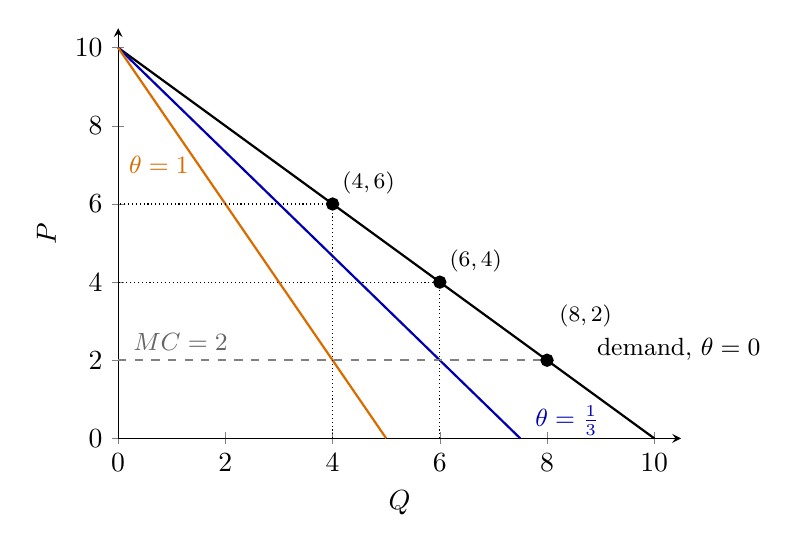
\begin{tikzpicture}
\begin{axis}[
  width=0.72\linewidth, height=0.56\linewidth,
  xmin=0, xmax=10.5, ymin=0, ymax=10.5,
  xlabel={$Q$}, ylabel={$P$},
  xtick={0,2,4,6,8,10}, ytick={0,2,4,6,8,10},
  axis lines=left, every axis plot/.append style={thick}, clip=false]
  \addplot[domain=0:10, samples=2, black] {10 - x};
  \node[anchor=south west, font=\small] at (axis cs:8.75,1.75) {demand, $\theta = 0$};
  \addplot[domain=0:7.5, samples=2, blue!70!black] {10 - (4/3)*x};
  \node[anchor=west, blue!70!black, font=\small] at (axis cs:7.6,0.45) {$\theta = \frac{1}{3}$};
  \addplot[domain=0:5, samples=2, orange!85!black] {10 - 2*x};
  \node[anchor=east, orange!85!black, font=\small] at (axis cs:1.5,7.0) {$\theta = 1$};
  \addplot[domain=0:8, samples=2, gray, dashed] {2};
  \node[anchor=south west, gray!80!black, font=\small] at (axis cs:0.1,2) {$MC = 2$};
  \addplot[only marks, mark=*, mark size=2pt] coordinates {(8,2) (6,4) (4,6)};
  \draw[densely dotted] (axis cs:6,0) -- (axis cs:6,4) -- (axis cs:0,4);
  \draw[densely dotted] (axis cs:4,0) -- (axis cs:4,6) -- (axis cs:0,6);
  \node[anchor=south west, font=\footnotesize] at (axis cs:8.05,2.6) {$(8, 2)$};
  \node[anchor=south west, font=\footnotesize] at (axis cs:6,4) {$(6, 4)$};
  \node[anchor=south west, font=\footnotesize] at (axis cs:4,6) {$(4, 6)$};
\end{axis}
\end{tikzpicture}
\caption{Perceived marginal revenue $10 - (1 + \theta)Q$ for demand $P = 10 - Q$ and $MC = 2$. Price taking
($\theta = 0$, perceived marginal revenue equal to demand) gives $Q = 8$ and $P = 2$. Conduct $\theta = \frac{1}{3}$,
as in a Stackelberg duopoly or a symmetric Cournot triopoly, gives $Q = 6$ and $P = 4$. Monopoly ($\theta = 1$)
gives $Q = 4$ and $P = 6$. In general $Q = \frac{8}{1 + \theta}$.}
\label{fig:02-perceived-mr}
\end{figure}

\subsection{Interpreting the conduct parameter}\label{sec:02-interpret}

\citet[Sec.~2.2]{Bresnahan1989} distinguishes three ways in which empirical work has used $\theta$.

The first takes $\theta$ from a single theory \citep[Sec.~2.2.1]{Bresnahan1989}. \citet{Rosse1970} estimates the
supply relation of monopoly newspapers ($\theta = 1$). His marginal revenue includes the effect of circulation on
advertising prices, and he infers marginal cost from $MR = MC$. Cournot models set $\tilde\theta_i = 1$
\citep[eq.~(6)]{Bresnahan1989}. Stackelberg and dominant-firm models give the leader the values derived above.
Dynamic theories of collusion imply a $\theta$ that switches between regimes, as in \citet{Porter1983}. In all these
cases the theory fixes the value or the pattern of $\theta$ before the data are consulted.

The second approach estimates the supply relations of a few distinct theories and tests them against each other
\citep[Sec.~2.2.2]{Bresnahan1989}. \citet{Bresnahan1987} compares joint-profit pricing with Bertrand pricing in the
automobile industry of the mid-1950s. He finds collusive behavior in some years and Bertrand behavior in 1955
(\cref{ch:discrete}). Bresnahan stresses that this approach differs from estimating a continuous $\theta$ only
econometrically. A continuous $\theta$ leads to nested tests, while a few discrete theories lead to non-nested tests.

The third approach treats $\theta$ as a continuous parameter described as a ``conjectural variation''
\citep[Sec.~2.2.3]{Bresnahan1989}. \citet{Iwata1974} used it to locate the Japanese plate-glass industry between
competition and monopoly. Since $\tilde\theta_i - 1 = r_i$ is an identity, saying what the conjectural variation is
and saying which oligopoly theory fits the data are the same statement \citep[p.~1027]{Bresnahan1989}.

\casehead{The critique of conjectural variations} Taken literally, a conjecture describes how a firm expects rivals
to react to a change in its output. In a simultaneous-move game nobody can react, so any nonzero conjecture is
inconsistent with the game being played. \emph{Consistent conjectures}, which require each conjecture to equal the
actual slope of rivals' responses, were one attempted repair \citep{Bresnahan1981a}. They keep the static framework
and have not become standard. \citet[pp.~1028--1029]{Bresnahan1989} offers a different reading. Collusive conduct
$\tilde\theta_i = N$ would literally mean that each firm expects rivals to match any output change one for one. In
repeated-game models firms produce the collusive output for another reason. They expect a deviation to trigger a
general breakdown of restraint. An estimated $\theta$ therefore describes what firms do. It does not reveal what they
believe would happen after a deviation. If $\theta$ is stable and breakdowns are rare, it measures the average collusiveness of
conduct. It tells us nothing about firms' expectations beyond the fact that they deter deviations
\citep[n.~19]{Bresnahan1989}.

A more basic problem is that an unrestricted $\theta$ explains everything.

\begin{proposition}[Exact fit]\label{prop:02-theta-fit}
Let $(P_{it}, Q_{it})$, with $Q_{it} > 0$, be data on prices and quantities. Take any demand system with slope
$\frac{\partial Q_{it}}{\partial P_{it}} < 0$ at each observation and any marginal cost function, with implied
values $mc_{it}$. Setting
\begin{equation*}
\theta_{it} = \frac{\left(P_{it} - mc_{it}\right)\left|\frac{\partial Q_{it}}{\partial P_{it}}\right|}{Q_{it}}
\end{equation*}
makes the supply relation
\[
P_{it} = mc_{it} + \theta_{it}\frac{Q_{it}}{\left|\frac{\partial Q_{it}}{\partial P_{it}}\right|}
\]
hold exactly at every observation, with no error term. The implied $\theta_{it}$ is nonnegative whenever
$mc_{it} \le P_{it}$.
\end{proposition}

\begin{proof}
Substituting the stated $\theta_{it}$ into the right side of the supply relation gives
\[
mc_{it} + \frac{(P_{it} - mc_{it})\left|\frac{\partial Q_{it}}{\partial P_{it}}\right|}{Q_{it}}
\cdot\frac{Q_{it}}{\left|\frac{\partial Q_{it}}{\partial P_{it}}\right|} = mc_{it} + (P_{it} - mc_{it}) = P_{it} . \qedhere
\]
\end{proof}

The supply relation has empirical content only through restrictions on $\theta$. The usual ones are that $\theta$ is
constant across observations or groups, or that $\theta \in [0, 1]$. Others fix $\theta$ at the value implied by a
specific game, or require deviations of $\theta$ to be uncorrelated with the instruments. Each restriction is an assumption, and
each objection to a conduct study is an objection to one of them. Imposing a functional form on marginal cost does not
help by itself, since the proposition holds for every cost function.

\casehead{The conduct parameter as a specification test} \citet[p.~1031]{Bresnahan1989} credits
\citet{Appelbaum1979} with a useful observation. Setting $\theta = 0$ in \eqref{eq:02-supply-relation} imposes price
taking. Every approach to conduct is therefore a test of price taking against alternatives with market power. A
cautious use of $\theta$ follows. We estimate it freely and test the hypotheses $\theta = 0$,
$\theta = \frac{1}{N}$ and $\theta = 1$, without reading $\hat\theta$ as a deep behavioral parameter. Even this use
requires care. If true conduct varies with demand, as in repeated-game models, an instrumental-variables estimate of a
constant $\theta$ measures how the markup responds to demand shifts. It need not equal average conduct, a point due to
\citet{Corts1999} and developed in \cref{ch:conduct}.

\casehead{Observed marginal cost} When marginal cost can be measured directly, \eqref{eq:02-theta-lerner} delivers
conduct observation by observation, $\theta_t = \varepsilon_t\frac{P_t - MC_t}{P_t}$, once demand is known. A known
cost structure serves a similar purpose. Fixed-proportions technology, for example, pins marginal cost down up to one
or two parameters, which can be estimated jointly with $\theta$. These are the strategies of \citet{Wolfram1999} for
electricity and \citet{GenesoveMullin1998} for sugar refining. Both compare the direct measure with the estimate a
researcher would obtain without cost data (\cref{ch:conduct}).

\subsection{Forward contracts}\label{sec:02-forward}

Contracts signed before the spot market opens change the spot-market incentive to raise price. The case matters for
electricity markets, where most output is often sold forward.

\begin{example}[Cournot with forward sales]\label{ex:02-forward}
Suppose firm $i$ has sold $x_i$ units forward at price $p^f$, before the spot market opens. Its spot-market profit is
\begin{equation*}
P(Q)\left(q_i - x_i\right) + p^f x_i - C_i(q_i) .
\end{equation*}
The forward revenue $p^f x_i$ is fixed, and only the uncontracted output $q_i - x_i$ earns the spot price. The Cournot
first-order condition is
\begin{equation*}
P(Q) + \left(q_i - x_i\right) P'(Q) = C_i'(q_i) .
\end{equation*}
Using $-P' = \frac{P}{\varepsilon Q}$ and dividing by $P$,
\begin{equation}\label{eq:02-forward-lerner}
\frac{P - C_i'(q_i)}{P} = \frac{q_i - x_i}{Q}\cdot\frac{1}{\varepsilon}
= \frac{s_i}{\varepsilon}\left(1 - \frac{x_i}{q_i}\right) .
\end{equation}
In conduct terms, $\tilde\theta_i = 1 - \frac{x_i}{q_i}$. A firm with 80 percent of its output under contract has
one fifth of the Cournot incentive to raise the spot price.
\end{example}

\citet{AllazVila1993} show that firms also have a strategic reason to sell forward. A forward sale commits a firm to
a higher spot output. Since quantities are strategic substitutes, rivals respond by producing less. Every firm has
this incentive, and together they end up in a prisoners' dilemma that lowers prices. In the linear duopoly with
$P = a - bQ$ and cost $c$, suppose arbitrage makes the forward price equal the spot price. The spot stage gives
$q_i = \frac{a - c + 2b x_i - b x_j}{3b}$ and $P - c = \frac{a - c - b(x_1 + x_2)}{3}$. Each firm then chooses $x_i$
to maximize $(P - c)\, q_i$. The first-order condition is $a - c - 4b x_i - b x_j = 0$, so the symmetric solution is
$x_i = \frac{a - c}{5b}$. Spot outputs are $q_i = \frac{2(a - c)}{5b}$, half of output is sold forward, and
$P - c = \frac{a - c}{5}$. Without a forward market, Cournot gives $P - c = \frac{a - c}{3}$. As a check,
\eqref{eq:02-forward-lerner} with $s_i = \frac{1}{2}$ and $\frac{x_i}{q_i} = \frac{1}{2}$ gives
$P - c = \frac{1}{4}\, b Q = \frac{a - c}{5}$. \Cref{ch:conduct} returns to contract cover in the British electricity
market.

\begin{remark}[Very inelastic demand]\label{rem:02-inelastic}
By \cref{prop:02-cowling-waterson}, Cournot firm $i$ has $L_i = \frac{s_i}{\varepsilon}$. With constant-elasticity
demand, an interior equilibrium requires $L_i < 1$, that is, $s_i < \varepsilon$. When market demand is very inelastic, as in electricity, the static
Cournot model predicts no interior equilibrium. Firms would withhold output until a capacity constraint binds. In such
markets prices are held down by something outside the static model. Capacity limits, regulatory threats, forward
contracts and the threat of entry are the usual candidates.
\end{remark}

\subsection{Pricing rules for the Bulow-Pfleiderer family}\label{sec:02-bp-rules}

The supply relation yields closed-form pricing rules for the demand family $Q(p) = B(\bar p - p)^{g}$ of
\cref{ex:02-bp}. With constant marginal cost $c$, the derivation has three steps.

First, compute $q\,P'(q)$. Since $P'(q) = \frac{1}{Q'(p)}$ and $Q'(p) = -gB(\bar p - p)^{g - 1}$,
\begin{equation*}
q\,P'(q) = \frac{Q(p)}{Q'(p)} = \frac{B(\bar p - p)^{g}}{-gB(\bar p - p)^{g - 1}} = -\frac{\bar p - p}{g} .
\end{equation*}
Second, substitute into $p + \theta q P'(q) = c$:
\begin{equation*}
p - \frac{\theta(\bar p - p)}{g} = c
\quad\Longrightarrow\quad
g p + \theta p = g c + \theta \bar p .
\end{equation*}
Third, solve for $p$:
\begin{equation}\label{eq:02-gm-rule}
P(c;\theta) = \frac{\theta\bar p + g c}{g + \theta} .
\end{equation}
Monopoly ($\theta = 1$) gives $P(c;1) = \frac{\bar p + gc}{1 + g}$, the rule of \cref{ex:02-bp}. Price taking
gives $P(c;0) = c$. The rule nests the other families as limits.
\begin{itemize}
\item Linear demand ($g = 1$) gives $P = \frac{\theta\bar p + c}{1 + \theta}$, and quadratic demand ($g = 2$)
  gives $P = \frac{\theta\bar p + 2c}{2 + \theta}$.
\item Constant elasticity ($\bar p = 0$ and $g = -\varepsilon < 0$) gives $P = \frac{gc}{g + \theta}
  = \frac{\varepsilon}{\varepsilon - \theta}\, c$, which requires $\varepsilon > \theta$.
\item In the exponential limit, $g$ and $\bar p$ grow without bound with $\frac{g}{\bar p} = \lambda_s$ fixed. Demand tends to
  $Q \propto e^{-\lambda_s p}$, with constant semi-elasticity $\lambda_s$. Since $\frac{\bar p - p}{g} =
  \frac{1}{\lambda_s} - \frac{p}{g} \to \frac{1}{\lambda_s}$, the rule becomes $P = c + \frac{\theta}{\lambda_s}$, a
  constant dollar markup.
\end{itemize}
The cost slope of \eqref{eq:02-gm-rule} is $\frac{\partial P}{\partial c} = \frac{g}{g + \theta}$, which depends on
conduct and curvature together (\cref{sec:02-passthrough}). The intercept $\frac{\theta\bar p}{g + \theta}$ moves
with the demand parameter $\bar p$. A season in which demand rotates, changing $\bar p$ or $g$, therefore shifts price
by an amount that rises with $\theta$ and vanishes at $\theta = 0$. \citet{GenesoveMullin1998} estimate exactly these rules for sugar refining and
use such a seasonal rotation to identify conduct (\cref{ch:conduct}).

\section{Pass-through}\label{sec:02-passthrough}

The previous sections characterized the level of the markup under each model of competition. Empirical work often
learns more from how prices move than from where they sit. When marginal cost rises by one dollar, by how much does
price rise? The answer, the pass-through rate, links
much of the empirical work in this book. Tax incidence, tests of conduct, the price effects of mergers and the
value of cost savings to consumers all depend on it. This section derives pass-through from the pricing
first-order conditions of \cref{sec:02-monopoly,sec:02-cournot,sec:02-conduct}. Pass-through depends on three
primitives: the curvature of demand, the slope of marginal cost and conduct. One pass-through number cannot
separate them, and much of the section makes that statement precise.

\subsection{Definition and uses}\label{sec:02-pt-uses}

\begin{definition}[Pass-through]\label{def:02-passthrough}
Let the equilibrium price $p$ of a market depend on a cost parameter $c$ that shifts marginal cost one for one.
The \emph{pass-through rate} is $\rho = \frac{\dd p}{\dd c}$. For a \emph{specific tax} $t$, a fixed amount per unit
sold, the pass-through rate is $\rho = \frac{\dd p}{\dd t}$. The \emph{pass-through elasticity} is
$\frac{\dd p}{\dd c}\frac{c}{p} = \rho\frac{c}{p}$. A cost shock is \emph{industry-wide} when it raises the marginal
cost of every firm by the same amount, and \emph{firm-specific} when it raises the marginal cost of one firm
only.
\end{definition}

A specific tax collected from sellers raises their effective marginal cost by $t$. A tax collected from buyers
is equivalent. If buyers pay the tax, demand at the seller price $p_s$ is $Q(p_s + t)$. A monopolist that
chooses $p_s$ to maximize $Q(p_s + t)(p_s - c)$ is choosing the consumer price $p = p_s + t$ to maximize
$Q(p)(p - c - t)$, which is the problem with a tax collected from sellers. The same change of variables works
for every model of conduct in this chapter. The side of the market that legally pays the tax is therefore
irrelevant. The pass-through of a specific tax equals the pass-through of an equal rise in marginal cost.
We use $c$ and $t$ interchangeably when marginal cost is constant.

Pass-through enters applied work in four ways. First, it determines the \emph{incidence} of a tax, the split of
its burden between consumers and producers (\cref{sec:02-pt-incidence}). Second, it governs how shocks to input
prices and exchange rates reach final prices. A pass-through elasticity of import prices below one with respect
to the exchange rate is the ``incomplete pass-through'' of international economics. Third, the pass-through of
an industry-wide cost shifter differs between competition and monopoly, so it can be used to test conduct.
\citet{Sumner1981} built such a test from state cigarette taxes, and \cref{ch:conduct} studies it in depth.
Fourth, merger analysis needs pass-through twice. A merger's cost savings reach consumers only through the
merged firm's pass-through. The upward pricing pressure of a merger is a shift in effective marginal cost, and
pass-through converts it into a price change (\cref{ch:mergers}).

\subsection{Monopoly with constant marginal cost}\label{sec:02-pt-monopoly}

We begin with a single price setter. The same results apply to any firm facing a residual demand curve with
rivals' actions held fixed (\cref{sec:02-residual}).

\begin{assumption}[Monopoly pass-through]\label{ass:02-pt-monopoly}
A monopolist faces demand $Q(p)$, twice continuously differentiable with $Q'(p) < 0$, and has constant marginal
cost $c$. For every $c$ in an open interval $I$, profit $Q(p)(p - c)$ has a unique global maximizer $p^m(c)$,
which is interior, and $p^m$ is continuous on $I$. The maximizer satisfies the first-order condition
\eqref{eq:02-foc-monopoly}, $Q'(p)(p - c) + Q(p) = 0$, and the strict second-order condition $(p - c)Q''(p) +
2Q'(p) < 0$.
\end{assumption}

The strict second-order condition is the nonsingularity condition of the implicit function theorem
(\cref{app:math}). Through each $p^m(c)$ it yields a continuously differentiable local branch of solutions to the
first-order condition, and that branch is locally the only solution. Continuity of $p^m$ keeps the maximizer on
this branch. Hence $p^m(c)$ is continuously differentiable, and its derivative follows from differentiating the
first-order condition. Uniqueness implies continuity when the maximizers lie in a fixed compact set of prices. By
Berge's maximum theorem, a unique maximizer of a continuous objective over a fixed compact set moves continuously
with a parameter. Neither property follows from the local conditions alone. Profit can have two strict global
maximizers at one cost, and the optimal price then jumps from one to the other as $c$ crosses that cost. In such
cases the results below hold on each branch, away from the switching points.

The sign of the derivative is known before we compute it.
\Cref{lem:02-monotone} shows by revealed preference that the monopoly price never falls when $c$ rises, for any
demand curve. Smoothness adds the rate.

\begin{proposition}[Monopoly pass-through]\label{prop:02-pt-monopoly}
Under \cref{ass:02-pt-monopoly}, at $p = p^m(c)$,
\begin{equation}\label{eq:02-pt-monopoly}
\rho = \frac{\dd p^m}{\dd c} = \frac{Q'(p)}{(p - c)Q''(p) + 2Q'(p)} > 0 .
\end{equation}
\end{proposition}

\begin{proof}
Write the first-order condition as an identity in $c$:
\begin{equation*}
Q'\bigl(p(c)\bigr)\bigl(p(c) - c\bigr) + Q\bigl(p(c)\bigr) \equiv 0 .
\end{equation*}
Differentiate each piece with respect to $c$, writing $\rho = p'(c)$:
\begin{align*}
\frac{\dd}{\dd c}\, Q'\bigl(p(c)\bigr) &= Q''(p)\,\rho , \\
\frac{\dd}{\dd c}\, \bigl(p(c) - c\bigr) &= \rho - 1 , \\
\frac{\dd}{\dd c}\, Q\bigl(p(c)\bigr) &= Q'(p)\,\rho .
\end{align*}
The product rule applied to the first term of the identity gives $Q''\rho(p - c) + Q'(\rho - 1)$. Adding the
derivative of the second term,
\begin{equation*}
(p - c)Q''\rho + Q'(\rho - 1) + Q'\rho = 0 .
\end{equation*}
Collect the terms in $\rho$:
\begin{equation*}
\rho\bigl[(p - c)Q'' + 2Q'\bigr] = Q' .
\end{equation*}
Dividing by the bracket gives \eqref{eq:02-pt-monopoly}. The numerator $Q'$ is negative, and the bracket is
negative by the second-order condition, so $\rho > 0$.
\end{proof}

Formula \eqref{eq:02-pt-monopoly} has three equivalent forms. Each one gives a different reading of what drives
pass-through.

\casehead{Log-curvature form}
The first-order condition gives $p - c = -\frac{Q}{Q'}$. Substituting into the denominator of
\eqref{eq:02-pt-monopoly},
\begin{equation*}
(p - c)Q'' + 2Q' = -\frac{QQ''}{Q'} + 2Q' .
\end{equation*}
Dividing the numerator and the denominator of \eqref{eq:02-pt-monopoly} by $Q'$ gives
\begin{equation}\label{eq:02-pt-logcurv}
\rho = \frac{1}{2 - \frac{Q(p)\,Q''(p)}{Q'(p)^2}} .
\end{equation}
The ratio $\frac{QQ''}{(Q')^2}$ is a unit-free measure of the convexity of demand. It is zero for linear demand.

\casehead{Markup-slope form}
Let $m(p) = -\frac{Q(p)}{Q'(p)}$ be the dollar markup that the demand curve supports at price $p$, as in
\eqref{eq:02-dollar-markup}. The first-order condition reads $p - c = m(p)$. Differentiating with respect to $c$
gives $\rho - 1 = m'(p)\rho$, so
\begin{equation}\label{eq:02-pt-markup}
\rho = \frac{1}{1 - m'(p)} .
\end{equation}
The quotient rule gives $m'(p) = -\frac{(Q')^2 - QQ''}{(Q')^2} = -1 + \frac{QQ''}{(Q')^2}$, so
$1 - m'(p) = 2 - \frac{QQ''}{(Q')^2}$, in agreement with \eqref{eq:02-pt-logcurv}. The reciprocal $\frac{1}{m}
= -\frac{Q'}{Q}$ is the semi-elasticity of demand from \cref{sec:02-monopoly-foc}.
When the semi-elasticity rises with price, the supported markup falls ($m' < 0$), and the monopolist absorbs part
of any cost increase. When the semi-elasticity falls with price, the markup rises with price ($m' > 0$), and the
price rises by more than cost.

\casehead{Quantity-space form}
A monopolist choosing output $q$ against inverse demand $P(q)$ sets marginal revenue equal to marginal cost,
$P(q) + qP'(q) = c$. Recall from \cref{rem:02-c2} the curvature of inverse demand,
\begin{equation}\label{eq:02-chi}
\chi(q) = -\frac{qP''(q)}{P'(q)} .
\end{equation}
It is zero for linear inverse demand, positive when inverse demand is convex and negative when it is concave.
Differentiating the marginal-revenue condition with respect to $c$,
\begin{equation*}
\bigl[2P'(q) + qP''(q)\bigr]\frac{\dd q}{\dd c} = 1 .
\end{equation*}
The price moves along the inverse demand curve, so
\begin{equation}\label{eq:02-pt-quantity}
\rho = P'(q)\frac{\dd q}{\dd c} = \frac{P'}{2P' + qP''} = \frac{1}{2 + \frac{qP''}{P'}} = \frac{1}{2 - \chi(q)} .
\end{equation}
The second-order condition in quantity space is $2P' + qP'' < 0$. Dividing by $P' < 0$ shows that it is
equivalent to $\chi < 2$, which again makes $\rho$ positive.

The log-curvature form and the quantity-space form agree because the two curvature measures coincide.

\begin{lemma}[Curvature of direct and inverse demand]\label{lem:02-chi-direct}
Let $P$ be the inverse of a twice differentiable demand function $Q$ with $Q' < 0$. At every point on the demand
curve, $\chi = \frac{QQ''}{(Q')^2}$, and $\frac{\dd^2 \ln Q(p)}{\dd p^2} < 0$ if and only if $\chi < 1$.
\end{lemma}

\begin{proof}
Differentiate the identity $P(Q(p)) = p$ once to get $P'Q' = 1$, so $P' = \frac{1}{Q'}$. Differentiate it again
to get $P''(Q')^2 + P'Q'' = 0$, so $P'' = -\frac{P'Q''}{(Q')^2} = -\frac{Q''}{(Q')^3}$. Then
\begin{equation*}
\chi = -\frac{Q\,P''}{P'} = -Q\cdot\Bigl(-\frac{Q''}{(Q')^3}\Bigr)\cdot Q' = \frac{QQ''}{(Q')^2} .
\end{equation*}
For the second claim, $\frac{\dd^2\ln Q}{\dd p^2} = \frac{\dd}{\dd p}\frac{Q'}{Q} = \frac{QQ'' - (Q')^2}{Q^2}$. This is
negative if and only if $QQ'' < (Q')^2$, that is, if and only if $\chi < 1$.
\end{proof}

\begin{corollary}[\citealp{BulowPfleiderer1983}]\label{cor:02-bulow-pfleiderer}
Under \cref{ass:02-pt-monopoly}, monopoly pass-through at $p^m(c)$ satisfies $\rho < 1$ if demand is strictly
log-concave there, $\rho = 1$ if $\ln Q$ is locally linear, and $\rho > 1$ if demand is strictly log-convex.
Linear demand has $\rho = \frac{1}{2}$.
\end{corollary}

\begin{proof}
By \eqref{eq:02-pt-quantity} and \cref{lem:02-chi-direct}, $\rho = \frac{1}{2 - \chi}$ with $2 - \chi > 0$. So
$\rho < 1$ if and only if $2 - \chi > 1$, that is $\chi < 1$, which is strict log-concavity. The other two cases
follow in the same way. Linear demand has $Q'' = 0$, so $\chi = 0$ and $\rho = \frac{1}{2}$.
\end{proof}

Log-concavity is the same property as a semi-elasticity that rises with price, since
$\frac{\dd^2 \ln Q}{\dd p^2} = \frac{\dd}{\dd p}\frac{Q'}{Q}$. The corollary therefore restates the markup-slope form: a
monopolist passes through less than the full cost increase exactly when higher prices make its customers more
price sensitive at the margin.

\begin{remark}[Pass-through and the distribution of willingness to pay]\label{rem:02-pt-hazard}
Suppose each of $M$ consumers buys one unit if her willingness to pay $v$ exceeds the price, with $v$ drawn from a
distribution $G$ with density $G'$. Demand is $Q(p) = M[1 - G(p)]$, as in \cref{sec:02-monopoly-foc}, and the
supported markup is $m(p) = \frac{1 - G(p)}{G'(p)} = \frac{1}{h(p)}$, where $h = \frac{G'}{1 - G}$ is the hazard rate
of $G$. The
first-order condition reads $p - c = \frac{1}{h(p)}$. Since $m' = -\frac{h'}{h^2}$, \eqref{eq:02-pt-markup} gives
\begin{equation*}
\rho = \frac{1}{1 + \frac{h'(p)}{h(p)^2}} .
\end{equation*}
Pass-through is below one exactly when the hazard rate rises at $p^m$. A uniform distribution on $[0, \bar v]$ has
$h = \frac{1}{\bar v - p}$ and $h' = h^2$, which gives linear demand and $\rho = \frac{1}{2}$. An exponential
distribution has a constant hazard and $\rho = 1$. A Pareto distribution, $1 - G(v) = (\frac{v_0}{v})^{\varepsilon}$
for $v \ge v_0$, has $h = \frac{\varepsilon}{v}$ and $\frac{h'}{h^2} = -\frac{1}{\varepsilon}$. It gives
constant-elasticity demand and $\rho = \frac{\varepsilon}{\varepsilon - 1} > 1$. The normal and logistic
distributions have increasing hazard rates. With standard normal willingness to pay and $c = 0$, for example,
$p^m \approx 0.75$ and $\rho \approx 0.70$. Pass-through above one therefore requires a hazard rate that falls
at the monopoly price, as in thick-tailed distributions such as the Pareto.
\end{remark}

\begin{example}[Five demand curves]\label{ex:02-pt-examples}
We compute the curvature $\chi$ and monopoly pass-through for five demand curves. Each case also gives
pass-through under constant conduct $\theta$ with constant marginal cost, using the supply relation
$P + \theta QP'(Q) = c$ of \eqref{eq:02-supply-relation}. \Cref{tab:02-pt-examples} collects the results. Cases
(ii), (iii) and (iv) are the three demand curves of \citet[Exercise~1.3]{Tirole1988}. Case (i) is the linear
member of case (ii). Tirole uses them to frame the critique by \citet{BulowPfleiderer1983} of the tax test of
\citet{Sumner1981}.

(i) \emph{Linear demand}, $P = a - bQ$ with $a > c$ and $b > 0$. Then $P' = -b$, $P'' = 0$ and $\chi = 0$, so
$\rho = \frac{1}{2}$. Directly, $a - 2bQ = c$ gives $Q^m = \frac{a - c}{2b}$ and $p^m = \frac{a + c}{2}$. Under
conduct $\theta$, the supply relation is $a - bQ - \theta bQ = c$, so
\begin{equation*}
Q = \frac{a - c}{b(1 + \theta)}, \qquad P = a - \frac{a - c}{1 + \theta} = \frac{\theta a + c}{1 + \theta},
\qquad \rho = \frac{1}{1 + \theta} .
\end{equation*}

(ii) \emph{The power family}, $P = a - bQ^{\gamma}$ with $b\gamma > 0$ so that demand slopes down. Then
$P' = -b\gamma Q^{\gamma - 1}$ and $P'' = -b\gamma(\gamma - 1)Q^{\gamma - 2}$, so
$\chi = -\frac{QP''}{P'} = 1 - \gamma$. The second-order condition $\chi < 2$ requires $\gamma > -1$. Monopoly
pass-through is $\rho = \frac{1}{1 + \gamma}$. Directly, marginal revenue is $a - (1 + \gamma)bQ^{\gamma}$, and
substituting $bQ^{\gamma} = a - P$ gives $MR = (1 + \gamma)P - \gamma a$. Setting $MR = c$,
\begin{equation*}
p^m = \frac{\gamma a + c}{1 + \gamma} .
\end{equation*}
Under conduct $\theta$, $\theta QP' = -\theta\gamma bQ^{\gamma} = -\theta\gamma(a - P)$, so the supply relation
becomes $P(1 + \theta\gamma) = c + \theta\gamma a$, and
\begin{equation*}
P = \frac{\theta\gamma a + c}{1 + \theta\gamma}, \qquad \rho = \frac{1}{1 + \theta\gamma} .
\end{equation*}
This is the family $Q = B\lvert\bar p - p\rvert^{g}$ of \cref{ex:02-bp}, with $a = \bar p$ and $\gamma =
\frac{1}{g}$. The coefficient is $b = B^{-\frac{1}{g}}$ on the branch $g > 0$, where $p < \bar p$, and $b =
-B^{-\frac{1}{g}}$ on the branch $g < 0$, where $p > \bar p$. In that notation $\rho = \frac{g}{g + \theta}$, the slope of the pricing rule
\eqref{eq:02-gm-rule}. Linear demand is $\gamma = 1$. Quadratic demand ($g = 2$) has $\gamma = \frac{1}{2}$,
$\chi = \frac{1}{2}$ and monopoly pass-through $\frac{2}{3}$.

(iii) \emph{Constant elasticity}, $Q = Ap^{-\varepsilon}$ with $\varepsilon > 1$, so $P = (\frac{Q}{A})^{-\frac{1}{\varepsilon}}$.
This is the power family with $a = 0$, $\gamma = -\frac{1}{\varepsilon}$ and $b = -A^{\frac{1}{\varepsilon}}$.
Hence $\chi = 1 + \frac{1}{\varepsilon}$ and $\rho = \frac{1}{1 - \frac{1}{\varepsilon}} = \frac{\varepsilon}{\varepsilon - 1}$.
Directly, the Lerner rule gives $p^m = \frac{\varepsilon}{\varepsilon - 1}c$. Under conduct $\theta$, the Lerner
form \eqref{eq:02-theta-lerner} gives $P(1 - \frac{\theta}{\varepsilon}) = c$, so
\begin{equation*}
P = \frac{\varepsilon}{\varepsilon - \theta}\,c, \qquad \rho = \frac{\varepsilon}{\varepsilon - \theta}
= \Bigl(1 - \frac{\theta}{\varepsilon}\Bigr)^{-1}, \qquad \theta < \varepsilon .
\end{equation*}
The price is a fixed multiple of cost, so the pass-through elasticity equals one for every $\theta$ although
$\rho > 1$.

(iv) \emph{Exponential demand}, $Q = e^{\frac{a - p}{b}}$ with $b > 0$, so $P = a - b\ln Q$. Then
$P' = -\frac{b}{Q}$, $P'' = \frac{b}{Q^2}$ and $\chi = 1$. The supply relation is $P - \theta b = c$, so
$P = c + \theta b$ and $\rho = 1$ for every $\theta$. The dollar markup $\theta b$ does not depend on cost. A
monopolist facing this demand curve passes through exactly one, as a competitive industry with flat marginal cost
does. The case is the limit of the power family as $\gamma \to 0$. Take the member of the family with
intercept $a_0 + \frac{b}{\gamma}$ and coefficient $\frac{b}{\gamma}$ on $Q^{\gamma}$. Its inverse demand is
$a_0 - b\frac{Q^{\gamma} - 1}{\gamma}$, which converges to $a_0 - b\ln Q$ because
$\frac{Q^{\gamma} - 1}{\gamma} \to \ln Q$. Its pass-through $\frac{1}{1 + \theta\gamma}$ converges to one.

(v) \emph{Logit residual demand}. A single-product firm $j$ with logit demand has market share
\begin{equation*}
s_j(p_j) = \frac{e^{\delta_j - \alpha p_j}}{1 + \sum_{k \in \mathcal{J}} e^{\delta_k - \alpha p_k}}
\end{equation*}
(\cref{ch:logit}). Here $\delta_j$ is the part of product $j$'s mean utility that does not depend on price,
and $\alpha > 0$ is the price coefficient. The set of inside products is $\mathcal{J}$, and the outside good's
utility is normalized to zero. Hold rivals' prices fixed and drop the subscript $j$. Differentiating,
$s' = -\alpha s(1 - s)$, and $s'' = -\alpha s'(1 - 2s) = \alpha^2 s(1 - s)(1 - 2s)$. The first-order condition
gives $p - c = -\frac{s}{s'} = \frac{1}{\alpha(1 - s)}$. Market size cancels from \eqref{eq:02-pt-monopoly}.
The two pieces of its denominator are
\begin{equation*}
(p - c)s'' = \frac{\alpha^2 s(1 - s)(1 - 2s)}{\alpha(1 - s)} = \alpha s(1 - 2s), \qquad 2s' = -2\alpha s(1 - s) .
\end{equation*}
Their sum is $\alpha s(1 - 2s - 2 + 2s) = -\alpha s$. Therefore
\begin{equation*}
\rho = \frac{-\alpha s(1 - s)}{-\alpha s} = 1 - s .
\end{equation*}
By \cref{lem:02-chi-direct}, the curvature is $\chi = \frac{ss''}{(s')^2} = \frac{1 - 2s}{1 - s} < 1$. Logit
residual demand is log-concave, and a firm with a 30 percent share passes through 70 percent of an own-cost
increase when rivals do not respond. The share falls as $c$ rises, so pass-through rises with cost. Rivals'
responses raise pass-through further (\cref{ch:diffprod,ch:mergers}).
\end{example}

\begin{table}[htbp]
\centering
\caption{Curvature and pass-through for common demand curves}
\label{tab:02-pt-examples}
\begin{threeparttable}
\begin{tabular}{@{}llccc@{}}
\toprule
Demand & Specification & Curvature $\chi$ & Monopoly $\rho$ & $\rho$ under conduct $\theta$ \\
\midrule
Linear & $P = a - bQ$ & $0$ & $\frac{1}{2}$ & $\frac{1}{1 + \theta}$ \\[4pt]
Power family & $P = a - bQ^{\gamma}$, $b\gamma > 0$ & $1 - \gamma$ & $\frac{1}{1 + \gamma}$ &
  $\frac{1}{1 + \theta\gamma} = \frac{g}{g + \theta}$ \\[4pt]
Constant elasticity & $Q = Ap^{-\varepsilon}$ & $1 + \frac{1}{\varepsilon}$ & $\frac{\varepsilon}{\varepsilon - 1}$ &
  $\frac{\varepsilon}{\varepsilon - \theta}$ \\[4pt]
Exponential & $P = a - b\ln Q$ & $1$ & $1$ & $1$ \\[4pt]
Logit, rivals fixed & $s(p)$, share $s$ & $\frac{1 - 2s}{1 - s}$ & $1 - s$ & n.a. \\
\bottomrule
\end{tabular}
\begin{tablenotes}[flushleft]
\footnotesize
\item Notes: Constant marginal cost. Curvature is $\chi = -\frac{QP''}{P'}$. Monopoly pass-through is
$\frac{1}{2 - \chi}$ by \eqref{eq:02-pt-quantity}. The last column uses the supply relation
$P + \theta QP' = c$ and equals $\frac{1}{1 + \theta(1 - \chi)}$ by \eqref{eq:02-pt-flat}. In the power family
$g = \frac{1}{\gamma}$ is the exponent of $Q = B\lvert\bar p - p\rvert^{g}$. Constant elasticity is the power family with
$a = 0$ and $\gamma = -\frac{1}{\varepsilon}$, and exponential demand is its limit as $\gamma \to 0$. The logit
row is the residual demand of a single-product price setter with rivals' prices held fixed, for which an
industry conduct parameter is not defined.
\end{tablenotes}
\end{threeparttable}
\end{table}

In four of the five rows pass-through does not vary with cost. This is no accident, as the next result shows.

\begin{proposition}[Constant pass-through]\label{prop:02-pt-constant}
Let a monopolist with constant marginal cost face inverse demand $P(Q)$ satisfying \cref{ass:02-pt-monopoly}.
If $P = a - bQ^{\gamma}$ with $b\gamma > 0$ and $\gamma > -1$, monopoly pass-through equals
$\frac{1}{1 + \gamma}$ at every cost. If $P = a - b\ln Q$ with $b > 0$, it equals one at every cost. Conversely,
suppose pass-through equals a constant $\rho$ for all $c$ in an interval. Then on the corresponding interval of
outputs inverse demand has one of these forms, with $\gamma = \frac{1}{\rho} - 1$ \citep{BulowPfleiderer1983}.
\end{proposition}

\begin{proof}
For the power family, example (ii) gives $\chi = 1 - \gamma$ at every output, so \eqref{eq:02-pt-quantity}
gives $\rho = \frac{1}{2 - (1 - \gamma)} = \frac{1}{1 + \gamma}$ whatever the cost. The condition
$\gamma > -1$ is the second-order condition $\chi < 2$. For logarithmic inverse demand, example (iv) gives
$\chi = 1$ and $\rho = 1$ at every output.

For the converse, monopoly output is continuous and strictly decreasing in $c$, because
$\frac{\dd q}{\dd c} = \frac{1}{2P' + qP''} < 0$. A constant $\rho$ on an interval of costs therefore means, by
\eqref{eq:02-pt-quantity}, that $\chi(Q) = 2 - \frac{1}{\rho}$ on an interval of outputs. That condition is the
differential equation $QP''(Q) = -\bigl(2 - \frac{1}{\rho}\bigr)P'(Q)$. The equation is first-order and linear in
$\ln\lvert P'\rvert$, and solving it is left as an exercise (\cref{sec:02-exercises}).
\end{proof}

The constant-elasticity case sits inside the power family with $a = 0$ and $\gamma \in (-1, 0)$, and the
logarithmic case is its limit as $\gamma \to 0$. Pass-through under constant conduct also depends on demand only
through $\chi$, as \cref{sec:02-pt-general} shows. The power family therefore has constant pass-through under
every constant conduct. \citet{GenesoveMullin1998} use it to estimate conduct in sugar refining
(\cref{ch:conduct}). Linear and log-linear demand impose restrictive monopoly pricing rules, and most variation in
that industry comes from costs. The power family nests the linear, quadratic and log-linear forms, and the
exponential form as a limit. It lets them check whether the choice of functional form drives the estimate of
conduct.
Outside this family pass-through varies with cost, and a linear regression of price on a cost
shifter estimates an average of $\rho$ over the sample.

\Cref{fig:02-pt-examples} draws the monopoly price as a function of marginal cost for three demand curves. The
slopes are the constant pass-through rates of linear, constant-elasticity and exponential demand.

\begin{figure}[htbp]
\centering
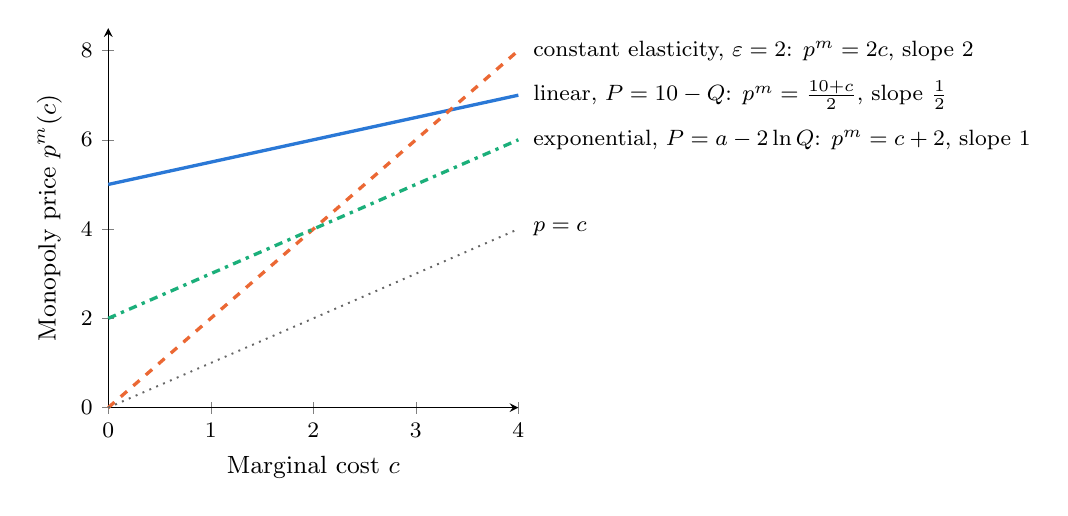
\begin{tikzpicture}
\definecolor{ptA}{HTML}{2A78D6}
\definecolor{ptB}{HTML}{EB6834}
\definecolor{ptC}{HTML}{1BAF7A}
\begin{axis}[
  width=0.56\textwidth, height=6.4cm,
  xmin=0, xmax=4, ymin=0, ymax=8.5,
  xlabel={Marginal cost $c$}, ylabel={Monopoly price $p^m(c)$},
  xtick={0,1,2,3,4}, ytick={0,2,4,6,8},
  tick label style={font=\footnotesize}, label style={font=\small},
  axis lines=left, clip=false, every axis plot/.append style={line width=1.2pt}]
  \addplot[domain=0:4, samples=2, color=ptA] {(10 + x)/2};
  \addplot[domain=0:4, samples=2, color=ptB, dashed] {2*x};
  \addplot[domain=0:4, samples=2, color=ptC, dash dot] {x + 2};
  \addplot[domain=0:4, samples=2, color=black!60, line width=0.7pt, dotted] {x};
  \node[anchor=west, font=\footnotesize, align=left] at (axis cs:4.05,8.0)
    {constant elasticity, $\varepsilon = 2$: $p^m = 2c$, slope $2$};
  \node[anchor=west, font=\footnotesize, align=left] at (axis cs:4.05,7.0)
    {linear, $P = 10 - Q$: $p^m = \frac{10 + c}{2}$, slope $\frac{1}{2}$};
  \node[anchor=west, font=\footnotesize, align=left] at (axis cs:4.05,6.0)
    {exponential, $P = a - 2\ln Q$: $p^m = c + 2$, slope $1$};
  \node[anchor=west, font=\footnotesize, align=left] at (axis cs:4.05,4.0)
    {$p = c$};
\end{axis}
\end{tikzpicture}
\caption{Monopoly price as a function of constant marginal cost for three demand curves. Linear demand
($a = 10$, $b = 1$) passes through one half of a cost change, exponential demand ($b = 2$) passes through all
of it, and constant-elasticity demand ($\varepsilon = 2$) passes through twice the change. The dotted line is
price equal to cost.}
\label{fig:02-pt-examples}
\end{figure}

\subsection{Conduct, curvature and rising marginal cost}\label{sec:02-pt-general}

We now allow imperfect competition of any degree and marginal cost that rises with output. The industry
satisfies the supply relation \eqref{eq:02-supply-relation} with conduct $\theta$, and a specific tax $t$ adds to
marginal cost. Write the supply relation with the \emph{marginal consumer surplus}
\begin{equation}\label{eq:02-ms}
ms(Q) = -QP'(Q) \ge 0 .
\end{equation}
The name comes from consumer surplus $CS(Q) = \int_0^Q P(x)\,\dd x - QP(Q)$, whose derivative is
$P - P - QP' = ms(Q)$. It is the gain in consumer surplus from one more unit of output. The supply relation then
reads $P(Q) - \theta\, ms(Q) = MC(Q) + t$: the markup equals conduct times the marginal consumer surplus. A
monopolist ($\theta = 1$) keeps its markup equal to the surplus it would hand to inframarginal consumers by
expanding.

\begin{assumption}[Pass-through under conduct]\label{ass:02-pt-general}
Inverse demand $P(Q)$ is twice continuously differentiable with $P' < 0$. Industry marginal cost $MC(Q)$ is
continuously differentiable with $MC' \ge 0$. Conduct $\theta \in [0, 1]$ does not vary with $t$. Equilibrium
output $Q(t)$ is positive, is continuous in $t$, and satisfies
\begin{equation}\label{eq:02-pt-supply}
P(Q) + \theta QP'(Q) = MC(Q) + t ,
\end{equation}
together with the stability condition
$\Lambda(Q) \equiv P'(Q) - \theta\, ms'(Q) - MC'(Q) < 0$.
\end{assumption}

As in \cref{ass:02-pt-monopoly}, the stability condition is the nonsingularity condition of the implicit function
theorem, and continuity keeps $Q(t)$ on one local branch of solutions. Hence $Q(t)$ is continuously differentiable.
The stability condition says that perceived marginal revenue $P - \theta\, ms$ cuts effective marginal cost from
above. It holds under monopoly by the second-order condition, and under symmetric Cournot competition by
\cref{ass:02-cournot} (see the proof of \cref{prop:02-pt-cournot}). Three elasticities summarize the primitives at the equilibrium. The demand elasticity is
$\varepsilon = -\frac{P}{QP'}$. The supply elasticity $\varepsilon_S = \frac{MC + t}{Q\, MC'}$ is the elasticity
of output with respect to effective marginal cost along the marginal-cost curve, and it is infinite when marginal
cost is flat. The term $\varepsilon_{ms} = \frac{ms}{Q\, ms'}$ is the elasticity of the inverse marginal-surplus
function, the reciprocal of the elasticity of $ms$ with respect to output \citep[p.~539]{WeylFabinger2013}.
Differentiating \eqref{eq:02-ms},
\begin{equation*}
ms'(Q) = -P'(Q) - QP''(Q) = -P'(Q)\Bigl(1 + \frac{QP''}{P'}\Bigr) = -P'(Q)\,(1 - \chi) ,
\end{equation*}
so $\frac{1}{\varepsilon_{ms}} = \frac{Q\,ms'}{ms} = \frac{-QP'(1 - \chi)}{-QP'} = 1 - \chi$. Exponential demand has
$\chi = 1$, a constant marginal consumer surplus, and $\frac{1}{\varepsilon_{ms}} = 0$.

\begin{proposition}[Pass-through under conduct, \citealp{WeylFabinger2013}]\label{prop:02-pt-general}
Under \cref{ass:02-pt-general},
\begin{equation}\label{eq:02-pt-general}
\rho = \frac{\dd P}{\dd t} = \frac{1}{1 + \frac{\varepsilon - \theta}{\varepsilon_S} + \frac{\theta}{\varepsilon_{ms}}}
= \frac{1}{1 + \theta(1 - \chi) + \frac{\varepsilon - \theta}{\varepsilon_S}} ,
\end{equation}
and the denominator is positive.
\end{proposition}

\begin{proof}
\emph{Step 1.} Differentiate $P(Q) - \theta\, ms(Q) = MC(Q) + t$ with respect to $t$:
\begin{equation*}
\bigl[P'(Q) - \theta\, ms'(Q)\bigr]\frac{\dd Q}{\dd t} = MC'(Q)\frac{\dd Q}{\dd t} + 1 .
\end{equation*}
Collecting terms gives $\Lambda\frac{\dd Q}{\dd t} = 1$, so $\frac{\dd Q}{\dd t} = \frac{1}{\Lambda} < 0$.

\emph{Step 2.} The price moves along the demand curve, so
\begin{equation*}
\rho = P'(Q)\frac{\dd Q}{\dd t} = \frac{P'}{P' - \theta\, ms' - MC'} = \frac{1}{1 - \theta\frac{ms'}{P'} - \frac{MC'}{P'}} .
\end{equation*}

\emph{Step 3.} The demand term is $-\frac{ms'}{P'} = 1 - \chi = \frac{1}{\varepsilon_{ms}}$ by the computation
above.

\emph{Step 4.} For the cost term, the definitions of the two elasticities give
$MC' = \frac{MC + t}{Q\varepsilon_S}$ and $\lvert P'\rvert = \frac{P}{\varepsilon Q}$. Hence
\begin{equation*}
-\frac{MC'}{P'} = \frac{MC'}{\lvert P'\rvert} = \frac{MC + t}{Q\varepsilon_S}\cdot\frac{\varepsilon Q}{P}
= \frac{\varepsilon}{\varepsilon_S}\cdot\frac{MC + t}{P} .
\end{equation*}

\emph{Step 5.} The Lerner form of \eqref{eq:02-pt-supply} is $\frac{P - MC - t}{P} = \frac{\theta}{\varepsilon}$,
as in \eqref{eq:02-theta-lerner}, so $\frac{MC + t}{P} = \frac{\varepsilon - \theta}{\varepsilon}$. Substituting into
Step 4 gives $-\frac{MC'}{P'} = \frac{\varepsilon - \theta}{\varepsilon_S}$.

\emph{Step 6.} Steps 2 to 5 give \eqref{eq:02-pt-general}. The denominator equals $\frac{\Lambda}{P'}$, a ratio
of two negative numbers, so it is positive.
\end{proof}

Step 2 has a geometric reading. With flat marginal cost, pass-through is the slope of inverse demand divided by
the slope of perceived marginal revenue, $\frac{P'}{P'(1 + \theta(1 - \chi))}$. A tax shifts the effective
marginal cost line up by $t$. Output falls until perceived marginal revenue has risen by $t$, and price rises by
the demand slope times the output change. When perceived marginal revenue is steep relative to demand, a small
output cut absorbs the tax and price rises little. Under exponential demand, marginal consumer surplus is constant, so
perceived marginal revenue is parallel to demand and price rises one for one. With rising marginal cost,
effective marginal cost also falls as output contracts. A smaller output cut then restores the supply relation,
and price rises less under every conduct.

\citet[eq.~(2), p.~548]{WeylFabinger2013} derive \eqref{eq:02-pt-general} for symmetric imperfect competition
and extend it to conduct that varies with output. Their denominator adds the term $\frac{\theta}{\varepsilon_\theta}
= Q\,\theta'(Q)$, where $\varepsilon_\theta = \frac{\theta}{Q\,\theta'(Q)}$ is the inverse of the elasticity of
conduct with respect to output. The version here assumes constant $\theta$, so this term vanishes.

\begin{corollary}[Special cases]\label{cor:02-pt-cases}
Under \cref{ass:02-pt-general}:
\begin{enumerate}[label=(\roman*)]
\item Price taking ($\theta = 0$) gives $\rho = \frac{\varepsilon_S}{\varepsilon_S + \varepsilon} \le 1$, with
  equality if and only if marginal cost is flat.
\item Flat marginal cost ($\varepsilon_S = \infty$) gives
  \begin{equation}\label{eq:02-pt-flat}
  \rho = \frac{1}{1 + \theta(1 - \chi)} .
  \end{equation}
\item Monopoly with flat marginal cost gives $\rho = \frac{1}{2 - \chi}$, which is \cref{prop:02-pt-monopoly}.
\item Symmetric Cournot competition among $N$ firms with flat marginal cost gives
  $\rho = \frac{N}{N + 1 - \chi}$. Linear demand gives $\frac{N}{N + 1}$, and constant elasticity gives
  $\frac{N\varepsilon}{N\varepsilon - 1} > 1$.
\item Monopoly with linear demand $P = a - bQ$ and linear marginal cost $MC = c_0 + kQ$ gives
  $\rho = \frac{b}{2b + k}$.
\end{enumerate}
\end{corollary}

\begin{proof}
(i) Setting $\theta = 0$ in \eqref{eq:02-pt-general} gives
$\rho = \frac{1}{1 + \frac{\varepsilon}{\varepsilon_S}} = \frac{\varepsilon_S}{\varepsilon_S + \varepsilon}$. The
same answer follows directly. A competitive industry with demand $Q(p)$ sets $p = MC(Q(p)) + t$.
Differentiating, $\rho = MC'(Q)\,Q'(p)\,\rho + 1$, so
\begin{equation*}
\rho = \frac{1}{1 + MC'\,\lvert Q'\rvert} = \frac{1}{1 + \frac{p}{Q\varepsilon_S}\cdot\frac{\varepsilon Q}{p}}
= \frac{\varepsilon_S}{\varepsilon_S + \varepsilon} ,
\end{equation*}
where the middle step uses $p = MC + t$. The ratio is below one whenever $\varepsilon_S < \infty$.

(ii) The term $\frac{\varepsilon - \theta}{\varepsilon_S}$ vanishes when $\varepsilon_S = \infty$.

(iii) Set $\theta = 1$ in \eqref{eq:02-pt-flat}. By \cref{lem:02-chi-direct} this equals
\eqref{eq:02-pt-logcurv}.

(iv) Each firm's first-order condition is $P + q_iP'(Q) = c + t$. Summing over the $N$ firms and dividing by
$N$ gives $P + \frac{1}{N}QP'(Q) = c + t$, the supply relation with $\theta = \frac{1}{N}$. Then
\eqref{eq:02-pt-flat} gives
\begin{equation*}
\rho = \frac{1}{1 + \frac{1 - \chi}{N}} = \frac{N}{N + 1 - \chi} .
\end{equation*}
Linear demand has $\chi = 0$. Constant elasticity has $\chi = 1 + \frac{1}{\varepsilon}$, so
$N + 1 - \chi = N - \frac{1}{\varepsilon}$ and $\rho = \frac{N\varepsilon}{N\varepsilon - 1}$. An interior
equilibrium requires $N\varepsilon > 1$.

(v) Here $\chi = 0$, and $\frac{\varepsilon - 1}{\varepsilon_S} = \frac{MC'}{\lvert P'\rvert} = \frac{k}{b}$ by
Steps 4 and 5 of the proof of \cref{prop:02-pt-general}. So $\rho = \frac{1}{2 + \frac{k}{b}} = \frac{b}{2b + k}$.
Directly, $a - 2bQ = c_0 + kQ + t$ gives $Q = \frac{a - c_0 - t}{2b + k}$ and $\frac{\dd P}{\dd t} = -b\frac{\dd Q}{\dd t} = \frac{b}{2b + k}$.
\end{proof}

Part (i) is the textbook incidence result for competitive markets. The side of the market with the smaller
elasticity bears more of the tax. Part (iv) shows that Cournot pass-through approaches one as $N$ grows, for any
fixed curvature. With constant elasticity it approaches one from above, so a more competitive industry passes
through less. \Cref{fig:02-pt-curvature} plots \eqref{eq:02-pt-flat} against curvature for four values of
conduct.

\begin{figure}[htbp]
\centering
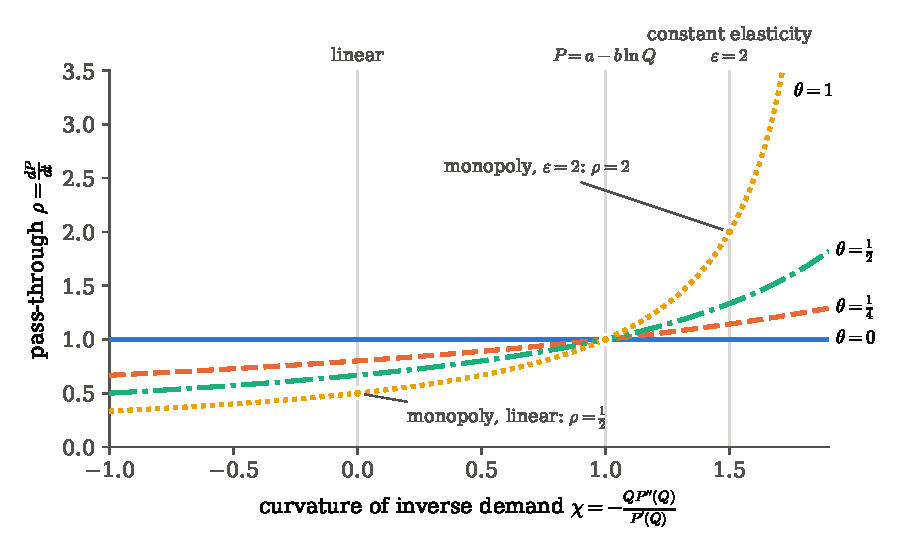
\includegraphics[width=0.86\textwidth]{figures/ch02/passthrough_curvature.pdf}
\caption{Pass-through with flat marginal cost, $\rho = \frac{1}{1 + \theta(1 - \chi)}$, against the curvature
of inverse demand for four values of conduct. All curves cross at $\chi = 1$ (exponential demand), where
$\rho = 1$ under every conduct. To the left of $\chi = 1$ market power lowers pass-through. To the right it
raises pass-through. The dots mark monopoly with linear demand ($\rho = \frac{1}{2}$), exponential demand
($\rho = 1$) and constant elasticity $\varepsilon = 2$ ($\rho = 2$). The monopoly curve is cut at
$\rho = 3.5$.}
\label{fig:02-pt-curvature}
\end{figure}

The figure shows the identification problem at a glance. Under competition with flat marginal cost, pass-through
is one for every demand curve. Market power rotates the line around the point $\chi = 1$. A pass-through above
one can come from strong market power with mild convexity or from weak market power with strong convexity.

\begin{corollary}[What pass-through reveals]\label{cor:02-pt-reveal}
Under \cref{ass:02-pt-general}:
\begin{enumerate}[label=(\roman*)]
\item Under price taking, $\rho \le 1$ for every demand curve and every nondecreasing marginal cost. A
  pass-through above one therefore rejects price taking.
\item With flat marginal cost, $\rho$ identifies only the product
  \begin{equation}\label{eq:02-pt-kappa}
  \theta(\chi - 1) = 1 - \frac{1}{\rho} .
  \end{equation}
  Every $\theta \in (0, 1]$ is consistent with every observed $\rho > 0$ for a suitable curvature. Price taking
  ($\theta = 0$) is consistent only with $\rho = 1$, whatever the curvature.
\item With rising marginal cost, $\theta(\chi - 1) = 1 - \frac{1}{\rho} + \frac{\varepsilon - \theta}{\varepsilon_S}
  \ge 1 - \frac{1}{\rho}$. Rising marginal cost lowers pass-through for given conduct and curvature, so it
  strengthens the rejection in (i). Price taking is then consistent with every $\rho \in (0, 1)$ for a suitable
  supply elasticity.
\item With constant-elasticity demand and flat marginal cost, $\theta = \varepsilon\bigl(1 - \frac{1}{\rho}\bigr)$.
  An estimate of the demand elasticity then converts pass-through into conduct.
\end{enumerate}
\end{corollary}

\begin{proof}
(i) is \cref{cor:02-pt-cases}(i). (ii) Rearrange \eqref{eq:02-pt-flat} as $\frac{1}{\rho} = 1 - \theta(\chi - 1)$.
The data enter only through $\rho$, so only the product $\theta(\chi - 1)$ is identified. Given $\rho$ and
$\theta > 0$, the curvature $\chi = 1 + \frac{1}{\theta}\bigl(1 - \frac{1}{\rho}\bigr)$ reproduces $\rho$. This
curvature satisfies the stability condition $1 + \theta(1 - \chi) = \frac{1}{\rho} > 0$, and under monopoly it
satisfies $\chi < 2$. A value $\rho \le 1$ requires $\chi \le 1$ when $\theta > 0$. With $\theta = 0$ the left
side of \eqref{eq:02-pt-kappa} is zero for every $\chi$, so $\rho = 1$. (iii) Rearrange \eqref{eq:02-pt-general}.
The added term is nonnegative because $\varepsilon \ge \theta$ whenever $P \ge MC + t$. With $\theta = 0$,
\cref{cor:02-pt-cases}(i) gives $\rho = \frac{\varepsilon_S}{\varepsilon_S + \varepsilon}$, which takes every
value in $(0, 1)$ as $\varepsilon_S$ ranges over $(0, \infty)$. (iv) Constant elasticity has $\chi - 1 = \frac{1}{\varepsilon}$.
Substitute into \eqref{eq:02-pt-kappa}.
\end{proof}

Part (i) is the robust content of a pass-through test. It needs no assumption on demand, and it needs only that
marginal cost does not fall with output. Two caveats apply. The price must be a product price, since a price
index can move for reasons of composition (\cref{sec:02-pt-composition}). The shifter must also move cost alone,
since a tax that shifts demand (for example through cross-border shopping) breaks the derivation. Part (ii) says
that a single market-wide cost shock moves the equilibrium along one demand curve, and that this movement cannot
separate conduct from curvature. \Cref{fig:02-pt-identified} draws the set of pairs $(\chi, \theta)$ consistent
with an illustrative pass-through of $1.07$. Separating the two requires an assumption on curvature, as in part
(iv), or variation that changes the slope of demand at a given price. \Cref{ch:conduct} develops both routes and
applies them to Sumner's cigarette data and to sugar refining.

\begin{figure}[htbp]
\centering
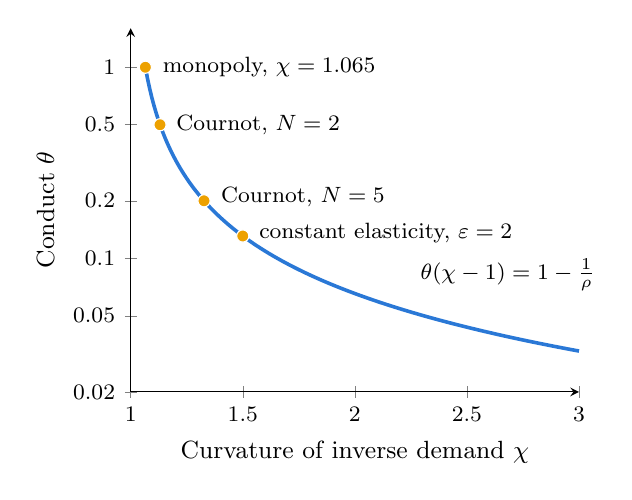
\begin{tikzpicture}
\definecolor{ptA}{HTML}{2A78D6}
\definecolor{ptD}{HTML}{EDA100}
\begin{axis}[
  width=0.6\textwidth, height=6.2cm,
  xmin=1, xmax=3, ymin=0.02, ymax=1.6, ymode=log,
  xlabel={Curvature of inverse demand $\chi$}, ylabel={Conduct $\theta$},
  xtick={1,1.5,2,2.5,3}, ytick={0.02,0.05,0.1,0.2,0.5,1},
  yticklabels={$0.02$,$0.05$,$0.1$,$0.2$,$0.5$,$1$},
  tick label style={font=\footnotesize}, label style={font=\small},
  axis lines=left, clip=false]
  \addplot[domain=1.0654:3, samples=200, color=ptA, line width=1.3pt] {0.0654206/(x - 1)};
  \addplot[only marks, mark=*, mark size=2.2pt, color=ptD, draw=white]
    coordinates {(1.0654,1) (1.1308,0.5) (1.3271,0.2) (1.5,0.13084)};
  \node[anchor=west, font=\footnotesize] at (axis cs:1.10,1.0) {monopoly, $\chi = 1.065$};
  \node[anchor=west, font=\footnotesize] at (axis cs:1.16,0.5) {Cournot, $N = 2$};
  \node[anchor=west, font=\footnotesize] at (axis cs:1.36,0.21) {Cournot, $N = 5$};
  \node[anchor=west, font=\footnotesize] at (axis cs:1.53,0.135) {constant elasticity, $\varepsilon = 2$};
  \node[anchor=south west, font=\footnotesize] at (axis cs:2.25,0.06) {$\theta(\chi - 1) = 1 - \frac{1}{\rho}$};
\end{axis}
\end{tikzpicture}
\caption{Pairs of demand curvature and conduct consistent with an illustrative pass-through $\rho = 1.07$ when
marginal cost is flat. Every point on the curve satisfies $\theta(\chi - 1) = 1 - \frac{1}{1.07} \approx 0.065$.
Symmetric Cournot with $N$ firms ($\theta = \frac{1}{N}$) fits with $\chi = 1 + 0.065N$. A constant-elasticity
demand with elasticity $\varepsilon$ has $\chi = 1 + \frac{1}{\varepsilon}$ and fits with
$\theta = 0.065\varepsilon$. The vertical axis is logarithmic.}
\label{fig:02-pt-identified}
\end{figure}

\subsection{Firm-specific versus industry-wide cost shocks in Cournot}\label{sec:02-pt-cournot}

So far a tax raised every firm's cost together. Many cost shocks hit one firm only: a local wage increase, a
plant outage, a merger's cost savings, or an exchange-rate shock to one importer. In a homogeneous-good market
all firms charge one price, and the question becomes how much that price responds to one firm's cost.

The linear Cournot model of \cref{ex:02-linear-cournot} gives the answer in closed form. With $P = a - bQ$ and
constant costs $c_1, \dots, c_N$,
\begin{equation*}
P^* = \frac{a + \sum_j c_j}{N + 1}, \qquad q_i^* = \frac{a - (N + 1)c_i + \sum_j c_j}{b(N + 1)} .
\end{equation*}
A rise in $c_i$ alone and a common rise $\dd c_j = \dd c$ for all $j$ give
\begin{equation*}
\frac{\dd P^*}{\dd c_i} = \frac{1}{N + 1}, \qquad \frac{\dd q_i^*}{\dd c_i} = -\frac{N}{b(N + 1)}, \qquad
\frac{\dd q_j^*}{\dd c_i} = \frac{1}{b(N + 1)} \;\; (j \ne i), \qquad \frac{\dd P^*}{\dd c} = \frac{N}{N + 1} .
\end{equation*}
Firm $i$'s margin $P^* - c_i$ falls by $\frac{N}{N + 1}$ per dollar of its own
cost increase, so the firm absorbs most of a firm-specific shock. The next result extends these formulas to
nonlinear demand.

\begin{proposition}[Cournot pass-through]\label{prop:02-pt-cournot}
Let (C1) and (C3) of \cref{ass:02-cournot} hold with constant marginal costs $c_1, \dots, c_N$, let all $N$ firms
be active, and suppose $P'(Q) + q_jP''(Q) < 0$ at the equilibrium for every $j$ (as (C2) guarantees).
Let $s_i = \frac{q_i}{Q}$ and let $\chi$ be the curvature \eqref{eq:02-chi} at the equilibrium output. Then
$N + 1 - \chi > 0$, and
\begin{equation}\label{eq:02-pt-cournot}
\frac{\dd P}{\dd c_i} = \frac{1}{N + 1 - \chi}, \qquad \frac{\dd P}{\dd c} = \frac{N}{N + 1 - \chi}, \qquad
\frac{\dd q_i}{\dd c_i} = \frac{N - (1 - s_i)\chi}{P'(Q)\,(N + 1 - \chi)} < 0 ,
\end{equation}
where $\frac{\dd P}{\dd c}$ is the response to a common shock.
\end{proposition}

\begin{proof}
We use the replacement functions of \cref{sec:02-cournot}. With constant costs, $\tilde q_i(Q)$ solves
$P(Q) + qP'(Q) = c_i$, so $\tilde q_i(Q) = \frac{c_i - P(Q)}{P'(Q)}$ near the equilibrium. Differentiating
$P(Q) + qP'(Q) = c_i$ in $c_i$ at fixed $Q$ gives $\frac{\partial\tilde q_i}{\partial c_i} = \frac{1}{P'}$.
Differentiating it in $Q$ gives $P' + \tilde q_i'P' + \tilde q_iP'' = 0$, so
\begin{equation*}
\tilde q_j'(Q) = -\Bigl(1 + \frac{q_jP''}{P'}\Bigr) = -\Bigl(1 + \frac{q_j}{Q}\cdot\frac{QP''}{P'}\Bigr)
= -(1 - s_j\chi) .
\end{equation*}
By assumption $P' + q_jP'' < 0$ at the equilibrium. Dividing by $P' < 0$ gives $1 - s_j\chi > 0$ for every $j$.
Summing over $j$ and using $\sum_j s_j = 1$,
\begin{equation*}
1 - \sum_j \tilde q_j'(Q) = 1 + \sum_j (1 - s_j\chi) = N + 1 - \chi > 0 .
\end{equation*}
Industry output solves $\sum_j \tilde q_j(Q) = Q$. Since the derivative of $\sum_j \tilde q_j(Q) - Q$ in $Q$ is
nonzero, the implicit function theorem applies. Differentiating in $c_i$, as in the proof of
\cref{prop:02-cournot-cs}, gives
\begin{equation*}
\frac{\dd Q}{\dd c_i} = \frac{\frac{\partial\tilde q_i}{\partial c_i}}{1 - \sum_j \tilde q_j'(Q)} .
\end{equation*}
Hence $\frac{\dd Q}{\dd c_i} = \frac{1}{P'(N + 1 - \chi)}$ and $\frac{\dd P}{\dd c_i} = P'\frac{\dd Q}{\dd c_i} = \frac{1}{N + 1 - \chi}$.
A common shock is the sum of $N$ firm-specific shocks, so $\frac{\dd P}{\dd c} = \sum_i\frac{\dd P}{\dd c_i} = \frac{N}{N + 1 - \chi}$.
For firm $i$'s own output, $q_i = \tilde q_i(Q)$ in equilibrium, so
\begin{equation*}
\frac{\dd q_i}{\dd c_i} = \frac{\partial\tilde q_i}{\partial c_i} + \tilde q_i'(Q)\frac{\dd Q}{\dd c_i}
= \frac{1}{P'}\Bigl[1 - \frac{1 - s_i\chi}{N + 1 - \chi}\Bigr]
= \frac{N - (1 - s_i)\chi}{P'(N + 1 - \chi)} .
\end{equation*}
The numerator equals $1 + \sum_{j \ne i}(1 - s_j\chi) > 0$, and $P' < 0$, so $\frac{\dd q_i}{\dd c_i} < 0$.
\end{proof}

Three features of \eqref{eq:02-pt-cournot} stand out. First, the price response to a firm-specific shock does
not depend on the firm's share. A large firm and a small firm move the price by the same amount after equal
cost increases. The direct effect on a firm's replacement output, $\frac{1}{P'}$, does not depend on its size, and
rivals respond only to total output. Second, the
common-shock pass-through equals \cref{cor:02-pt-cases}(iv) even with asymmetric costs. Third, the ratio of the
two is $N$ for any demand curve. A firm-specific shock moves the market price by only a fraction
$\frac{1}{N + 1 - \chi}$ of the shock, and the firm bears the rest through a lower margin.

The distinction matters for empirical work. A market-wide shifter, such as an excise tax, moves the industry
along the market demand curve. Its pass-through speaks to industry conduct and market demand curvature, as in
\cref{sec:02-pt-general}. A firm-specific shifter, such as a firm's own input price, moves the equilibrium along
the firm's residual demand curve, which includes rivals' supply responses. \citet{BakerBresnahan1988} use such
shifters to estimate residual demand directly (\cref{ch:conduct}). The distinction also matters for mergers.
The cost savings of a merger are specific to the merged firm, so the relevant pass-through is the
firm-specific one. Using an industry-wide rate would overstate how much of the savings reaches consumers
(\cref{ch:mergers}).

\subsection{Incidence}\label{sec:02-pt-incidence}

Pass-through determines who bears a tax. Consumer surplus is $CS = \int_0^Q P(x)\,\dd x - P(Q)Q$. Producer surplus
is variable profit, $PS = P(Q)Q - C(Q) - tQ$, where $C$ is industry variable cost with $C' = MC$ (as with
symmetric firms). Tax revenue is $R = tQ$.

\begin{proposition}[Incidence under conduct, {\citealp[pp.~546--548]{WeylFabinger2013}}]\label{prop:02-incidence}
Under \cref{ass:02-pt-general}, a small change in the specific tax changes surplus by
\begin{equation*}
\frac{\dd CS}{\dd t} = -\rho Q, \qquad \frac{\dd PS}{\dd t} = -\bigl[1 - (1 - \theta)\rho\bigr]Q .
\end{equation*}
When the producer burden is nonzero, the \emph{incidence ratio}, consumer burden divided by producer burden, is
\begin{equation}\label{eq:02-incidence}
I = \frac{\frac{\dd CS}{\dd t}}{\frac{\dd PS}{\dd t}} = \frac{\rho}{1 - (1 - \theta)\rho} .
\end{equation}
Total surplus $W = CS + PS + R$ satisfies $\frac{\dd W}{\dd t} = -\theta\rho Q + t\frac{\dd Q}{\dd t}$.
\end{proposition}

\begin{proof}
\emph{Consumers.} By Leibniz's rule,
\begin{equation*}
\frac{\dd CS}{\dd t} = P(Q)\frac{\dd Q}{\dd t} - \Bigl[P'(Q)Q + P(Q)\Bigr]\frac{\dd Q}{\dd t} = -QP'(Q)\frac{\dd Q}{\dd t} = -Q\rho ,
\end{equation*}
since $\rho = P'\frac{\dd Q}{\dd t}$.

\emph{Producers.} Differentiating $PS$,
\begin{equation*}
\frac{\dd PS}{\dd t} = P'Q\frac{\dd Q}{\dd t} + P\frac{\dd Q}{\dd t} - MC\frac{\dd Q}{\dd t} - Q - t\frac{\dd Q}{\dd t}
= Q(\rho - 1) + (P - MC - t)\frac{\dd Q}{\dd t} .
\end{equation*}
The supply relation \eqref{eq:02-pt-supply} gives $P - MC - t = -\theta QP'$, and $\frac{\dd Q}{\dd t} = \frac{\rho}{P'}$.
Hence $(P - MC - t)\frac{\dd Q}{\dd t} = -\theta QP'\cdot\frac{\rho}{P'} = -\theta\rho Q$, and
\begin{equation*}
\frac{\dd PS}{\dd t} = Q(\rho - 1) - \theta\rho Q = -Q\bigl[1 - (1 - \theta)\rho\bigr] .
\end{equation*}
Dividing the two derivatives gives \eqref{eq:02-incidence}.

\emph{Total surplus.} Revenue changes by $\frac{\dd R}{\dd t} = Q + t\frac{\dd Q}{\dd t}$. Adding the three derivatives,
\begin{equation*}
\frac{\dd W}{\dd t} = -\rho Q - Q + (1 - \theta)\rho Q + Q + t\frac{\dd Q}{\dd t} = -\theta\rho Q + t\frac{\dd Q}{\dd t} .
\qedhere
\end{equation*}
\end{proof}

\citet[p.~546]{WeylFabinger2013} credit \citet{AtkinDonaldson2012} with first deriving the formula for
$\frac{\dd PS}{\dd t}$, which extends the monopoly case to general conduct.

The special cases are instructive. Under price taking, $I = \frac{\rho}{1 - \rho}$. With
$\rho = \frac{\varepsilon_S}{\varepsilon_S + \varepsilon}$ from \cref{cor:02-pt-cases}(i), this is
$I = \frac{\varepsilon_S}{\varepsilon}$, the classic rule that the burden falls on the less elastic side. With flat
marginal cost, competitive producers bear nothing. Under monopoly, $\frac{\dd PS}{\dd t} = -Q$ whatever the demand
curve, which is the envelope theorem at work (\cref{app:math}), and $I = \rho$. Consumers bear more than the
monopolist exactly when $\rho > 1$. With linear demand, flat cost and conduct $\theta$, $\rho = \frac{1}{1 + \theta}$
and
\begin{equation*}
I = \frac{\frac{1}{1 + \theta}}{1 - \frac{1 - \theta}{1 + \theta}} = \frac{\frac{1}{1 + \theta}}{\frac{2\theta}{1 + \theta}}
= \frac{1}{2\theta} .
\end{equation*}
A linear monopoly ($\theta = 1$) puts one third of the private burden on consumers, and a symmetric Cournot duopoly
($\theta = \frac{1}{2}$) splits it equally.

Market power changes incidence in two ways that competitive analysis misses. First, consumers can bear more than
the full tax ($\rho > 1$) while producers still lose. With constant elasticity $\varepsilon = 2$, a monopolist
passes through $\rho = 2$, consumers lose $2Q$ per unit of tax and the monopolist loses $Q$. Second, producers
can gain from a tax. The producer burden is negative when $\rho > \frac{1}{1 - \theta}$. With flat marginal cost
this condition reduces to $\theta(2 - \chi) < 0$, that is $\chi > 2$ for $\theta > 0$. Monopoly rules this out
through its second-order condition, but oligopoly with $\theta < 1$ allows $2 < \chi < 1 + \frac{1}{\theta}$.
In symmetric Cournot with constant elasticity,
\begin{equation*}
1 - \Bigl(1 - \frac{1}{N}\Bigr)\frac{N\varepsilon}{N\varepsilon - 1} = \frac{\varepsilon - 1}{N\varepsilon - 1} ,
\end{equation*}
which is negative when $\frac{1}{N} < \varepsilon < 1$. A common cost increase then raises industry profit. It
pushes output toward the level that maximizes joint profit, which the firms could not reach on their own.

The total-surplus formula adds a third difference. Under competition the first tax dollar has no deadweight cost,
because $\frac{\dd W}{\dd t} = 0$ at $t = 0$ when $\theta = 0$. Under market power the first dollar already costs
$\theta\rho Q$, because output starts below its efficient level (\cref{sec:02-welfare}). Linear monopoly loses
$\frac{Q}{2}$ of surplus per unit of tax at $t = 0$, half of the revenue raised. \citet[pp.~537 and
546]{WeylFabinger2013} state that this excess burden is $\rho$ per unit of revenue under monopoly and positive
whenever $\theta > 0$. We add the total-surplus formula itself, which also holds at $t > 0$.

\begin{remark}[Ad valorem taxes]\label{rem:02-pt-adval}
An \emph{ad valorem tax} at rate $t_a$ takes a fraction $t_a$ of the price. Firms receive $(1 - t_a)P$, and the
supply relation becomes $(1 - t_a)(P + \theta QP') = MC(Q)$, that is $P + \theta QP' = \frac{MC(Q)}{1 - t_a}$.
An ad valorem tax therefore scales effective marginal cost by $\frac{1}{1 - t_a}$. At $t_a = 0$ a small rate
$\dd t_a$ raises effective marginal cost by $MC\,\dd t_a$, so $\frac{\dd P}{\dd t_a} = \rho\, MC$. A specific tax
$\dd t = P\,\dd t_a$ raises the same revenue to first order and raises price by $\rho P\,\dd t_a$. At $t_a = 0$
the Lerner form gives $MC = (1 - \frac{\theta}{\varepsilon})P$, so the ad valorem tax raises price less per dollar
of revenue whenever $\theta > 0$. Under competition the two taxes coincide to first order. The incidence formulas for ad valorem taxes
are left to \cref{sec:02-exercises}.
\end{remark}

\subsection{Measured prices and composition}\label{sec:02-pt-composition}

Pass-through regressions often use a price index, an average across products, as the dependent variable. The
index can move even when no product's price moves, because the mix of products bought changes.

\begin{remark}[Composition bias]\label{rem:02-pt-composition}
Let the observed price be the quantity-weighted average $\bar p = \sum_j w_jp_j$, with weights $w_j \ge 0$
summing to one. Differentiating with respect to the tax,
\begin{equation}\label{eq:02-pt-composition}
\frac{\dd \bar p}{\dd t} = \underbrace{\sum_j w_j\frac{\dd p_j}{\dd t}}_{\text{price effect}}
+ \underbrace{\sum_j p_j\frac{\dd w_j}{\dd t}}_{\text{composition effect}} .
\end{equation}
The first term is the average of product-level pass-through. The second term is nonzero whenever the tax changes
the mix of purchases. A regression of $\bar p$ on $t$ estimates the sum.
\end{remark}

A specific tax tends to make the composition effect positive. It raises every price by a similar dollar amount,
which is a larger percentage of a cheap product's price. Suppose a cheap and an expensive product have prices
$p_L < p_H$, and each price rises one for one with the tax. The relative price $\frac{p_H + t}{p_L + t}$ has
derivative $\frac{p_L - p_H}{(p_L + t)^2} < 0$ in $t$, so the expensive product becomes relatively cheaper. If
buyers respond to relative prices, the weight $w_H$ rises, and the composition effect
$(p_H - p_L)\frac{\dd w_H}{\dd t}$ is positive. A numerical illustration makes the size concrete. Let $p_L = 1$,
$p_H = 2$ and $w_H = 0.5$, and let a tax of $0.10$ raise both prices by $0.10$ and $w_H$ to $0.52$. The index
rises from $1.50$ to $0.48 \times 1.10 + 0.52 \times 2.10 = 1.62$, so the measured pass-through is $1.2$ although
each product's pass-through is exactly one.

The bias pushes a test toward rejecting price taking, because it can create $\hat\rho > 1$ from product-level
pass-through equal to one. The remedies are to estimate pass-through at the product level, or to use a
fixed-weight index $\sum_j w_j^0 p_j$ that holds the weights at their pre-tax values. The same logic runs in the
opposite direction when demand peaks. \citet{NevoHatzitaskos2005} study canned tuna, whose average price falls
during Lent although demand is high. They argue that a shift of purchases toward cheaper products explains much
of the fall in the average price paid. In their supermarket data, the Lent coefficient is $-1.78$ cents per ounce
for the quantity-weighted tuna price index and $-0.51$ for a fixed-weight index \citep[p.~13 and
Table~3]{NevoHatzitaskos2005}.
\Cref{ch:conduct} returns to composition as one of the three standard critiques of Sumner's cigarette-tax test.

Pass-through thus carries information about market power, but only jointly with the curvature of demand and the
slope of marginal cost. Pass-through above one is hard to reconcile with price taking. Beyond that, a pass-through
estimate must be combined with an assumption or a second source of variation before it reveals conduct. The
incidence of taxes, the consumer benefits of cost savings and the price effects of mergers all inherit this
dependence on curvature.

\section{Welfare and the deadweight loss of market power}\label{sec:02-welfare}

The previous sections asked how far price exceeds marginal cost and why. This section asks what the gap costs
society. A positive correlation between concentration and margins, or an estimated conduct parameter above zero,
does not by itself tell us that the losses are large. To answer the normative question we need a measure of welfare,
a way to compute it from demand and cost, and a sense of its likely size. We first set up the standard
partial-equilibrium apparatus and derive closed forms for linear demand. We then present the Harberger
approximation and the debate it started. The section closes with three qualifications: production inefficiency
across firms, entry, and the trade-off between market power and cost savings in mergers.

\subsection{Surplus measures}\label{sec:02-surplus}

We work in a single market and use partial-equilibrium welfare analysis.

\begin{assumption}[Partial-equilibrium welfare]\label{ass:02-welfare}
\leavevmode
\begin{enumerate}[label=(W\arabic*)]
\item Consumers have quasi-linear utility in the good and a numeraire, so market demand has no income effects.
      The area under the inverse demand curve then measures willingness to pay in units of the numeraire.
\item The industry produces output $Q$ at the minimum total variable cost $C(Q)$, with $C$ increasing and
      convex. Fixed costs are set aside until \cref{sec:02-second-best}.
\item A dollar of consumer surplus and a dollar of profit carry equal social weight.
\end{enumerate}
\end{assumption}

Assumption (W1) makes the Marshallian consumer surplus an exact money measure of welfare. Without it, the
compensating and equivalent variations of \cref{ch:aids} replace the area under the demand curve. Assumption (W3)
is the \emph{total-surplus standard}. Antitrust practice often uses a \emph{consumer-surplus standard} instead,
which counts only the first term. The distinction matters most for mergers (\cref{ch:mergers}).

\begin{definition}[Surplus and deadweight loss]\label{def:02-surplus}
At industry output $Q$ and price $P(Q)$, \emph{consumer surplus}, \emph{producer surplus} and \emph{total surplus}
are
\begin{align}
CS(Q) &= \int_0^{Q} P(x)\,\dd x - P(Q)\,Q, \label{eq:02-cs}\\
PS(Q) &= P(Q)\,Q - C(Q), \label{eq:02-ps}\\
W(Q)  &= CS(Q) + PS(Q) = \int_0^{Q} P(x)\,\dd x - C(Q). \label{eq:02-total-surplus}
\end{align}
Let $Q^c$ maximize $W$. The \emph{deadweight loss} at output $Q$ is $\mathit{DWL}(Q) = W(Q^c) - W(Q)$.
\end{definition}

The price drops out of total surplus because payments from consumers to producers are transfers. Differentiating
\eqref{eq:02-total-surplus} with respect to $Q$ gives
\begin{equation*}
W'(Q) = P(Q) - C'(Q), \qquad W''(Q) = P'(Q) - C''(Q) < 0 .
\end{equation*}
Total surplus is therefore strictly concave, and it is maximized at the output where $P(Q^c) = C'(Q^c)$. This is
the price-taking output, so the first-best benchmark is the competitive outcome. For any $Q < Q^c$, the fundamental
theorem of calculus gives
\begin{equation}\label{eq:02-dwl-general}
\mathit{DWL}(Q) = W(Q^c) - W(Q) = \int_{Q}^{Q^c} \bigl[P(x) - C'(x)\bigr]\,\dd x .
\end{equation}
The integrand is the gap between willingness to pay and marginal cost on each unit that market power removes. With
constant marginal cost $c$, the deadweight loss is the area between the demand curve and the horizontal line at
$c$, from $Q$ to $Q^c$. Producer surplus is then variable profit, $PS = (P - c)\,Q$.

\begin{example}[The monopoly benchmark]\label{ex:02-welfare-monopoly}
Take the market of \cref{fig:02-monopoly}: $P(Q) = 10 - Q$ and $c = 2$. The competitive output solves
$10 - Q = 2$, so $Q^c = 8$ and maximal surplus is $W(Q^c) = \frac{1}{2}\cdot 8 \cdot 8 = 32$. The monopolist sells
$Q^m = 4$ at $p^m = 6$. Consumer surplus is $\frac{1}{2}\cdot 4 \cdot 4 = 8$, profit is $(6 - 2)\cdot 4 = 16$, and
the deadweight loss is $\frac{1}{2}(6 - 2)(8 - 4) = 8$. Consumers keep one quarter of the potential surplus, the
monopolist takes one half, and one quarter is destroyed.
\end{example}

\begin{remark}[An output subsidy restores efficiency]\label{rem:02-subsidy}
A per-unit subsidy can remove the monopoly distortion \citep[sec.~1.1.1.3]{Tirole1988}. Let consumers pay $p + t$
for each unit on which the firm receives $p$, so that $t < 0$ is a subsidy. The firm chooses $p$ to maximize
$pQ(p + t) - C\bigl(Q(p + t)\bigr)$, and its first-order condition is
\[
  Q(p + t) + Q'(p + t)\bigl[p - C'(Q)\bigr] = 0 .
\]
Write $p_b = p + t$ for the consumer price and substitute $p = p_b - t$:
\[
  \bigl[Q(p_b) - t\,Q'(p_b)\bigr] + Q'(p_b)\bigl[p_b - C'(Q)\bigr] = 0 .
\]
Efficiency requires the consumer price to equal marginal cost at the competitive price $p^c$. The second bracket
then vanishes, so the first must vanish too:
\[
  t = \frac{Q(p^c)}{Q'(p^c)} < 0, \qquad \frac{t}{p^c} = -\frac{1}{\varepsilon(p^c)} .
\]
The subsidy per unit, as a fraction of the competitive price, is the inverse elasticity of demand at that price. In
\cref{ex:02-welfare-monopoly}, $p^c = 2$, $Q(p^c) = 8$ and $Q' = -1$, so $t = -8$. The firm receives 10 per unit,
consumers pay 2 and buy the efficient 8 units, and total surplus reaches its maximum of 32. The firm's profit of 64
equals the subsidy bill of 64.

The subsidy has few advocates, and Tirole lists the objections. The total-surplus standard gives a dollar of profit
the same weight as a dollar of consumer surplus, so it records no cost for the transfer to shareholders. The
government must know the elasticity of demand and the firm's marginal cost. The firm gains from overstating the
subsidy it needs, and it is reluctant to reveal its costs. Schemes that reward the firm for low prices lead into the
theory of regulation, which this chapter does not pursue.
\end{remark}

\subsection{Linear demand with conduct}\label{sec:02-dwl-linear}

The conduct parameter of \cref{sec:02-conduct} indexes market power continuously, from price taking ($\theta = 0$)
through symmetric Cournot ($\theta = \frac{1}{N}$) to monopoly ($\theta = 1$). With linear demand, every welfare
quantity has a closed form in $\theta$.

\begin{proposition}[Welfare with linear demand and conduct $\theta$]\label{prop:02-dwl-linear}
Let $P(Q) = a - bQ$ with $a > c \ge 0$ and $b > 0$, let marginal cost be constant at $c$, and let price satisfy the
supply relation \eqref{eq:02-supply-relation} with conduct $\theta \in [0, 1]$. Then
\begin{enumerate}[label=(\roman*)]
\item Equilibrium output and markup are $Q(\theta) = \frac{a - c}{b(1 + \theta)}$ and
      $P(\theta) - c = \frac{\theta (a - c)}{1 + \theta}$.
\item Maximal total surplus is $W^{\max} = \frac{(a - c)^2}{2b}$.
\item Consumer surplus, profit and deadweight loss are the shares $\frac{1}{(1 + \theta)^2}$,
      $\frac{2\theta}{(1 + \theta)^2}$ and $\frac{\theta^2}{(1 + \theta)^2}$ of $W^{\max}$. In particular
      \begin{equation}\label{eq:02-dwl-linear}
      \mathit{DWL}(\theta) = \frac{\theta^2 (a - c)^2}{2b(1 + \theta)^2}.
      \end{equation}
\end{enumerate}
\end{proposition}

\begin{proof}
(i) This repeats part (i) of \cref{ex:02-pt-examples}. The supply relation is $P = c - \theta Q P'(Q)$, and here
$P'(Q) = -b$. Substituting the demand curve,
\begin{align*}
a - bQ &= c + \theta b Q, \\
a - c &= b(1 + \theta)\, Q, \\
Q(\theta) &= \frac{a - c}{b(1 + \theta)} .
\end{align*}
The markup is $P - c = \theta b Q = \frac{\theta(a - c)}{1 + \theta}$.

(ii) The competitive output solves $a - bQ = c$, so $Q^c = \frac{a - c}{b}$. Then
\begin{equation*}
W^{\max} = \int_0^{Q^c} (a - bx - c)\,\dd x = (a - c)\,Q^c - \frac{b}{2}(Q^c)^2
= \frac{(a - c)^2}{b} - \frac{(a - c)^2}{2b} = \frac{(a - c)^2}{2b} .
\end{equation*}

(iii) Consumer surplus is the triangle above the price,
\begin{equation*}
CS = \int_0^{Q}(a - bx)\,\dd x - (a - bQ)\,Q = aQ - \frac{b}{2}Q^2 - aQ + bQ^2 = \frac{b}{2}Q^2
= \frac{(a - c)^2}{2b(1 + \theta)^2} .
\end{equation*}
Profit is the rectangle
\begin{equation*}
\pi = (P - c)\,Q = \frac{\theta(a - c)}{1 + \theta}\cdot\frac{a - c}{b(1 + \theta)} = \frac{\theta(a - c)^2}{b(1 + \theta)^2} .
\end{equation*}
The deadweight loss is the triangle with height $P - c$ and base
$Q^c - Q = \frac{a - c}{b}\left(1 - \frac{1}{1 + \theta}\right) = \frac{\theta(a - c)}{b(1 + \theta)}$, so
\begin{equation*}
\mathit{DWL} = \frac{1}{2}\cdot\frac{\theta(a - c)}{1 + \theta}\cdot\frac{\theta(a - c)}{b(1 + \theta)}
= \frac{\theta^2(a - c)^2}{2b(1 + \theta)^2} .
\end{equation*}
Dividing each expression by $W^{\max}$ gives the three shares. As a check, the three shares sum to
\[
\frac{1 + 2\theta + \theta^2}{(1 + \theta)^2} = 1 . \qedhere
\]
\end{proof}

\begin{corollary}[Monopoly and Cournot]\label{cor:02-dwl-cournot}
Under monopoly ($\theta = 1$) the shares are $\frac{1}{4}$, $\frac{1}{2}$ and $\frac{1}{4}$. Under symmetric Cournot
with $N$ firms ($\theta = \frac{1}{N}$), multiplying numerator and denominator by $N^2$ gives
\begin{equation}\label{eq:02-dwl-cournot}
\frac{CS}{W^{\max}} = \frac{N^2}{(N + 1)^2}, \qquad
\frac{\pi}{W^{\max}} = \frac{2N}{(N + 1)^2}, \qquad
\frac{\mathit{DWL}}{W^{\max}} = \frac{1}{(N + 1)^2}.
\end{equation}
For every $\theta > 0$ the ratio of deadweight loss to profit is $\frac{\mathit{DWL}}{\pi} = \frac{\theta}{2}$.
\end{corollary}

\begin{table}[htbp]
\centering
\begin{threeparttable}
\caption{Division of the maximal surplus under linear demand}
\label{tab:02-welfare-shares}
\small
\renewcommand{\arraystretch}{1.6}
\begin{tabular}{@{}lccccc@{}}
\toprule
Market & $\theta$ & Consumer surplus & Profit & Deadweight loss & $\frac{\mathit{DWL}}{\pi}$ \\
\midrule
Price taking      & $0$           & $1$                & $0$               & $0$              & n.a. \\
Cournot, $N = 5$  & $\frac{1}{5}$ & $\frac{25}{36}$    & $\frac{10}{36}$   & $\frac{1}{36}$   & $0.10$ \\
Cournot, $N = 4$  & $\frac{1}{4}$ & $\frac{16}{25}$    & $\frac{8}{25}$    & $\frac{1}{25}$   & $0.125$ \\
Cournot, $N = 3$  & $\frac{1}{3}$ & $\frac{9}{16}$     & $\frac{6}{16}$    & $\frac{1}{16}$   & $0.17$ \\
Cournot, $N = 2$  & $\frac{1}{2}$ & $\frac{4}{9}$      & $\frac{4}{9}$     & $\frac{1}{9}$    & $0.25$ \\
Monopoly          & $1$           & $\frac{1}{4}$      & $\frac{1}{2}$     & $\frac{1}{4}$    & $0.50$ \\
\bottomrule
\end{tabular}
\begin{tablenotes}\footnotesize
\item Notes: Shares of $W^{\max} = \frac{(a - c)^2}{2b}$ from \cref{prop:02-dwl-linear} and
\cref{cor:02-dwl-cournot}. The last column is $\frac{\theta}{2}$.
\end{tablenotes}
\end{threeparttable}
\end{table}

\Cref{tab:02-welfare-shares} carries two lessons. First, near competition the transfer to producers is first order
in $\theta$, while the deadweight loss is second order. For small $\theta$ the profit share is close to $2\theta$ and
the loss share is close to $\theta^2$. Second, the deadweight loss falls quickly with the number of Cournot firms.
It is $\frac{1}{9}$, or 11.1 percent of maximal surplus, under duopoly and $\frac{1}{36}$, or 2.8 percent, with five
firms. With five firms the transfer to producers is ten times the deadweight loss. With linear demand, concern about
market power in moderately concentrated markets is therefore largely a concern about distribution, unless market power also
raises costs or wastes resources. The rest of this section examines those two channels.

\subsection{The Harberger approximation}\label{sec:02-harberger}

Closed forms need a demand curve. To estimate losses across many industries with little information,
\citet{Harberger1954} used a local approximation that needs only revenue, the Lerner index and the elasticity of
demand. We derive it in general and then turn to its uses.

Fix an equilibrium with output $Q$, price $P = P(Q)$ and constant marginal cost $c < P$. Approximate inverse demand
between $Q$ and $Q^c$ by its tangent at $Q$:
\begin{equation*}
P(x) \approx P(Q) + P'(Q)(x - Q).
\end{equation*}
The competitive output then solves $P(Q) + P'(Q)(Q^c - Q) = c$, so
\begin{equation*}
Q^c - Q \approx \frac{P(Q) - c}{-P'(Q)} .
\end{equation*}
Substituting the tangent into \eqref{eq:02-dwl-general} and integrating,
\begin{align*}
\mathit{DWL} &\approx \int_Q^{Q^c}\bigl[P(Q) - c + P'(Q)(x - Q)\bigr]\,\dd x \\
&= (P - c)(Q^c - Q) + \frac{1}{2}P'(Q)(Q^c - Q)^2 \\
&= \frac{(P - c)^2}{-P'(Q)} - \frac{1}{2}\cdot\frac{(P - c)^2}{-P'(Q)}
 = \frac{1}{2}\cdot\frac{(P - c)^2}{-P'(Q)} .
\end{align*}
The market elasticity is $\varepsilon = -\frac{1}{P'(Q)}\frac{P}{Q}$, so $-P'(Q) = \frac{P}{\varepsilon Q}$. With the
Lerner index $L = \frac{P - c}{P}$ and revenue $R = PQ$, this gives the \emph{Harberger approximation}
\begin{equation}\label{eq:02-harberger}
\mathit{DWL} \approx \frac{1}{2}\,(P - c)\,(Q^c - Q) \approx \frac{1}{2}\,\varepsilon\, L^2\, R .
\end{equation}
The loss is half the markup times the lost output, and the lost output is approximately $\varepsilon L Q$. The loss
is proportional to the square of the Lerner index, which is why small markups imply very small losses.

The approximation takes a simple form under any conduct. The supply relation in Lerner form,
\eqref{eq:02-theta-lerner}, gives $L = \frac{\theta}{\varepsilon}$. Substituting into \eqref{eq:02-harberger} and
using profit $\pi = (P - c)Q = LR$,
\begin{equation}\label{eq:02-harberger-theta}
\mathit{DWL} \approx \frac{\theta^2}{2\varepsilon}\,R = \frac{\theta}{2}\,L R = \frac{\theta}{2}\,\pi .
\end{equation}
Under monopoly, $\theta = 1$ and $L = \frac{1}{\varepsilon}$, so $\mathit{DWL} \approx \frac{R}{2\varepsilon} =
\frac{1}{2}LR$: the triangle is about half the profit rectangle. For linear demand the tangent is the demand curve,
so \eqref{eq:02-harberger} and \eqref{eq:02-harberger-theta} hold exactly. They reproduce
\cref{prop:02-dwl-linear} and the ratio $\frac{\mathit{DWL}}{\pi} = \frac{\theta}{2}$ of \cref{cor:02-dwl-cournot}.

\begin{remark}[Accuracy with convex demand]\label{rem:02-harberger-accuracy}
The tangent understates the area under a convex demand curve, so \eqref{eq:02-harberger} understates large losses.
Take constant-elasticity demand $Q(p) = Ap^{-\varepsilon}$ with $\varepsilon > 1$, marginal cost $c > 0$ and
monopoly pricing, $p^m = \frac{\varepsilon}{\varepsilon - 1}c$. The exact loss is the consumer surplus lost minus the profit gained,
\begin{equation*}
\mathit{DWL} = \int_c^{p^m} Ap^{-\varepsilon}\,\dd p - (p^m - c)A(p^m)^{-\varepsilon} .
\end{equation*}
Integrating, dividing by revenue $R = A(p^m)^{1-\varepsilon}$ and using $\frac{c}{p^m} = \frac{\varepsilon - 1}{\varepsilon}$,
\begin{equation*}
\frac{\mathit{DWL}}{R} = \frac{1}{\varepsilon - 1}\left[\left(\frac{\varepsilon - 1}{\varepsilon}\right)^{1 - \varepsilon} - 1\right]
- \frac{1}{\varepsilon} .
\end{equation*}
The Harberger approximation gives $\frac{1}{2\varepsilon}$. For $\varepsilon = 2$ the exact loss is $\frac{1}{2}R$,
twice the approximation of $\frac{1}{4}R$, and as large as the monopoly profit itself. Our computations give exact
to approximate ratios of 2.39, 2.00, 1.75 and 1.60 for $\varepsilon = 1.5, 2, 3$ and $5$. The approximation
improves as the markup falls, as it should for a second-order expansion.
\end{remark}

\begin{remark}[The deadweight loss need not fall with the elasticity]\label{rem:02-dwl-elasticity}
The Lerner index $\frac{1}{\varepsilon}$ falls as demand becomes more elastic, but the deadweight loss need not
\citep[sec.~1.1.1.2]{Tirole1988}. Where demand is inelastic, a high price moves little output and mostly transfers
money from consumers to the firm. Take $Q(p) = p^{-\varepsilon}$ with $\varepsilon > 1$ and constant marginal cost
$c > 0$ \citep[Exercise~1.1]{Tirole1988}. Maximal surplus is the consumer surplus at price $c$,
\[
  W^c = \int_c^{\infty} p^{-\varepsilon}\,\dd p = \frac{c^{1 - \varepsilon}}{\varepsilon - 1} .
\]
At $p^m = \frac{\varepsilon}{\varepsilon - 1}c$, consumer surplus is $\frac{(p^m)^{1 - \varepsilon}}{\varepsilon - 1}$
and profit is $(p^m - c)(p^m)^{-\varepsilon} = \frac{(p^m)^{1 - \varepsilon}}{\varepsilon}$, since $p^m - c =
\frac{p^m}{\varepsilon}$. Let $\kappa = \left(\frac{p^m}{c}\right)^{1 - \varepsilon} = \left(\frac{\varepsilon -
1}{\varepsilon}\right)^{\varepsilon - 1}$, a symbol local to this remark. Dividing by $W^c$,
\[
  \frac{CS^m}{W^c} = \kappa, \qquad \frac{\pi^m}{W^c} = \frac{\varepsilon - 1}{\varepsilon}\,\kappa, \qquad
  \frac{\mathit{DWL}}{W^c} = 1 - \frac{2\varepsilon - 1}{\varepsilon}\,\kappa .
\]
As $\varepsilon \to 1$, $\kappa \to 1$ and the relative loss tends to zero. As $\varepsilon \to \infty$,
$\kappa \to e^{-1}$, so the relative loss tends to $1 - \frac{2}{e} \approx 0.264$ and the profit share to
$\frac{1}{e} \approx 0.368$. For $\varepsilon = 1.5, 2, 3$ and $5$ the relative loss is 0.230, 0.250, 0.259 and
0.263, and the profit share is 0.192, 0.250, 0.296 and 0.328. Both rise with $\varepsilon$, although the margin
falls. The absolute loss also depends on the size of the market, $W^c$, which changes with $\varepsilon$. With
$c = 1$ it falls steadily, from 0.460 at $\varepsilon = 1.5$ to 0.066 at $\varepsilon = 5$. With $c = 0.5$ it falls
from 0.651 to 0.500 between $\varepsilon = 1.5$ and 2, and then rises to 1.051 at $\varepsilon = 5$. The loss is
therefore not monotonic in the elasticity.

The other extreme shows what a deadweight loss requires \citep[Exercise~1.2]{Tirole1988}. If all consumers have the
same valuation $v > c$ for one unit, the monopolist charges $v$ and every consumer buys. Output is efficient and the
monopolist takes the whole surplus. A deadweight loss arises only when the monopoly price excludes consumers who
value the good above its cost.
\end{remark}

\casehead{Harberger's estimate}
\citet[pp.~79--82]{Harberger1954} applied \eqref{eq:02-harberger} to each of 73 American manufacturing
industries, using their average profit rates for 1924--28. He measured each industry's price distortion by its
excess profit as a share of sales. Excess profit, positive or negative, is profit minus what the industry would
earn at the average manufacturing rate of return on capital. He assumed a unit elasticity of demand in every
industry.
With $\varepsilon_k = 1$ and an excess-profit share of sales $L_k$, the loss in industry $k$ is
$\frac{1}{2}L_k^2 R_k$. The aggregate is therefore tiny. For example, an excess margin of 4 percent of sales implies
a loss of $\frac{1}{2}(0.04)^2 = 0.0008$, or 0.08 percent of sales. Harberger concluded that the welfare loss from
monopoly misallocation was ``less than a tenth of a per cent of the national income'' \citep[p.~86]{Harberger1954}.
The figure suggested that economists were wasting their time on monopoly pricing, and it set off a long controversy
about both the data and the method \citep[sec.~1.1.1.2]{Tirole1988}. Tirole notes one reason why it understates the problem. An average over the whole economy includes many
fairly competitive industries, so it understates the typical distortion in industries that have market power.

\casehead{Cowling and Mueller's revision}
The unit elasticity is the weakest link. A profit-maximizing firm with positive marginal cost never prices where
demand is inelastic (\cref{prop:02-elastic}), and with a small markup it faces a large elasticity. If the firm
behaves as a monopolist on its residual demand, the Lerner rule gives $\varepsilon_k = \frac{1}{L_k}$. Substituting
into \eqref{eq:02-harberger},
\begin{equation}\label{eq:02-cowling-mueller}
\mathit{DWL}_k \approx \frac{1}{2}\cdot\frac{1}{L_k}\cdot L_k^2\, R_k = \frac{1}{2}L_k R_k = \frac{1}{2}\pi_k .
\end{equation}
The ratio of \eqref{eq:02-cowling-mueller} to Harberger's $\frac{1}{2}L_k^2R_k$ is $\frac{1}{L_k}$. With a margin of
10 percent, the loss is ten times larger. \citet{CowlingMueller1978} built their estimates on this logic. They set
each firm's elasticity to the inverse of its price-cost margin, so each firm's loss is half its monopoly profit
\citep[eqs.~(1) and (4), pp.~728--729]{CowlingMueller1978}.
They also counted the costs of rent-seeking, which the next paragraphs discuss. Their estimates are shares of the
gross corporate product originating in the firms in their samples. On their own method the loss ranges from 4 to 13
percent for the United States and from 3.9 to 7.2 percent for the United Kingdom \citep[pp.~739 and
743]{CowlingMueller1978}. The low ends count only the welfare triangle, and the high ends add advertising and
after-tax monopoly profit as rent-seeking costs \citep[Table~1, p.~737]{CowlingMueller1978}. \citet{JennyWeber1983}
also report large losses once rent-seeking costs are counted, and \citet{Scherer1980} is skeptical of these high
estimates \citep[sec.~1.1.1.2]{Tirole1988}. As
\eqref{eq:02-cowling-mueller} shows, the assumed elasticity alone can move the estimate by an order of magnitude,
and the treatment of rent-seeking costs adds more.

\casehead{Rent-seeking: Posner's rectangle}
\citet{Posner1975} argued that the profit rectangle can itself be a social cost. Firms spend resources to obtain or
keep a monopoly position. Some outlays are strategic, such as research to win a patent, investment in capacity and
the erection of barriers to entry. Others are administrative, such as lobbying, advertising aimed at the public and
its elected representatives, and legal defense against antitrust charges \citep[sec.~1.3]{Tirole1988}. Tirole
derives Posner's conclusion from two axioms.
\begin{enumerate}[label=(\roman*)]
\item \emph{Rent dissipation.} Total outlays by the contenders equal the rent. This is the zero-profit condition of
  free entry into the contest. Entry, or extra spending, continues until each contender's probability of winning
  times the rent equals its outlay. For example, ten firms may each spend 1 for a 10 percent chance of a rent of 10,
  so that total outlays equal the rent.
\item \emph{Socially wasteful dissipation.} The outlays have no socially valuable by-products.
\end{enumerate}
Under both axioms the whole rectangle is lost, and the social cost of monopoly becomes $\mathit{DWL} + \pi$. In the linear monopoly of \cref{ex:02-welfare-monopoly}
that is $8 + 16 = 24$, three quarters of maximal surplus and three times the triangle. Under the monopoly version
of the Harberger approximation it is $\frac{1}{2}LR + LR = \frac{3}{2}LR$.

\citet{MankiwWhinston1986} give an equilibrium version of the same mechanism (their Example 2, p.~53). Firms that
enter a linear market behave as a cartel, so total output equals the monopoly output for every number of firms.
The social optimum has a single firm, which pays the set-up cost once. With free entry, firms enter until the
collusive profits are fully dissipated into set-up costs. Mankiw and Whinston note the parallel with Posner. They
report that the welfare loss approaches 50 percent of the area between demand and marginal cost as the set-up cost
becomes small (their footnote 10). The arithmetic is simple. With $a - c = b = 1$, a single firm generates
$W = \frac{3}{8} - F$, while free entry leaves only consumer surplus, $\frac{1}{8}$. The loss is
$\frac{1}{4} - F$, which approaches one half of $W^{\max} = \frac{1}{2}$ as $F \to 0$. Rent dissipation also
explains why profits can understate the social cost of market power. Where entry or rent-seeking has competed the
rents away, accounting profits look normal and a Harberger calculation finds nothing.

Full dissipation is an upper bound, and each axiom can fail \citep[sec.~1.3]{Tirole1988}. Axiom (i) fails for
several reasons \citep{Fisher1985}. A monopoly may be won by luck, as with a fortuitous invention. Contenders may
also start on unequal terms. A firm that already holds patents, mineral rights, better information or the advantages
of incumbency faces rivals who are less willing to spend, so it keeps part of the rent. In bidding for a franchise,
symmetric bidders bid away the whole rent, while the bidder with the highest potential rent keeps some surplus when
bidders differ. Even symmetric or nearly symmetric contenders need not dissipate the whole rent. Axiom (ii) fails
when the outlays are transfers or buy something of value. If the government auctions the monopoly position, the payments go to the treasury and are not wasted. When airline fares and entry
were regulated in the United States, airlines competed for passengers with lavish service. Passengers valued the
service, although many would have traded some of it for lower fares. A rent shared with a union is a transfer from
owners to workers. Then the recorded profit understates the rent, and the dissipation costs society nothing unless
it changes labor supply. We add one point that is not in Tirole's list. Outlays that improve products or lower
costs, such as research in a patent race, have social value. Tirole concludes that only a careful model of the
particular rent-seeking game can say what fraction of profit to count as a social cost. The Posner rectangle
marks the limit when rent-seeking is pure waste.

\casehead{X-inefficiency}
\citet{Leibenstein1966} argued that firms sheltered from competition do not minimize costs, a shortfall he called
\emph{X-inefficiency}. If market power raises unit cost by $x$ above the minimum, the loss includes the rectangle
$xQ$ on every unit produced. That rectangle is first order in $x$, while the Harberger triangle is second order in
the markup. A modest amount of slack can therefore rival the allocative loss. Measuring productive efficiency
directly requires cost or productivity data, which is one reason later chapters estimate costs from pricing
conditions.

Why should market power in the product market raise the cost of producing a given output?
\citet[sec.~1.2]{Tirole1988} locates the answer in the \emph{delegation problem} inside the firm. Shareholders want
maximal profit, but they cannot perfectly observe the technology or the behavior of managers and workers, who pursue
other goals. Slack can therefore arise under any market structure. This undercuts the suggestion of
\citet{Machlup1967} that managerial slack can exist only when product markets are imperfectly competitive. What
competition adds is a basis for comparison. Shareholders can judge their managers against firms that face similar
supply or demand conditions. The excuse that times are hard is less credible when comparable firms do well. Such
\emph{yardstick} or tournament schemes do not require product-market competition, since two power plants in
separate regions could be compared. Conditions are more correlated within a product market, however, as when Ford
managers are rewarded on the performance of General Motors. Yardsticks are therefore more useful in industries with
several competitors than in a monopoly.

\citet{Hicks1935} wrote that ``the best of all monopoly profits is a quiet life.'' Tirole calls the remark only half
true. The managers of a monopoly may take more slack, but the slack is anticipated when their pay is set. If their
participation constraint binds, lower effort is offset by lower rewards, and the managers gain little from the
quiet life.

\Cref{fig:02-dwl} summarizes the section so far. The left panel shows the two areas that the debate is about. The
right panel plots the deadweight-loss share of \cref{prop:02-dwl-linear} against conduct and marks the Cournot
values.

\begin{figure}[htbp]
\centering
\definecolor{c02pblue}{HTML}{2A78D6}
\definecolor{c02porange}{HTML}{EB6834}
\definecolor{c02paqua}{HTML}{1BAF7A}
\begin{subfigure}[t]{0.48\textwidth}
\centering
\begin{tikzpicture}
\begin{axis}[
  width=0.95\linewidth, height=0.9\linewidth,
  axis lines=left, xmin=0, xmax=11, ymin=0, ymax=11,
  xtick={4,8,10}, ytick={2,6,10},
  xlabel={$Q$}, ylabel={$P$},
  ticklabel style={font=\footnotesize}, label style={font=\small},
  clip=false]
\fill[black!10] (axis cs:0,10) -- (axis cs:0,6) -- (axis cs:4,6) -- cycle;
\fill[c02porange!40] (axis cs:0,2) rectangle (axis cs:4,6);
\fill[c02pblue!40] (axis cs:4,6) -- (axis cs:4,2) -- (axis cs:8,2) -- cycle;
\addplot[domain=0:10, thick, black] {10 - x};
\addplot[domain=0:5, thick, black, dashed] {10 - 2*x};
\addplot[domain=0:10.5, thick, black] {2};
\draw[dotted] (axis cs:4,0) -- (axis cs:4,6);
\draw[dotted] (axis cs:0,6) -- (axis cs:4,6);
\fill (axis cs:4,6) circle (1.6pt);
\node[font=\footnotesize, anchor=west] at (axis cs:10,0.7) {$D$};
\node[font=\footnotesize, anchor=west] at (axis cs:5.0,0.7) {$MR$};
\node[font=\footnotesize, anchor=south west] at (axis cs:10.5,2) {$MC$};
\node[font=\footnotesize, align=center] at (axis cs:1.45,3.3) {Posner\\rectangle};
\node[font=\footnotesize] at (axis cs:2.75,6.65) {$CS$};
\node[font=\footnotesize, align=left, anchor=west] (h) at (axis cs:6.4,4.9) {Harberger\\triangle};
\draw[-{Stealth[length=4pt]}, thin] (axis cs:6.5,4.5) -- (axis cs:5.4,3.2);
\node[font=\footnotesize, anchor=south west] at (axis cs:4,6) {$(Q^m, p^m)$};
\end{axis}
\end{tikzpicture}
\caption{Monopoly with $P = 10 - Q$ and $c = 2$}
\end{subfigure}\hfill
\begin{subfigure}[t]{0.48\textwidth}
\centering
\begin{tikzpicture}
\begin{axis}[
  width=0.95\linewidth, height=0.9\linewidth,
  axis lines=left, xmin=0, xmax=1.1, ymin=0, ymax=0.3,
  xtick={0,0.25,0.5,0.75,1}, ytick={0,0.05,0.1,0.15,0.2,0.25},
  yticklabel style={/pgf/number format/fixed, /pgf/number format/precision=2},
  xticklabel style={/pgf/number format/fixed},
  xlabel={Conduct $\theta$}, ylabel={Share of $W^{\max}$},
  ticklabel style={font=\footnotesize}, label style={font=\small},
  clip=false]
\addplot[domain=0:1, samples=120, very thick, c02pblue] {x^2/(1+x)^2};
\addplot[only marks, mark=*, mark size=2.2pt, c02porange, mark options={draw=white}]
  coordinates {(1,0.25) (0.5,0.111111) (0.333333,0.0625) (0.25,0.04) (0.2,0.027778)};
\node[font=\footnotesize, anchor=south east] at (axis cs:1,0.25) {$N = 1$};
\node[font=\footnotesize, anchor=south east] at (axis cs:0.5,0.111111) {$N = 2$};
\node[font=\footnotesize, anchor=south east] at (axis cs:0.333333,0.0625) {$N = 3$};
\node[font=\footnotesize, anchor=south east] at (axis cs:0.25,0.045) {$N = 4$};
\node[font=\footnotesize, anchor=north west] at (axis cs:0.2,0.024) {$N = 5$};
\node[font=\small, anchor=east] at (axis cs:0.6,0.2) {$\frac{\theta^2}{(1 + \theta)^2}$};
\end{axis}
\end{tikzpicture}
\caption{Deadweight-loss share against conduct}
\end{subfigure}
\caption{The deadweight loss of market power. In panel (a), the shaded triangle is the Harberger deadweight loss,
$\frac{1}{2}(6 - 2)(8 - 4) = 8$. The rectangle is monopoly profit, $16$, which becomes a social cost under full
rent dissipation. Consumer surplus is $8$. Panel (b) shows the loss as a share of maximal surplus under linear demand,
$\frac{\theta^2}{(1 + \theta)^2}$, with the symmetric Cournot values $\theta = \frac{1}{N}$, which equal
$\frac{1}{(N + 1)^2}$.}
\label{fig:02-dwl}
\end{figure}

\subsection{Production inefficiency under asymmetric Cournot}\label{sec:02-misallocation}

Market power distorts how output is divided across firms as well as how much is produced. Cost minimization for a
given total $Q$ requires equal marginal costs across active firms. In Cournot equilibrium the first-order condition
\eqref{eq:02-cournot-foc} gives $C_i'(q_i) = P + q_iP'(Q)$. Marginal costs therefore differ whenever outputs
differ, and larger firms have lower marginal costs. Efficient firms are larger, as \cref{cor:02-efficient} shows,
but they are not large enough. Assumption (W2) then fails, and total
surplus must be computed with the actual cost of the equilibrium allocation. The excess of that cost over the
minimum $C(Q)$ is a second source of loss, separate from the output restriction in \eqref{eq:02-dwl-general}.

\begin{remark}[Misallocation in the linear example]\label{rem:02-misallocation}
Take the market of \cref{ex:02-linear-cournot}: $P(Q) = 10 - Q$ and constant costs $c = (1, 2, 3)$. Cournot
outputs are $q^* = (3, 2, 1)$, with $Q^* = 6$ and $P^* = 4$. The variable cost of this allocation is
$1 \cdot 3 + 2 \cdot 2 + 3 \cdot 1 = 10$. Firm 1 alone could produce the same 6 units at cost $6$, so the
allocation wastes $4$. Total surplus is $\int_0^6(10 - x)\,\dd x - 10 = 42 - 10 = 32$. The first best has firm 1
produce until $P = 1$, so $Q = 9$ and $W = \frac{1}{2}\cdot 9 \cdot 9 = 40.5$. The total loss of $8.5$ splits into
an output-restriction triangle, $\int_6^9 (9 - x)\,\dd x = 4.5$, and the misallocation loss of $4$. Production
inefficiency is nearly as large as the allocative loss here.
\end{remark}

The same example clarifies the efficiency critique of structure-conduct-performance regressions
(\cref{ch:intro}). Lower firm 1's cost from 1 to 0, holding the rest fixed. Outputs become $(3.75, 1.75, 0.75)$ and
the price falls from 4 to 3.75. The Herfindahl index rises from 0.389 to 0.453, and the share-weighted Lerner index
rises from 0.583 to 0.755. Total surplus rises from 32 to 37.2, and consumer surplus from 18 to 19.5. Across markets
that differ in cost dispersion, concentration and margins move together while welfare rises. A positive
cross-section correlation between concentration and margins is therefore not evidence of a welfare loss.

\subsection{Entry, mergers and the second best}\label{sec:02-second-best}

With fixed costs, price equal to marginal cost cannot cover total cost, so the first best is not a feasible
benchmark for a market economy. \Cref{sec:02-entry} studied the relevant second best, in which a planner chooses
the number of firms but not their conduct after entry. Under business stealing, free entry delivers too many firms
(\cref{prop:02-mw-excess}). Each entrant counts its own profit, while the planner also subtracts the surplus lost
when incumbents contract. In the linear Cournot example, three firms are optimal while seven enter, and the loss
is 7.8 percent of the maximal surplus (\cref{tab:02-mw}). Fixed costs thus change the welfare question. Markups
are needed to pay for entry, and the policy issue becomes the number of firms and their conduct as well as the
markup.

Market power can also come bundled with cost savings. \citet{Williamson1968} framed this as a trade-off for merger
policy. Suppose that before a merger the industry prices at unit cost, $p_0 = c_0$, and sells $Q_0$. The merger
lowers unit cost to $c_1 < c_0$ and raises price to $p_1 > p_0$, so output falls to $Q_1$. The change in total
surplus is the cost saving on the remaining output minus the deadweight triangle,
\begin{equation}\label{eq:02-williamson}
\Delta W = (c_0 - c_1)\,Q_1 - \int_{Q_1}^{Q_0}\bigl[P(x) - c_0\bigr]\,\dd x
\approx (c_0 - c_1)\,Q_1 - \frac{1}{2}(p_1 - p_0)(Q_0 - Q_1).
\end{equation}
To see this, note that consumers lose $(p_1 - p_0)Q_1$ plus the triangle, while profit rises from zero to
$(p_1 - c_1)Q_1 = (p_1 - p_0)Q_1 + (c_0 - c_1)Q_1$. The transfer cancels. Write $\Delta_p = \frac{p_1 - p_0}{p_0}$
and $\Delta_c = \frac{c_0 - c_1}{c_0}$. With linear demand of elasticity $\varepsilon$ at the pre-merger point,
$Q_0 - Q_1 = \varepsilon\Delta_p Q_0$ and $Q_1 = (1 - \varepsilon\Delta_p)Q_0$. Dividing \eqref{eq:02-williamson} by
$p_0Q_0$, total surplus rises if and only if
\begin{equation}\label{eq:02-williamson-condition}
\Delta_c \ge \frac{\varepsilon\,\Delta_p^2}{2(1 - \varepsilon\Delta_p)} \approx \frac{1}{2}\,\varepsilon\,\Delta_p^2 .
\end{equation}
The required saving is second order in the price increase. With $\varepsilon = 2$, a 10 percent price increase is
offset by a cost saving of 1.25 percent, and a 20 percent increase by 6.7 percent. Williamson questioned the
refusal of American courts to accept economies of scale as a defense in horizontal merger cases. He argued that,
under reasonable assumptions about the elasticity of demand, a small cost reduction suffices to offset the
deadweight loss of a merger's price increase \citep[sec.~1.4]{Tirole1988}.
Consumers lose whenever price rises, however, so a consumer-surplus standard rejects every such merger.
\Cref{ch:mergers} develops the trade-off for Cournot and differentiated-products mergers.

\section{Toward collusion: Stigler's theory and repeated interaction}\label{sec:02-collusion}

The conduct parameter summarizes how competitive an industry is, but it does not explain why firms that could
earn more by acting together often fail to do so. This section takes up that question. We first show that
collusion is not an equilibrium of the one-shot pricing game. We then give a substantive treatment of
\citet{Stigler1964}, who located the obstacle to collusion in the detection of secret price cuts. The section ends
with a preview of the repeated-game models that formalized his ideas, which \cref{ch:collusion-theory} develops in
full.

\subsection{The static incentive to cheat}\label{sec:02-cheat}

\begin{proposition}[Collusion is not a static equilibrium]\label{prop:02-cheat}
Let $N \ge 2$ firms with constant marginal cost $c$ face inverse demand $P(Q)$ with $P' < 0$, and let $Q^m$ be the
joint-profit-maximizing output, with $P(Q^m) > c$.
\begin{enumerate}[label=(\roman*)]
\item In the Cournot game, at the symmetric collusive profile $q_i = \frac{Q^m}{N}$, each firm's marginal profit is
\begin{equation}\label{eq:02-cheat}
\frac{\partial \pi_i}{\partial q_i} = -\frac{N - 1}{N}\,Q^m P'(Q^m) > 0 .
\end{equation}
With linear demand $P = a - bQ$ this equals $\frac{(N - 1)(a - c)}{2N}$.
\item In the homogeneous Bertrand game, suppose all firms charge the monopoly price $p^m$. A firm that cuts its
price to $p^m - \eta$, with $\eta > 0$, earns profit approaching $\pi^m$ as $\eta \to 0$. This exceeds its
collusive share $\frac{\pi^m}{N}$.
\end{enumerate}
\end{proposition}

\begin{proof}
(i) Joint profit $\bigl(P(Q) - c\bigr)Q$ is maximized where $P(Q^m) + Q^mP'(Q^m) = c$. Firm $i$'s marginal profit is
$P(Q) + q_iP'(Q) - c$. At $q_i = \frac{Q^m}{N}$, substitute $c$ from the joint first-order condition:
\begin{equation*}
P(Q^m) + \frac{Q^m}{N}P'(Q^m) - P(Q^m) - Q^mP'(Q^m) = -\frac{N - 1}{N}\,Q^mP'(Q^m) > 0 .
\end{equation*}
With linear demand, $-P' = b$ and $Q^m = \frac{a - c}{2b}$, which gives $\frac{(N - 1)(a - c)}{2N}$. (ii) The firm
that undercuts serves the whole market and earns $(p^m - \eta - c)\,Q(p^m - \eta)$, which tends to $\pi^m$ by
continuity of demand.
\end{proof}

The marginal profit in \eqref{eq:02-cheat} has a clear interpretation. Expanding output lowers the price on all
units sold by the industry. The collusive optimum weighs that loss in full, while a single firm bears only the
fraction $\frac{1}{N}$ of it. The neglected part, $-Q_{-i}P'(Q)$ with $Q_{-i} = Q - q_i$, is the external effect of
one firm's output on its rivals' revenue. Stigler made the same point for secret price cuts. A cut offered to some
buyers leaves the price to others unchanged. Marginal revenue on the extra sales is then only slightly below the
price and hence above marginal cost \citep[footnote 3]{Stigler1964}. Any theory of successful collusion must therefore
explain what stops firms from acting on this incentive.

\subsection{Stigler's theory of oligopoly}\label{sec:02-stigler}

\citet{Stigler1964} accepted the hypothesis that oligopolists wish to collude to maximize joint profits. He asked
how that wish can be reconciled with two facts. Collusion is impossible for many firms, and it is much more
effective in some circumstances than in others. His answer is that a collusive agreement must be policed, and that
policing is a problem in the theory of information. The paper derives a long list of testable implications and
offers some evidence. We follow its structure: price structure, methods of collusion, the detection problem, a
statistical model of detection, a concentration measure, and the evidence. Later chapters on conduct and
collusion refer to this treatment.

Stigler's notation clashes with ours, so we rename three symbols. In his Section II, $p$ is the probability that a
rival hears of one price cut, which we call $h$. In his Section III, $p$ is the probability that an old buyer repeats
his purchase with the same seller, which we call $\phi$. His auxiliary ratio $\theta$ has nothing to do with conduct,
and we call it $\tau$. Table numbers are those of the original article.

\subsubsection{Two-sided homogeneity and the collusive price structure}

Stigler begins by questioning the usual notion of a homogeneous product. Homogeneity is defined by buyers'
indifference between the products of different sellers. Yet transactions have two sides. Two purchase commitments
are homogeneous to a seller only if he is indifferent between them at a common price. Buyers differ in the size of
their purchases, which affects the cost of serving them, and in the urgency of purchase, which affects their demand
elasticity. Full homogeneity therefore requires homogeneity of both products and buyers, and it rarely holds.

The heterogeneity of buyers matters for collusion because a profit-maximizing cartel needs a price structure, with
prices tailored to classes of transactions. The colluding firms must agree on how many price classes to recognize,
weighing the gains from tailoring against the costs. A complex price structure is harder to agree on and harder to
police.

Stigler's appendix shows the cost of ignoring buyer differences with a deliberately absurd example. A monopolist
makes men's suits in one size only, so a buyer must pay an alteration cost $\ell$ to wear one. Let demand for suits
that fit be linear, $Q(p) = A - Bp$, and let marginal cost be constant at $c$. A buyer facing price $p$ pays
$p + \ell$, so effective demand is $Q(p + \ell)$. The first-order condition for the price $p$ received by the
monopolist is
\begin{equation*}
A - B(p + \ell) - B(p - c) = 0
\quad\Longrightarrow\quad
p = \frac{1}{2}\left(\frac{A}{B} + c\right) - \frac{\ell}{2} = p^m - \frac{\ell}{2},
\end{equation*}
where $p^m$ is the monopoly price for suits that fit. The alteration cost acts like an excise tax that the
monopolist does not collect. The price received falls by $\frac{\ell}{2}$ and output falls by $\frac{B\ell}{2}$. For
linear demand $q^m = B(p^m - c)$, so profit falls from $B(p^m - c)^2$ to $B\bigl(p^m - c - \frac{\ell}{2}\bigr)^2$.
To first order, the relative decline is
\begin{equation*}
\frac{\Delta \pi}{\pi} \approx \frac{\ell}{p^m - c} = \frac{\varepsilon\,\ell}{p^m},
\end{equation*}
using the Lerner rule $p^m - c = \frac{p^m}{\varepsilon}$. The loss is proportional to the alteration cost relative
to price, multiplied by the elasticity. Stigler's illustration uses $\varepsilon = 5$ and $\frac{\ell}{p} = \frac{1}{40}$,
which gives $\frac{5}{40} = 0.125$, a profit loss of about 12 percent. (The exact relative loss is
$1 - (1 - 0.0625)^2 = 0.121$.) A monopolist or cartel that ignores the diversity of its buyers therefore leaves
substantial profits on the table.

\subsubsection{Methods of collusion and the policing problem}

Collusion can take several forms. The most comprehensive is outright merger, which may be blocked by
diseconomies of scale or by law. Next is a cartel with a joint sales agency, which is ill suited to custom work
and costly to administer. Stigler assumes the remaining form: ostensibly independent firms jointly determine
outputs and prices. He ignores the legal prohibition at first and brings it back when he ranks enforcement methods.

Once a price structure is agreed, any member who can violate it secretly earns more than by conforming. Stigler
takes as an axiom that agreements whose violation would be profitable must be enforced. Enforcement consists of
detecting significant deviations. Once detected, a deviation tends to disappear, because rivals will match it if it
is not withdrawn. If detection is slow and incomplete, the conspiracy must either keep prices close to the
competitive level, which weakens the incentive to cut, or restrict itself to markets where enforcement is
efficient.

Stigler ranks the enforcement devices. Fixing market shares is probably the most efficient. If firm $i$ is held to a
fixed share $s_i$ of industry output, its sales are $q_i = s_iQ(p)$. Its demand then has the same elasticity as
industry demand at every price, so it gains nothing by cutting below the joint-profit-maximizing price
\citep[footnote 4]{Stigler1964}. With inspection of output and a formula that redistributes gains and losses from
departures from quotas, the incentive to cut prices secretly disappears. Legal cartels use this method widely.
Unfortunately for conspirators, it is easy to detect, since it may require side payments and leaves traces in
output records.

Assigning each buyer to a single seller is almost as efficient. Short-run price cutting then has no purpose. Two
problems remain. Long-run price cutting can still pay when buyers compete with each other and the seller supplies a
major part of their costs. And the fortunes of sellers diverge as their assigned buyers grow or shrink at different
rates. The resulting changes in relative outputs violate the cost-minimizing condition of equal marginal costs
\citep[footnote 5]{Stigler1964}. With high buyer turnover the method is impracticable. Geographic division of
markets is the common form of buyer assignment, and it is an obvious violation of the Sherman Act.

With these two devices excluded by antitrust law, policing requires an audit of transaction prices. Inspecting
sellers' books gives only limited assurance. Ultimately, Stigler argues, there is no substitute for obtaining
transaction prices from the buyers.

\casehead{The arithmetic of detection}
A seller will not offer secret cuts to buyers who are small relative to its total sales, because news of the cuts
spreads. Suppose each buyer who receives a cut tells some rival with probability $h$, independently across buyers.
The probability that rivals learn of at least one cut given to $n$ buyers is
\begin{equation}\label{eq:02-stigler-detect}
\Pr(\text{detection}) = 1 - (1 - h)^n .
\end{equation}
Stigler's example takes $h = 0.01$. Then $(0.99)^{100} = 0.366$, so the detection probability is 0.634 for
$n = 100$, and it is 0.99996 for $n = 1{,}000$. Inverting \eqref{eq:02-stigler-detect}, a seller that wants to keep
the detection probability below a level $\bar d$ can approach at most
$\bar n = \frac{\ln(1 - \bar d)}{\ln(1 - h)}$ buyers. With $h = 0.01$ and $\bar d = \frac{1}{2}$, this gives
$\bar n \approx 68.97$, so at most 68 buyers. Panel (a) of \cref{fig:02-stigler-detect} plots \eqref{eq:02-stigler-detect}. Secret cuts are therefore
confined to buyers who are large relative to the seller.

This logic yields Stigler's \emph{first prediction}: collusion is often effective against small buyers even where it
fails against large ones. Sellers adhere to the agreed price for small retailers while cutting prices to chain
stores and industrial buyers. Stigler then excludes small buyers from the analysis.

Detection is as hard as interested parties can make it. The price cutter protests his innocence or blames a
subordinate. The cut may take the form of a change in some nonprice term of the sale. Buyers may report cuts in
order to have them matched, and they may invent offers to test rivals. In Stigler's words, policing the collusion
``sounds very much like the subtle and complex problem presented in a good detective story.'' The difference is
that the murderer of the collusive price receives the bequest of patronage. The basic evidence of price cutting is
that the cutter gains business he would otherwise not obtain. Stigler accordingly calls collusion perfect, in his
sense, when no buyer changes sellers voluntarily.

Two further predictions follow. The \emph{second prediction} is that collusion is more effective against buyers who
report the prices offered to them correctly and fully. The leading example is a government purchasing through
sealed bids that are opened publicly. The \emph{third prediction} is that collusion is severely limited when the
significant buyers constantly change identity. Construction is the leading case, since a plant or office building is
a nonrepetitive purchase. Rivals then cannot tell whether a successful bidder cut prices, unless bidding is open and
to specification. Most markets combine stable relationships with some turnover, and detection becomes a matter of
statistical inference.

\subsubsection{A statistical model of detection}

Stigler's Section III formalizes the inference problem. The model rests on the following assumptions.
\begin{enumerate}[label=(S\arabic*)]
\item There are $n_s$ sellers and $n_o$ \emph{old buyers}, all of equal size. Buyers who take less than about 0.33
      percent of a seller's output are excluded, so the number of buyers per seller ranges from about 10 to 300.
\item In the absence of price cutting, each old buyer returns to his regular supplier with probability $\phi$,
      independently of other buyers. A buyer who leaves chooses among the other $n_s - 1$ sellers with equal
      probability.
\item There are also $n_n = \lambda n_o$ \emph{new buyers} per period, each equally likely to buy from any seller.
\item Each seller observes only its own sales. It infers price cutting by a rival when its sales pattern would be
      improbable under random switching alone.
\end{enumerate}
A seller has three sources of evidence: losses of its own old customers, gains of old customers from rivals, and
sales to new buyers. By symmetry, these are also the three groups to which a price cutter can direct secret cuts.
Stigler derives one criterion for each.

\casehead{Criterion I: poaching a rival's old customers}
Seller $i$ has $\frac{n_o}{n_s}$ old customers on average. The number who return is binomial with mean
$\phi\frac{n_o}{n_s}$ and variance $\sigma_1^2 = \phi(1 - \phi)\frac{n_o}{n_s}$. The number lost has mean
$(1 - \phi)\frac{n_o}{n_s}$ and the same variance. Seller $i$ suspects price cutting when its losses exceed their
mean by one standard deviation. The threshold loss is
\begin{align*}
(1 - \phi)\frac{n_o}{n_s} + \sigma_1
&= (1 - \phi)\frac{n_o}{n_s}\left[1 + \frac{\sqrt{\phi(1 - \phi)\frac{n_o}{n_s}}}{(1 - \phi)\frac{n_o}{n_s}}\right]
= (1 - \phi)\frac{n_o}{n_s}\,(1 + \tau),
\qquad
\tau \equiv \sqrt{\frac{\phi}{1 - \phi}\cdot\frac{n_s}{n_o}} .
\end{align*}
Each lost customer goes to a given rival with probability $\frac{1}{n_s - 1}$. Given the threshold loss, the number a
particular rival receives is binomial with mean and variance
\begin{equation*}
m_2 = \frac{(1 - \phi)\,n_o\,(1 + \tau)}{n_s(n_s - 1)}, \qquad
\sigma_2^2 = \frac{n_s - 2}{(n_s - 1)^2}\cdot\frac{(1 - \phi)\,n_o\,(1 + \tau)}{n_s} .
\end{equation*}
The rival is suspected if it gains more than $m_2 + \sigma_2$ customers. Stigler puts the probability of a larger
number at about 30 percent, and the joint probability of both one-standard-deviation events at about 10 percent.
Without price cutting, the rival would receive $\frac{(1 - \phi)\,n_o}{n_s(n_s - 1)}$ of seller $i$'s customers on
average. The largest undetected gain is the excess of $m_2 + \sigma_2$ over this number:
\begin{equation*}
m_2 + \sigma_2 - \frac{(1 - \phi)\,n_o}{n_s(n_s - 1)} = \frac{\tau(1 - \phi)\,n_o}{n_s(n_s - 1)} + \sigma_2 .
\end{equation*}
Divide by the rival's average sales $\frac{n_o}{n_s}$. Since
$\sigma_2\frac{n_s}{n_o} = \frac{1}{n_s - 1}\sqrt{\frac{n_s(n_s - 2)(1 - \phi)(1 + \tau)}{n_o}}$, we obtain Stigler's
\emph{Criterion I},
\begin{equation}\label{eq:02-stigler-crit1}
G_{\mathrm{I}}(\phi, n_o, n_s) = \frac{1}{n_s - 1}\left[\tau(1 - \phi)
+ \sqrt{\frac{n_s(n_s - 2)(1 - \phi)(1 + \tau)}{n_o}}\,\right].
\end{equation}
$G_{\mathrm{I}}$ is the largest share of its average sales that a price cutter can take from any one rival without
being detected. Since the profit from secret cutting depends on the business it brings in, Stigler reads
$G_{\mathrm{I}}$ as a measure of the incentive to cut prices.

\begin{table}[htbp]
\centering
\begin{threeparttable}
\caption{Stigler's Criterion I: largest undetected gain from one rival (percent of average sales)}
\label{tab:02-stigler-t1}
\small
\begin{tabular}{@{}cc*{6}{r}@{}}
\toprule
& & \multicolumn{6}{c}{Number of sellers $n_s$} \\
\cmidrule(l){3-8}
Repeat probability $\phi$ & Old buyers $n_o$ & 2 & 3 & 4 & 5 & 10 & 20 \\
\midrule
0.95 & 20  & 6.9 & 11.3 & 11.3 & 11.4 & 11.8 & 12.7 \\
     & 50  & 4.4 & 6.6  & 6.5  & 6.4  & 6.5  & 6.8  \\
     & 100 & 3.1 & 4.4  & 4.3  & 4.3  & 4.2  & 4.4  \\
     & 400 & 1.5 & 2.1  & 2.0  & 1.9  & 1.8  & 1.8  \\
\addlinespace
0.90 & 20  & 9.5 & 14.8 & 14.7 & 14.6 & 14.8 & 15.7 \\
     & 50  & 6.0 & 8.8  & 8.6  & 8.4  & 8.3  & 8.6  \\
     & 100 & 4.2 & 6.0  & 5.8  & 5.6  & 5.4  & 5.5  \\
     & 400 & 2.1 & 2.8  & 2.7  & 2.6  & 2.4  & 2.4  \\
\addlinespace
0.80 & 20  & 12.6 & 19.3 & 18.9 & 18.7 & 18.6 & 19.4 \\
     & 50  & 8.0  & 11.6 & 11.2 & 11.0 & 10.6 & 10.8 \\
     & 100 & 5.7  & 8.0  & 7.7  & 7.4  & 7.1  & 7.1  \\
     & 400 & 2.8  & 3.8  & 3.6  & 3.5  & 3.2  & 3.2  \\
\addlinespace
0.70 & 20  & 14.5 & 22.3 & 21.8 & 21.5 & 21.2 & 21.9 \\
     & 50  & 9.2  & 13.5 & 13.1 & 12.8 & 12.3 & 12.4 \\
     & 100 & 6.5  & 9.3  & 9.0  & 8.7  & 8.2  & 8.2  \\
     & 400 & 3.2  & 4.5  & 4.3  & 4.2  & 3.8  & 3.7  \\
\bottomrule
\end{tabular}
\begin{tablenotes}\footnotesize
\item Notes: Selected rows of \citet{Stigler1964}, Table 1, which also reports $n_o = 30, 40, 200$. Entries are
$100\,G_{\mathrm{I}}$ from \eqref{eq:02-stigler-crit1}, with $n_o$ the total number of old buyers in the market.
We recomputed all 168 printed cells of Table 1 from the formula. Every cell agrees with the printed value to within
0.06, which is rounding.
\end{tablenotes}
\end{threeparttable}
\end{table}

\Cref{tab:02-stigler-t1} reproduces part of Stigler's Table 1, and panel (b) of \cref{fig:02-stigler-detect} plots
one block of it. Stigler notes three features.
\begin{enumerate}[label=(\alph*)]
\item The gain from any one rival is not very sensitive to the number of rivals, given the number of buyers and
      the repeat probability. With $\phi = 0.90$ and $n_o = 100$, it varies only between 5.4 and 6.0 percent for
      $n_s$ from 3 to 20. The total incentive to cut prices is the sum over rivals, so it rises roughly in
      proportion to the number of rivals. With 10 sellers it is about $9 \times 5.4 = 48.6$ percent.
\item The incentive falls as the number of buyers rises, roughly in inverse proportion to the square root of the
      number of buyers. In \eqref{eq:02-stigler-crit1}, $\tau \to 0$ as $n_o$ grows with $n_s$ fixed, and both
      terms are then proportional to $n_o^{-\frac{1}{2}}$. With $\phi = 0.95$ and five sellers, quadrupling $n_o$
      from 100 to 400 lowers the gain from 4.3 to 1.9 percent.
\item The incentive rises as the repeat probability falls, at a decreasing rate. With $n_o = 50$ and five sellers,
      the gain is 6.4, 8.4, 11.0 and 12.8 percent for $\phi = 0.95, 0.90, 0.80$ and $0.70$.
\end{enumerate}
Feature (c) has an implication for buyers. Shifting patronage among sellers makes secret cuts harder to detect and
so encourages them. Table 1 shows diminishing returns to such shifting. Stigler notes that a fuller model would let
buyers choose $\phi$ by weighing this gain against the costs of switching. Large buyers have the most to gain,
because their shifts are most likely to induce price cutting.

\begin{figure}[htbp]
\centering
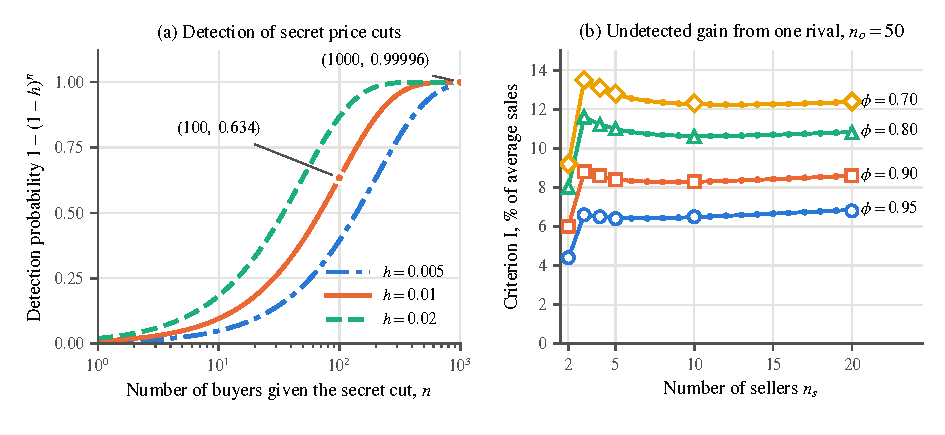
\includegraphics[width=\textwidth]{figures/ch02/stigler_detection.pdf}
\caption{Detection of secret price cutting. Panel (a) plots the probability that rivals hear of at least one secret cut
given to $n$ buyers, $1 - (1 - h)^n$, where $h$ is the probability that one cut is reported. The marked points are
Stigler's examples for $h = 0.01$. Panel (b) plots Stigler's Criterion I, \eqref{eq:02-stigler-crit1}, for $n_o = 50$
old buyers and four repeat probabilities $\phi$. Small dots are the formula at each integer $n_s$, and open markers
are the printed entries of \citet{Stigler1964}, Table 1. They coincide up to rounding.}
\label{fig:02-stigler-detect}
\end{figure}

\casehead{Criterion II: retaining one's own old customers}
A price cutter can also use secret cuts to keep more of its own old customers than usual. Without price cutting,
seller $i$ loses on average $(1 - \phi)\frac{n_o}{n_s}$ old customers, with variance $\sigma_1^2$. A single rival
has little basis for judging whether it receives a fair share of these. Stigler therefore assumes that the rivals
pool their information and suspect price cutting if seller $i$ loses fewer than
$(1 - \phi)\frac{n_o}{n_s} - 2\sigma_1$ customers, a 5 percent probability level. The cutter can then retain at most
$2\sigma_1$ extra old customers. As a share of its average sales, this is \emph{Criterion II},
\begin{equation}\label{eq:02-stigler-crit2}
G_{\mathrm{II}}(\phi, n_o, n_s) = \frac{2\sigma_1}{\frac{n_o}{n_s}} = 2\sqrt{\phi(1 - \phi)\,\frac{n_s}{n_o}} .
\end{equation}
It depends on the market only through the number of old customers per seller. Panel A of
\cref{tab:02-stigler-t234} reproduces part of Stigler's Table 2.

Comparing the two criteria shows that a price cutter is easier to detect through its gains from any one rival than
through an unusual rate of repeat sales. With $\phi = 0.95$ and 10 old customers per seller, Criterion II allows
13.8 percent. Table 1 gives the corresponding entries for one rival. They are 6.9 (2 sellers and 20 buyers), 8.9
(3 and 30), 7.4 (4 and 40), 6.4 (5 and 50) and 4.2 (10 and 100). Stigler adds two qualifications \citep[footnote 9]{Stigler1964}.
Multiplying the Table 1 entries by $n_s - 1$ gives the gain from all rivals together, which exceeds 13.8 percent
beyond two sellers. And Table 1 uses a looser probability level, so strict comparability would lower the Table 2
entries by one fifth. Stigler concludes that Criterion II will seldom be useful.

\casehead{Criterion III: new buyers}
New buyers form a flow rather than a stock, and Stigler takes the annual flow relative to old buyers as the unit.
Without price cutting, seller $i$ expects to sell to $m_3 = \frac{\lambda n_o}{n_s}$ new buyers, with binomial
variance $\sigma_3^2 = \left(1 - \frac{1}{n_s}\right)\frac{\lambda n_o}{n_s}$. Rivals cannot police this margin without
pooling information. With pooling, the seller is deemed a price cutter if it wins more than $m_3 + 2\sigma_3$ new
buyers, again a 5 percent level. Its total sales are $\frac{n_o(1 + \lambda)}{n_s}$ on average, so the largest
undetected gain as a share of sales is \emph{Criterion III},
\begin{equation}\label{eq:02-stigler-crit3}
G_{\mathrm{III}}(\lambda, n_o, n_s) = \frac{2\sigma_3}{\frac{n_o(1 + \lambda)}{n_s}}
= \frac{2}{1 + \lambda}\sqrt{\frac{(n_s - 1)\,\lambda}{n_o}} ,
\end{equation}
where the second equality uses $\sigma_3\frac{n_s}{n_o} = \sqrt{\frac{(n_s - 1)\lambda}{n_o}}$.

Panel B of \cref{tab:02-stigler-t234} reproduces part of Stigler's Table 3. The incentive to cut prices to new
buyers rises rapidly with the number of sellers, in proportion to $\sqrt{n_s - 1}$ for a given total of buyers. It
rises slowly when buyers per seller are held fixed. With $\lambda = \frac{1}{10}$ and 10 buyers per seller, it is
12.9 percent with 2 sellers and 17.7 percent with 20. It falls with the absolute number of buyers. Its dependence
on the rate of entry runs through the factor $\frac{\sqrt{\lambda}}{1 + \lambda}$, whose derivative has the sign of
$1 - \lambda$. The criterion therefore rises with $\lambda$ for $0 < \lambda < 1$, peaks at $\lambda = 1$ and falls
beyond it. With $n_o = 100$ and $n_s = 10$, it is 30 percent at $\lambda = 1$ and 24 percent at $\lambda = 4$. Rates
above one mean more new buyers per year than old buyers, and Stigler's Table 3 stays within $\lambda \le
\frac{1}{4}$. In that range, Stigler finds that when new buyers arrive at 10 percent per year or more, secret cuts
aimed at them yield larger undetected gains than poaching from any one rival. With $\phi = 0.90$, 100 old
buyers and 10 sellers, Criterion I allows 5.4 percent from each rival, while Criterion III with $\lambda =
\frac{1}{10}$ allows 17.2 percent in total. Markets in which new buyers arrive at such rates are therefore hard to
cartelize.

\begin{table}[htbp]
\centering
\caption{Stigler's Criteria II, III and IV (percent of average sales)}
\label{tab:02-stigler-t234}
\small
{\textit{Panel A. Criterion II: old customers a price cutter can retain (Table 2)}}\par\smallskip
\begin{tabular}{@{}lcccc@{}}
\toprule
& \multicolumn{4}{c}{Old customers per seller $\frac{n_o}{n_s}$} \\
\cmidrule(l){2-5}
Repeat probability $\phi$ & 10 & 20 & 50 & 100 \\
\midrule
0.95 & 13.8 & 9.7  & 6.2  & 4.4  \\
0.90 & 19.0 & 13.4 & 8.5  & 6.0  \\
0.80 & 25.3 & 17.9 & 11.3 & 8.0  \\
0.70 & 29.0 & 20.5 & 13.0 & 9.2  \\
0.50 & 31.6 & 22.4 & 14.1 & 10.0 \\
\bottomrule
\end{tabular}

\medskip
{\textit{Panel B. Criterion III: additional new customers obtainable (Table 3)}}\par\smallskip
\begin{tabular}{@{}cc*{6}{r}@{}}
\toprule
& & \multicolumn{6}{c}{Number of sellers $n_s$} \\
\cmidrule(l){3-8}
New-buyer rate $\lambda$ & Old buyers $n_o$ & 2 & 3 & 4 & 5 & 10 & 20 \\
\midrule
$\frac{1}{100}$ & 20  & 4.4 & 6.3 & 7.7 & 8.9 & 13.3 & 19.3 \\
                & 100 & 2.0 & 2.8 & 3.4 & 4.0 & 5.9  & 8.6  \\
                & 400 & 1.0 & 1.4 & 1.7 & 2.0 & 3.0  & 4.3  \\
\addlinespace
$\frac{1}{10}$  & 20  & 12.9 & 18.2 & 22.3 & 25.7 & 38.6 & 56.0 \\
                & 100 & 5.8  & 8.1  & 10.0 & 11.5 & 17.2 & 25.1 \\
                & 400 & 2.9  & 4.1  & 5.0  & 5.8  & 8.6  & 12.5 \\
\addlinespace
$\frac{1}{4}$   & 20  & 17.9 & 25.3 & 31.0 & 35.8 & 53.7 & 78.0 \\
                & 100 & 8.0  & 11.3 & 13.9 & 16.0 & 24.0 & 34.9 \\
                & 400 & 4.0  & 5.7  & 6.9  & 8.0  & 12.0 & 17.4 \\
\bottomrule
\end{tabular}

\medskip
{\textit{Panel C. Criterion IV: gain of a small firm against a large one, $\phi = 0.9$ (Table 4)}}\par\smallskip
\begin{tabular}{@{}cccccc@{}}
\toprule
& & \multicolumn{4}{c}{Size of large firm $K$} \\
\cmidrule(l){3-6}
Firms $n_s - K + 1$ & Buyers per small seller & 1 & 2 & 5 & 9 \\
\midrule
2  & 10 & 9.5 & 13.4 & 21.2 & 28.5 \\
2  & 50 & 4.2 & 6.0  & 9.5  & 12.7 \\
4  & 10 & 9.7 & 13.1 & 19.7 & 25.7 \\
10 & 10 & 5.4 & 7.2  & 10.7 & 14.0 \\
10 & 50 & 2.2 & 2.9  & 4.5  & 5.9  \\
\bottomrule
\end{tabular}

\medskip
\begin{minipage}{0.94\linewidth}
\footnotesize
Notes: Selected cells of \citet{Stigler1964}, Tables 2 to 4. Panel A uses \eqref{eq:02-stigler-crit2}, Panel B
uses \eqref{eq:02-stigler-crit3} and Panel C uses \eqref{eq:02-stigler-crit4}. We recomputed every printed cell of
the three tables. All agree to within 0.06 except one cell of Table 4 ($\phi = 0.9$, four firms, 50 buyers per
small seller, $K = 1$). It is printed as 4.0, while the formula gives 3.93 and the matching Table 1 cell is 3.9. In
Panel C, $n_s$ counts sellers in units of the small firm, so a firm of size $K$ counts as $K$ sellers.
\end{minipage}
\end{table}

\casehead{Pooling of information and unequal firm sizes}
With more than two sellers, firms can pool information and detect smaller deviations. The average number of old
customers that one cutter can take from $T$ rivals that pool information is at most
$\frac{T(1 - \phi)\,n_o}{n_s(n_s - T)}\bigl(1 + \frac{\tau}{\sqrt{T}}\bigr)$, with a correspondingly scaled variance.
For $T = 1$ this is $m_2$.
Both are smaller, relative to the customers lost by each pooling firm, than the corresponding expressions for one
seller. Pooling has limits. It becomes expensive as the pool grows, and it produces less reliable information,
because a member of the pool may itself be cutting prices.

Pooling by $K$ firms is equivalent to a single firm $K$ times as large as the others. Stigler's \emph{Criterion IV}
gives the gain of a small firm against such a large rival. It is measured as a percentage of the small firm's
average number of old customers, with $n_s$ counted in small-firm units:
\begin{equation}\label{eq:02-stigler-crit4}
G_{\mathrm{IV}} = \frac{1}{n_s - K}\left[\tau(1 - \phi)\sqrt{K}
+ \sqrt{\frac{n_sK(1 - \phi)(n_s - K - 1)\bigl(1 + \frac{\tau}{\sqrt{K}}\bigr)}{n_o}}\,\right].
\end{equation} For $K = 1$ it reduces to Criterion I. Compare Tables 1 and 4 for 100
customers, 10 firms and $\phi = 0.9$. A firm can take 5.4 percent of its sales from one rival, or about 50 percent
from all nine. If the nine rivals combine, Table 4 caps its gain at 28.5 percent.
In a second example with 20 firms and 200 customers, the gain from nine rivals falls from about 30 percent to 14.0
percent when they merge. Pooling information thus substantially reduces the scope for secret price cutting.
Stigler notes that Table 4 exaggerates the effect of size inequality. Only buyers above some size relative to the
seller are worth secret cuts, and a small firm can profitably cut prices to buyers too small to interest a large
seller.

\casehead{Repetition over time}
What may be chance in a single round cannot equally be chance if repeated. Over $T$ rounds, the mean loss to a
rival grows in proportion to $T$, while its standard deviation grows in proportion to $\sqrt{T}$. The threshold loss
over $T$ rounds is therefore $\frac{T(1 - \phi)}{n_s - 1}\cdot\frac{n_o}{n_s}\bigl(1 + \frac{\tau}{\sqrt{T}}\bigr)$.
The tolerated excess, relative to the mean, falls only as $\frac{1}{\sqrt{T}}$. Stigler concludes that this source of
information has minor efficacy unless buyers purchase, or sign contracts, frequently.

\subsubsection{Concentration and the Herfindahl index}

The model implies a measure of concentration suited to collusion. Suppose each new buyer picks firm $i$ with
probability equal to its output share $s_i$. Firm $i$'s number of new customers is then binomial with variance
$n_ns_i(1 - s_i)$. Summing over firms gives the total sampling noise against which price cutting must be detected,
\begin{equation}\label{eq:02-stigler-hhi}
\sum_{i} n_n s_i(1 - s_i) = n_n\Bigl(\sum_i s_i - \sum_i s_i^2\Bigr) = n_n(1 - \HHI) .
\end{equation}
The noise falls as the Herfindahl index rises. A similar argument applies to old customers
\citep[footnote 12]{Stigler1964}. Firm $j$ gains on average $(1 - \phi)n_o\frac{s_is_j}{1 - s_i}$ of the old customers
lost by firm $i$, with variance $(1 - \phi)n_o\frac{s_is_j}{1 - s_i}\bigl(1 - \frac{s_j}{1 - s_i}\bigr)$. Summing over
$i \ne j$ gives approximately $(1 - \phi)n_os_j(1 + \HHI - 2s_j)$. Summing over $j$ gives
$(1 - \phi)n_o(1 + \HHI - 2\HHI) = (1 - \phi)n_o(1 - \HHI)$. Stigler warns that the agreement of the two measures is
superficial, because the first assumes pooling of information and the second does not.

This gives a second foundation for the Herfindahl index, alongside the Cournot identity
$\bar L = \frac{\HHI}{\varepsilon}$ of \cref{prop:02-cowling-waterson}. The two arguments differ in kind. In Cournot,
a higher $\HHI$ raises margins under fixed noncooperative conduct. In Stigler's model, a higher $\HHI$ makes
collusion easier to police, so conduct itself changes. Both make the Herfindahl index more informative than a
four-firm ratio.

The analysis extends to nonprice competition with two modifications. There must be a definite joint
profit-maximizing policy to agree on, which is clearer for some variables than others. And nonprice moves differ in
detectability. Advertising, product quality and servicing leave visible traces, while reciprocal purchasing and
patent licensing do not. Collusion should suppress competition in the visible dimensions and leave it alive in the
hidden ones. The common belief that nonprice competition is more prevalent than price competition is therefore only
partly consistent with the theory.

The model's predictions can be collected. Collusion is easier to sustain when there are fewer sellers and when
buyers are numerous and small relative to sellers. A secret cut offered to many small buyers is likely to be
detected. Collusion is also easier when buyers are loyal ($\phi$ high) and new buyers arrive slowly ($\lambda$ low,
within $\lambda < 1$). It is easier still when sellers are unequal in size or pool information, when buyers report prices,
and when transactions are homogeneous enough for a simple price structure.

\subsubsection{Evidence}

Stigler's Section IV offers what he calls fragments of evidence. Two studies of the effect of the number of sellers
on price come first. He notes that, as far as he knows, no systematic analysis of this effect had been made
before.

\casehead{Newspapers and radio}
The first study concerns newspaper advertising rates in 53 cities in 1939. The rate per line per million
circulation, called the milline rate $R$, falls with circulation $z$. Stigler therefore first regresses
\begin{equation*}
\log R = 5.194 - \underset{(0.620)}{1.688}\,\log z + \underset{(0.063)}{0.139}\,(\log z)^2
\end{equation*}
He then tabulates the residuals by the number of evening papers in the city (Panel A of
\cref{tab:02-stigler-t56}). The mean residual is 0.0211 in one-paper cities and $-0.0213$ in two-paper cities.
Stigler reads this as rates about 5 percent above average in one-paper towns and 5 percent below in two-paper
towns. That reading matches base-10 logarithms, since $10^{0.0211} = 1.050$, while $e^{0.0211} = 1.021$.
Stigler adds that one-paper cities with an independent morning paper fall nearly midway between the two groups,
although their tabulated mean residual ($-0.0174$) lies close to the two-paper mean. Few cities had
more than two evening papers, so larger numbers of firms could not be studied. The subgroup means are internally
consistent: $\frac{10(-0.0174) + 13(0.0507)}{23} = 0.0211$.

The second study regresses the logarithm of AM radio spot rates on station characteristics for 345 stations in
Ohio, Indiana, Michigan and Illinois in 1961 (Panel B of \cref{tab:02-stigler-t56}). The elasticity of the rate with
respect to the number of stations in the county is $-0.074$, with a standard error of 0.046. The number of stations
ranges from 1 to 13 and is highly correlated with county population ($r^2 = 0.796$ in logarithms), which the
regression controls for. Both studies suggest that prices respond little to the number of rivals. Stigler finds this
consistent with his model, in which the number of buyers, the share of new buyers and the relative sizes of firms
matter as much as the number of sellers.

\begin{table}[htbp]
\centering
\caption{Number of sellers and prices in Stigler (1964)}
\label{tab:02-stigler-t56}
\small
{\textit{Panel A. Residuals from the regression of newspaper advertising rates on circulation, 1939 (Table 5)}}\par\smallskip
\begin{tabular}{@{}lccc@{}}
\toprule
Evening papers in city & Cities & Mean residual & Standard deviation of mean \\
\midrule
One                          & 23 & $0.0211$  & 0.0210 \\
\quad With morning paper     & 10 & $-0.0174$ & 0.0324 \\
\quad Without morning paper  & 13 & $0.0507$  & 0.0233 \\
Two                          & 30 & $-0.0213$ & 0.0135 \\
\bottomrule
\end{tabular}

\medskip
{\textit{Panel B. Regression of log AM spot commercial rates, 1961, $n = 345$ (Table 6)}}\par\smallskip
\begin{tabular}{@{}lcc@{}}
\toprule
Regressor & Coefficient & Standard error \\
\midrule
Log population of county, 1960              & $0.238$  & 0.026 \\
Log kilowatt power of station               & $0.206$  & 0.015 \\
Broadcast period: sunrise to sunset         & $-0.114$ & 0.025 \\
Broadcast period: longer, under 18 hours    & $-0.086$ & 0.027 \\
Broadcast period: 18 to 21 hours            & $-0.053$ & 0.028 \\
Log number of stations in county            & $-0.074$ & 0.046 \\
\midrule
$R^2$ & \multicolumn{2}{c}{0.743} \\
\bottomrule
\end{tabular}

\medskip
\begin{minipage}{0.94\linewidth}
\footnotesize
Notes: From \citet{Stigler1964}, Tables 5 and 6. Panel A: residuals, in logarithms, from
$\log R = 5.194 - 1.688\log z + 0.139(\log z)^2$, where $R$ is the milline rate and $z$ is circulation. The standard
errors of the slope coefficients are 0.620 and 0.063. Stigler's data come from the American Association of
Advertising Agencies. Panel B: the dependent variable is the logarithm of the average rate for 26 spots on May 1, 1961. The
broadcast-period variables are dummies. Table 6 does not state the omitted category. Stigler's data come from
the Standard Rate and Data Service.
\end{minipage}
\end{table}

\casehead{Profitability and concentration}
The direct test of the theory relates profitability to concentration across industries. Stigler restricts the
sample to 17 industries in which the sampled firms account for at least 35 percent of industry sales and earn at
least half of their revenue in the industry. Large steel and chemical firms, for example, operate in many markets
and are excluded. \Cref{tab:02-stigler-t7} reproduces his Table 7. Concentration in 1954 is measured by the four-firm
share and by the Herfindahl index. Profitability over 1953--57 is measured by the rate of return on all assets, the
rate of return on net worth, and the ratio of market to book value of common stock.

\begin{table}[htbp]
\centering
\begin{threeparttable}
\caption{Profitability and concentration in 17 industries (Stigler 1964)}
\label{tab:02-stigler-t7}
\small
\begin{tabular}{@{}lccccc@{}}
\toprule
& \multicolumn{2}{c}{Concentration, 1954} & \multicolumn{2}{c}{Average return, 1953--57} & Market to book \\
\cmidrule(lr){2-3}\cmidrule(lr){4-5}
Industry (firms) & Top-4 share & $\HHI$ & All assets & Net worth & value, 1953--57 \\
\midrule
\multicolumn{6}{@{}l}{\textit{Panel A. Industry data (Table 7)}} \\
Sulfur mining (4)                  & 98 & 0.407 & 19.03 & 23.85 & 3.02 \\
Automobiles (3)                    & 98 & 0.369 & 11.71 & 20.26 & 2.30 \\
Flat glass (3)                     & 90 & 0.296 & 11.79 & 16.17 & 2.22 \\
Gypsum products (2)                & 90 & 0.280 & 12.16 & 20.26 & 1.83 \\
Primary aluminum (4)               & 98 & 0.277 & 6.87  & 13.46 & 2.48 \\
Metal cans (4)                     & 80 & 0.260 & 7.27  & 13.90 & 1.60 \\
Chewing gum (2)                    & 86 & 0.254 & 13.50 & 17.06 & 2.46 \\
Hard-surface floor coverings (3)   & 87 & 0.233 & 6.56  & 7.59  & 0.98 \\
Cigarettes (5)                     & 83 & 0.213 & 7.23  & 11.18 & 1.29 \\
Industrial gases (3)               & 84 & 0.202 & 8.25  & 11.53 & 1.33 \\
Corn wet milling (3)               & 75 & 0.201 & 9.17  & 11.55 & 1.48 \\
Typewriters (3)                    & 83 & 0.198 & 3.55  & 5.39  & 0.84 \\
Domestic laundry equipment (2)     & 68 & 0.174 & 9.97  & 17.76 & 1.66 \\
Rubber tires (9)                   & 79 & 0.171 & 7.86  & 14.02 & 1.70 \\
Rayon fiber (4)                    & 76 & 0.169 & 5.64  & 6.62  & 0.84 \\
Carbon black (2)                   & 73 & 0.152 & 8.29  & 9.97  & 1.40 \\
Distilled liquors (6)              & 64 & 0.118 & 6.94  & 7.55  & 0.77 \\
\midrule
\multicolumn{6}{@{}l}{\textit{Panel B. Rank correlations with profitability (Table 8)}} \\
Top-4 share      & & & 0.322 & 0.507 & 0.642 \\
Herfindahl index & & & 0.524 & 0.692 & 0.730 \\
\bottomrule
\end{tabular}
\begin{tablenotes}\footnotesize
\item Notes: From \citet{Stigler1964}, Tables 7 and 8. The number of sampled firms is in parentheses. Returns are in
percent. In Panel B, each entry is the rank correlation between the concentration measure in the row and the
profitability measure in the column. Stigler reports a rank correlation of 0.903 between the two concentration
measures (his footnote 14). Our Spearman correlations computed from Panel A are 0.320, 0.499 and 0.652 for the
top-4 share. For $\HHI$ they are 0.525, 0.692 and 0.737, and between the two measures 0.903. The small differences
presumably reflect the treatment of ties.
\end{tablenotes}
\end{threeparttable}
\end{table}

All six rank correlations are positive. The Herfindahl index correlates more strongly with each profitability
measure than the four-firm share does, as the variance argument of \eqref{eq:02-stigler-hhi} suggests. Stigler
reads the data as showing no relation between profitability and concentration when $\HHI$ is below 0.250 or the
four-firm share is below about 80 percent. Our computations from Table 7 agree. Among the ten industries with
$\HHI < 0.250$, the Spearman correlations of $\HHI$ with the three profitability measures are $-0.03$, 0.18 and
0.11. The seven industries above the threshold earn on average 11.8 percent on assets, against 7.3 percent below
it. Stigler is careful about what this shows. The data, like those on advertising rates, ``confirm our theory only
in the sense that they support theories which assert that competition increases with number of firms.''

\casehead{Price cutting in steel}
The last piece of evidence uses prices paid by buyers of steel products in the second quarter of 1939, measured
relative to quoted prices. \Cref{tab:02-stigler-t9} reproduces Stigler's Table 9. The entry of 8.3 for hot-rolled
sheets, for example, is an average reduction of 8.3 percent from quoted prices, with a standard deviation of 7.3
percent of quoted prices. The average discount is almost perfectly correlated with the dispersion of transaction
prices. Our correlation across the eight products is 0.91. Stigler interprets this as expected: the less perfect the
market knowledge, the more extensive the price cutting.

\begin{table}[htbp]
\centering
\begin{threeparttable}
\caption{Prices of steel products and industry structure (Stigler 1964)}
\label{tab:02-stigler-t9}
\small
\begin{tabular}{@{}lcccc@{}}
\toprule
& \multicolumn{2}{c}{Prices, 2nd quarter 1939 (percent)} & & \\
\cmidrule(lr){2-3}
Product class & Average discount & Standard deviation & Herfindahl index & Output 1939 \\
& from list price & & & relative to 1937 \\
\midrule
Hot-rolled sheets   & 8.3 & 7.3 & 0.0902 & 1.14 \\
Merchant bars       & 1.2 & 4.5 & 0.1517 & 0.84 \\
Hot-rolled strip    & 8.5 & 8.3 & 0.1069 & 0.56 \\
Plates              & 2.6 & 4.8 & 0.1740 & 0.85 \\
Structural shapes   & 3.2 & 4.3 & 0.3280 & 0.92 \\
Cold-rolled strip   & 8.8 & 9.8 & 0.0549 & 0.88 \\
Cold-rolled sheets  & 5.8 & 5.0 & 0.0963 & 1.14 \\
Cold-finished bars  & 0.9 & 3.4 & 0.0964 & 0.83 \\
\bottomrule
\end{tabular}
\begin{tablenotes}\footnotesize
\item Notes: From \citet{Stigler1964}, Table 9, in his row order. The Herfindahl index uses 1938 capacity.
Transaction prices come from a Bureau of Labor Statistics survey reported in \textit{Iron Age} (1946). Capacity
data come from the \textit{Directory of Iron and Steel Works of the United States and Canada}, and output data
from the American Iron and Steel Institute. In our computations across the eight rows, the correlation of the
discount with its standard deviation is 0.91. The correlation of the discount with $\HHI$ is $-0.46$ (Spearman
$-0.55$), and the least-squares line is $\text{discount} = 7.40 - 18.09\,\HHI$.
\end{tablenotes}
\end{threeparttable}
\end{table}

The data show larger discounts in the less concentrated product classes. Cold-rolled strip has the lowest index,
0.0549, and the largest discount, 8.8 percent. Structural shapes have the highest index, 0.3280, and a discount of
3.2 percent. This is the ordering the theory predicts, since secret cuts are harder to police when sellers are
numerous and small. Stigler's summary sentence states the relation with the opposite sign. His remarks on
individual products fit the data. He notes that structural shapes and hot-rolled strip sold somewhat below the
average relationship, while cold-finished bars sold above it. In our fitted line, the first two have discounts 1.7
and 3.0 points above the line and cold-finished bars 4.8 points below. He adds that the deviations are not
explained by demand, measured by 1939 output relative to 1937. Our residuals are indeed uncorrelated with that
measure. The survey also excluded some very large buyers in the automobile and container industries. Since very
large buyers obtained the largest concessions, Stigler infers that the table understates price cutting.

Stigler judged these fragments ``fairly favorable to the theory,'' while granting that they do not constitute strong
support. He expected more powerful tests from the electrical equipment conspiracy cases then in the courts. The
theory predicts that prices on public bids will be higher and less dispersed than in privately negotiated sales.
It also predicts that price cutting increases as the number of buyers diminishes \citep[footnote 16]{Stigler1964}. He saw the
large number of testable hypotheses as the main merit of the theory.

\subsubsection{Assessment}

Stigler's paper made collusion an information problem. It gave the first systematic account of why cartels hold in
some markets and fail in others, and it tied cartel stability to observable features of markets. These include the
number and size distribution of sellers, the size and loyalty of buyers and the rate of arrival of new buyers.
They also include the transparency of transaction prices and the complexity of the price structure. Several of these ideas now organize
antitrust thinking about coordinated effects, from the role of large buyers to the danger of price transparency
(\cref{ch:collusion-evidence}).

The model has clear limits. It contains no equilibrium. Punishment after detection is asserted, as the matching of
detected cuts, and never derived. The price cutter does not choose how much to cut by weighing gains against the
risk of detection. The detection rules use fixed probability thresholds, such as one standard deviation, without a
decision-theoretic basis. The collusive price level is not determined, and the criteria measure the incentive to cut
by undetected sales alone, ignoring the margin on those sales. The evidence is cross-sectional and inherits the
endogeneity of market structure discussed in \cref{ch:intro}.

\citet{GreenPorter1984} read Stigler differently from the cross-industry tradition he inspired (pp.~87--88). In their
reading, Stigler justified cross-industry regressions by relating concentration informally to a cartel's ability to
deter cheating, and by assuming that profitability reflects cartel success. They recast his cartel as the solution
to a design problem: an institution that achieves an efficient outcome subject to the constraint that members act
noncooperatively. That shift leads directly to the repeated-game models of the next subsection.

\subsection{Repeated interaction: a preview}\label{sec:02-repeated}

Repeated interaction gives Stigler's enforcement a formal foundation. A deviation today can be punished tomorrow,
so collusive prices can be an equilibrium even though each firm gains by deviating in the short run. As in
\cref{sec:02-multiproduct} and \cref{ch:collusion-theory}, $\delta \in (0, 1)$ denotes the discount factor. The
stage game is played in periods $t = 0, 1, 2, \dots$, and each firm maximizes $\sum_{t \ge 0}\delta^t\pi_{it}$. We
use \emph{grim-trigger strategies}: firms play the collusive action as long as no one has deviated, and revert
forever to the static Nash equilibrium after any deviation \citep{Friedman1971}. Static Nash play forever is itself
a subgame-perfect equilibrium, so the threat is credible. The one-shot deviation principle, the folk theorem and
optimal punishments are developed in \cref{ch:collusion-theory}.

The horizon must be infinite \citep[sec.~11.3.2]{Tirole1988}. A repeated game has almost perfect information
(\cref{sec:02-spe}), so it can be solved by backward induction when it ends at a known date. If the stage game has a
unique Nash equilibrium, the stage equilibrium is then played in every period, and collusion unravels from the end
(\cref{prop:12-finite}). The Bertrand game has several equilibrium profiles, but all of them give zero profit, so the
same argument applies. With an infinite horizon there is no last period from which to start. Repeating the stage
equilibrium forever remains a subgame-perfect equilibrium, because no current action changes future play. Other
equilibria now exist, and they are sustained by the threat of reverting to the stage equilibrium after a deviation.
\Cref{prop:02-bertrand-collusion,prop:02-cournot-collusion} state when this threat suffices. We give the intuition
here and prove both results in \cref{sec:12-perfect}.

\begin{proposition}[Collusion in the Bertrand supergame]\label{prop:02-bertrand-collusion}
Let $N$ identical firms with constant marginal cost $c$ play the homogeneous Bertrand game of \cref{sec:02-bertrand}
in every period, with observed prices. Grim-trigger strategies with collusive price $p^m$ and Bertrand reversion form
a subgame-perfect equilibrium if and only if
\begin{equation}\label{eq:02-bertrand-ic}
\delta \ge 1 - \frac{1}{N} .
\end{equation}
\end{proposition}

\Cref{prop:12-bertrand} gives the proof. On the collusive path, conforming yields $\frac{\pi^m}{N}$ in every period,
worth $\frac{\pi^m}{N(1 - \delta)}$. The best deviation undercuts $p^m$ slightly, earns almost $\pi^m$ once, and
earns zero after the reversion to Bertrand pricing. Collusion is sustainable when $\frac{\pi^m}{N(1 - \delta)} \ge
\pi^m$, which is \eqref{eq:02-bertrand-ic}.

The threshold rises with $N$. Each firm's collusive share $\frac{\pi^m}{N}$ shrinks while the one-period gain from
deviation stays at about $\pi^m$. This is the formal version of Stigler's observation that collusion is impossible
for many firms. \citet[sec.~6.3.2.1]{Tirole1988} uses it to give Bain's link between concentration and tacit
collusion a precise sense.

\begin{example}[Detection lags]\label{ex:02-detection-lag}
Stigler's insight is that deviations are detected with delay. Suppose rivals learn of a secret price cut only with
probability $\mu \in (0, 1]$ in each period, for instance because random switching of buyers masks the lost sales.
Until detection, the cutter serves the market at a price just below $p^m$. Its deviation payoff becomes
\begin{equation*}
\pi^m\sum_{t \ge 0}\bigl[\delta(1 - \mu)\bigr]^t = \frac{\pi^m}{1 - \delta(1 - \mu)} .
\end{equation*}
Conforming is optimal if and only if
\begin{equation*}
\frac{\pi^m}{N(1 - \delta)} \ge \frac{\pi^m}{1 - \delta + \delta\mu}
\iff \delta\mu \ge (N - 1)(1 - \delta)
\iff \delta \ge \frac{N - 1}{N - 1 + \mu} .
\end{equation*}
With $\mu = 1$ this is \eqref{eq:02-bertrand-ic}. As $\mu \to 0$ the threshold tends to 1, and collusion becomes
impossible. If a cut reaches 100 buyers who each report it with probability $h = 0.01$, then
$\mu = 1 - (0.99)^{100} = 0.634$ from \eqref{eq:02-stigler-detect}. The threshold rises from 0.50 to 0.61 for
two firms and from 0.80 to 0.86 for five.
\end{example}

\begin{proposition}[Collusion in the linear Cournot supergame]\label{prop:02-cournot-collusion}
Let $N$ identical firms with constant marginal cost $c$ play the Cournot game with $P(Q) = a - bQ$ in every period.
Grim-trigger strategies with collusive output $\frac{Q^m}{N}$ each and reversion to the Cournot equilibrium form a
subgame-perfect equilibrium if and only if
\begin{equation}\label{eq:02-cournot-delta}
\delta \ge \delta^*(N) = \frac{(N + 1)^2}{N^2 + 6N + 1} .
\end{equation}
\end{proposition}

\Cref{prop:12-cournot} gives the proof. Let $\pi_c$, $\pi_d$ and $\pi_n$ be the per-period collusive, best
one-shot deviation and Cournot profits. A firm conforms if collusion forever is worth at least one period of
deviation profit followed by Cournot profit forever:
\begin{equation*}
\frac{\pi_c}{1 - \delta} \ge \pi_d + \frac{\delta\,\pi_n}{1 - \delta}
\iff \delta \ge \frac{\pi_d - \pi_c}{\pi_d - \pi_n} .
\end{equation*}
With linear demand the three profits are proportional to $\frac{(a - c)^2}{b}$, so the ratio depends only on $N$. It
simplifies to \eqref{eq:02-cournot-delta}.

The threshold is $\delta^*(2) = \frac{9}{17} = 0.529$, and it rises to 0.571, 0.643 and 0.752 for $N = 3, 5$ and
10. Its derivative is $\frac{4(N - 1)(N + 1)}{(N^2 + 6N + 1)^2} > 0$, and $\delta^*(N) \to 1$ as $N \to \infty$. The
comparison with Bertrand is instructive. For $N = 2$ the Cournot threshold is higher than the Bertrand value of
0.5. For $N \ge 3$ it is lower: 0.571 against 0.667 at $N = 3$, and 0.752 against 0.900 at $N = 10$. Two forces
work in opposite directions. Cournot reversion is a milder punishment than Bertrand reversion. But a Cournot
deviator cannot capture the whole market, because rivals' outputs stay fixed. With three or more firms the second
force dominates.

\casehead{Conduct as a reduced form of dynamic play}
In these models the static conduct parameter of \cref{sec:02-conduct} summarizes the outcome of dynamic play. It is
close to 1 in collusive phases and close to its Cournot or Bertrand value in punishment phases. \citet{Bresnahan1989}
draws the empirical implication directly from Stigler (pp.~1023--1025). If self-interest alone holds a collusive
arrangement together, uncertainty about rivals' behavior will sometimes trigger price wars even without actual
cheating. Data on a collusive industry should then show periods of cooperation and periods of competition.
``Empirically, of course, this will show up as time-varying $\theta$.'' Two models formalize the idea with
different predictions about when the price wars occur.

\casehead{Green and Porter: price wars after bad news}
\citet{GreenPorter1984} study cartel self-enforcement under demand uncertainty. In their model firms choose outputs,
and the market price depends on total output and an unobserved demand shock. Firms observe the price, but neither
rivals' outputs nor the shock. A low price may therefore signal either cheating or bad demand. The cartel uses a
trigger price. Firms produce collusive outputs while the price stays above the trigger and revert to Cournot output
for a fixed number of periods after it falls below. In equilibrium no firm cheats, yet low demand realizations set
off price wars. The wars are necessary, because without them cheating could not be deterred. Green and Porter
emphasize that earlier formulations make incentives so perfect that the deterrent mechanism is never observed. With
imperfect information, recurrent price wars are part of successful collusion. They need not indicate a sequence of
failed attempts to form a cartel (pp.~87--88).

A simple price-setting version conveys the logic. Two firms face demand $Q(p)$ with probability $1 - \zeta$ and
zero demand with probability $\zeta$, independently each period. A firm with zero sales cannot tell low demand from
a rival's secret cut. The strategy is to price at $p^m$ until a period of zero sales and then price at $c$
forever. The value of collusion is $V = \frac{(1 - \zeta)\frac{\pi^m}{2}}{1 - \delta(1 - \zeta)}$. A deviator earns
$(1 - \zeta)\pi^m$ once and nothing afterwards. Conforming is optimal if and only if
\begin{equation*}
\frac{(1 - \zeta)\frac{\pi^m}{2}}{1 - \delta(1 - \zeta)} \ge (1 - \zeta)\,\pi^m
\iff \delta(1 - \zeta) \ge \frac{1}{2} .
\end{equation*}
More noise ($\zeta$ higher) makes collusion harder, and price wars start after unexpectedly low demand.
\Cref{ch:collusion-theory} treats finite punishments and the optimal trigger, including the refinements of
\citet{AbreuPearceStacchetti1986}.

\casehead{Rotemberg and Saloner: price wars during booms}
\citet{RotembergSaloner1986} study implicitly colluding oligopolists facing fluctuating demand that they observe.
Their key finding is that the temptation to deviate from the collusive outcome is often greater when demand is high.
To moderate the temptation, the oligopoly lowers its prices in booms. Suppose demand states are independent over
time, and let $\pi_s(p)$ be industry profit at price $p$ in state $s$. With collusive prices $p_s$ and Bertrand
reversion, the incentive constraint in state $s$ is
\begin{equation*}
\left(1 - \frac{1}{N}\right)\pi_s(p_s) \le \frac{\delta}{1 - \delta}\cdot\frac{1}{N}\,\E\bigl[\pi_{s'}(p_{s'})\bigr] .
\end{equation*}
The left side is the gain from deviating in the current state, and it rises with current demand. The right side is
the expected future loss, which does not depend on the current state. In high-demand states the constraint binds
first, and the cartel must cap profits below the monopoly level by cutting price. The abstract of the 1984 working-paper
version cites supporting evidence from the railroads in the 1880s and the automobile industry in the 1950s. It
also cites the cyclical behavior of cement prices and price-cost margins.

\casehead{Implications for measurement}
Both models imply that conduct varies over time, but they disagree about the pattern. In Green and Porter, conduct
switches to the competitive value after unanticipated low demand and returns after a fixed lag. In Rotemberg and
Saloner, conduct varies within the collusive regime with the level of demand. \citet{Porter1983} estimated a supply
relation with two regimes for a nineteenth-century railroad cartel (\cref{ch:collusion-evidence}). Bresnahan notes
that the existence of regimes is easier to establish than their causes. Asking whether there are price wars uses all
periods of data, while asking what starts and stops them has as many observations as there are wars. Time variation
in conduct also complicates the interpretation of a constant estimated $\theta$, which is the critique of
\citet{Corts1999} developed in \cref{ch:conduct}.

\section{From homogeneous to differentiated products}\label{sec:02-bridge}

The theory so far assumed a homogeneous good. Few markets fit that description. Products differ in physical
characteristics, location, brand and service, even in markets that look homogeneous, such as pharmaceuticals with
chemically identical generics or retail gasoline. Electricity and refined sugar, the settings of two case studies in
\cref{ch:conduct}, come close to homogeneity. Most empirical questions in industrial organization need a model of
demand for differentiated products. Measuring market power, evaluating mergers, assessing taxes and tariffs,
analyzing product introductions and valuing new goods all depend on substitution patterns. With differentiated
products there is also no natural boundary for the market, so an estimated demand system can stand in for
market definition. This section shows how the pricing logic of this chapter carries over and points to where it is
developed.

A single-product firm $j$ that sets its price, taking rivals' prices as given, is a monopolist on its residual
demand $q_j(p)$, as in \cref{sec:02-residual}. The first-order condition
$q_j + (p_j - mc_j)\frac{\partial q_j}{\partial p_j} = 0$ gives the dollar markup and Lerner rules
\eqref{eq:02-dollar-markup} and \eqref{eq:02-lerner}, with the own-price derivative of residual demand in place
of the market derivative:
\begin{equation}\label{eq:02-single-product-markup}
p_j - mc_j = -\frac{q_j}{\frac{\partial q_j}{\partial p_j}} ,
\qquad
\frac{p_j - mc_j}{p_j} = \frac{1}{|\varepsilon_{jj}|} .
\end{equation}
For example, with logit demand and price coefficient $\alpha$, $\frac{\partial s_j}{\partial p_j} = -\alpha s_j(1 - s_j)$,
so the markup is $\frac{1}{\alpha(1 - s_j)}$. Pass-through follows the formulas of \cref{sec:02-passthrough}, and for
the logit it equals $1 - s_j$ when rivals' prices are held fixed (\cref{ex:02-pt-examples}).

A firm that owns several products adds a new term. Let firm $f$ own the set $\mathcal{J}_f$ and maximize
$\sum_{k \in \mathcal{J}_f}(p_k - mc_k)\,q_k(p)$ over its own prices. The first-order condition for $p_j$,
$j \in \mathcal{J}_f$, is
\begin{equation*}
q_j + (p_j - mc_j)\frac{\partial q_j}{\partial p_j} + \sum_{k \in \mathcal{J}_f\setminus\{j\}}(p_k - mc_k)\frac{\partial q_k}{\partial p_j} = 0 .
\end{equation*}
Divide by $\frac{\partial q_j}{\partial p_j} < 0$, solve for $p_j$, and define the \emph{diversion ratio}
$D_{jk} = -\frac{\partial q_k}{\partial p_j}\bigl(\frac{\partial q_j}{\partial p_j}\bigr)^{-1}$, the fraction of the sales lost by
product $j$ that product $k$ recaptures when $p_j$ rises. Then
\begin{equation}\label{eq:02-diversion-foc}
p_j = mc_j - \frac{q_j}{\frac{\partial q_j}{\partial p_j}} + \sum_{k \in \mathcal{J}_f\setminus\{j\}}(p_k - mc_k)\,D_{jk} .
\end{equation}
Price equals marginal cost, plus the single-product markup, plus the margins the firm earns on sales recaptured by
its other products. The last term is an opportunity cost of selling product $j$, since each sale partly
cannibalizes the firm's other products. Joint ownership of substitutes therefore raises prices. A merger adds the
acquired products to $\mathcal{J}_f$ and the corresponding terms to \eqref{eq:02-diversion-foc}. This is the logic
of upward pricing pressure in \cref{ch:mergers}. The homogeneous-goods analogue is the gap between Cournot conduct,
in which each firm ignores its effect on rivals, and collusion, in which it internalizes all of it
(\cref{prop:02-cheat}).

When one firm owns every product, this first-order condition is the condition \eqref{eq:02-multi-foc-margin} of the
multiproduct monopolist in \cref{sec:02-multiproduct}. The diversion-ratio form is the same condition divided by
the own-price derivative. To see the link with the Lerner form, substitute $\frac{\partial q_k}{\partial p_j} =
\varepsilon_{kj}\frac{q_k}{p_j}$ and $\frac{\partial q_j}{\partial p_j} = -\lvert\varepsilon_{jj}\rvert\frac{q_j}{p_j}$
into the definition of the diversion ratio:
\[
  D_{jk} = \frac{\varepsilon_{kj}\,q_k}{\lvert\varepsilon_{jj}\rvert\,q_j} .
\]
The single-product markup is $-q_j\bigl(\frac{\partial q_j}{\partial p_j}\bigr)^{-1} =
\frac{p_j}{\lvert\varepsilon_{jj}\rvert}$.
Dividing \eqref{eq:02-diversion-foc} by $p_j$ and writing $R_j = p_jq_j$ then gives
\[
  \frac{p_j - mc_j}{p_j} = \frac{1}{\lvert\varepsilon_{jj}\rvert}
  + \sum_{k \in \mathcal{J}_f\setminus\{j\}}\frac{(p_k - mc_k)\,q_k\,\varepsilon_{kj}}{R_j\,\lvert\varepsilon_{jj}\rvert} ,
\]
which is \eqref{eq:02-multi-lerner} with the sum restricted to the firm's own products. Positive diversion
corresponds to substitutes in that formula, and it raises the Lerner index above the inverse own elasticity.

Stacking \eqref{eq:02-diversion-foc} over products gives the matrix form $p = mc - (\Omega \odot \Delta^\top)^{-1}q$,
with ownership matrix $\Omega$ ($\Omega_{jk} = 1$ if $j$ and $k$ have the same owner) and demand Jacobian $\Delta$,
whose $(j,k)$ element is $\frac{\partial q_j}{\partial p_k}$. \Cref{ch:diffprod} develops this system, the existence
and uniqueness of equilibrium, the recovery of marginal costs from estimated demand, and the demand models that
supply the derivatives. Theory in this area mostly studies prices and products given a demand system. Empirical work
does the reverse: it models demand richly and supply simply, usually as static Bertrand-Nash pricing. Richer demand
models add assumptions and computation, so they should be judged by what they add for the question at hand and the
data available.


\section{Bibliographic notes}\label{sec:02-notes}

\citet{Tirole1988} remains the standard textbook treatment of the theory in this chapter. The electronic edition we
used has no printed page numbers, so we cite it by chapter, section, equation and exercise. Its chapter~1 (secs.~1.1
to 1.5) covers single-product and multiproduct monopoly, the deadweight loss and the output subsidy
(\cref{sec:02-monopoly,sec:02-welfare}). It also treats cost distortions, rent seeking and the limits that recycling
and durability place on monopoly power. Chapter~5 covers Bertrand competition, rationing and capacity constraints in
secs.~5.1 to 5.3 (\cref{sec:02-bertrand}). Its secs.~5.4 and 5.5 treat Cournot competition and concentration
indices, and sec.~5.7 treats existence, convergence and the capacity-price game
(\cref{sec:02-measures,sec:02-cournot}). Section~6.3 treats
the supergames previewed in \cref{sec:02-repeated}. Chapter~11 is a user's manual for the game theory of
\cref{sec:02-games}, and \citet{FudenbergTirole1991} give a complete treatment. \citet{Shapiro1989} surveys static
and dynamic oligopoly theory, and \citet{Vives1999} develops existence, uniqueness and comparative statics with the
tools of aggregative and supermodular games.

The aggregative proof of \cref{prop:02-cournot-exist} goes back to \citet{SzidarovszkyYakowitz1977} and
\citet{Novshek1985}. The effects of entry on Cournot outcomes go back to \citet{Seade1980}, and the
margin-concentration identity to \citet{CowlingWaterson1976}. \citet{EncaouaJacquemin1980} give the axioms for
concentration indices. \citet{Demsetz1973} gives the efficiency explanation of the link between concentration and
profit. \citet{DansbyWillig1979} give the welfare interpretation of the Herfindahl index.
\citet{BulowGeanakoplosKlemperer1985} introduced the language of strategic substitutes and complements.
\citet{Edgeworth1925}, first published in 1897, showed that capacity limits undo the Bertrand outcome.
\citet{Beckmann1967} and \citet{LevitanShubik1972} solved the capacity-constrained price game.
\citet{KrepsScheinkman1983} and \citet{DavidsonDeneckere1986} are the key papers on capacity commitment and price
competition, and \citet{Gertner1985} studies the game in which capacities are not observed.
\citet{KlempererMeyer1989} develop supply function equilibria.

The conduct parameter and its interpretation are best read in \citet{Bresnahan1989}, which also gives the menu of
conduct for leaders, fringes and collusive regimes. \citet{Corts1999} shows why a constant estimated $\theta$ need
not measure average conduct, a point that \cref{ch:conduct} develops. The theory of pass-through starts with
\citet{BulowPfleiderer1983}, and \citet{WeylFabinger2013} unify pass-through and incidence under imperfect
competition. \citet{Sumner1981} and \citet{GenesoveMullin1998} use pass-through and the Bulow-Pfleiderer demand
family to measure conduct.

The welfare analysis of free entry follows \citet{MankiwWhinston1986}, who build on \citet{Spence1976} and
\citet{DixitStiglitz1977} for the case of product diversity. \citet{BerryWaldfogel1999} measure the inefficiency of
free entry in radio broadcasting, an empirical test of the excess-entry theorem. The 1996 working-paper version
(NBER Working Paper 5528), which we cite here, uses data on advertising prices, numbers of stations and listening in 135
US metropolitan markets. Relative to the social optimum, the welfare loss of free entry is 40 percent of industry
revenue, counting market participants other than listeners. Free entry would be optimal if the marginal value of
programming to listeners exceeded three times the value of marginal listeners to advertisers, who pay 4.5 cents per
hour. \Cref{ch:diffprod} returns to this paper.

The deadweight loss of monopoly was first estimated by \citet{Harberger1954}. \citet{Posner1975} added the costs of
rent-seeking, and \citet{Fisher1985} questioned the conditions under which rents are fully dissipated.
\citet[pp.~739 and 743]{CowlingMueller1978} found losses of up to 13 percent of gross corporate product in the
United States and 7.2 percent in the United Kingdom once rent-seeking costs are counted. \citet{JennyWeber1983} also
found large losses, and \citet{Scherer1980} doubts these high estimates \citep[sec.~1.1.1.2]{Tirole1988}.
\citet{Leibenstein1966} named X-inefficiency, and \citet{Coase1972} posed the problem of
the durable-good monopolist. \citet{Williamson1968} framed the trade-off between market power and cost savings that
merger policy still uses.

\citet{Stigler1964} founded the information-based theory of collusion. \citet{Friedman1971} gave the first
repeated-game model of collusion with trigger strategies, and \citet{GreenPorter1984} and
\citet{RotembergSaloner1986} showed how imperfect monitoring and demand fluctuations generate price wars.
\citet{AbreuPearceStacchetti1986} characterized optimal cartel equilibria under imperfect monitoring. \Cref{ch:collusion-theory} develops these models
and \cref{ch:collusion-evidence} confronts them with data.

\section{Exercises}\label{sec:02-exercises}

\begin{enumerate}[label=\arabic*., leftmargin=*, itemsep=6pt]

\item \textit{Cournot competition with constant-elasticity demand.} Inverse demand is
$P(Q) = \left(\frac{Q}{A}\right)^{-\frac{1}{\varepsilon}}$ with $A > 0$ and $\varepsilon > 0$, and $N$ firms have
the same constant marginal cost $c > 0$.
\begin{enumerate}[label=(\alph*)]
  \item Derive the symmetric Cournot equilibrium price and the Lerner index. Show that an interior equilibrium
  requires $N\varepsilon > 1$, and check the second-order condition at the equilibrium.
  \item Show that the firm-level inequality $P'(Q) + q_iP''(Q) < 0$ of \cref{rem:02-c2}, evaluated at the symmetric
  equilibrium, holds if and only if $N\varepsilon > 1 + \varepsilon$. Give an example with $N = 2$ in which an
  interior equilibrium exists although this inequality fails at the equilibrium. Are quantities strategic
  substitutes or complements there?
  \item Assume $N\varepsilon > 1 + \varepsilon$. Use \cref{prop:02-pt-cournot} to compute the pass-through of a
  common cost shock and of a shock to one firm's cost. Compare the two with the monopoly rate $\frac{\varepsilon}{\varepsilon - 1}$ and explain why a more
  competitive industry passes through less.
\end{enumerate}

\item \textit{Consistent conjectures.} Two firms face $P(Q) = a - bQ$ and have the cost function
$C(q) = cq + \frac{k}{2}q^2$ with $k \ge 0$. Each firm holds the constant conjecture
$r = \frac{\dd q_j}{\dd q_i}$, the conjectural variation of \cref{sec:02-aggregation} with one rival.
\begin{enumerate}[label=(\alph*)]
  \item Derive firm $i$'s first-order condition and its reaction function. Show that the reaction function has slope
  $-\frac{b}{(2 + r)b + k}$.
  \item A conjecture is \emph{consistent} if it equals the slope of the rival's reaction function. Show that with
  $k = 0$ the only consistent conjecture is $r = -1$, and that it yields price equal to marginal cost.
  \item Show that with $k > 0$ the consistent conjecture lies in $(-1, 0)$. Compute the implied industry conduct
  parameter.
  \item Explain why consistency does not answer the critique of conjectural variations in
  \cref{sec:02-interpret}.
\end{enumerate}

\item \textit{Constant pass-through.} Complete the proof of \cref{prop:02-pt-constant}.
\begin{enumerate}[label=(\alph*)]
  \item Suppose monopoly pass-through equals a constant $\rho > 0$ on an interval of costs. Show that
  $\frac{QP''(Q)}{P'(Q)} = \frac{1}{\rho} - 2$ on the corresponding interval of outputs.
  \item Solve this differential equation for $P'$, and then for $P$. Show that $P(Q) = a - bQ^{\gamma}$ with
  $\gamma = \frac{1}{\rho} - 1$ when $\rho \ne 1$, and $P(Q) = a - b\ln Q$ when $\rho = 1$.
  \item Identify the members of the family with linear, quadratic and constant-elasticity demand, and state the
  restrictions on $(a, b, \gamma)$ that make demand downward sloping and satisfy the second-order condition.
  \item Show that pass-through is also constant under any constant conduct $\theta$, and find its value.
\end{enumerate}

\item \textit{Specific and ad valorem taxes under monopoly.} A monopolist with constant marginal cost $c > 0$ faces
$Q(p) = Ap^{-\varepsilon}$ with $\varepsilon > 1$.
\begin{enumerate}[label=(\alph*)]
  \item Derive the price under a specific tax $t$ and under an ad valorem tax at rate $t_a$ (\cref{rem:02-pt-adval}).
  Compute $\frac{\dd p}{\dd t}$ and $\frac{\dd p}{\dd t_a}$ at zero taxes.
  \item Use \cref{prop:02-incidence} and the envelope theorem to compute the consumer burden, the producer burden and
  the tax revenue of each tax at the margin, starting from zero taxes.
  \item Normalize both taxes to raise one dollar of revenue at the margin. Which tax imposes the smaller burden on
  consumers, and which the smaller loss of total surplus? Explain the answer in terms of the effect of each tax on
  the firm's markup.
\end{enumerate}

\item \textit{Excess entry.} Use the linear Cournot market of \cref{ex:02-mw-linear} with $a - c = 8$ and $b = 1$.
\begin{enumerate}[label=(\alph*)]
  \item Find the set-up cost $F$ for which the second-best number of firms is $N^o = 4$.
  \item Compute the free-entry number of firms with $N$ treated as continuous and as an integer.
  \item Compute total surplus at $N^o$ and at the integer $N^e$, and express the loss as a percentage of the maximal
  surplus $\frac{(a - c)^2}{2b}$.
  \item Show that, with $N$ continuous, the loss as a share of the maximal surplus depends on the primitives only
  through $N^o$. Explain why the loss shrinks as $N^o$ grows although $N^e - N^o$ grows.
\end{enumerate}

\item \textit{Partial collusion in a Cournot duopoly.} Two firms with constant marginal cost $c$ face
$P(Q) = a - bQ$ in every period, discount the future by $\delta$ and use grim-trigger strategies with Cournot
reversion. They agree on a symmetric
output $q$ per firm, between the collusive output $\frac{a - c}{4b}$ and the Cournot output $\frac{a - c}{3b}$.
\begin{enumerate}[label=(\alph*)]
  \item Compute the per-period profit from conforming, the profit from the best one-period deviation, and the Cournot
  profit, as functions of $q$.
  \item Show that the incentive constraint holds if and only if
  $q \ge \frac{(a - c)(9 - 5\delta)}{b(27 - 3\delta)}$.
  \item Conclude that firms with $\delta < \frac{9}{17}$ can still sustain prices above the Cournot level. Plot the
  implied conduct parameter $\theta(\delta)$ against $\delta \in [0, 1)$ and relate the result to the time-varying
  conduct of \cref{sec:02-repeated}.
\end{enumerate}

\item \textit{Stigler's model of detection.}
\begin{enumerate}[label=(\alph*)]
  \item Use \eqref{eq:02-stigler-crit1} to compute Criterion I for $\phi = 0.9$, $n_o = 100$ and $n_s = 5$, and check
  your answer against \cref{tab:02-stigler-t1}.
  \item Show that, as $n_o \to \infty$ with $n_s$ and $\phi$ fixed,
  \[
    \sqrt{n_o}\,G_{\mathrm{I}} \to \frac{1}{n_s - 1}\left[\sqrt{\phi(1 - \phi)n_s} + \sqrt{n_s(n_s - 2)(1 - \phi)}\right].
  \]
  Interpret the result in terms of the number of buyers per seller.
  \item Derive \eqref{eq:02-stigler-hhi}. Construct two markets with the same four-firm concentration ratio and
  different Herfindahl indices, and say in which one Stigler's theory predicts more effective collusion.
  \item List two features of a modern repeated-game model of collusion that Stigler's model lacks, and explain how
  each changes the predictions in (b) and (c).
\end{enumerate}

\item \textit{Interpreting a pass-through estimate.} A regression of the retail price of a product on a specific
excise tax, across regions and years, gives $\hat\rho = 1.07$ with a small standard error.
\begin{enumerate}[label=(\alph*)]
  \item Use \cref{cor:02-pt-reveal} to state what this estimate rules out. List the maintained assumptions behind the
  conclusion.
  \item Describe the set of pairs $(\chi, \theta)$ consistent with the estimate when marginal cost is flat. Which
  value of $\theta$ does it imply if demand has constant elasticity $\varepsilon = 1.5$? If demand is linear?
  \item The price variable is an average over brands. Explain how the composition effect of
  \cref{rem:02-pt-composition} could produce $\hat\rho > 1$ in a competitive industry, and describe a test.
  \item Suppose instead that the tax applied to one of $N$ Cournot firms only. What would an estimate of 1.07 then
  imply about the curvature of demand, by \cref{prop:02-pt-cournot}?
\end{enumerate}

\end{enumerate}
